
%!TEX TS-program = lualatex
%!TEX encoding = UTF-8 Unicode


%\documentclass[11pt,b5paper]{book}
% \usepackage{fontspec}
% \defaultfontfeatures{Mapping=tex-text}
%\usepackage{amsmath}
%\usepackage{amssymb}
%\usepackage{euler}
%		\usepackage{geometry}
% setting page parameters
%		\geometry{textwidth=5in, textheight=7.5in,  marginparsep=7pt, marginparwidth=.6in}
%\usepackage{longtable}
\documentclass[10pt]{scrbook}
\usepackage{geometry}                % See geometry.pdf to learn the layout options. There are lots.
\geometry{paperheight=150mm,paperwidth=150mm, textwidth=75mm, textheight=100mm,                 top=20mm, bottom=20mm, marginparwidth=40mm, headsep=8mm, left=10mm, right=55mm, marginparsep=5mm, footskip=10mm}                   % ... or a4paper 

% to see the page layout
%\usepackage{showframe}


\usepackage[parfill]{parskip}    % Activate to begin paragraphs with an empty line rather than an indent


\usepackage{graphicx}
%\usepackage[]{gfsneohellenic}
\usepackage{amsmath}

\usepackage{amssymb}



%\usepackage[sfdefault]{josefin}
\usepackage[libertine]{newtxmath}
\usepackage[nomath]{libertinus}

\usepackage{marginnote}
\usepackage{sidenotes}
\renewcommand*{\marginfont}{\footnotesize}
\renewcommand\raggedrightmarginnote{}
\renewcommand\raggedleftmarginnote{}

\makeatletter
\ExplSyntaxOn
\RenewDocumentCommand \@sidenotes@placemarginal { m m }
{
  \IfNoValueOrEmptyTF{#1}
    % substitue \marginnote from marginnote pkg for \marginpar 
    % from latex2e format
    {\marginnote{#2}}
    {\marginnote{#2}[#1]}
}
\ExplSyntaxOff
\makeatother
%https://tex.stackexchange.com/questions/532245/how-to-modify-fonts-in-sidenotes

\usepackage{soul}
\usepackage[tracking=smallcaps,letterspace=100]{microtype}


\addtokomafont{chapter}{\color{darkgray}}
\addtokomafont{section}{\color{gray}}
\addtokomafont{subsection}{\color{LightSlateGray}}
\setkomafont{caption}{\small\sffamily}

\setlength{\textfloatsep}{0.9\baselineskip plus 0.2\baselineskip minus 0.5\baselineskip}

\RedeclareSectionCommand[beforeskip=.5\textheight plus 1.25\baselineskip]{chapter}

%\newcommand{\alignedmarginpar}[1]{%
%    \marginpar[\raggedleft #1]{\raggedright #1}%
%}
%https://tex.stackexchange.com/questions/411939/marginpar-text-alignment

%\newcommand{\ans}{\alignedmarginpar{\textcolor{SteelBlue}{{\strut\large \emph{Answer}}}}}% prints in red
%
%\newcommand{\ques}{\alignedmarginpar{\textcolor{Salmon}{{\strut\large \emph{Question}}}}}% prints in red

\newcommand{\ques}{\textcolor{Salmon}{\large \emph{Question\quad}}}% prints in red
\newcommand{\ans}{\textcolor{SteelBlue}{\large \emph{Answer\quad}}}


\newcommand{\drkgry}[1]{\textcolor{darkgray}{{#1}}}

% Redefine \partpagestyle to empty
\renewcommand*{\partpagestyle}{empty}

\usepackage[per-mode=symbol]{siunitx}
\sisetup{
  group-separator={,},
  group-minimum-digits=4,
}


\usepackage{booktabs}
%\usepackage{concmath}
%\usepackage{kpfonts}
\usepackage{enumitem}

\usepackage[usenames,dvipsnames,svgnames,table]{xcolor}

% \usepackage{colortbl}
\usepackage{multicol}
%\usepackage{mathtools}
\usepackage{nicefrac}

\usepackage{graphicx}


% for numbers/text with circles around them
% hyper referencing objects urls etc
\usepackage[colorlinks = true, urlcolor=DodgerBlue, linkcolor=darkgray, citecolor=DodgerBlue,linktoc=all]{hyperref}


\RedeclareSectionCommand[
  runin=false,
  afterindent=false,
  beforeskip=.5\baselineskip,
  afterskip=5pt]{section}
  
%\usepackage{basicarith}
%\usepackage{xlop}
% Adjust the space after floats
% Define a new command for easier spacing adjustment

\newcommand*\figr[1]{\hyperref[#1]{Figure~\ref{#1}}}

\usepackage{emptypage}

\usepackage{epigraph}

%\usepackage{tikz}

\usepackage{physics}
\usepackage{pdfpages}
\usepackage{relsize}


\usepackage{chngcntr}
\counterwithout{figure}{chapter}
\let\widering\relax
%
\usepackage{yhmath}
\DeclareFontFamily{OMX}{yhex}{}
\DeclareFontShape{OMX}{yhex}{m}{n}{<->yhcmex10}{}
\DeclareSymbolFont{yhlargesymbols}{OMX}{yhex}{m}{n}
\DeclareMathAccent{\wideparen}{\mathord}{yhlargesymbols}{"F3}
% https://tex.stackexchange.com/questions/96680/a-better-notation-to-denote-arcs-for-an-american-high-school-textbook


\AtBeginEnvironment{quote}{\smaller}%

\usepackage{dvgloss}



\usepackage{fullwidth}

\usepackage{tikz}
\usetikzlibrary{tikzmark,arrows}
\usepackage{calc} % for '\widthof' macro


%%%%%%  END OF PACKAGES 

\title{Geometry for Entertainment}
\author{Yakov Perelman}
\date{2024}


%%%% META DATA

\begin{document}
\renewcommand{\baselinestretch}{1}\normalsize


\includepdf{figures/perelman-geometry-fc.pdf}

\frontmatter

% !TEX root = perelman-geometry.tex
%!TEX TS-program = pdflatex
%!TEX encoding = UTF-8 Unicode


\maketitle
\cleardoublepage
\thispagestyle{empty}
%\pagenumbering{roman}
\begin{center}

{\LARGE Ya. I. Perelman}

{\Huge Geometry for Entertainment}




The Mir Titles Project

\end{center}
\cleardoublepage

\thispagestyle{empty}
\vfill

{\noindent
Seventh Edition, Revised

Edited and supplemented by B. A. Kordemsky

First Published by State Publishing House Of Technical And Theoretical Literature Moscow -- 1950 -- Leningrad.

Original scan in Russian by the Russian Lutherean on The Internet Archive \url{https://archive.org/details/20220910_perelman_geometry/}.

Translated from the Russian and typeset in \LaTeX{} by \emph{Damitr Mazanav}.

This fully electronic English translation released on the web by \emph{The Mir Titles Project}. \url{https://mirtitles.org} in 2024.

 


Licence Creative Commons by SA 4.0

\cleardoublepage

 \tableofcontents
 
 \cleardoublepage

\chapter{Editor's Preface}
\label{editor-preface}
%\addcontentsline{toc}{chapter}{\nameref{preface}}


\emph{Geometry for Entertainment} is written both for friends of mathematics and for those readers from whom many attractive aspects of mathematics have somehow been hidden.

More importantly, this book is intended for those readers who studied (or are currently studying) geometry only at the blackboard and therefore are not used to noticing familiar geometric relationships in the world of things and phenomena around us, have not learnt to use the acquired geometric knowledge in practise, in difficult cases of life, on a hike, in a bivouac or front-line situation.

To arouse the reader's interest in geometry or, in the words of the author, ``to inspire a desire and cultivate a taste for its study is the objective of this book.''

To this end, the author will take geometry ``out of the walls of the school room into the free air, into the forest, field, to the river, on the road, in order to indulge in relaxed geometric studies without a textbook and tables in the open air \ldots{}'', and draws the reader's attention to the pages of L. N. Tolstoy and A. P. Chekhov, Jules Verne and Mark Twain. He finds a theme for geometric problems in the works of N. V. Gogol and A. S. Pushkin, and finally offers the reader ``a motley selection of problems, curious in plot, unexpected in result.''

The seventh edition of \emph{Geometry for Entertainment} is published without the direct participation of the author. Ya. I. Perelman died in Leningrad in 1942.

The new edition of the book contains almost all the articles of the previous edition, newly illustrated, edited and supplemented with facts and information from our Soviet reality, as well as a considerable number (about 30) additional articles.

I was guided by the desire to increase the ``utility coefficient'' of Ya. Perelman's book, to make it even more effective and interesting, involving new readers in the ranks of friends of mathematics.

To what extent this was possible, I hope to learn from readers at the address: Moscow, 64, Chernyshevsky Str., 81, Sq. 53, B. A. Kordemsky.


\begin{flushright}
\emph{B. Kordemsky}
\end{flushright}


\chapter{Translator's Preface}
\label{translator-preface}
%\addcontentsline{toc}{chapter}{\nameref{preface}}

Yakov Perelman's books have been a constant source of inspiration for me throughout my life. It brings me great pleasure to present this as of now untranslated work of Perelman to English world. 

I have tried my level best to create a readable version of the translation. If there are any mistakes they are all mine. Any suggestions and criticisms to improve the translation are welcome. I hope that this English version finds enthusiastic readers.

\begin{flushright}
\emph{Damitr Mazanav}
\end{flushright}



\mainmatter

\part{Geometry In The Open Air}

% !TEX root = perelman-geometry.tex
%!TEX TS-program = pdflatex
%!TEX encoding = UTF-8 Unicode

% epigraph for part 1

\cleardoublepage
\vspace*{\fill}
\begin{center}
\epigraph{\begin{minipage}{0.4\pagewidth} \textsf{Nature speaks the language of mathematics: the letters of this language are circles, triangles and other mathematical shapes.}\end{minipage}}{Galileo}
\end{center}
\vspace*{\fill}

\thispagestyle{empty}

% begin chapter

\cleardoublepage

%\RedeclareSectionCommand[beforeskip=2.75cm]{chapter}
%\RedeclareSectionCommand[afterskip=1cm]{chapter}
%\RedeclareSectionCommand[beforeskip=0.1\baselineskip,afterskip=0.25\baselineskip]{section}
%
%\RedeclareSectionCommand[beforeskip=-1cm]{section}
%\vspace*{2cm} % Adjust the value as needed

\setchapterpreamble[o]{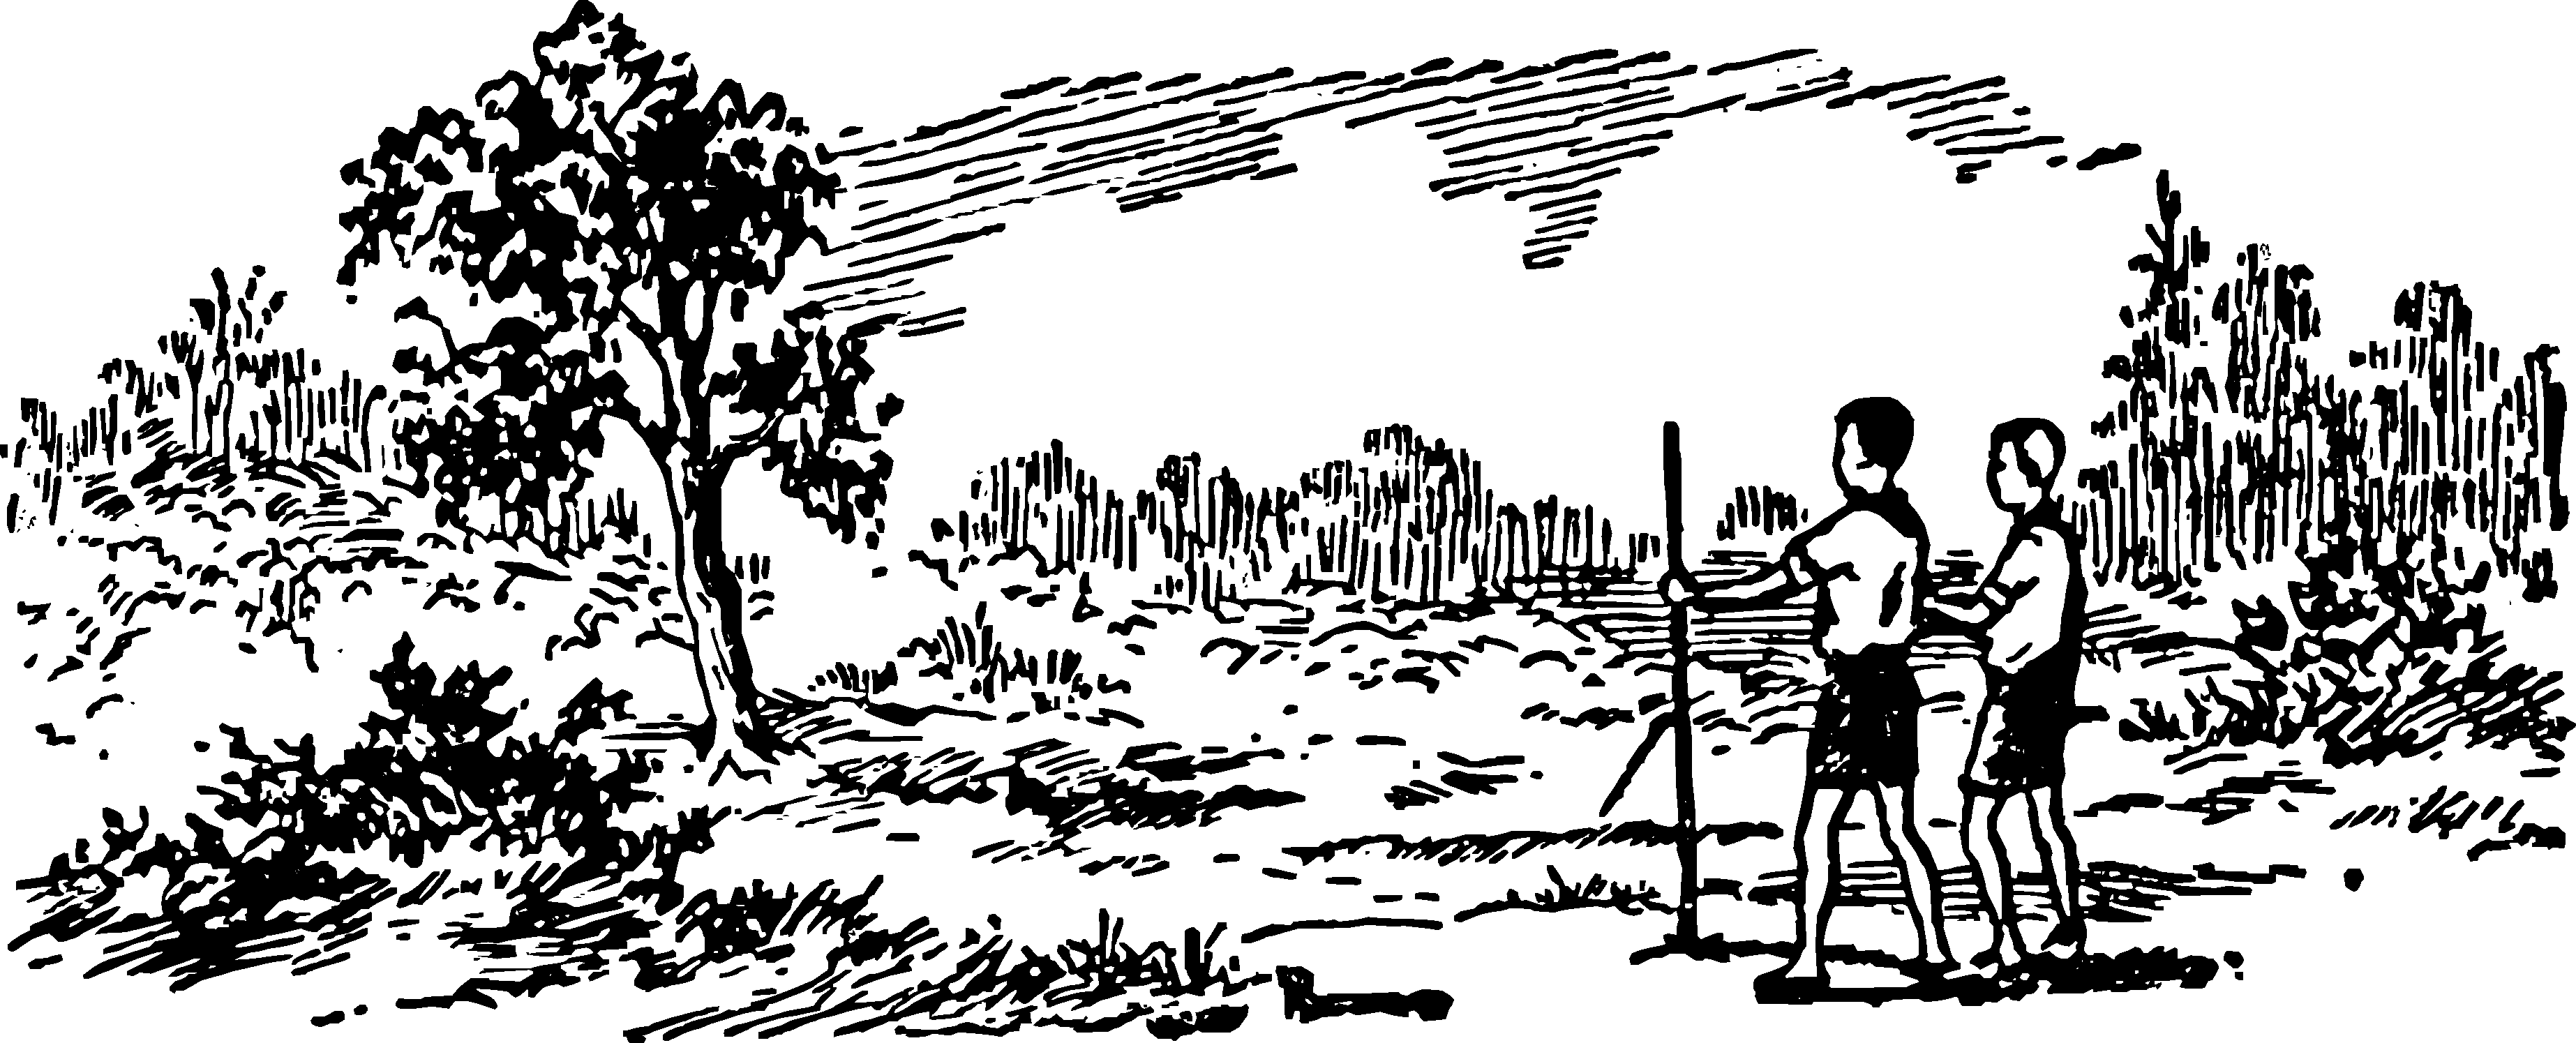
\includegraphics[width=1.2\textwidth]{figures/ch-01/fig-ch-01-head.pdf}\bigskip}

\chapter{Geometry In The Forest}
\label{ch-01}

%\begin{tikzpicture}[remember picture,overlay,shift=(current page.north west)]
%\begin{scope}[x={(current page.north east)},y={(current page.south west)}]
%\node [overlay,remember picture] at (0.5,0.2) {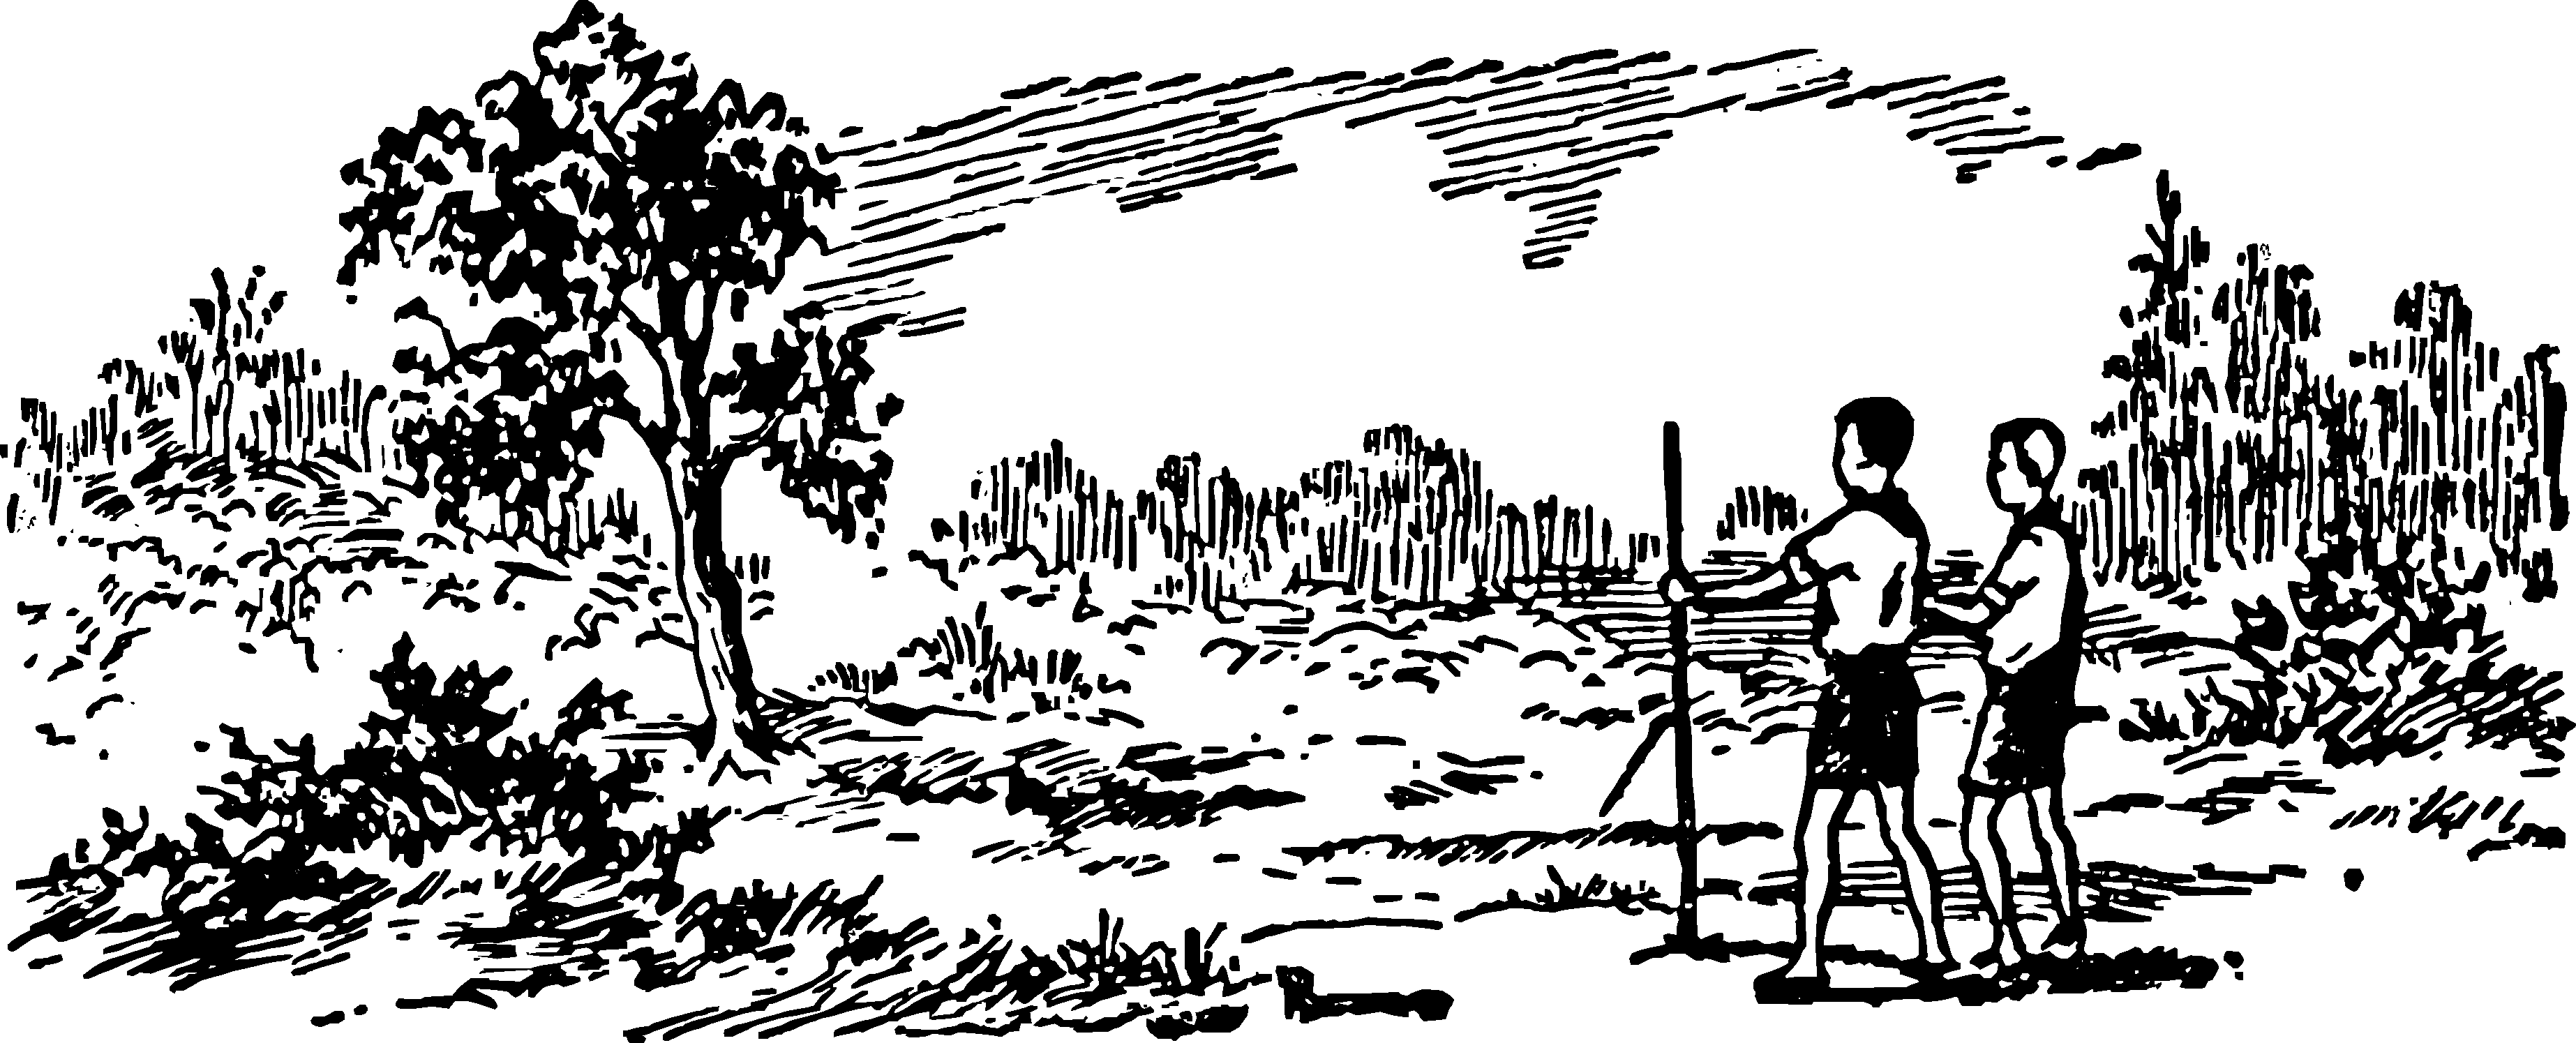
\includegraphics[width=1.2\textwidth]{figures/ch-01/fig-ch-01-head.pdf}};
%\end{scope}
%\end{tikzpicture}

\section{By the length of the shadow}
\label{sec-1.1}

I remember now the amazement with which I looked for the first time, he looked at a gray-haired forester, who, standing near a huge pine tree, measured its height with a small pocket device. When he aimed his square board at the top of the tree, I expected that the old man would now start climbing there with a measuring chain. Instead, he put the device back in his pocket and announced that the measurement was over. I thought it hadn't started yet \ldots{}

I was very young then, and this way of measuring, when a person determines the height of a tree without cutting it down and climbing to the top, was in my eyes something like a small miracle. It was only later, when I was initiated into the rudiments of geometry, that I realised how simple such miracles are performed. There are many different ways to make such measurements using very simple instruments and even without any devices.

The easiest and most ancient way is, without a doubt, the one by which the Greek sage Thales determined the height of the pyramid in Egypt sixth century BC. He took advantage of the pyramid's `shadow'. The priests and the pharaoh, gathered at the foot of the highest pyramid, looked puzzled at the northern newcomer, who guessed the height of the huge structure from the shadow. Thales, says the legend, chose a day and an hour when the length of his own shadow was equal to his height; at this moment, the height of the pyramid should also be equal to the length of the shadow cast by it\sidenote{Of course, the length of the shadow had to be measured from the midpoint of the square base of the pyramid; Thales could directly measure the width of this base.}. This is perhaps the only case when a person benefits from his shadow \ldots{}

The task of the Greek sage now seems childishly simple to us, but let's not forget that we are looking at it from the height of a geometric building erected after Thales. He lived long before Euclid, the author of the wonderful book that taught geometry for two millennia after his death. The truths contained in it, which are now known to every schoolboy, were not yet discovered in the era of Thales. And in order to use the shadow to solve the problem of the height of the pyramid, it was necessary to already know some geometric properties of the triangle, namely the following two (of which Thales himself discovered the first):
\begin{enumerate}
\item that the angles at the base of an isosceles triangle are equal, and vice versa -- that the sides lying opposite the equal angles of the triangle are equal to each other;
\item that the sum of the angles of any triangle (or at least a rectangular one) is equal to two right angles.
\end{enumerate}

Only Thales, armed with this knowledge, had the right to conclude that when his own shadow is equal to his height, the sun's rays meet the flat ground at an angle of half a straight line, and therefore the top of the pyramid, the middle of its base and the end of its shadow should mark an isosceles triangle.

It would seem that this simple method is very convenient to use on a clear sunny day to measure lonely trees whose shadow does not merge with the shadow of neighbouring ones. But in our latitudes it is not as easy as in Egypt to waylay the right moment for this: The sun is low above the horizon, and the shadows are equal to the height of the objects casting them only in the afternoon hours of the summer months. Therefore, the Thales method in this form is not always applicable.

\begin{figure}[h!]
\centering
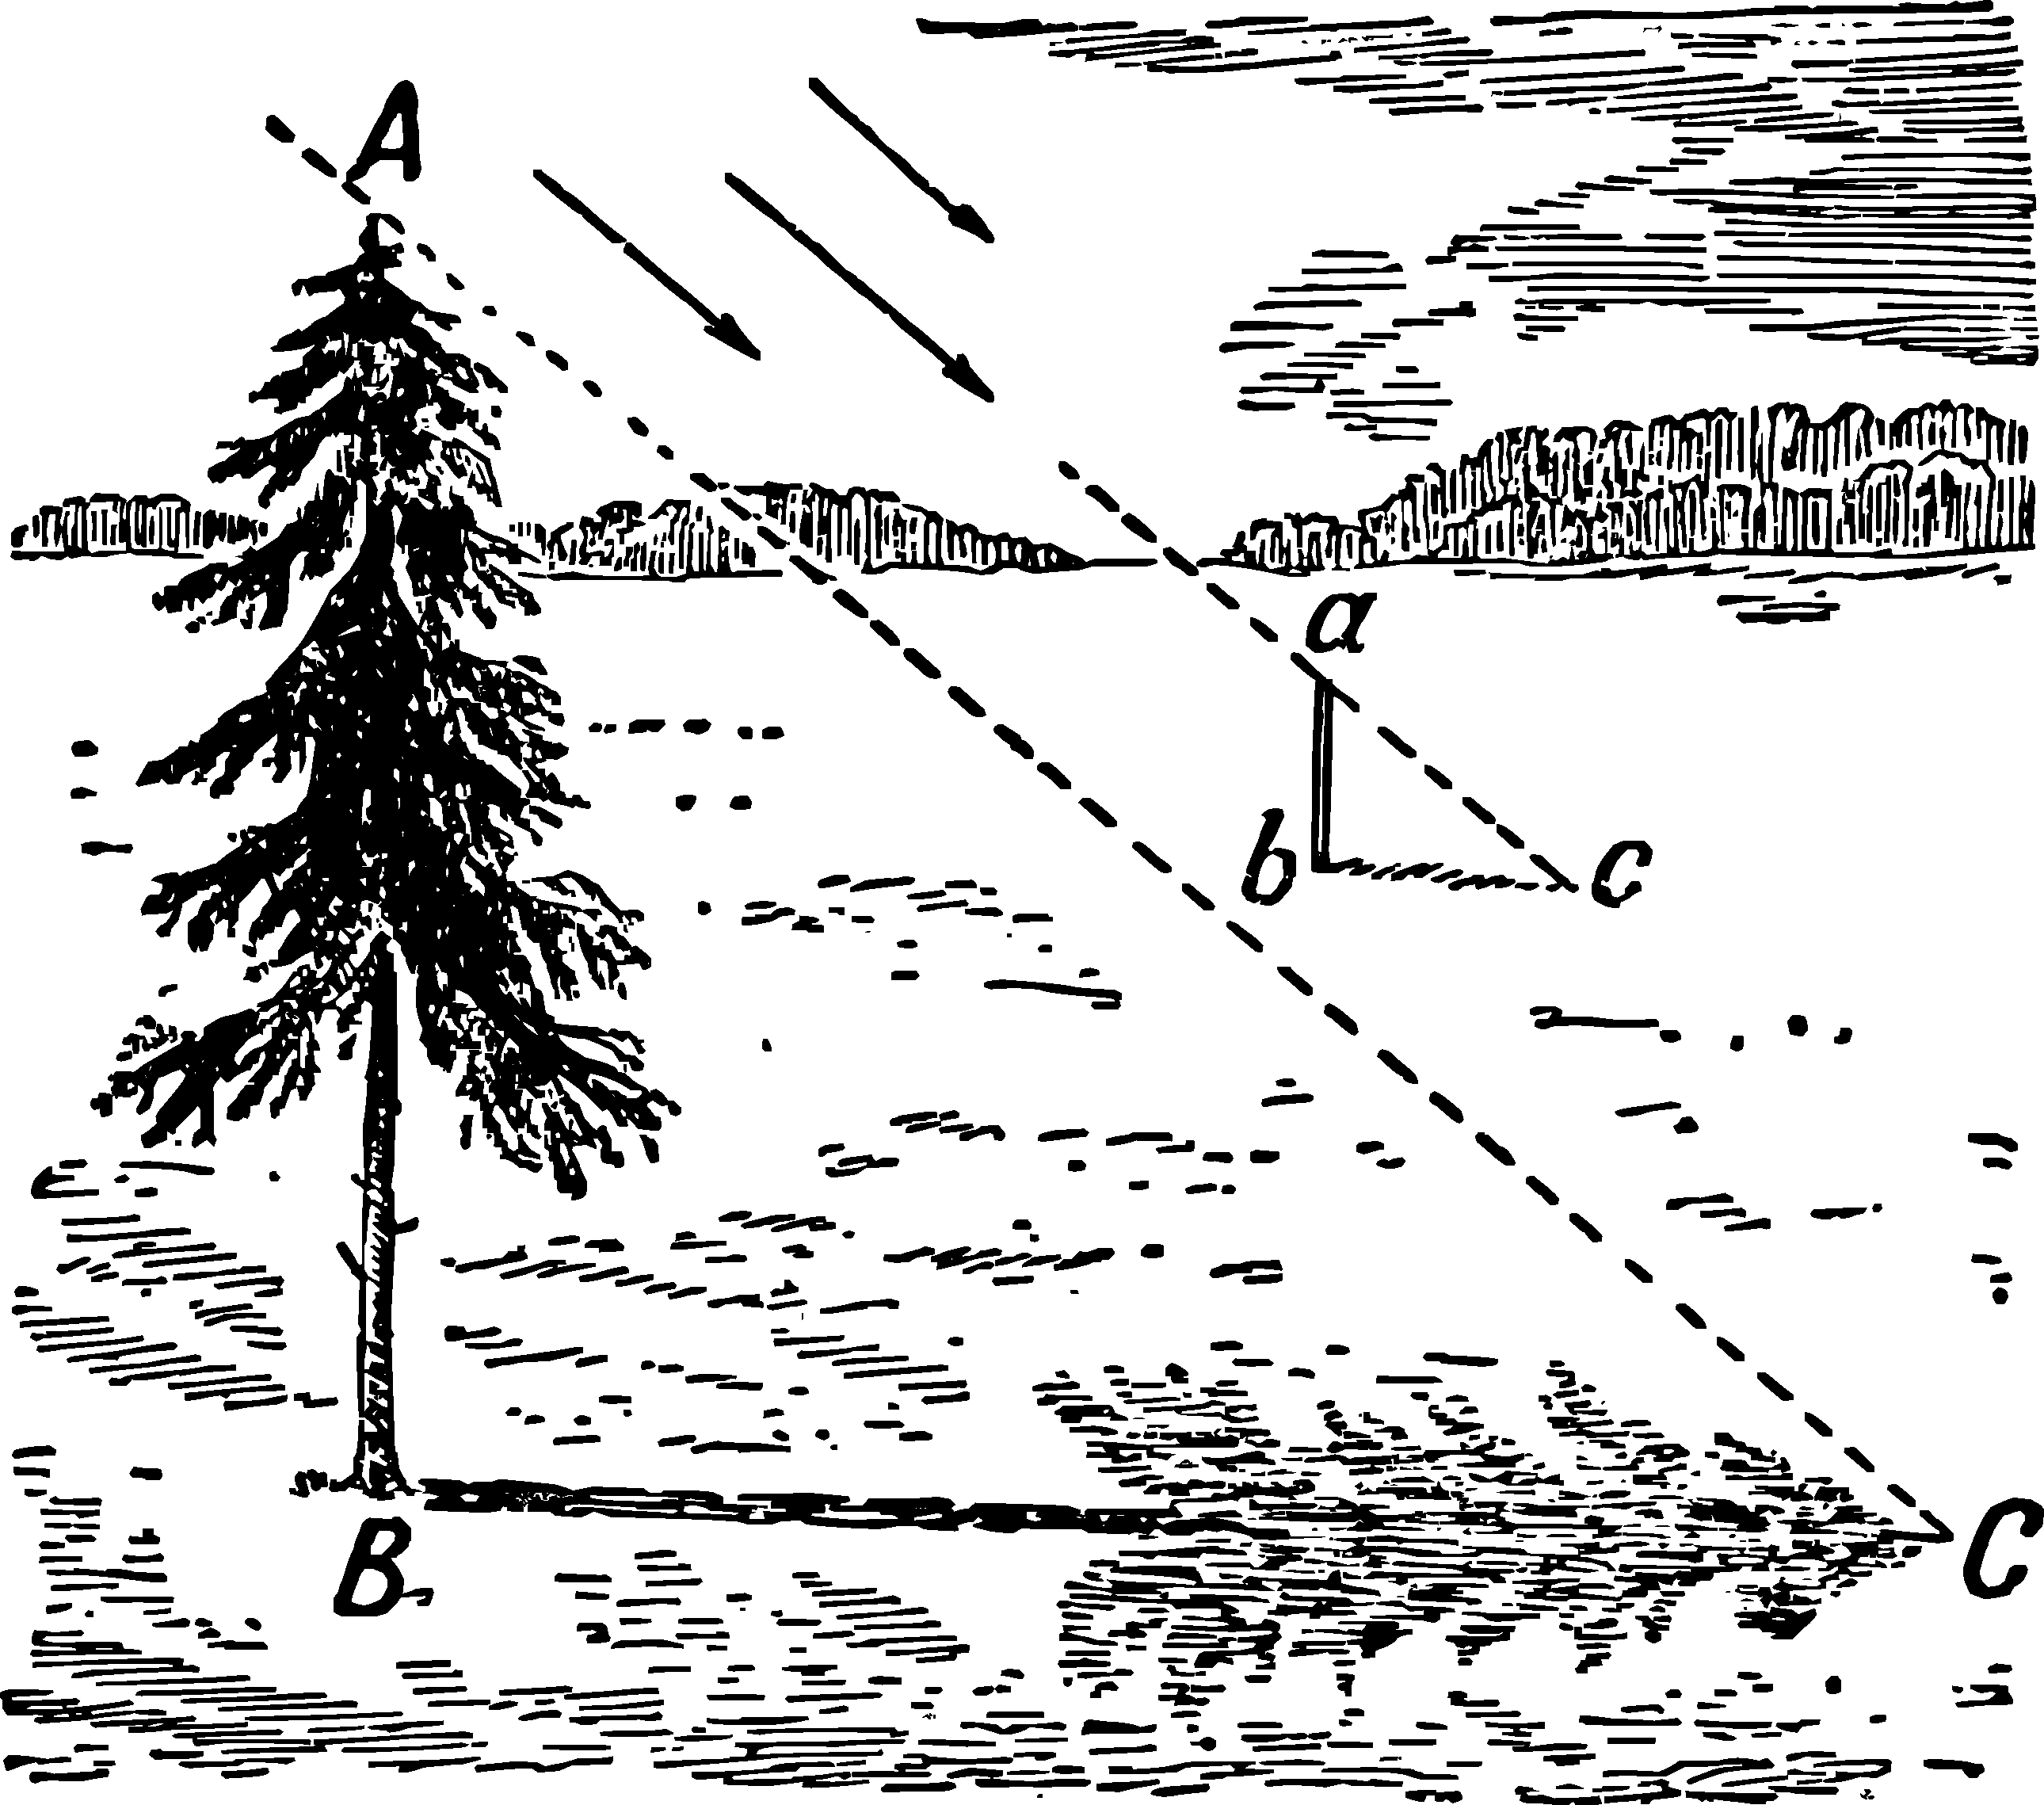
\includegraphics[width=0.9\textwidth]{figures/ch-01/fig-01-01.pdf}
\sidecaption{Measuring the height of a tree by shadow.\label{fig-01-01}}
\end{figure}
It is not difficult, however, to modify this method so that on a sunny day, any shadow can be used, regardless of its length. Additionally, measuring both your own shadow and the shadow of a pole, the desired height is calculated from the proportion (\figr{fig-01-01}):
\begin{equation*}%
AB:ab = BC:bc,
\end{equation*}
meaning the height of the tree is as many times greater than your own height (or the height of the pole) as the shadow of the tree is longer than your shadow (or the shadow of the pole). This naturally follows from the geometric similarity of triangles $ABC$ and $abc$ (based on two angles).

Some readers may object that such an elementary technique does not need a geometric justification at all: is it really unclear even without geometry that how many times is a tree taller, how many times is its shadow longer? However, the matter is not as simple as it seems. Try to apply this rule to shadows cast by the light of a street lamp or lamp -- it will not be justified. In \figr{fig-01-02} you can see that the columns $AB$ are about three times higher than the pedestal $ab$, and the shadow of the column is eight times larger than the shadow of the pedestal $(BC:bc)$. It is impossible to explain why the method is applicable in this case, but not in the other, without geometry.

\begin{figure}[h!]
\centering
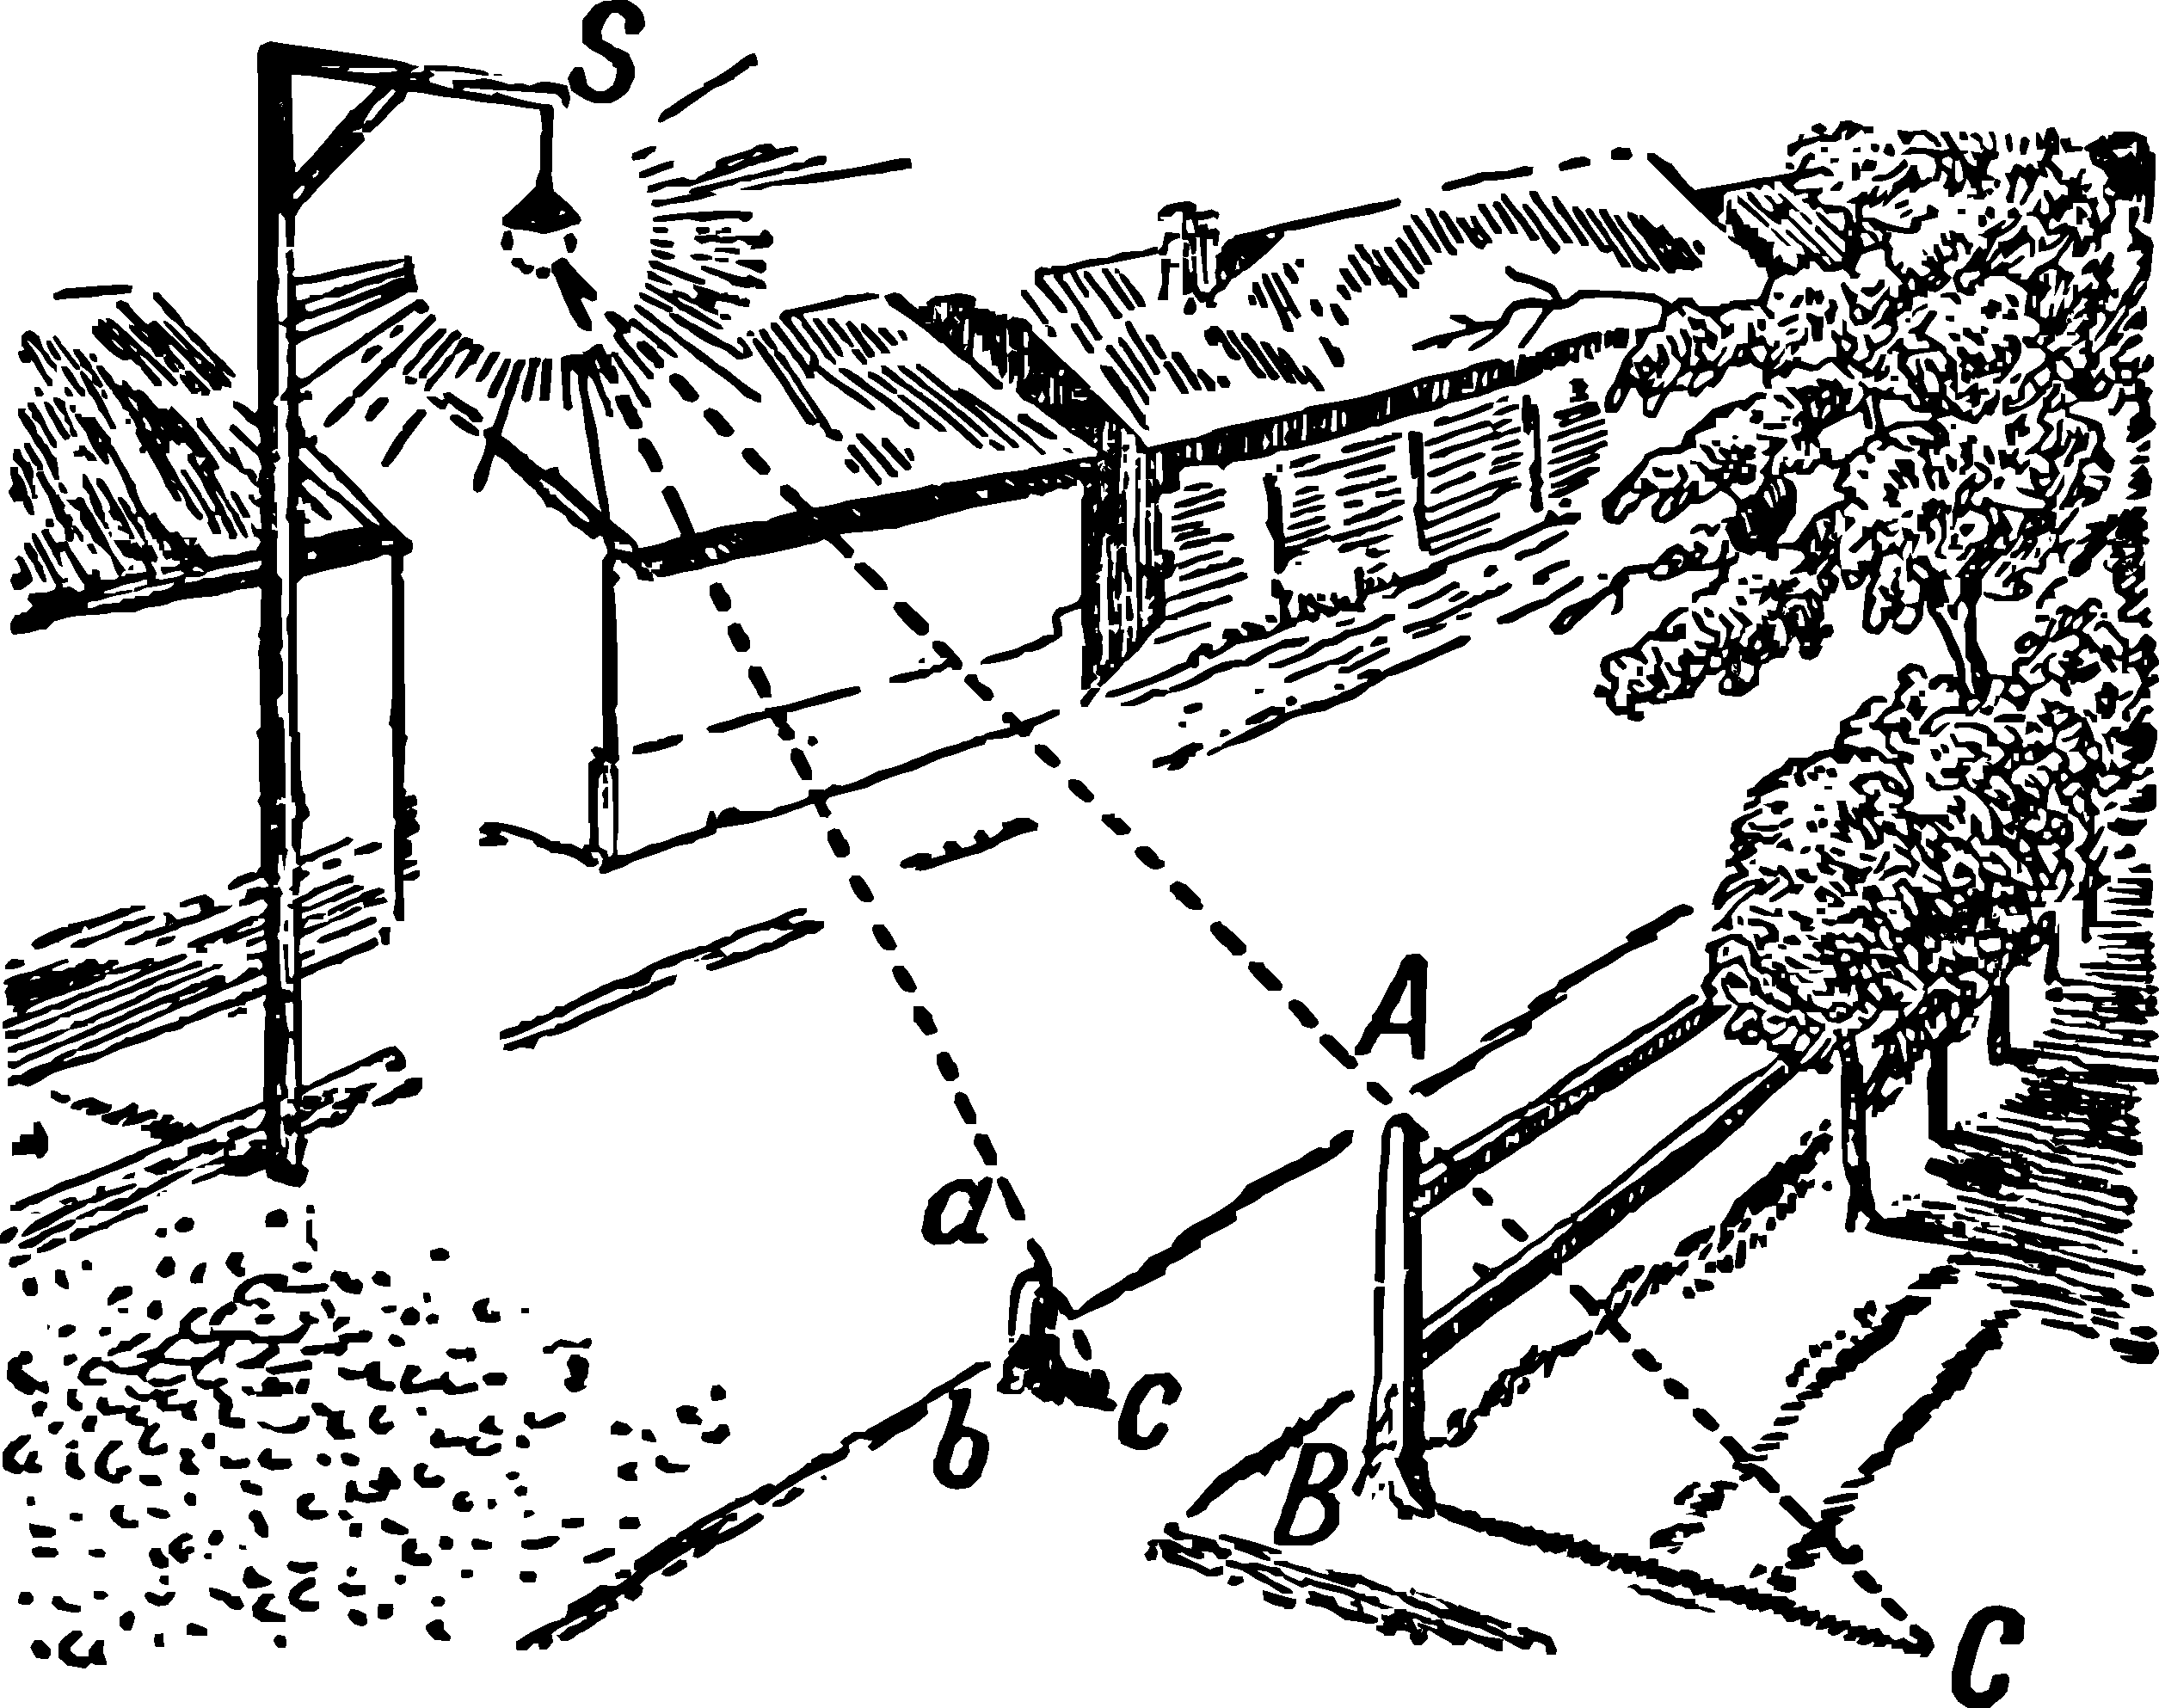
\includegraphics[width=0.9\textwidth]{figures/ch-01/fig-01-02.pdf}
\sidecaption[][0cm]{When such a measurement is impossible. (Is the method applicable for a shadow cast by a streetlamp?)\label{fig-01-02}}
\end{figure}


\ques Let's take a closer look at what the difference is. The essence of the matter boils down. to the fact that the sun's rays are parallel to each other, the rays of the lantern are not parallel. After that, we have the right to consider the rays of the Sun parallel, although they certainly intersect in the place from which they originate.


\ans The rays of the Sun falling on the Earth can be considered parallel because the angle between them is extremely small, almost imperceptible. A simple geometric calculation will convince you of this. Imagine two rays coming from some point of the Sun and falling on the Earth at a distance of, say, one kilo-meter from each other. So, if we put one leg of a compass at this point of the Sun, and with the other we described a circle with a radius equal to the distance from the Sun to the Earth (i.e., with a radius of \SI{150000000}{\kilo\meter}), then an arc of one kilometer in length would appear between our two radii rays. The total length of this gigantic circle would be equal to $2 \pi \times \SI{150000000}{\kilo\meter} = \SI{940000000}{\kilo\meter}$. One degree of it, of course, is 360 times less, i.e. about \SI{2600000}{\kilo\meter}; one arc minute is 60 times less than a degree, i.e. equal to \SI{43000}{\kilo\meter}, and one arc second is another 60 times less, i.e. \SI{720}{\kilo\meter}. But our arc is only \SI{1}{\kilo\meter} in length, so it corresponds to an angle of $1/720 \approx \ang{;;0.00138}$ seconds. This angle is elusive even for the most accurate astronomical instruments; therefore, in practise we can consider the rays of the Sun falling on the Earth as parallel lines.\sidenote{Another thing is the rays directed from some point of the Sun to the ends of the earth's diameter; the angle between them is large enough to measure (about \ang{;;17}); the definition of this angle gave astronomers one of the means to establish how great the distance from the Earth to the Sun is.}

Trying to apply the method of shadows in practise, you will immediately be convinced, however, of its unreliability. Shadows are not delimited so clearly that measuring their length can be done quite accurately. Each shadow cast by the light of the Sun has an indistinctly outlined grey border of penumbra, which gives the border of the shadow uncertainty. This is because the Sun is not a point, but a large luminous body emitting rays from many points. \figr{fig-01-03} illustrates why, as a result of this, the shadow of tree $AB$ also has an additional component in the form of half-shadow $CD$, gradually fading away.

\begin{figure}[h!]
\centering
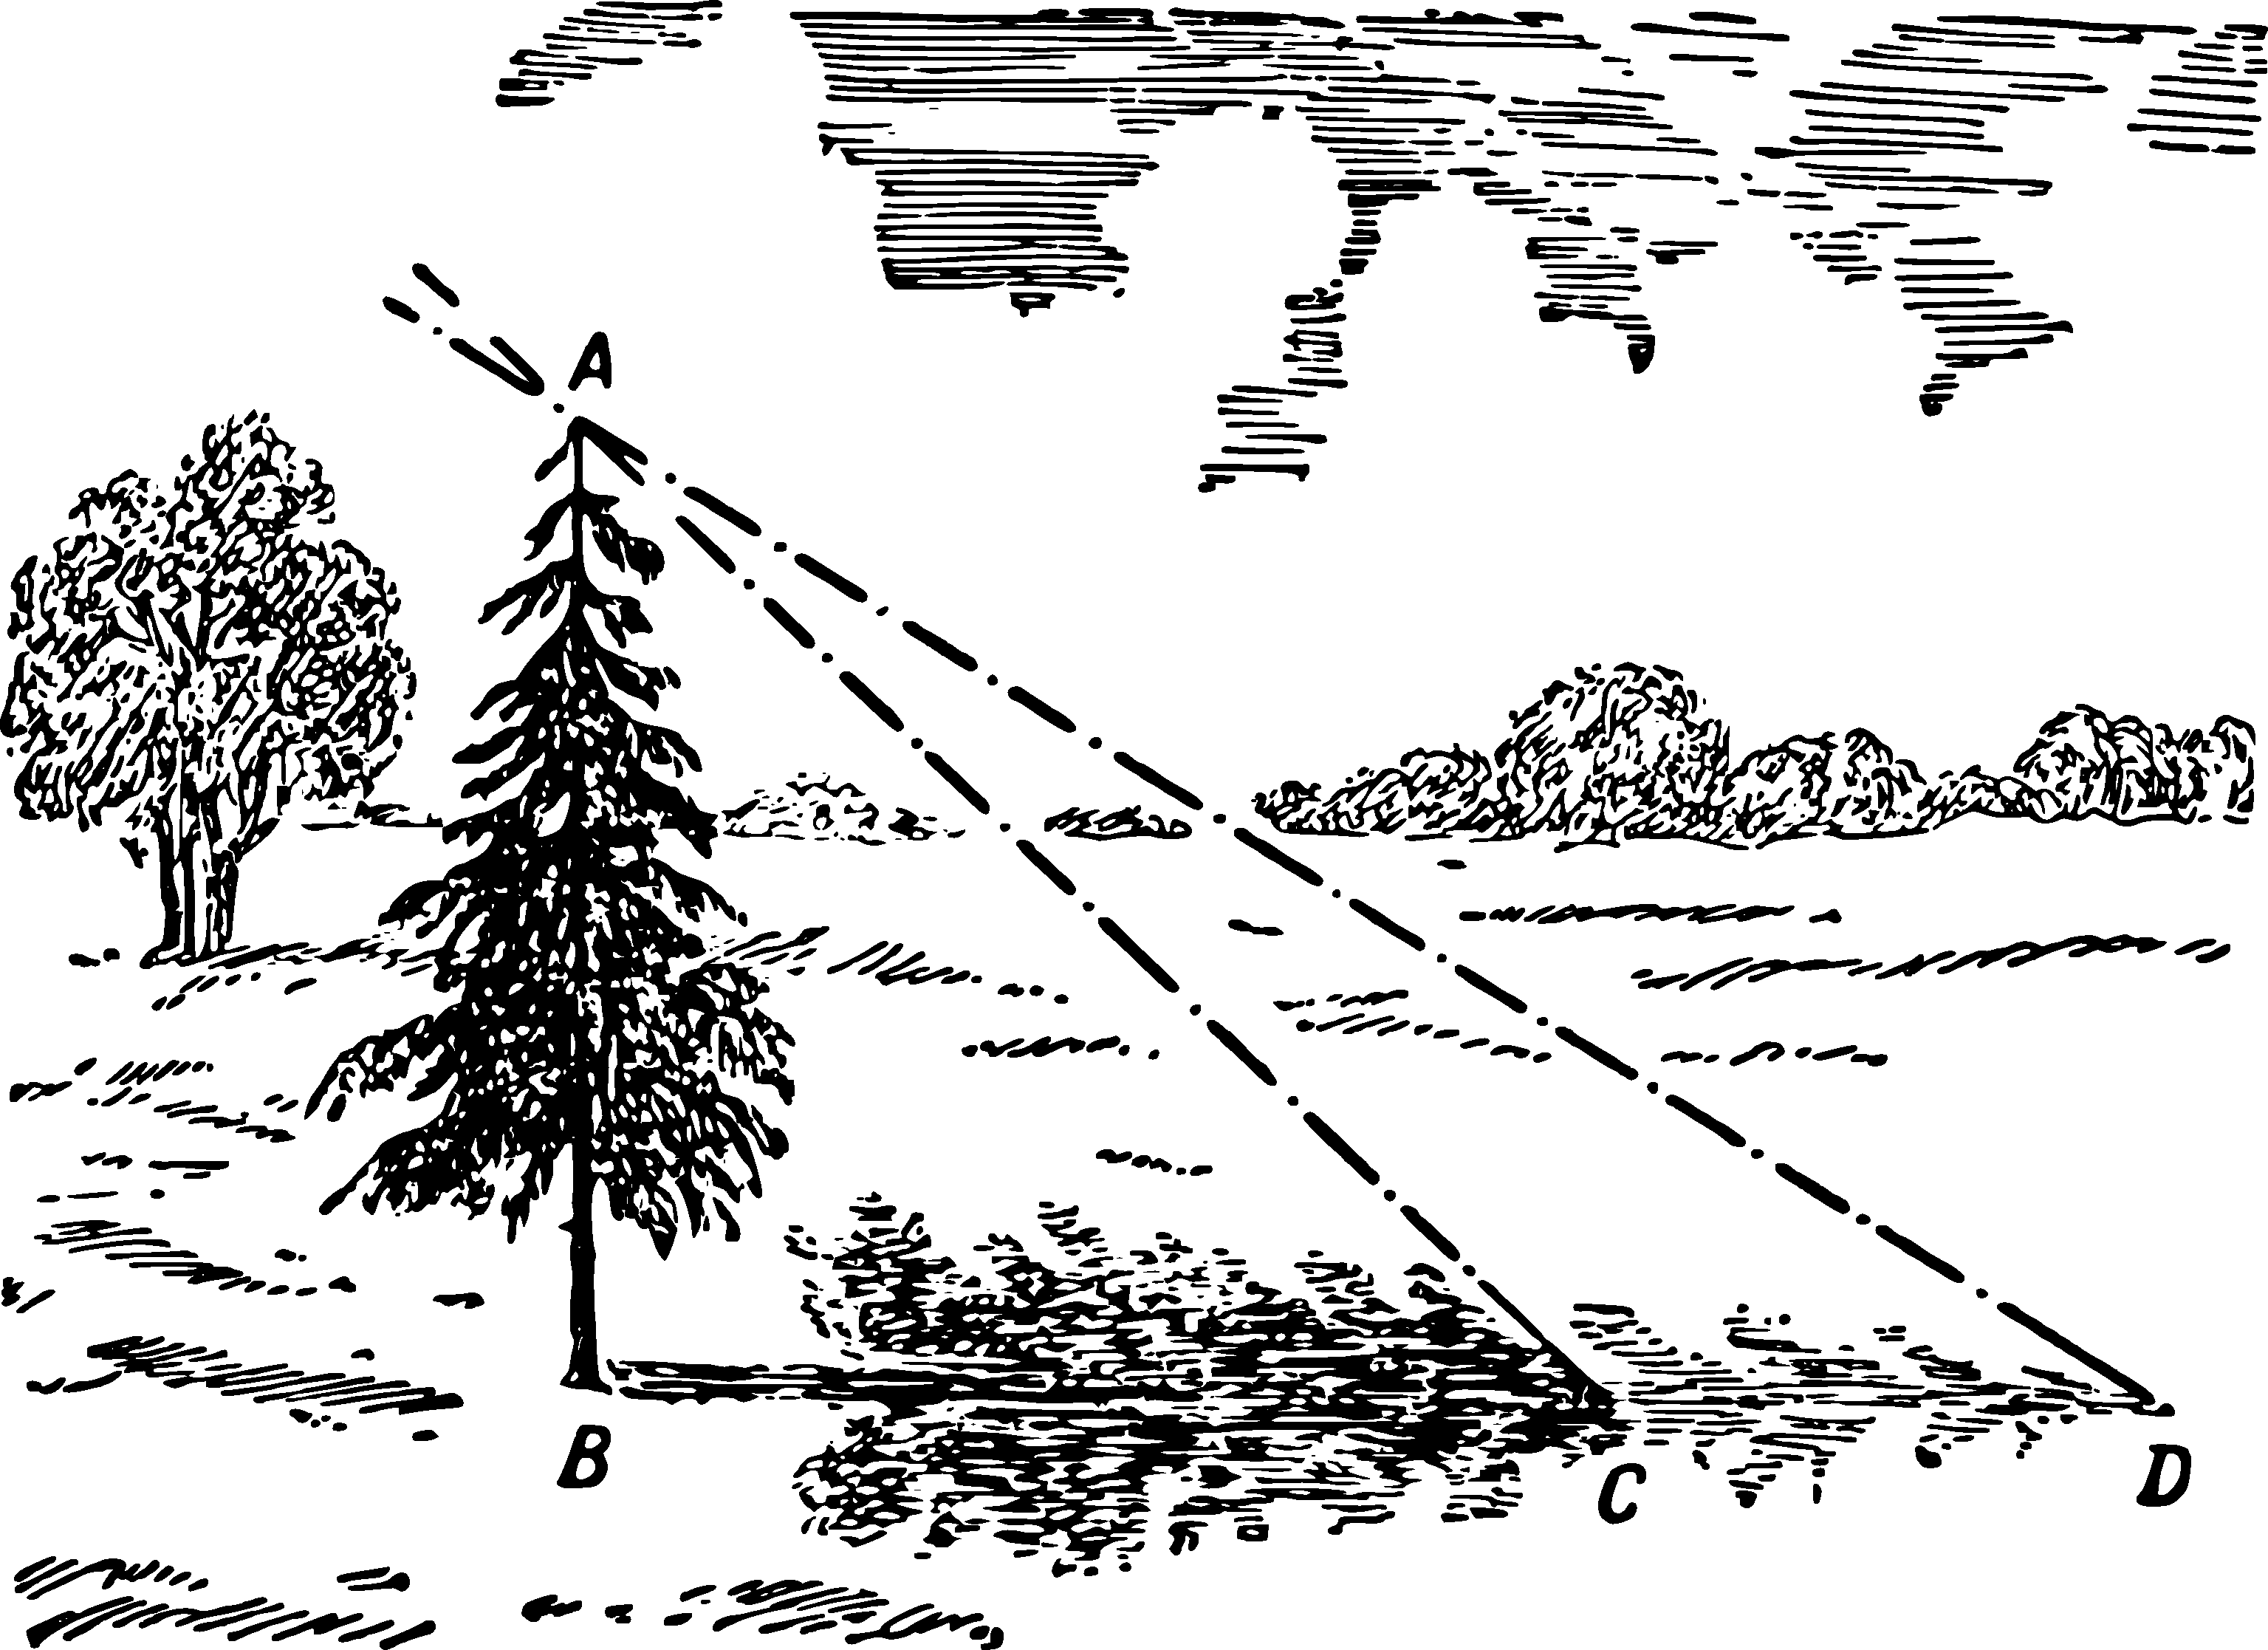
\includegraphics[width=0.9\textwidth]{figures/ch-01/fig-01-03.pdf}
\sidecaption{How penumbra is formed.\label{fig-01-03}}
\end{figure}


The angle of the $CAD$ between the extreme boundaries of the penumbra is equal to the angle at which we always see the solar disk, i.e. half a degree. The error resulting from the fact that both shadows are not measured quite accurately can reach 5\% or more when the Sun is not too low. This error is added to other unavoidable errors -- from uneven soil, etc. -- and makes the final result little reliable. In mountainous terrain, for example, this method is completely inapplicable.

\clearpage

\section{Two More Methods}
\label{sec-1.2}

It is entirely possible to measure height without relying on shadows. There are many methods; let's start with two simple ones.

Firstly, we can utilise the properties of an isosceles right triangle. For this purpose, we can make use of a very simple tool, which can be easily crafted from a piece of board and three pins. On a board of any shape, even a piece of bark with a flat side, mark three points to form the vertices of a right triangle -- and insert a pin at each point (see \figr{fig-01-04}). Suppose you don't have a drafting triangle to construct a right angle, nor a compass to mark equal sides. In that case, fold any piece of paper once, and then fold it again across the first fold so that both parts of the first fold coincide -- and you'll obtain a right angle. The same piece of paper can be used instead of a compass to measure equal distances.

\begin{figure}[h!]
\centering
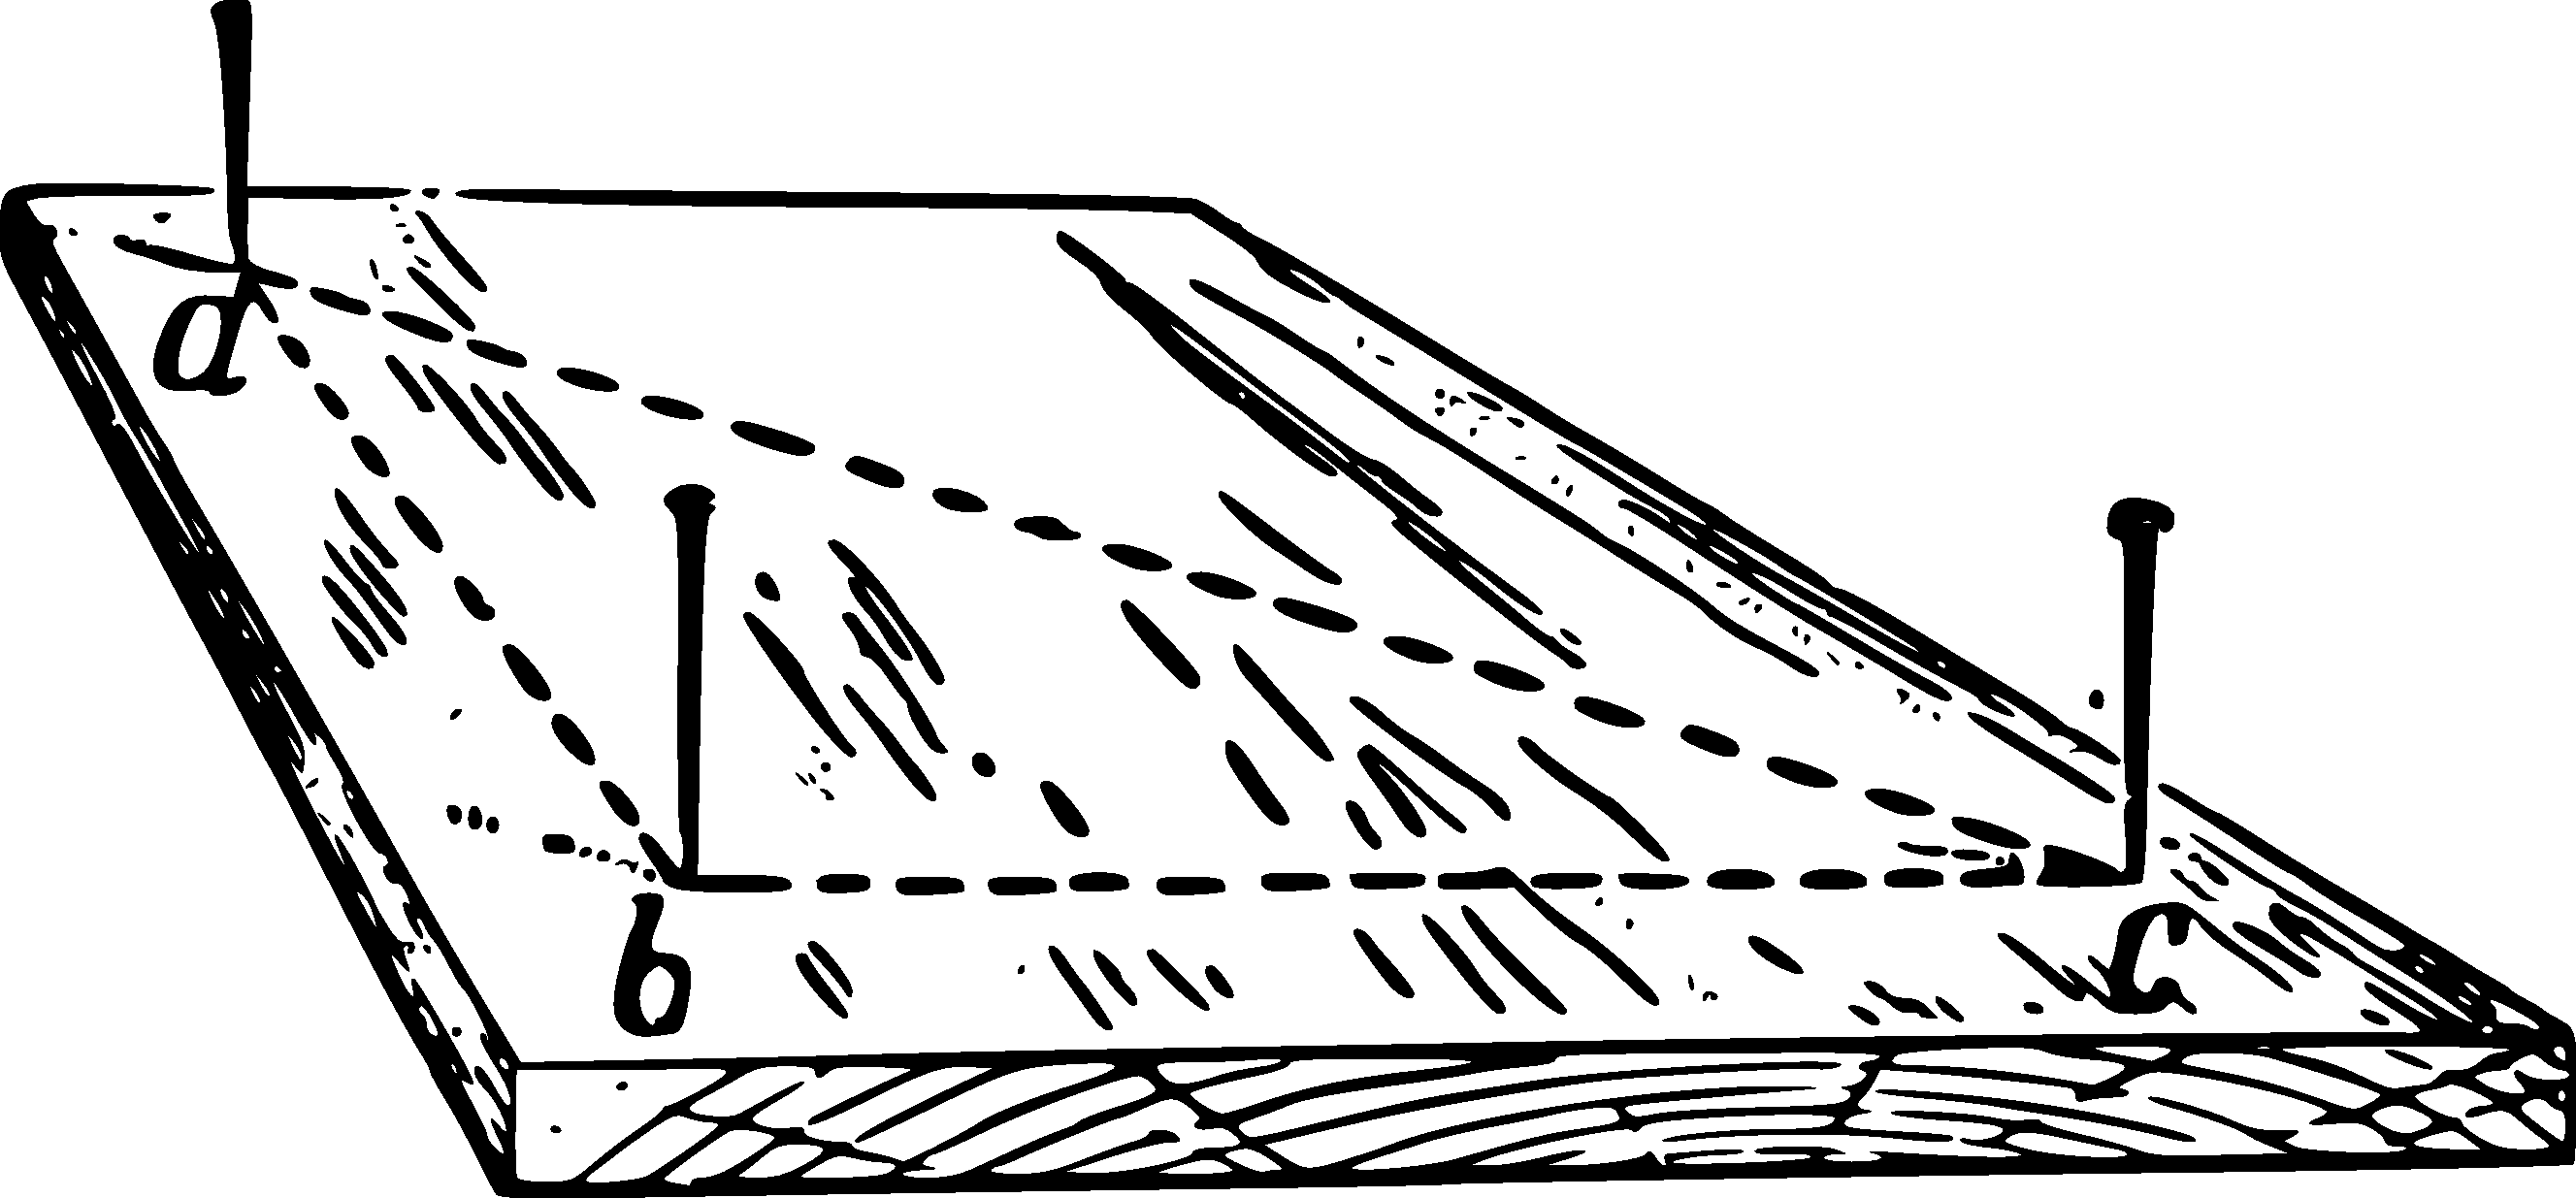
\includegraphics[width=0.6\textwidth]{figures/ch-01/fig-01-04.pdf}
\sidecaption{Pin height measuring device.\label{fig-01-04}}
\end{figure}


As you can see, the tool can be entirely crafted in a makeshift environment.

If you don't have a drafting triangle on hand to construct a right angle, nor a compass to mark equal sides, then simply fold any scrap of paper once, and then fold it again across the first fold so that both parts of the first fold coincide—and you'll obtain a right angle. The same piece of paper can be used instead of a compass to measure equal distances.

As you can see, the tool can be entirely crafted in a makeshift environment.

\begin{figure}[h!]
\centering
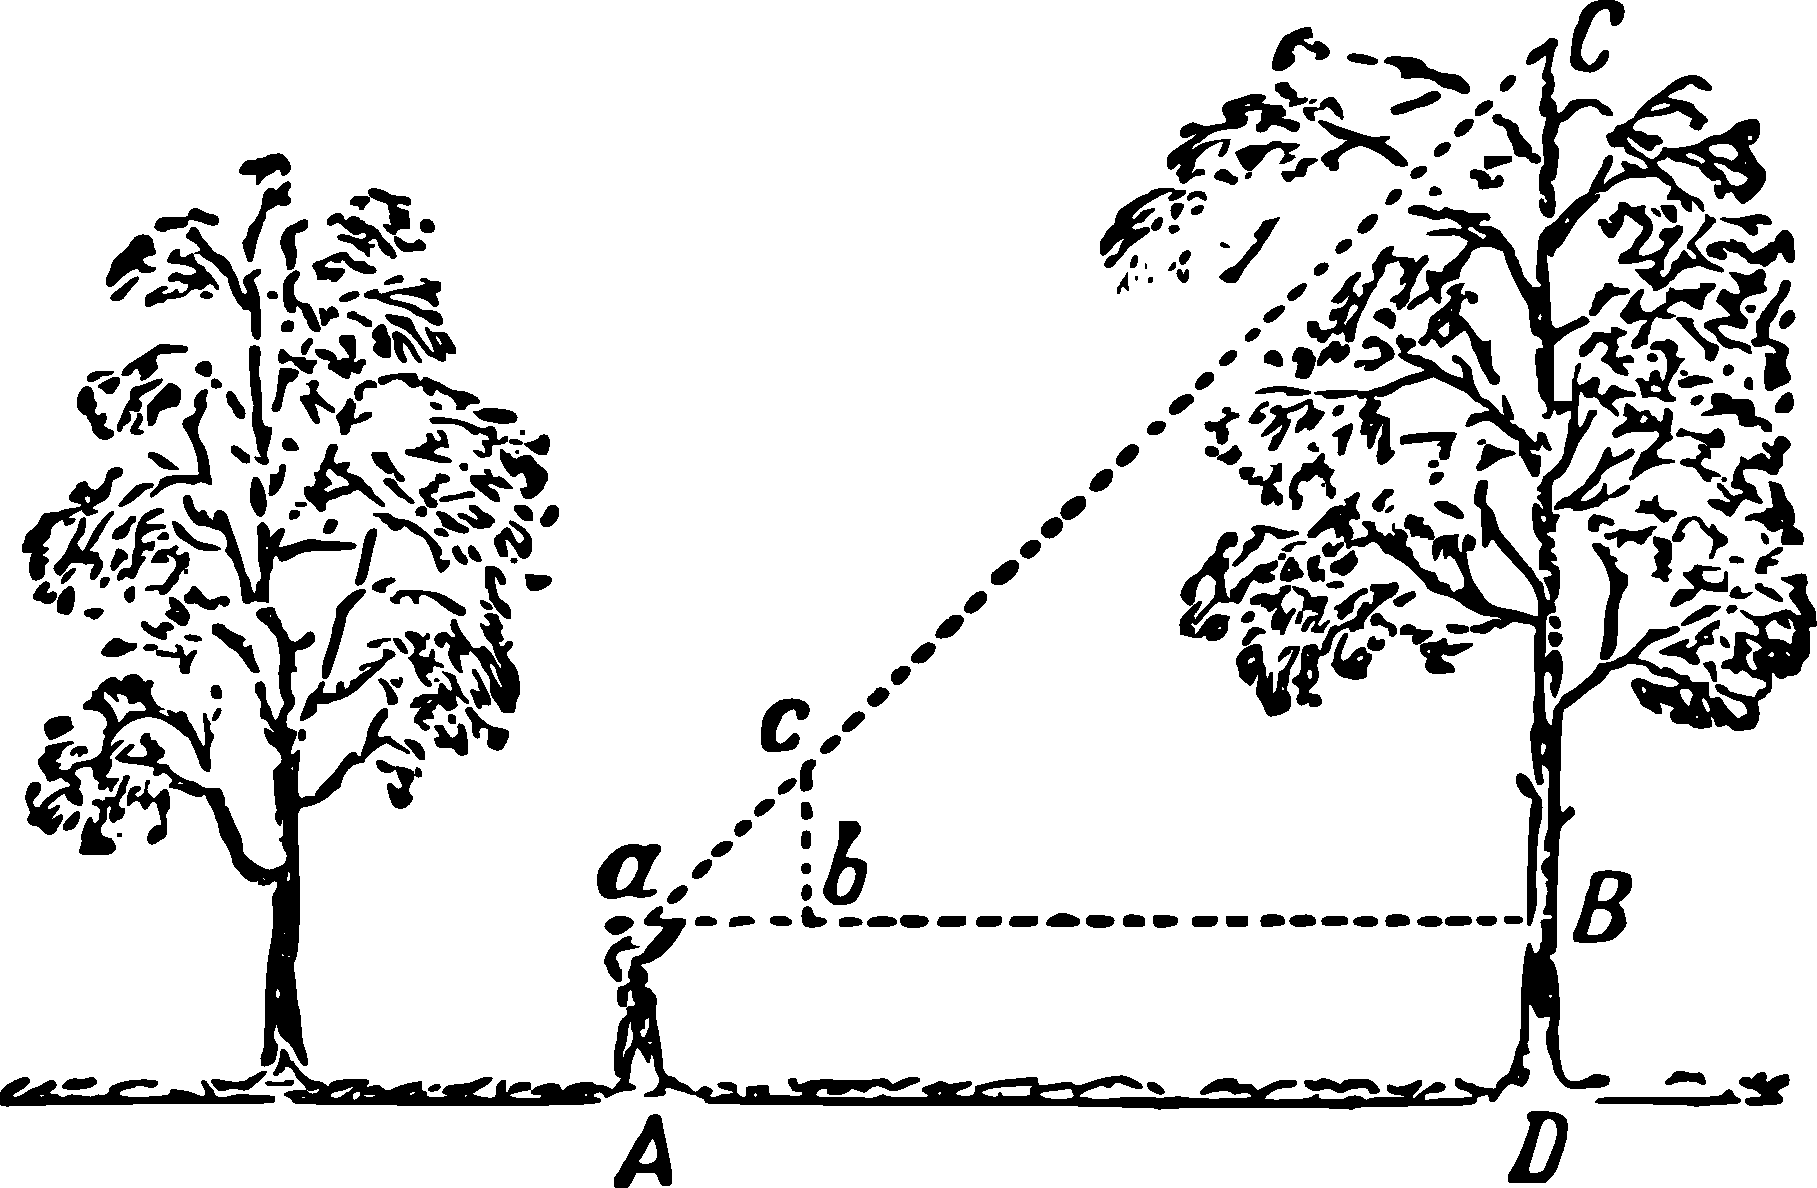
\includegraphics[width=0.9\textwidth]{figures/ch-01/fig-01-05.pdf}
\sidecaption{The scheme of application of the pin device.\label{fig-01-05}}
\end{figure}

Handling it is no more difficult than crafting it. Stepping away from the tree being measured, hold the tool so that one of the legs of the triangle is perpendicular. You can use a string or a weight tied to the top pin. Approaching or moving away from the tree, you will always find a spot $A$ (see \figr{fig-01-05}), from which, looking at pins $a$ and $c$, you will see that they cover the top $C$ of the tree: this means that the extension of the hypotenuse $ac$ passes through point $C$. Then, obviously, the distance $aB$ is equal to $CB$, since angle $a = \ang{45}$. 

Consequently, by measuring distance $aB$ (or, at another location, distance $AD$) and adding $BD$ to it, i.e., the elevation of point $a$ above the ground, you will obtain the desired height of the tree.

\begin{figure}[h!]
\centering
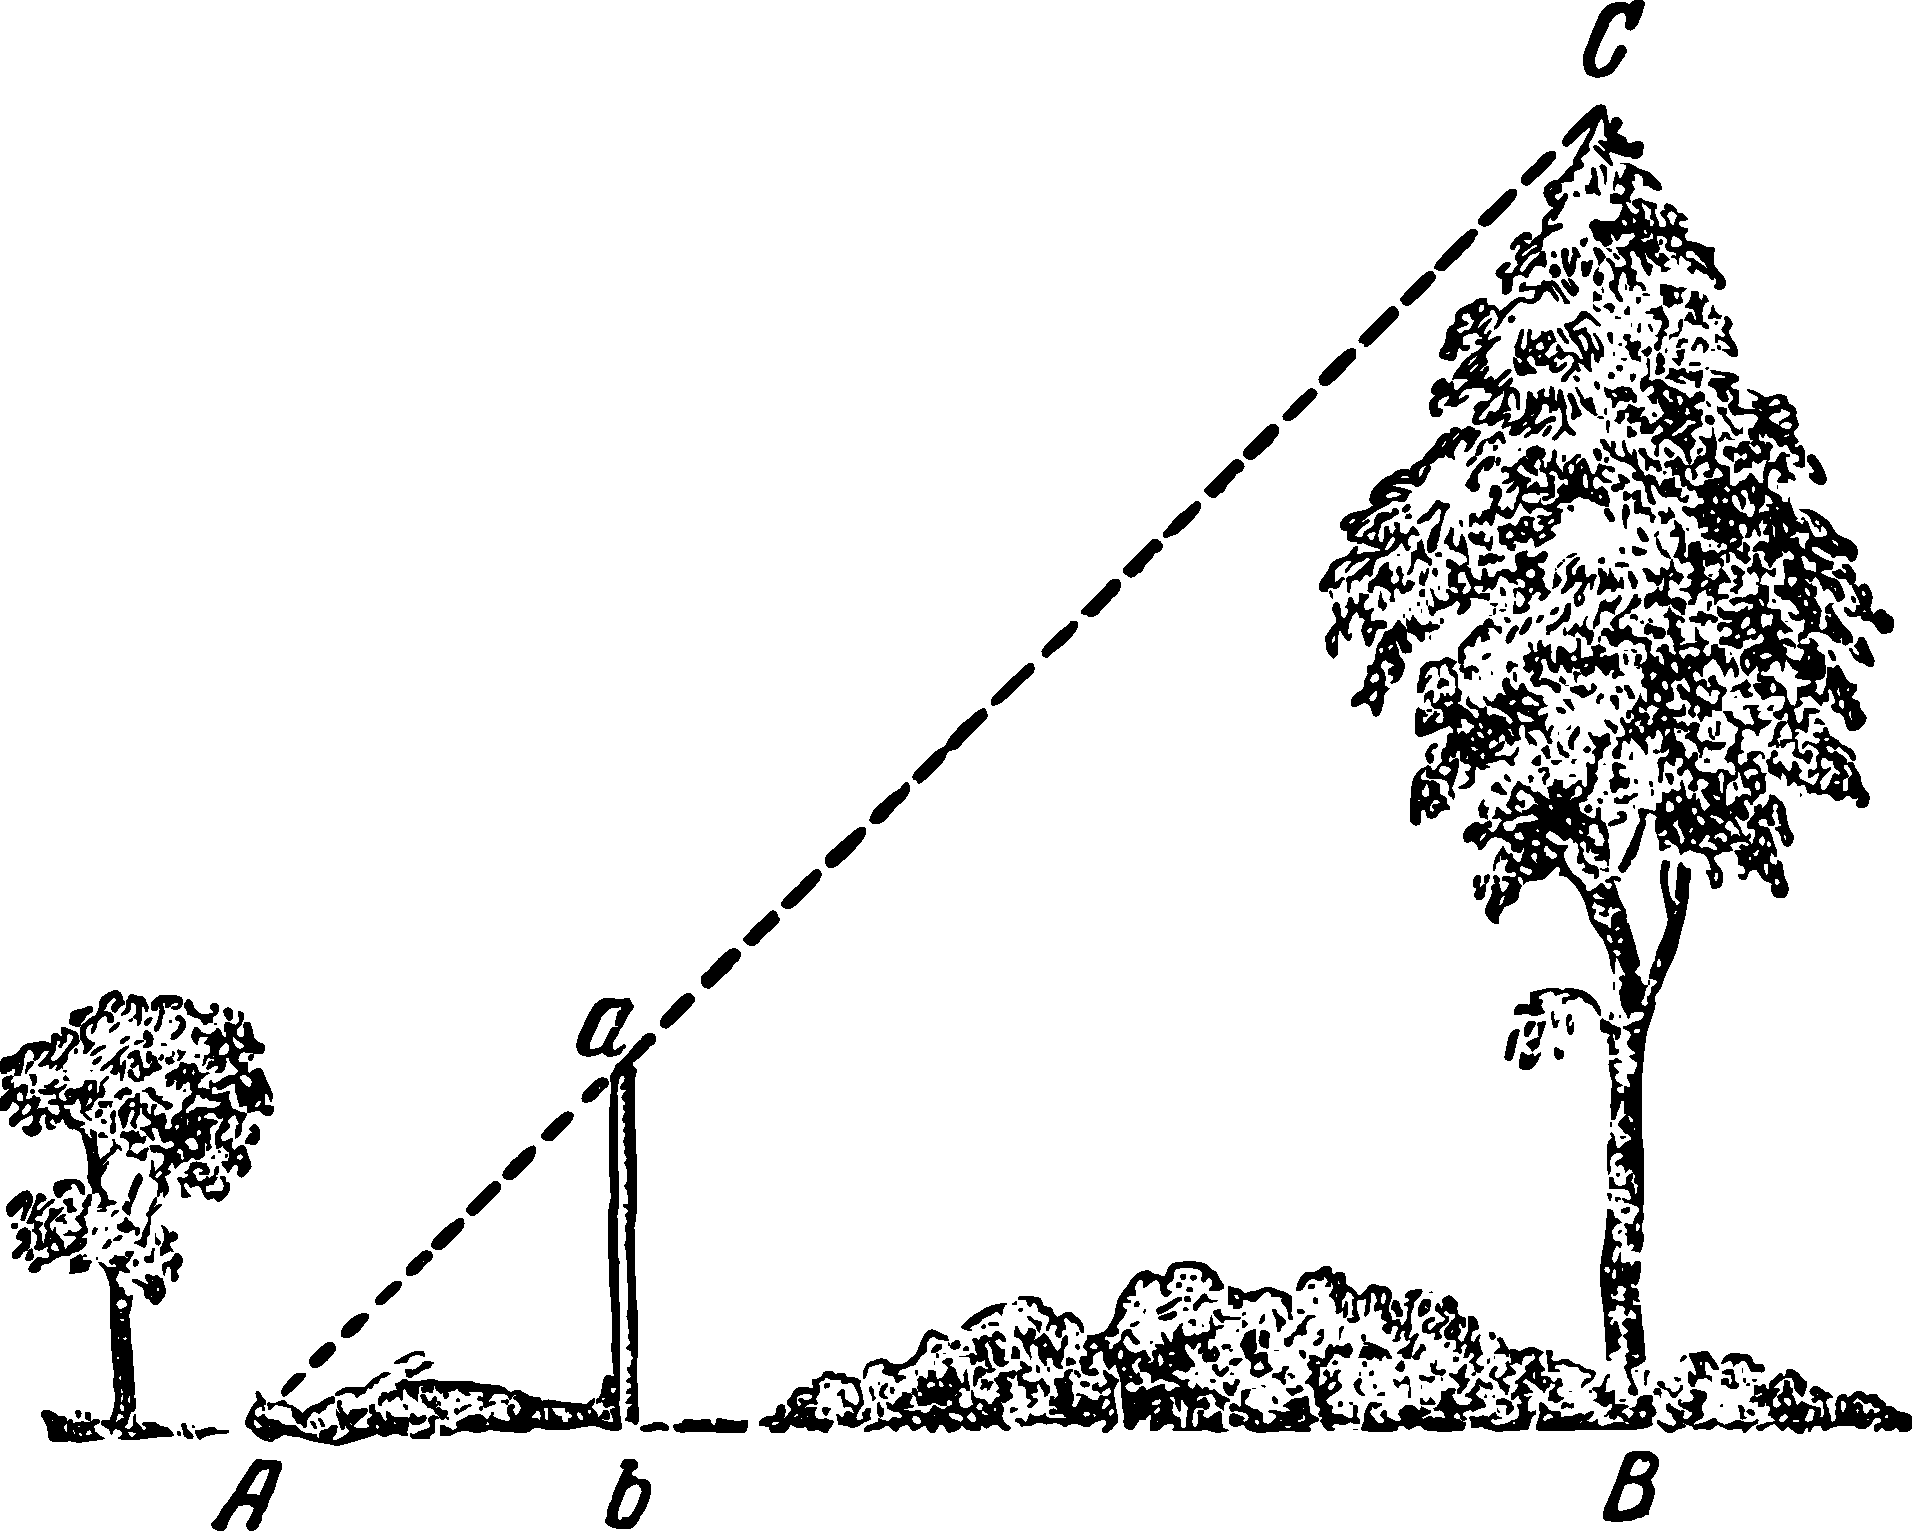
\includegraphics[width=0.9\textwidth]{figures/ch-01/fig-01-06.pdf}
\sidecaption{Another way to determine the height.\label{fig-01-06}}
\end{figure}

Another method does not even require a pin device. Here you need a pole, which you will have to insert vertically into the ground so that the protruding part is exactly at your height. The location for the pole must be chosen so that, lying down as shown in \figr{fig-01-06}, you see the top of the tree in a straight line with the upper point of the pole. Since triangle $Aba$ is isosceles and right-angled, angle $A = \ang{45}$, and therefore $AB$ equals $BC$, i.e., the desired height of the tree.



\section{The Method of Jules Verne}
\label{sec-1.3}

The next, also quite simple, method for measuring tall objects is vividly described by Jules Verne in his famous novel \emph{The Mysterious Island.}

``Today we need to measure the height of the Far View platform,'' said the engineer.

``Will you need a tool for that?'' asked Herbert.

``No, we won't. We'll proceed somewhat differently, resorting to a somewhat simpler and more accurate method.''

The young man, eager to learn as much as possible, followed the engineer, who descended from the granite wall to the rocky shore.

Taking a straight pole, twelve feet long, the engineer measured it as precisely as possible, comparing it to his own height, which he knew well. Meanwhile, Herbert held a plumb bob given to him by the engineer: just a stone attached to the end of a rope.

Not reaching five hundred feet from the granite wall, which rose vertically, the engineer drove the pole two feet into the sand and firmly secured it, placing it vertically with the help of the plumb bob.

\begin{figure}[h!]
\centering
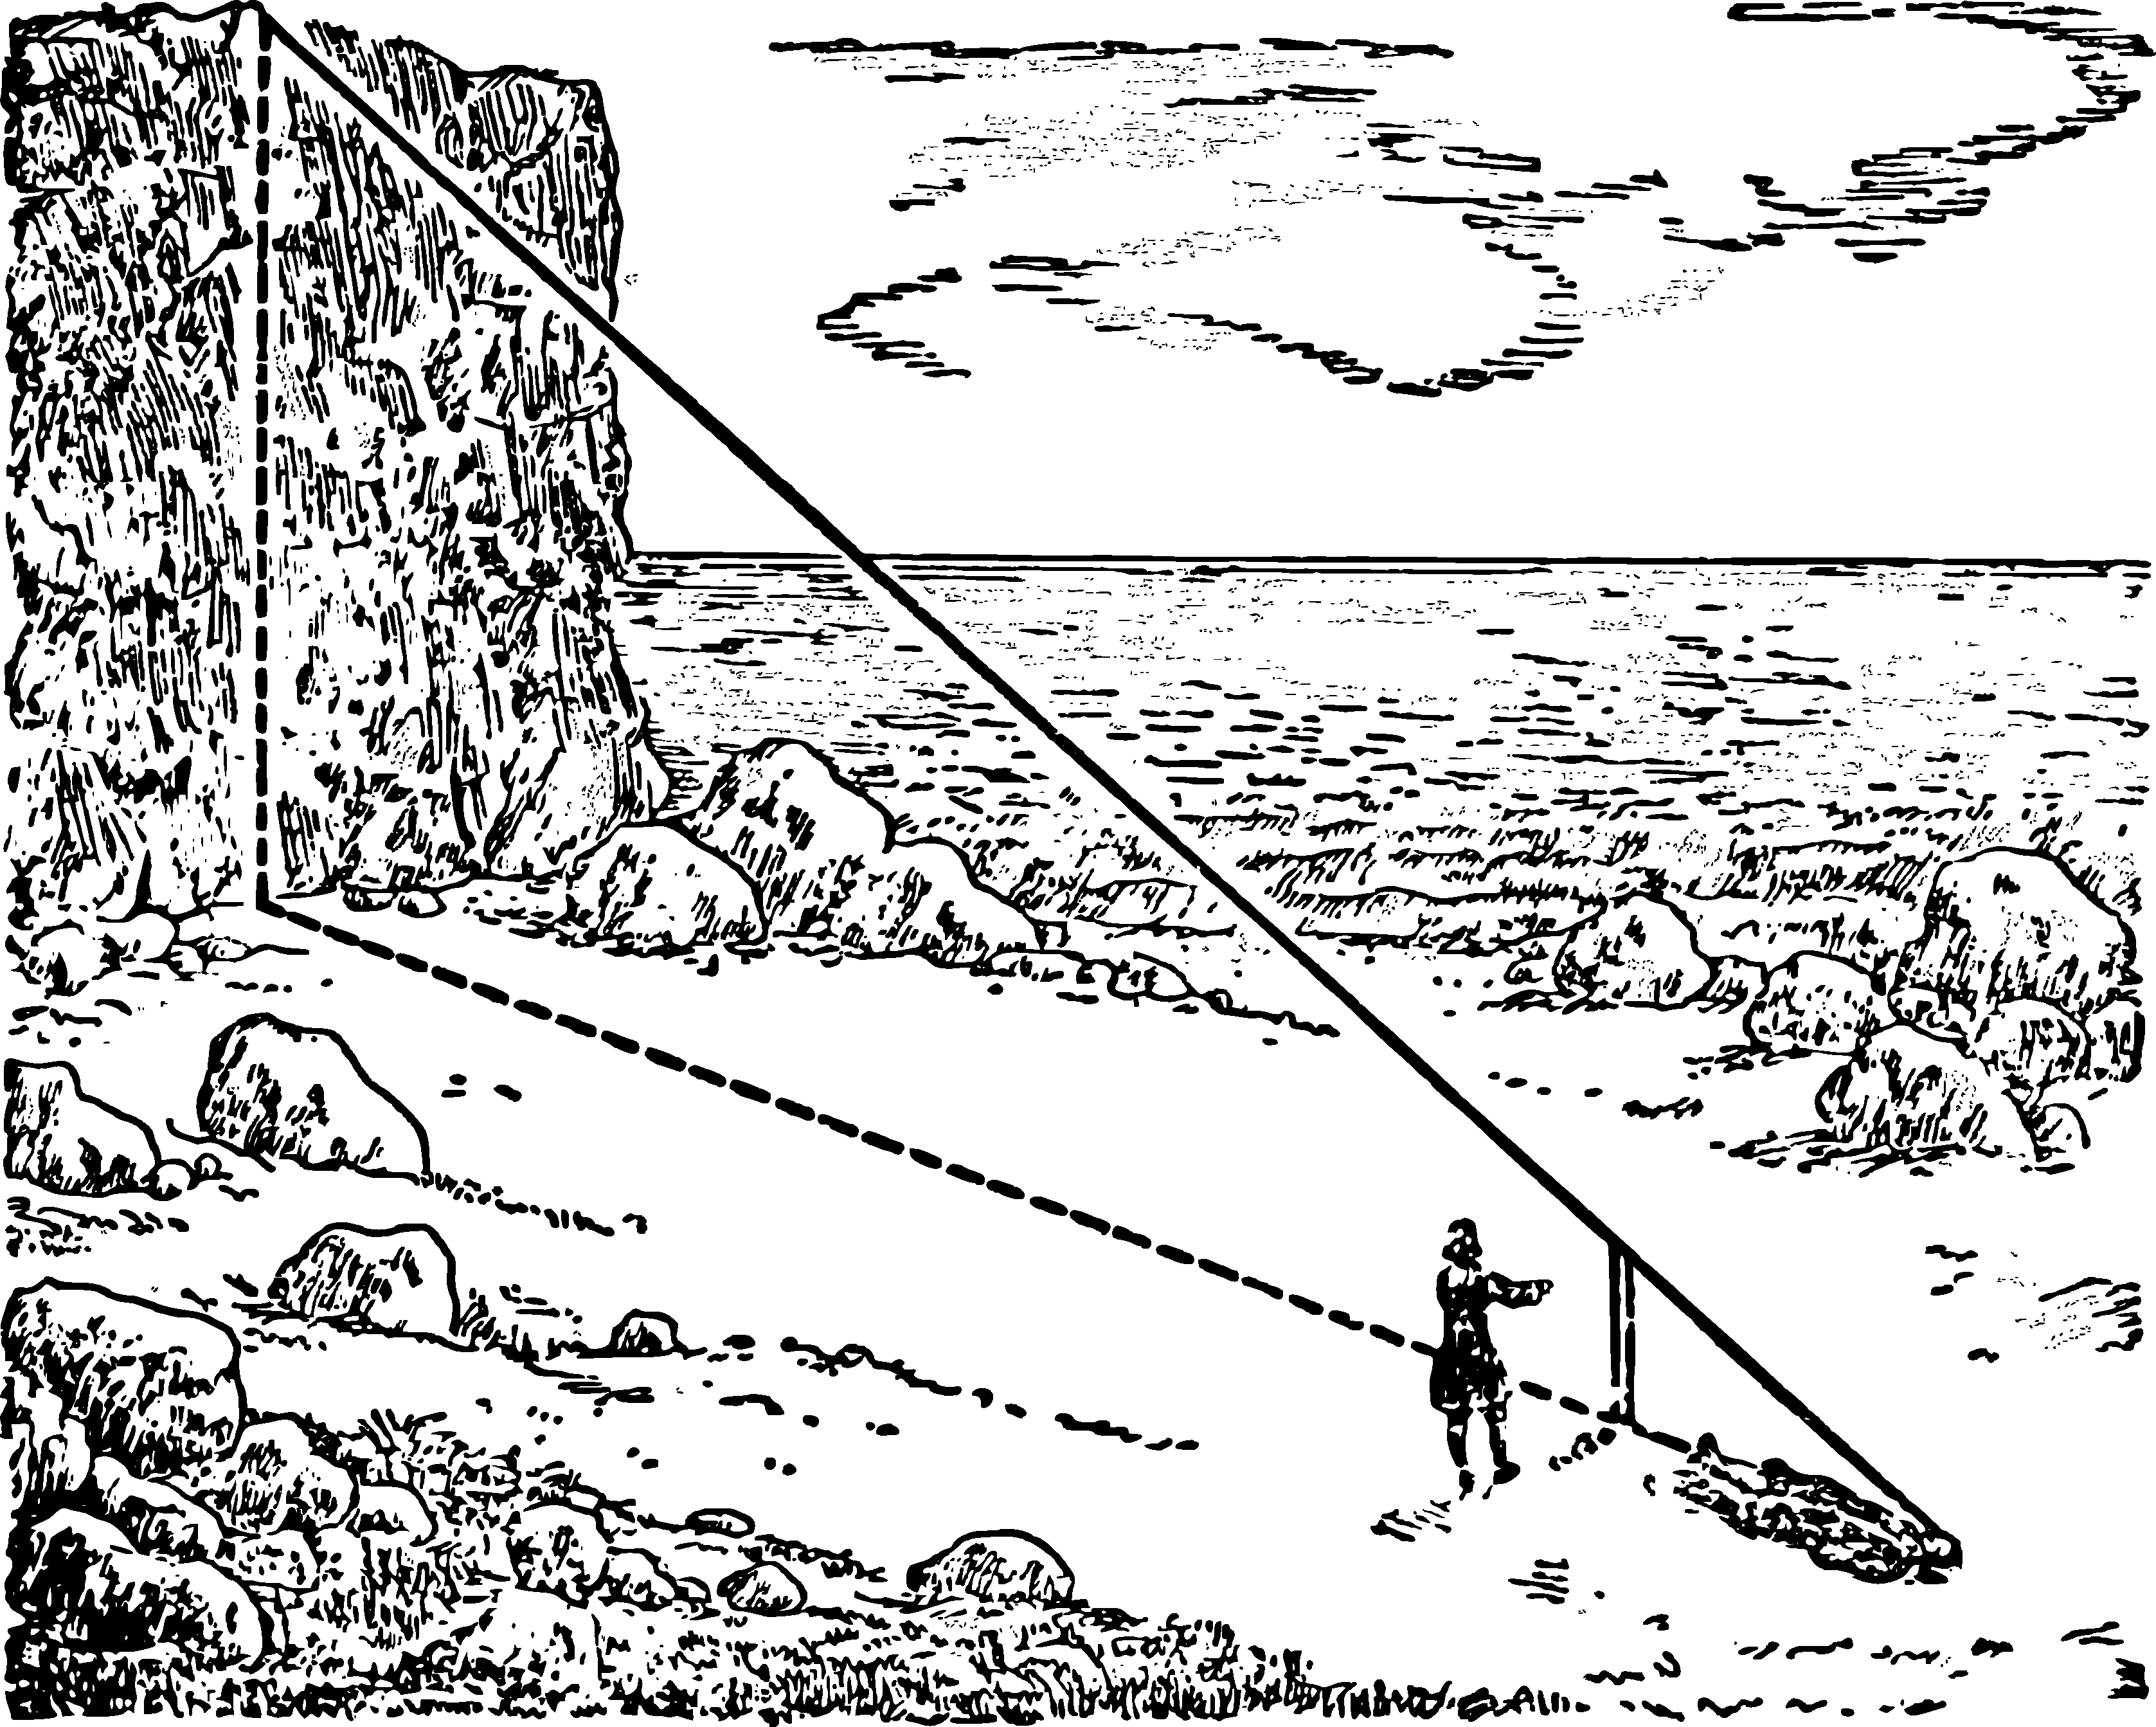
\includegraphics[width=0.9\textwidth]{figures/ch-01/fig-01-07.pdf}
\sidecaption{How the heroes of Jules Verne measured the height of the cliff.\label{fig-01-07}}
\end{figure}

Then he moved away from the pole to a distance where, lying on the sand, one could see both the end of the pole and the edge of the ridge in a straight line (see \figr{fig-01-07}). He carefully marked this point with a stake.

``Are you familiar with the basics of geometry?'' he asked Herbert as he rose from the ground.

``Yes.''

``Do you remember the properties of similar triangles?''

``Their corresponding sides are proportional.''

``Exactly. So now I'll construct two similar right triangles. In the smaller one, one leg will be the plumb-line pole, and the other will be the distance from the stake to the base of the pole; the hypotenuse will be my line of sight. In the other triangle, the legs will be: the granite wall, the height of which we want to determine, and the distance from the stake to the base of this wall; the hypotenuse will be my line of sight, coinciding with the direction of the hypotenuse of the first triangle.''

``Understood!'' exclaimed the youth. ``The distance from the stake to the pole is related to the distance from the stake to the base of the wall, as the height of the pole is to the height of the wall.''

``Yes. And consequently, if we measure the first two distances, then, knowing the height of the pole, we can calculate the fourth, unknown term of the proportion, i.e., the height of the wall. In this way, we can manage without directly measuring the height.''

Both horizontal distances were measured: the smaller one was 15 feet, the larger one was 500 feet.

At the end of the measurements, the engineer made the following record:
\begin{align*}%
15 : 500 & = 10 : x,\\
500 \times 10 & = 5000,\\
5000 : 15 & = 333.3.
\end{align*}
Thus, the height of the granite wall was 333 feet.


\section{How Sergeant Popov Acted}
\label{sec-1.4}

Some of the methods described for measuring height are inconvenient as they require lying on the ground. This inconvenience can, of course, be avoided.

Here's a story from one of the fronts of the Great Patriotic War. Lieutenant Ivanyuk's unit was ordered to build a bridge across a mountain river. On the opposite bank were entrenched fascists. To scout the location for the bridge, the lieutenant assigned a reconnaissance group led by Senior Sergeant Popov. In the nearest forest, they measured the diameter and height of the most typical trees and counted the number of trees that could be used for construction.

They measured the height of the trees using a pole (stick) as shown in \figr{fig-01-08}.

\begin{figure}[h!]
\centering
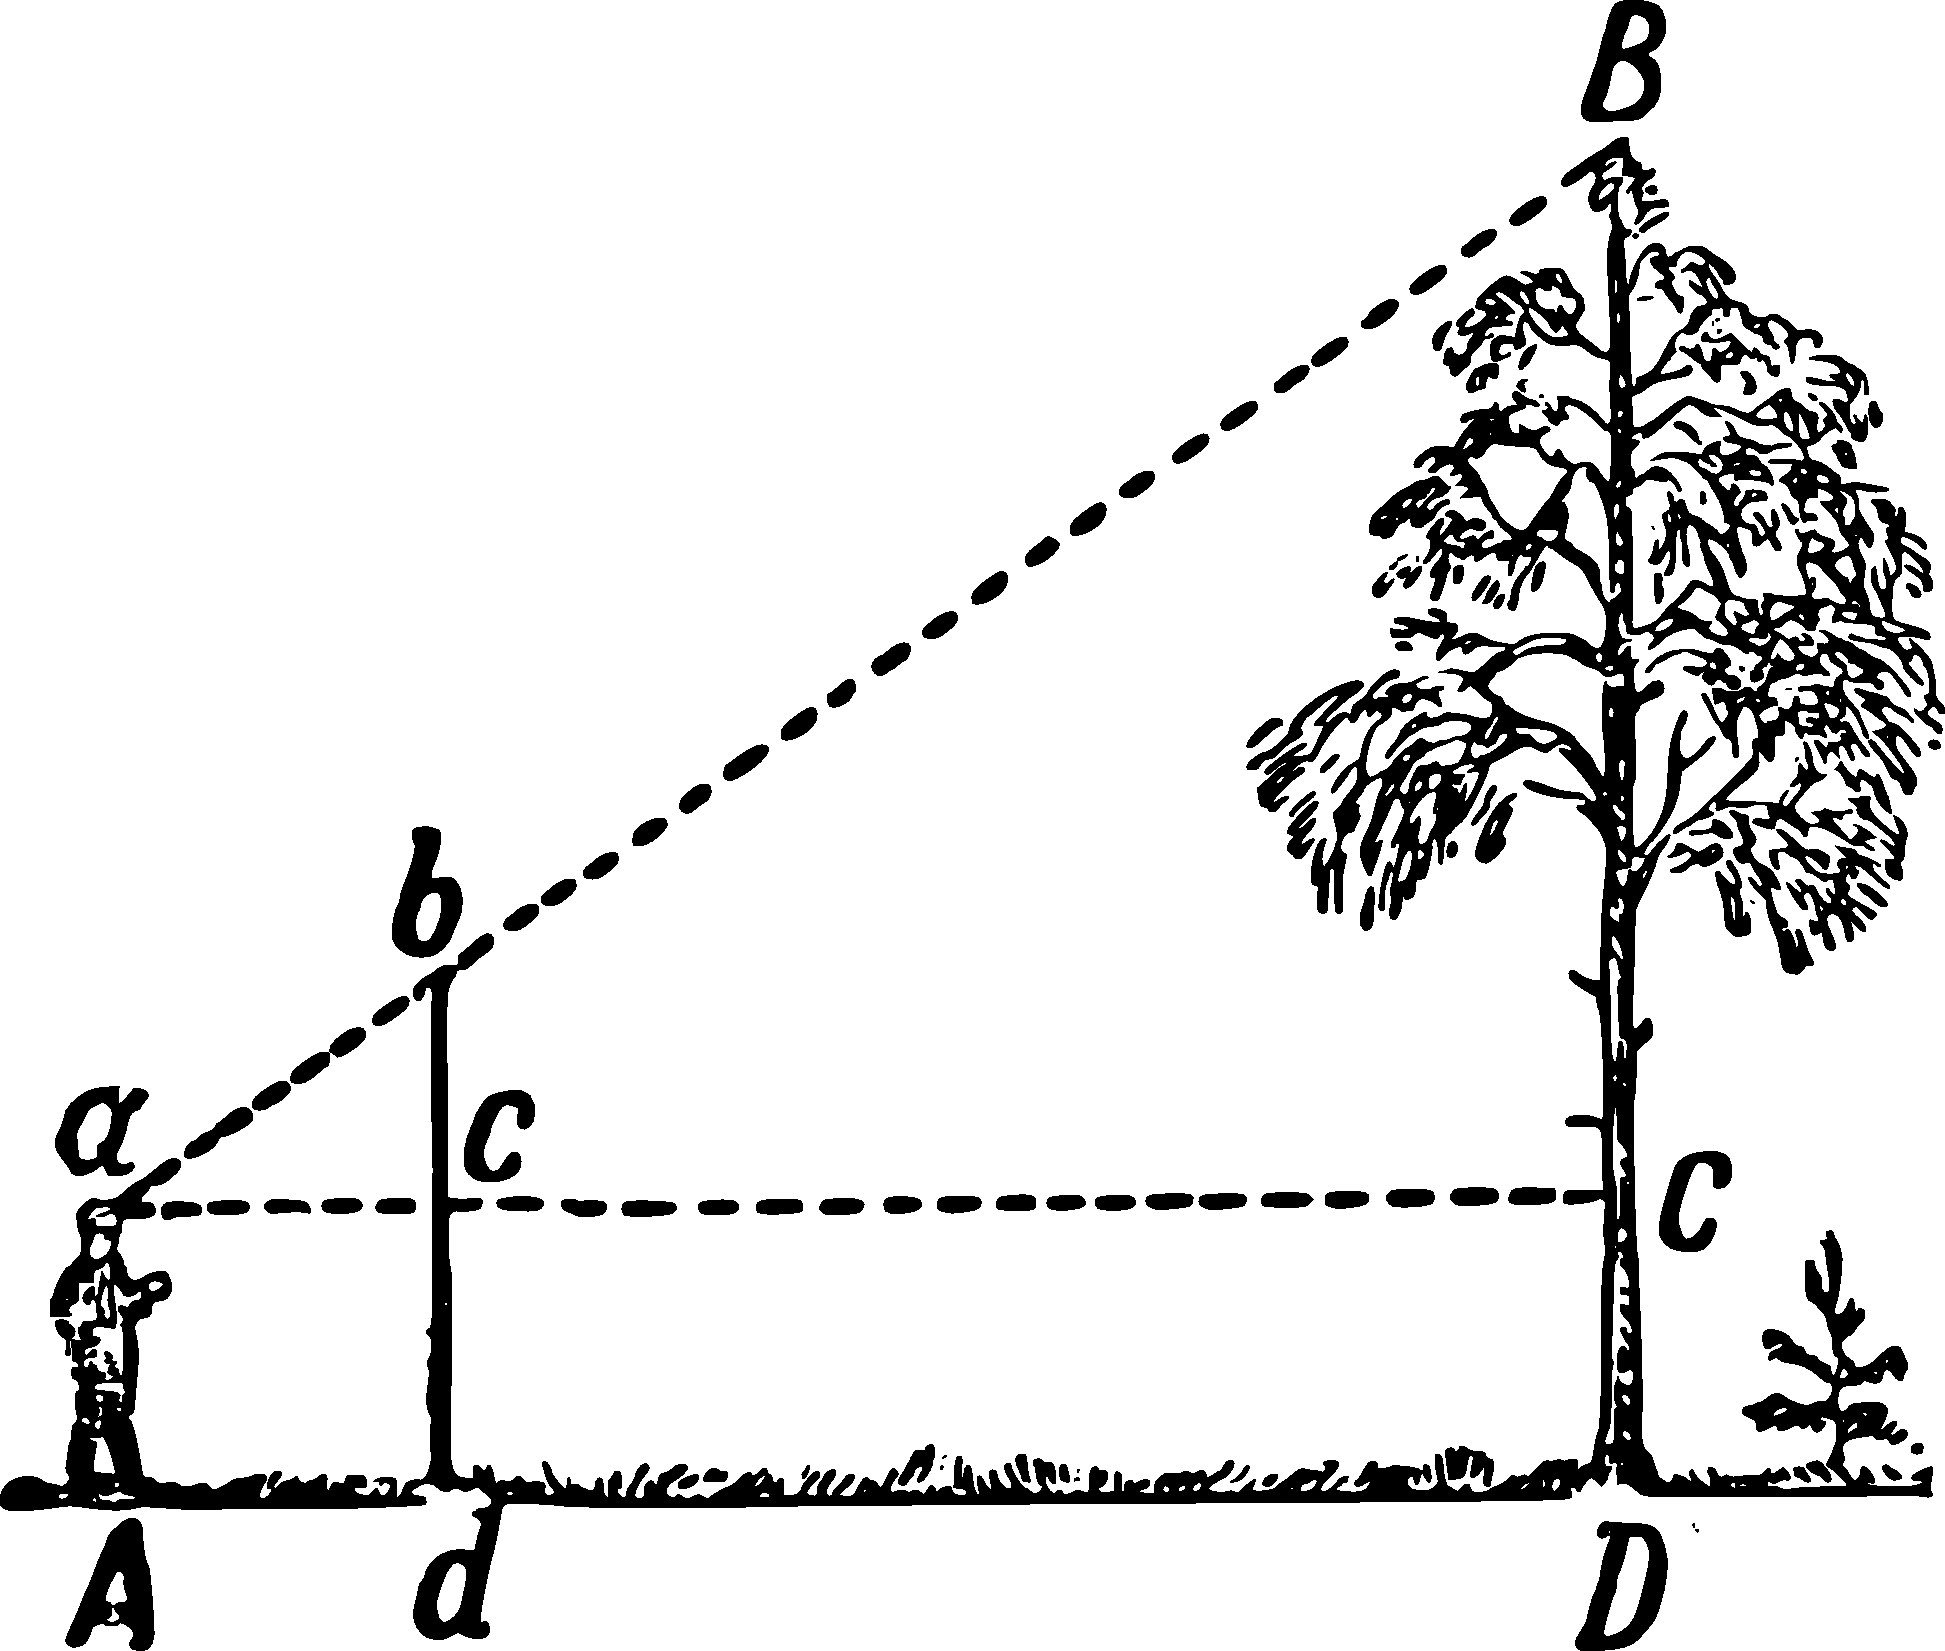
\includegraphics[width=0.6\textwidth]{figures/ch-01/fig-01-08.pdf}
\sidecaption{Measuring the height of the trees with a pole.\label{fig-01-08}}
\end{figure}

This method works as follows: Armed with a pole taller than your own height, drive it into the ground vertically at some distance from the tree being measured (see \figr{fig-01-08}). Step back from the pole along the line $dD$ until you reach point $A$, from where, looking at the top of the tree, you'll see the upper point $B$ of the pole aligned with it. Then, without changing the position of your head, look along the horizontal line $aC$, noting the point $C$ where your line of sight intersects the pole and the tree trunk. Ask your assistant to mark these points, and the observation is complete. Then, based on the similarity of triangles $abc$ and $aBC$, calculate $BC$ from the proportion 
\begin{equation*}%
\frac{BC}{bc} = \frac{aC}{ac},
\end{equation*}
and thus
\begin{equation*}%
BC = bc \cdot \frac{aC}{ac}
\end{equation*}
The distances $bc$, $aC$, and $ac$ can be easily measured directly. To obtain the actual height of the tree, add the distance $BC$ to the distance $CD$, which is also measured directly.

To determine the number of trees, the senior sergeant ordered the soldiers to measure the area of the forest. Then he counted the number of trees in a small area measuring 50 by 50 meters and multiplied accordingly.

Based on all the data collected by the scouts, the unit commander determined where and what kind of bridge needed to be built. The bridge was completed on time, and the combat mission was successfully accomplished!\sidenote{The episodes of the Great Patriotic War described here and further are narrated by A. Demidov in the journal \emph{Military Knowledge} No. 8, 1949, in the article \emph{River Reconnaissance.}\label{ref-21}}

\clearpage

\section{Using a Notebook}
\label{sec-1.5}

As a device for an approximate estimate of the inaccessible height, you can also use your pocket back book, if it is equipped with a pencil stuck in a cover or a loop with a book. It will help you to build in space those two similar triangles, from which the desired height is obtained. The book should be held near the eyes as shown in the simplified \figr{fig-01-09}. It should be in the vertical book so that, looking from the point $a$, you can see the top of the tree $B$ covered with the tip of the pencil $b$. Then, due to the similarity of the triangles $abc$ and $aBC$, the height of the $BC$ will be determined from the proportion
\begin{equation*}%
\frac{BC}{bc} = \frac{aC}{ac}.
\end{equation*}
The distances of $bc$, $ac$ and $aC$ are measured directly. To the resulting value of the $BC$, add the length of $CD$, which is, on level ground, the height of the eyes above the ground


\begin{figure}[h!]
\centering
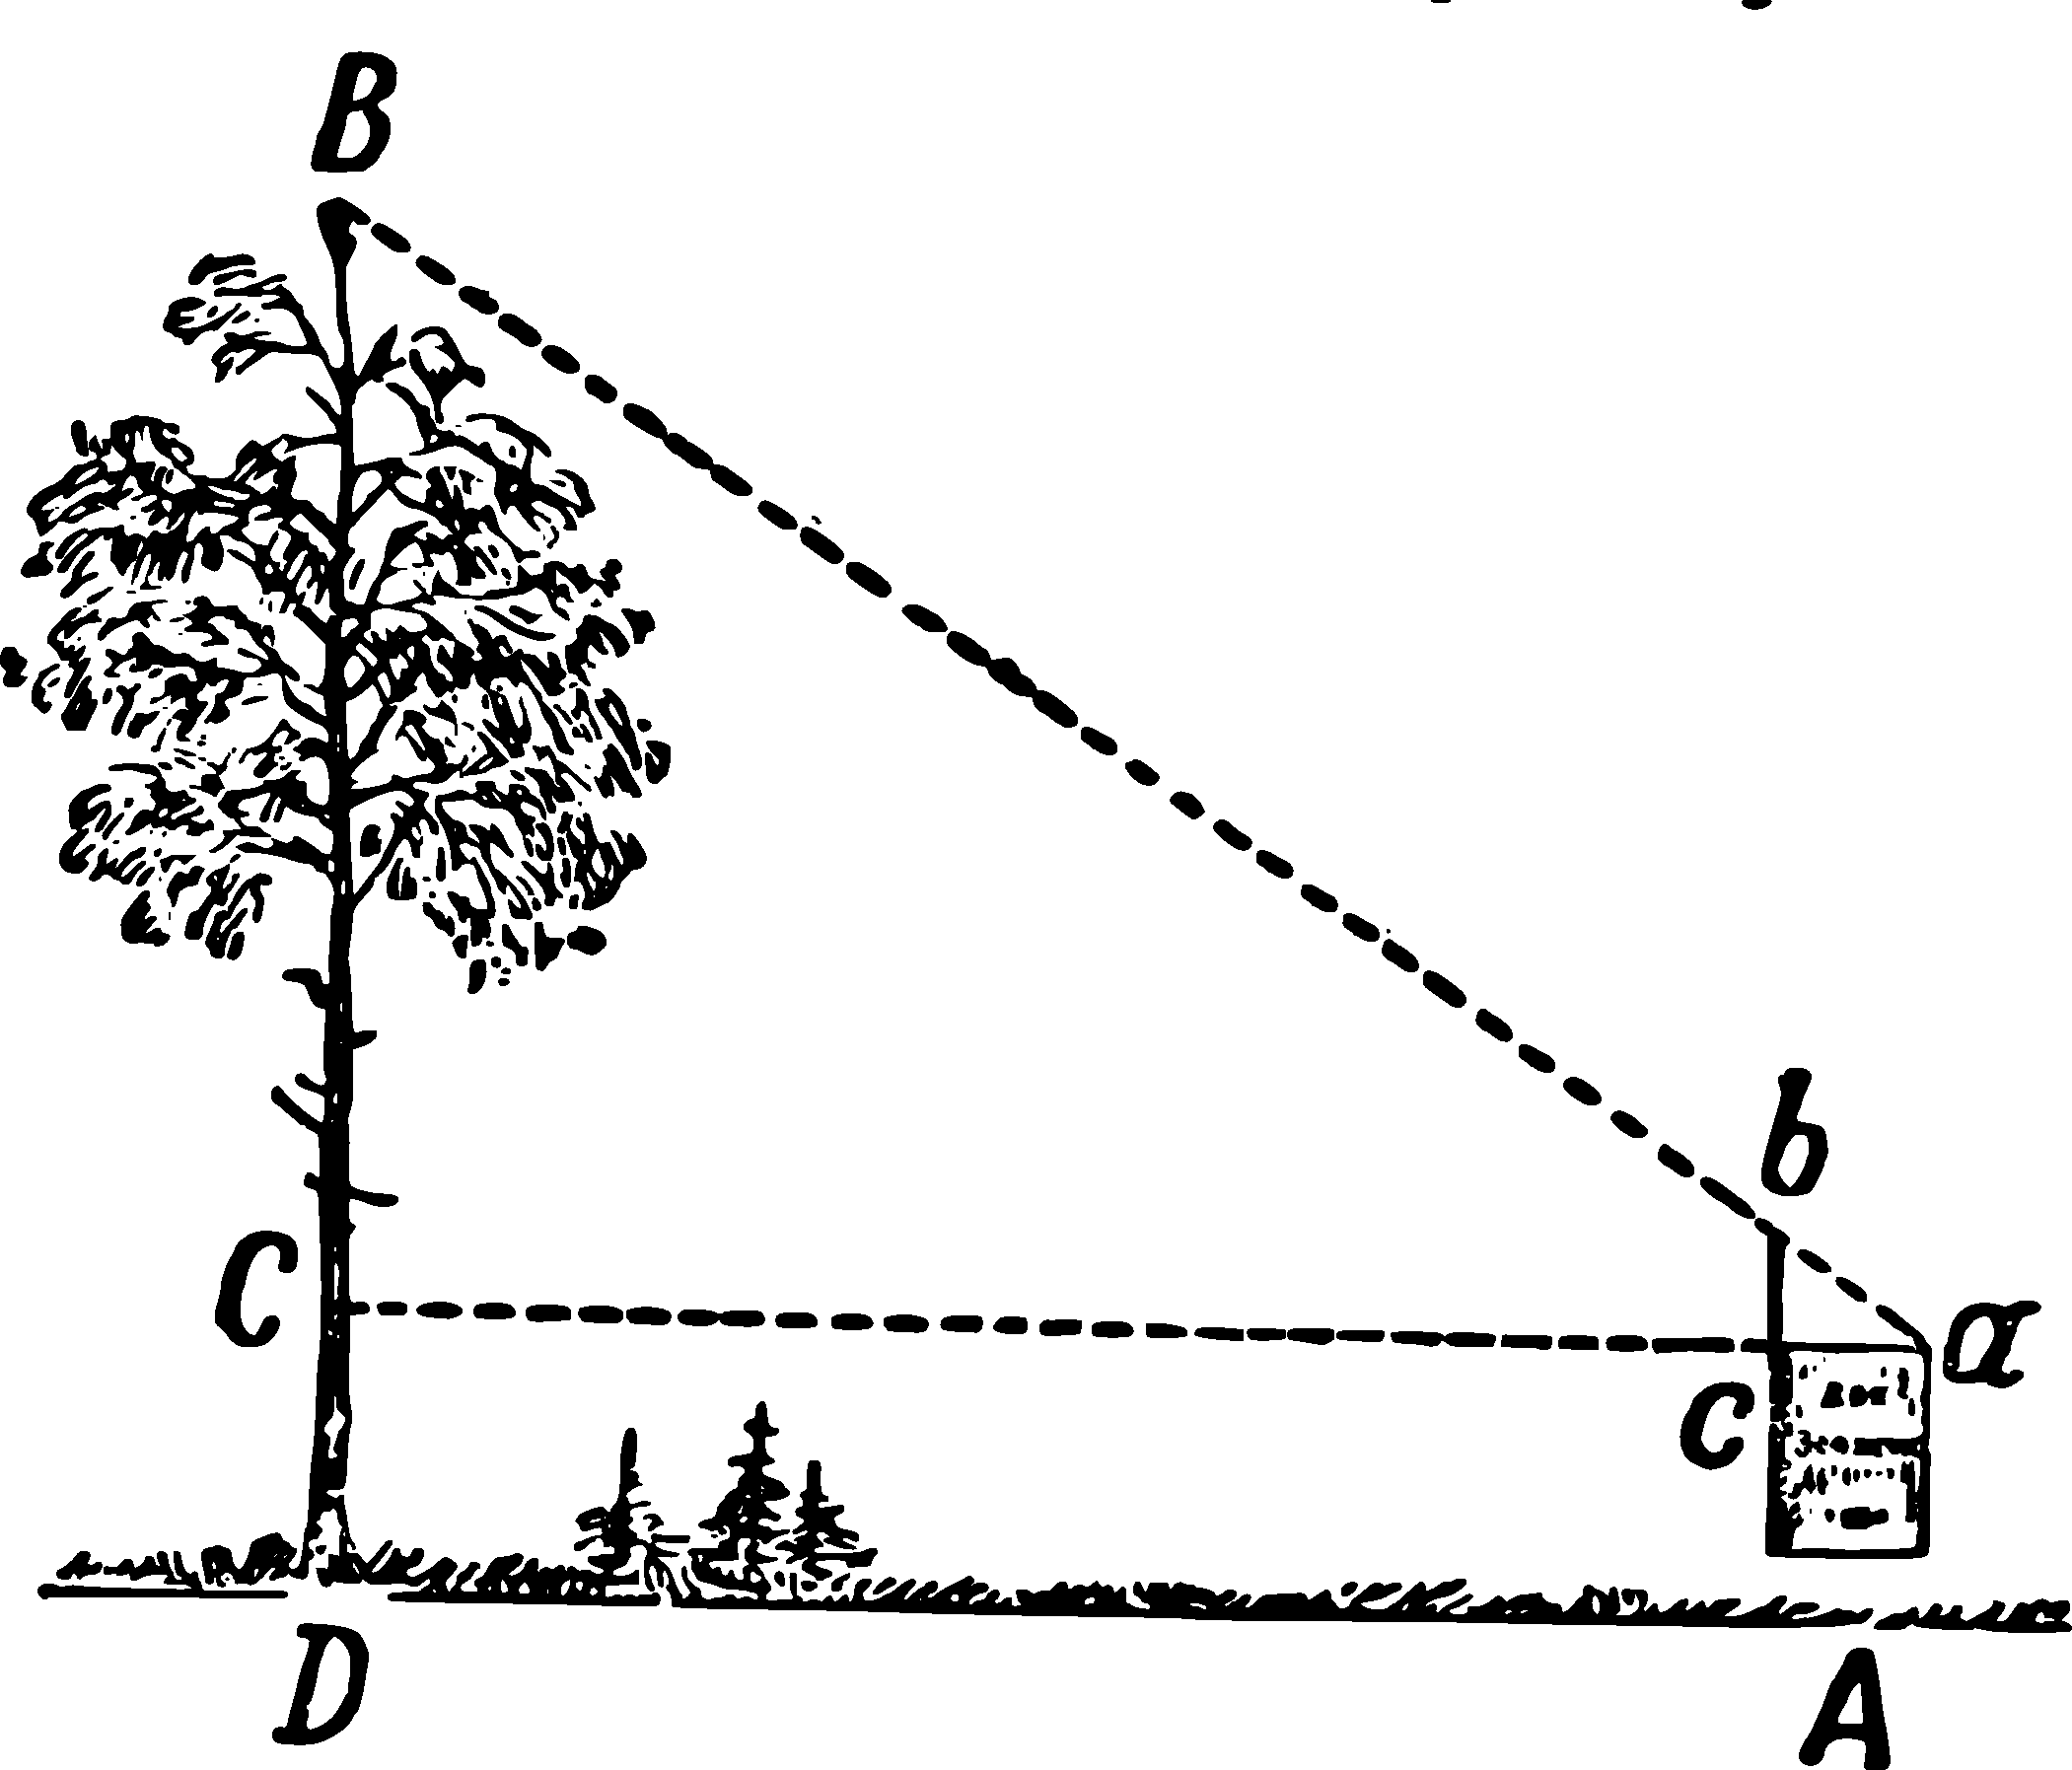
\includegraphics[width=0.6\textwidth]{figures/ch-01/fig-01-09.pdf}
\sidecaption{Height measurement using a notebook.\label{fig-01-09}}
\end{figure}

Since the width of the $ac$ book is unchanged, if you always stand at the same distance from the measured tree (for example, \SI{10}{\meter}), the height of the tree will depend only on the extended part of the pencil. Therefore, you can calculate in advance what height corresponds to a particular extension, and put these numbers on the pencil. Your notebook will then turn into a simplified altimeter, since you can use it to determine heights immediately, without calculations.





\section{Without Approaching The Tree}
\label{sec-1.6}

Sometimes it may be inconvenient to get close to the base of the tree being measured. Can its height still be determined in such a case?

Absolutely. For this purpose, a clever device has been devised, which, like the previous ones, is easy to make by yourself. Two planks, $ab$ and $cd$ (top of \figr{fig-01-10}), are fastened together at right angles so that $ab$ equals $bc$, and $bd$ equals half of $ab$. That's the whole device. 

To measure height with it, hold it in your hands, directing plank CD vertically (for which it has a plumb line with a weight), and stand precisely in two places: first (\figr{fig-01-10}) at point $A$, where the device is positioned with end $c$ up, and then at point $A'$, a bit farther away, where the device is held with end $d$ up. Point $A$ is chosen so that, looking from $a$ to the end of $a$, it is seen on the same line as the top of the tree. Point $A'$ is found so that, looking from $a'$ to point $d'$, it is seen coinciding with $B$. 

The discovery of these two points $A$ and $A'$\sidenote{These points must necessarily lie in a straight line with the base of the tree.} constitutes all the measurement because the desired part of the tree's height, $BC$, is equal to the distance $DA'$. The equality follows easily from the fact that $aC = BC$ and $a'C = 2BC$; thus,
\begin{equation*}%
a'C - aC = BC.
\end{equation*}


\begin{figure}[h!]
\centering
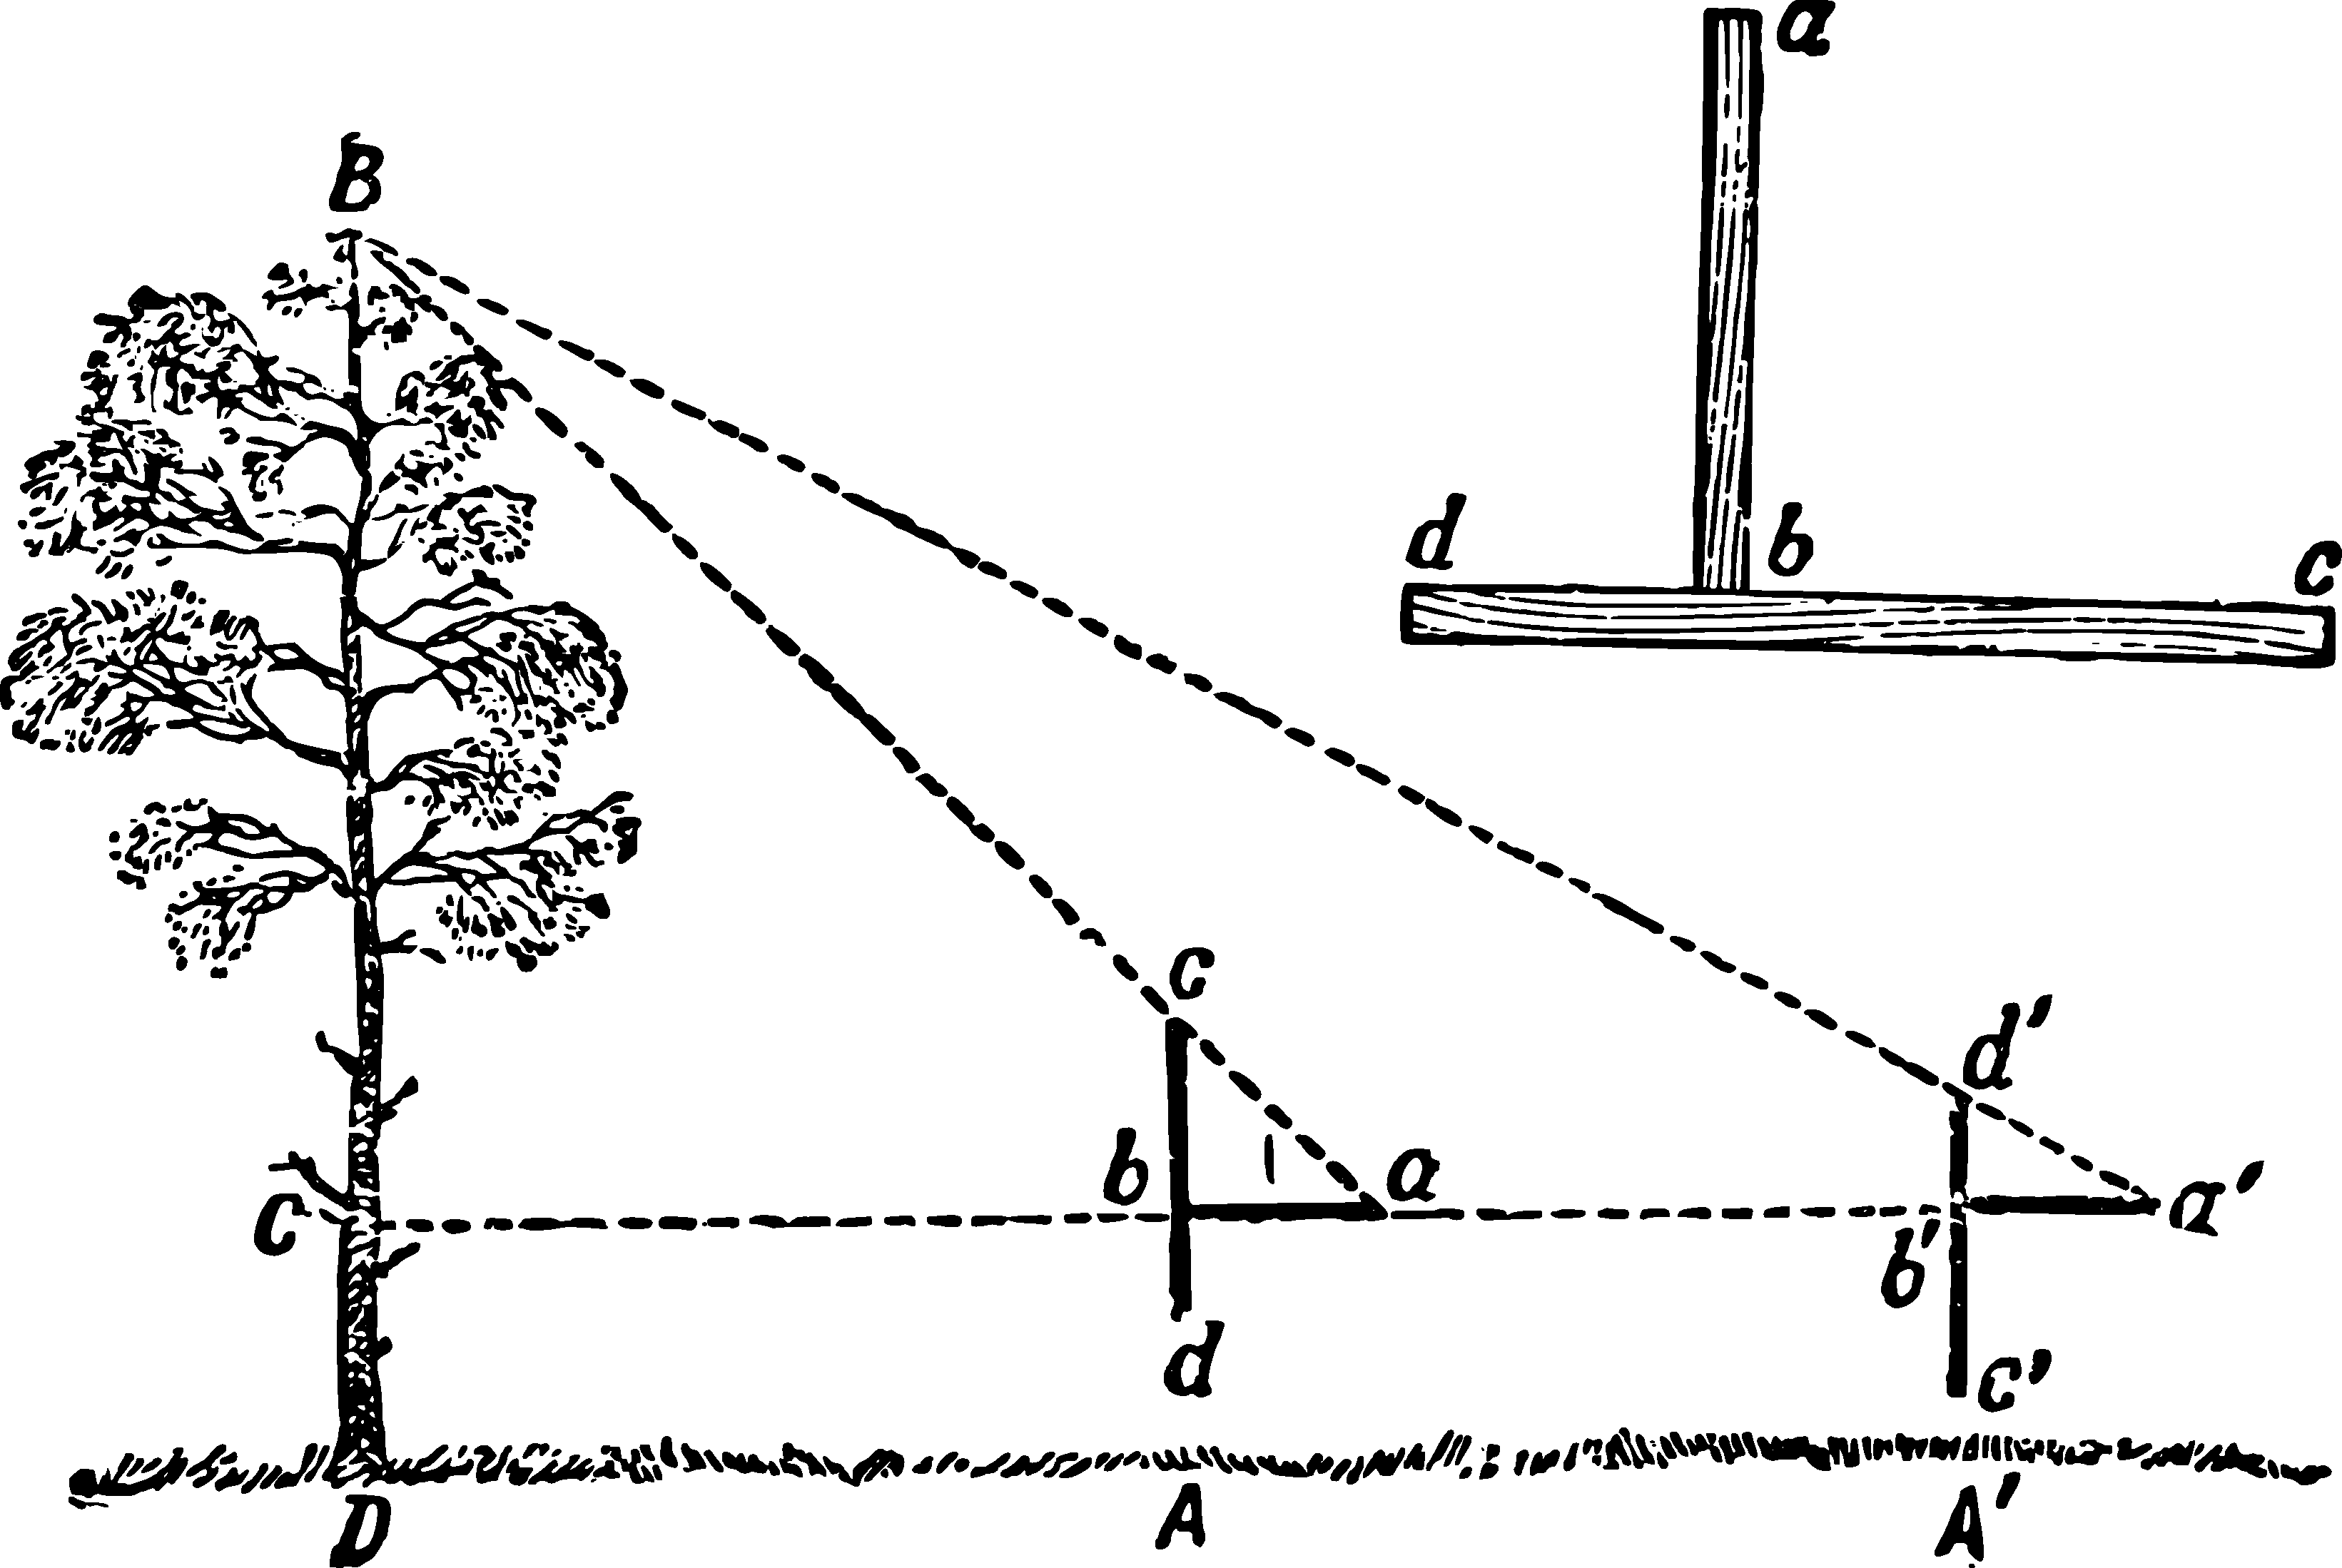
\includegraphics[width=0.8\textwidth]{figures/ch-01/fig-01-10.pdf}
\sidecaption{The use of a simple altimeter consisting of two planks.\label{fig-01-10}}
\end{figure}




You can see that using this simple device, we measure the tree's height without approaching closer than its height. It goes without saying that if it's possible to approach the trunk, it's sufficient to find just one of the points -- $A$ or $A'$ -- to determine its height.

Instead of two planks, you can use four pins, arranging them on a board properly; in this form, the ``device'' is even simpler.

%\clearpage

\section{Forest Rangers' Altimeter}
\label{sec-1.7}

It's time to explain how the ``real'' altimeters, used in practise by forest workers, are constructed. I'll describe one of these altimeters, slightly modifying it so that the device can be easily crafted at home. 

\begin{figure}[h!]
\centering
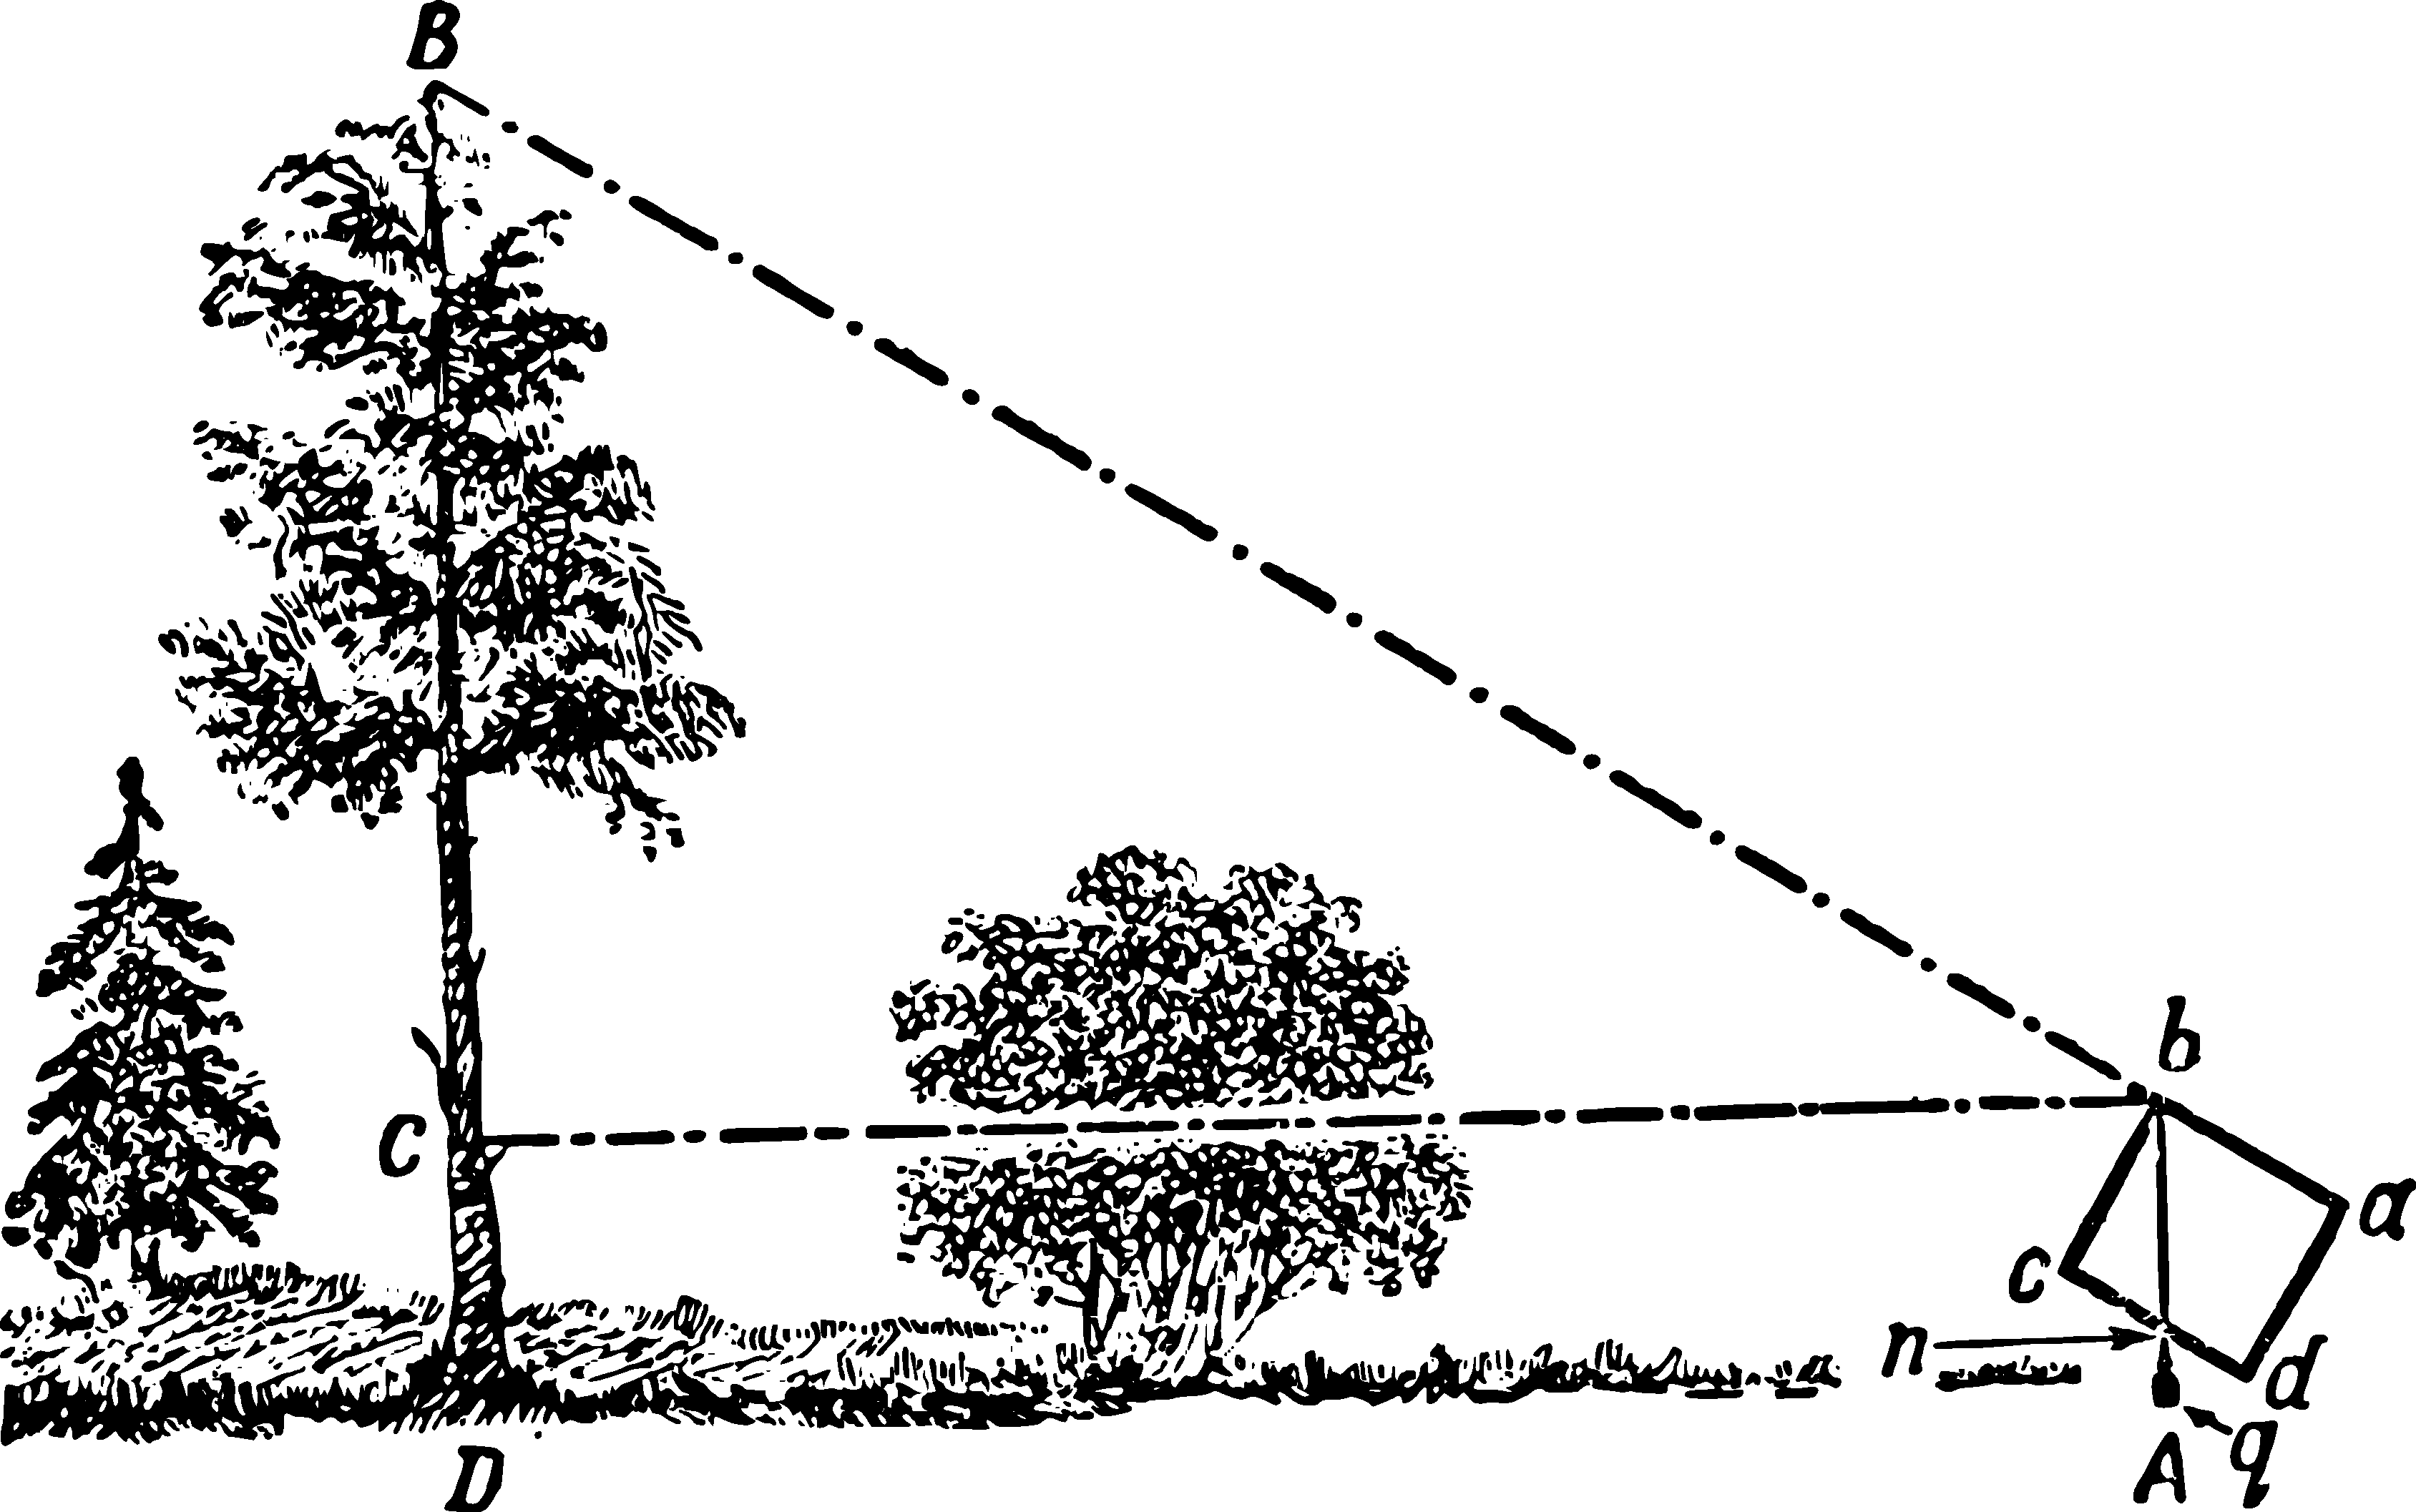
\includegraphics[width=\textwidth]{figures/ch-01/fig-01-11.pdf}
\sidecaption{The scheme of using the altimeter of foresters.\label{fig-01-11}}
\end{figure}


The essence of the device is visible in \figr{fig-01-11}. A cardboard or wooden rectangle, $abcd$, is held in the hand so that, looking along edge $ab$, the tip $B$ of the tree is in line with it. A weight, $q$, is suspended from point $b$ on a thread. We note the point $n$ where the thread intersects line $dc$. Triangles $bBC$ and $bnc$ are similar because they are both rectangular and have equal acute angles $bBC$ and $bnc$ (with corresponding parallel sides). Therefore, we can write the proportion:
\begin{align*}%
\frac{BC}{nc} & = \frac{bC}{bc}; \,\, \text{hence} \\
BC & = bC \cdot \frac{nc}{bc}.
\end{align*}
Since $bC$, $nc$, and $bc$ can be measured directly, it is easy to obtain the desired height of the tree by adding the length of the lower part $CD$ to the trunk (the height of the device above the ground). 

A few details remain to be added. If the edge of the board $bc$ is made, for example, exactly \SI{10}{\centi\meter}, and centimeter divisions are marked on edge $dc$, then the ratio $nc/bc$ will always be expressed as a decimal fraction, directly indicating what fraction of the distance $bC$ represents the height of the tree $BC$. For example, let's say the thread stops against the 7th division mark (i.e., $nc = \SI{7}{\centi\meter}$); this means that the height of the tree above eye level is 0.7 times the observer's distance from the trunk.

\begin{figure}[h!]
\centering
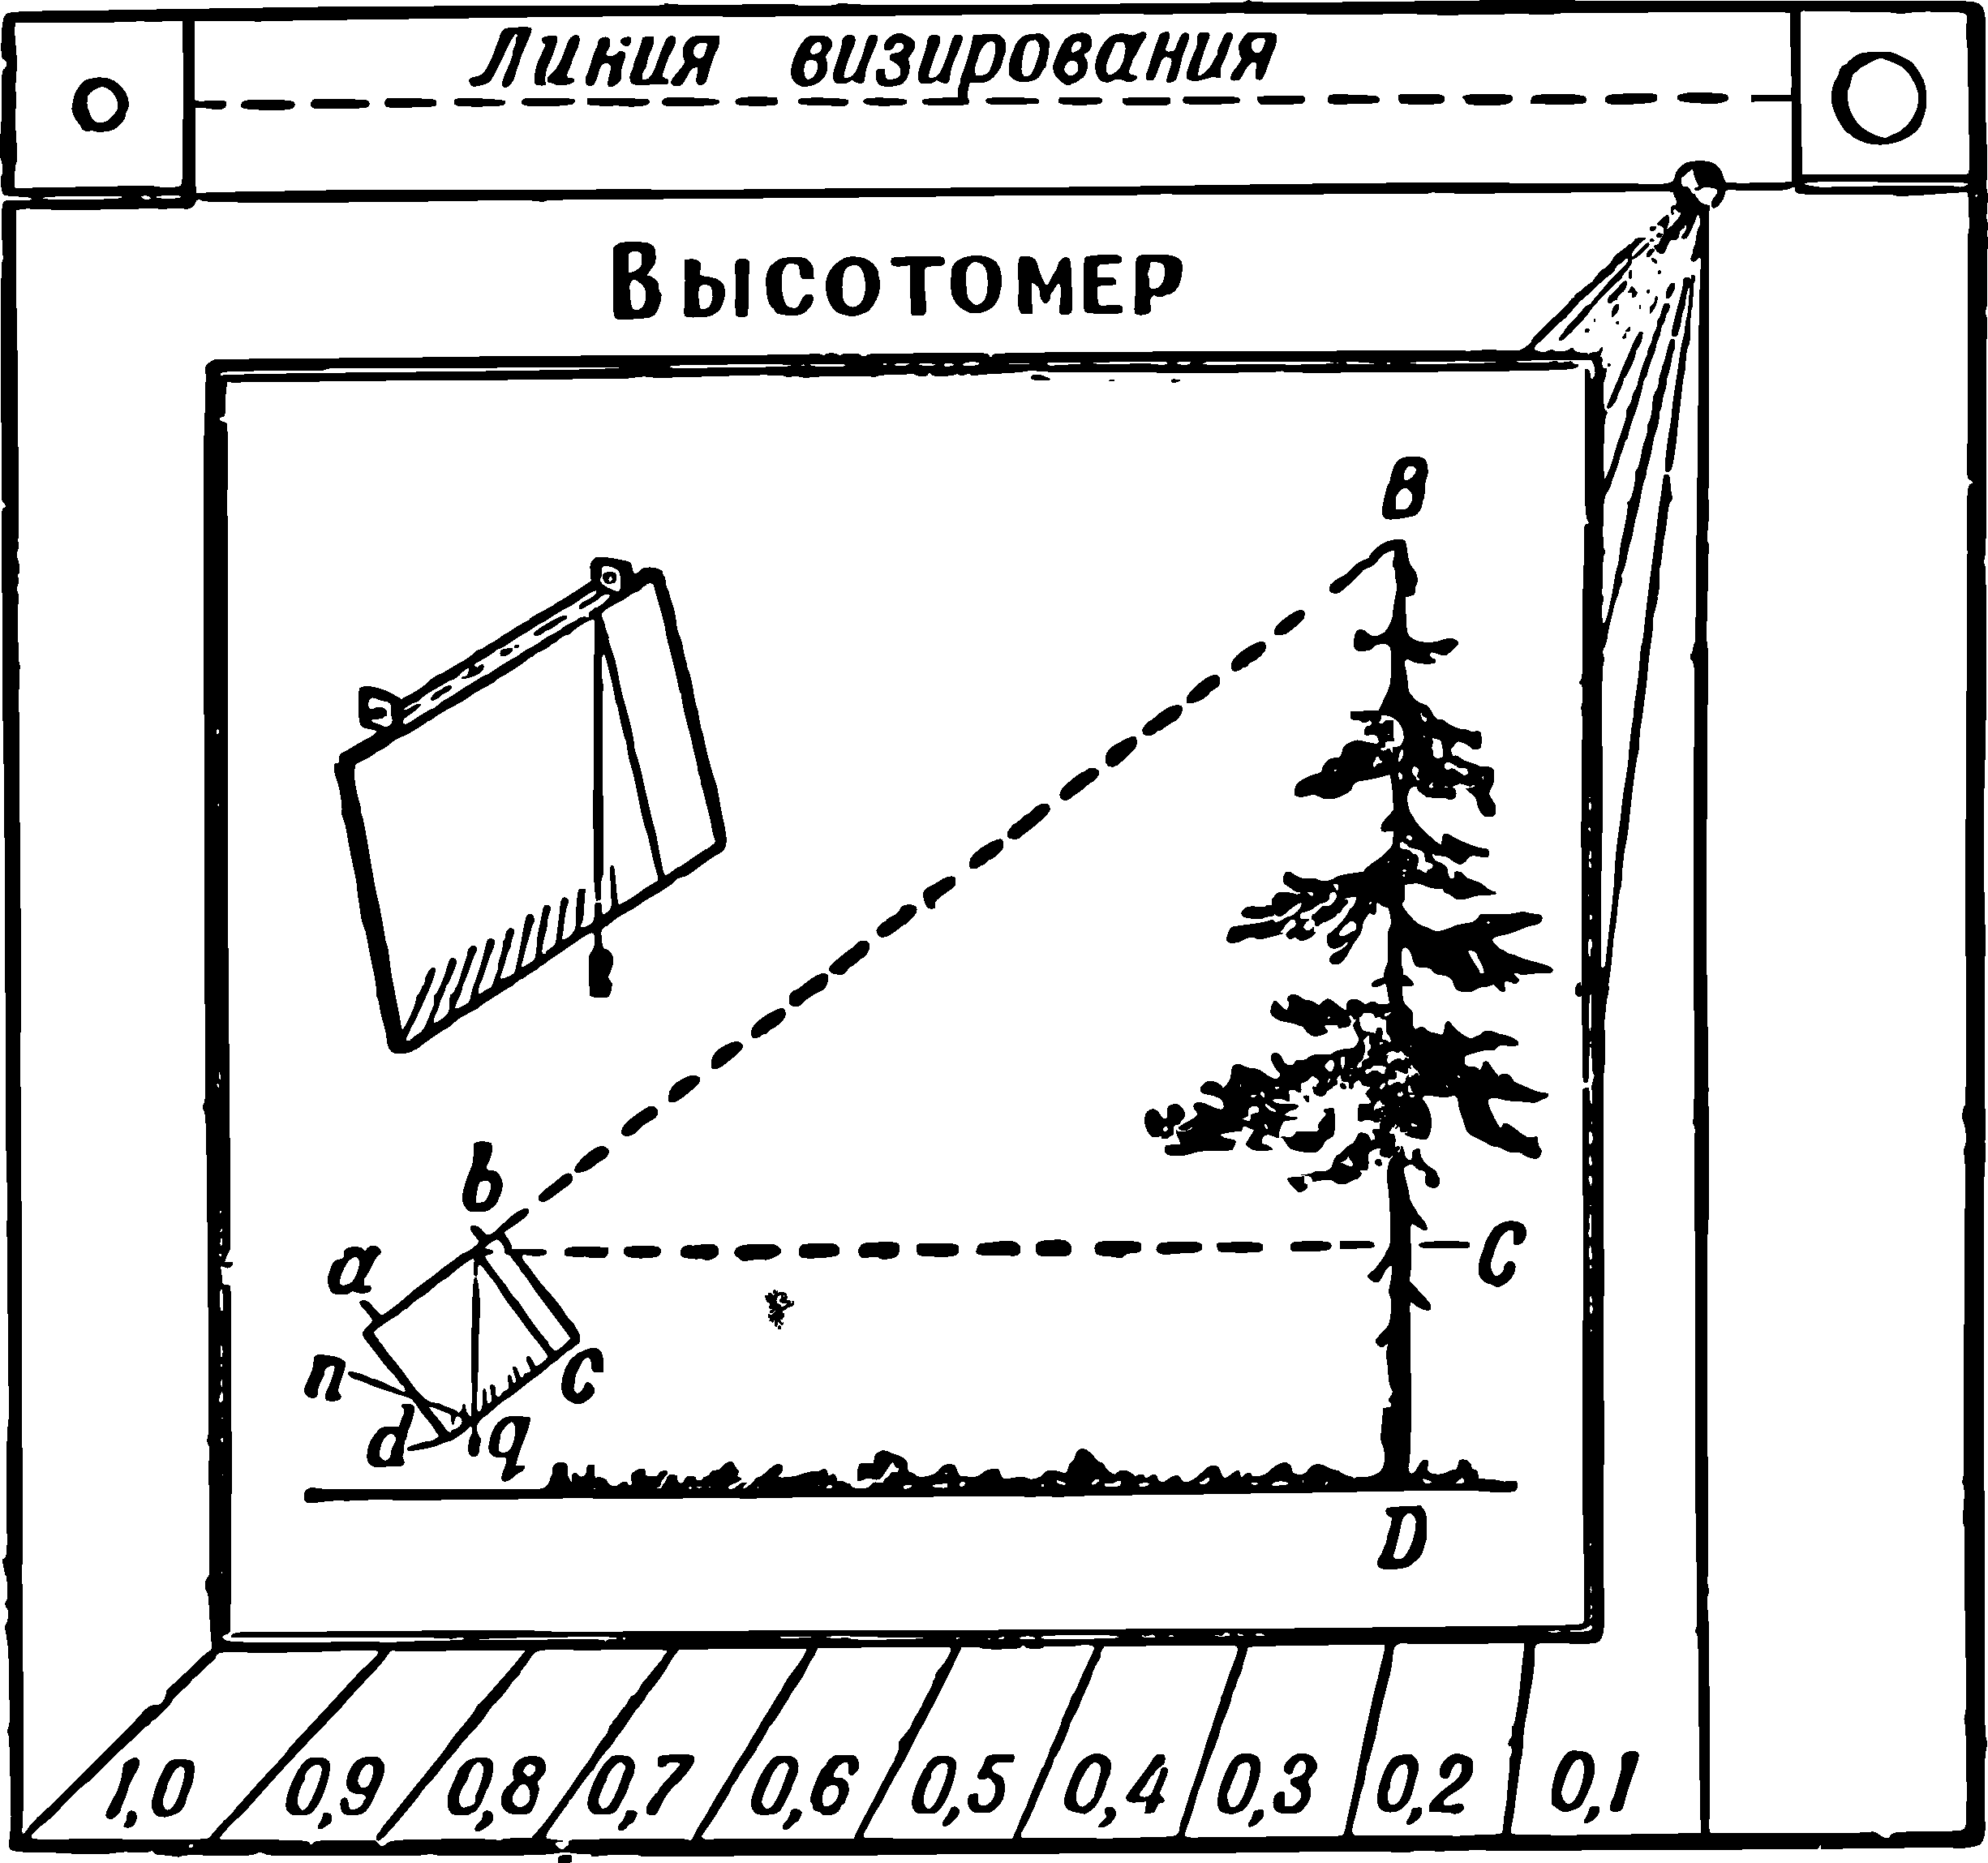
\includegraphics[width=0.7\textwidth]{figures/ch-01/fig-01-12.pdf}
\sidecaption{The forest rangers' altimeter.\label{fig-01-12}}
\end{figure}

The second improvement relates to the method of observation: to make it convenient to look along line $ab$, you can fold down two squares with holes drilled in them at the upper corners of the cardboard rectangle: one smaller one for the eye and one larger one for sighting the tree top (see \figr{fig-01-11}). Further enhancement is represented by the device shown almost to scale in \figr{fig-01-12}. It is easy and quick to make it in this form; no special skill is required. Occupying little space in the pocket, it will provide you with the ability to quickly determine the heights of encountered objects during excursions—trees, poles, buildings, and so on. (This tool is part of the \emph{Geometry in the Open Air} kit developed by the author of this book.)

%\clearpage


\ques Is it possible to use the altimeter described now to measure trees that cannot be approached closely? If possible, what should be done In such cases?


\ans The device should be aimed at the top of the tree $B$, as shown in \figr{fig-01-13}, from two points, $A$ and $A'$. 

\begin{figure}[h!]
\centering
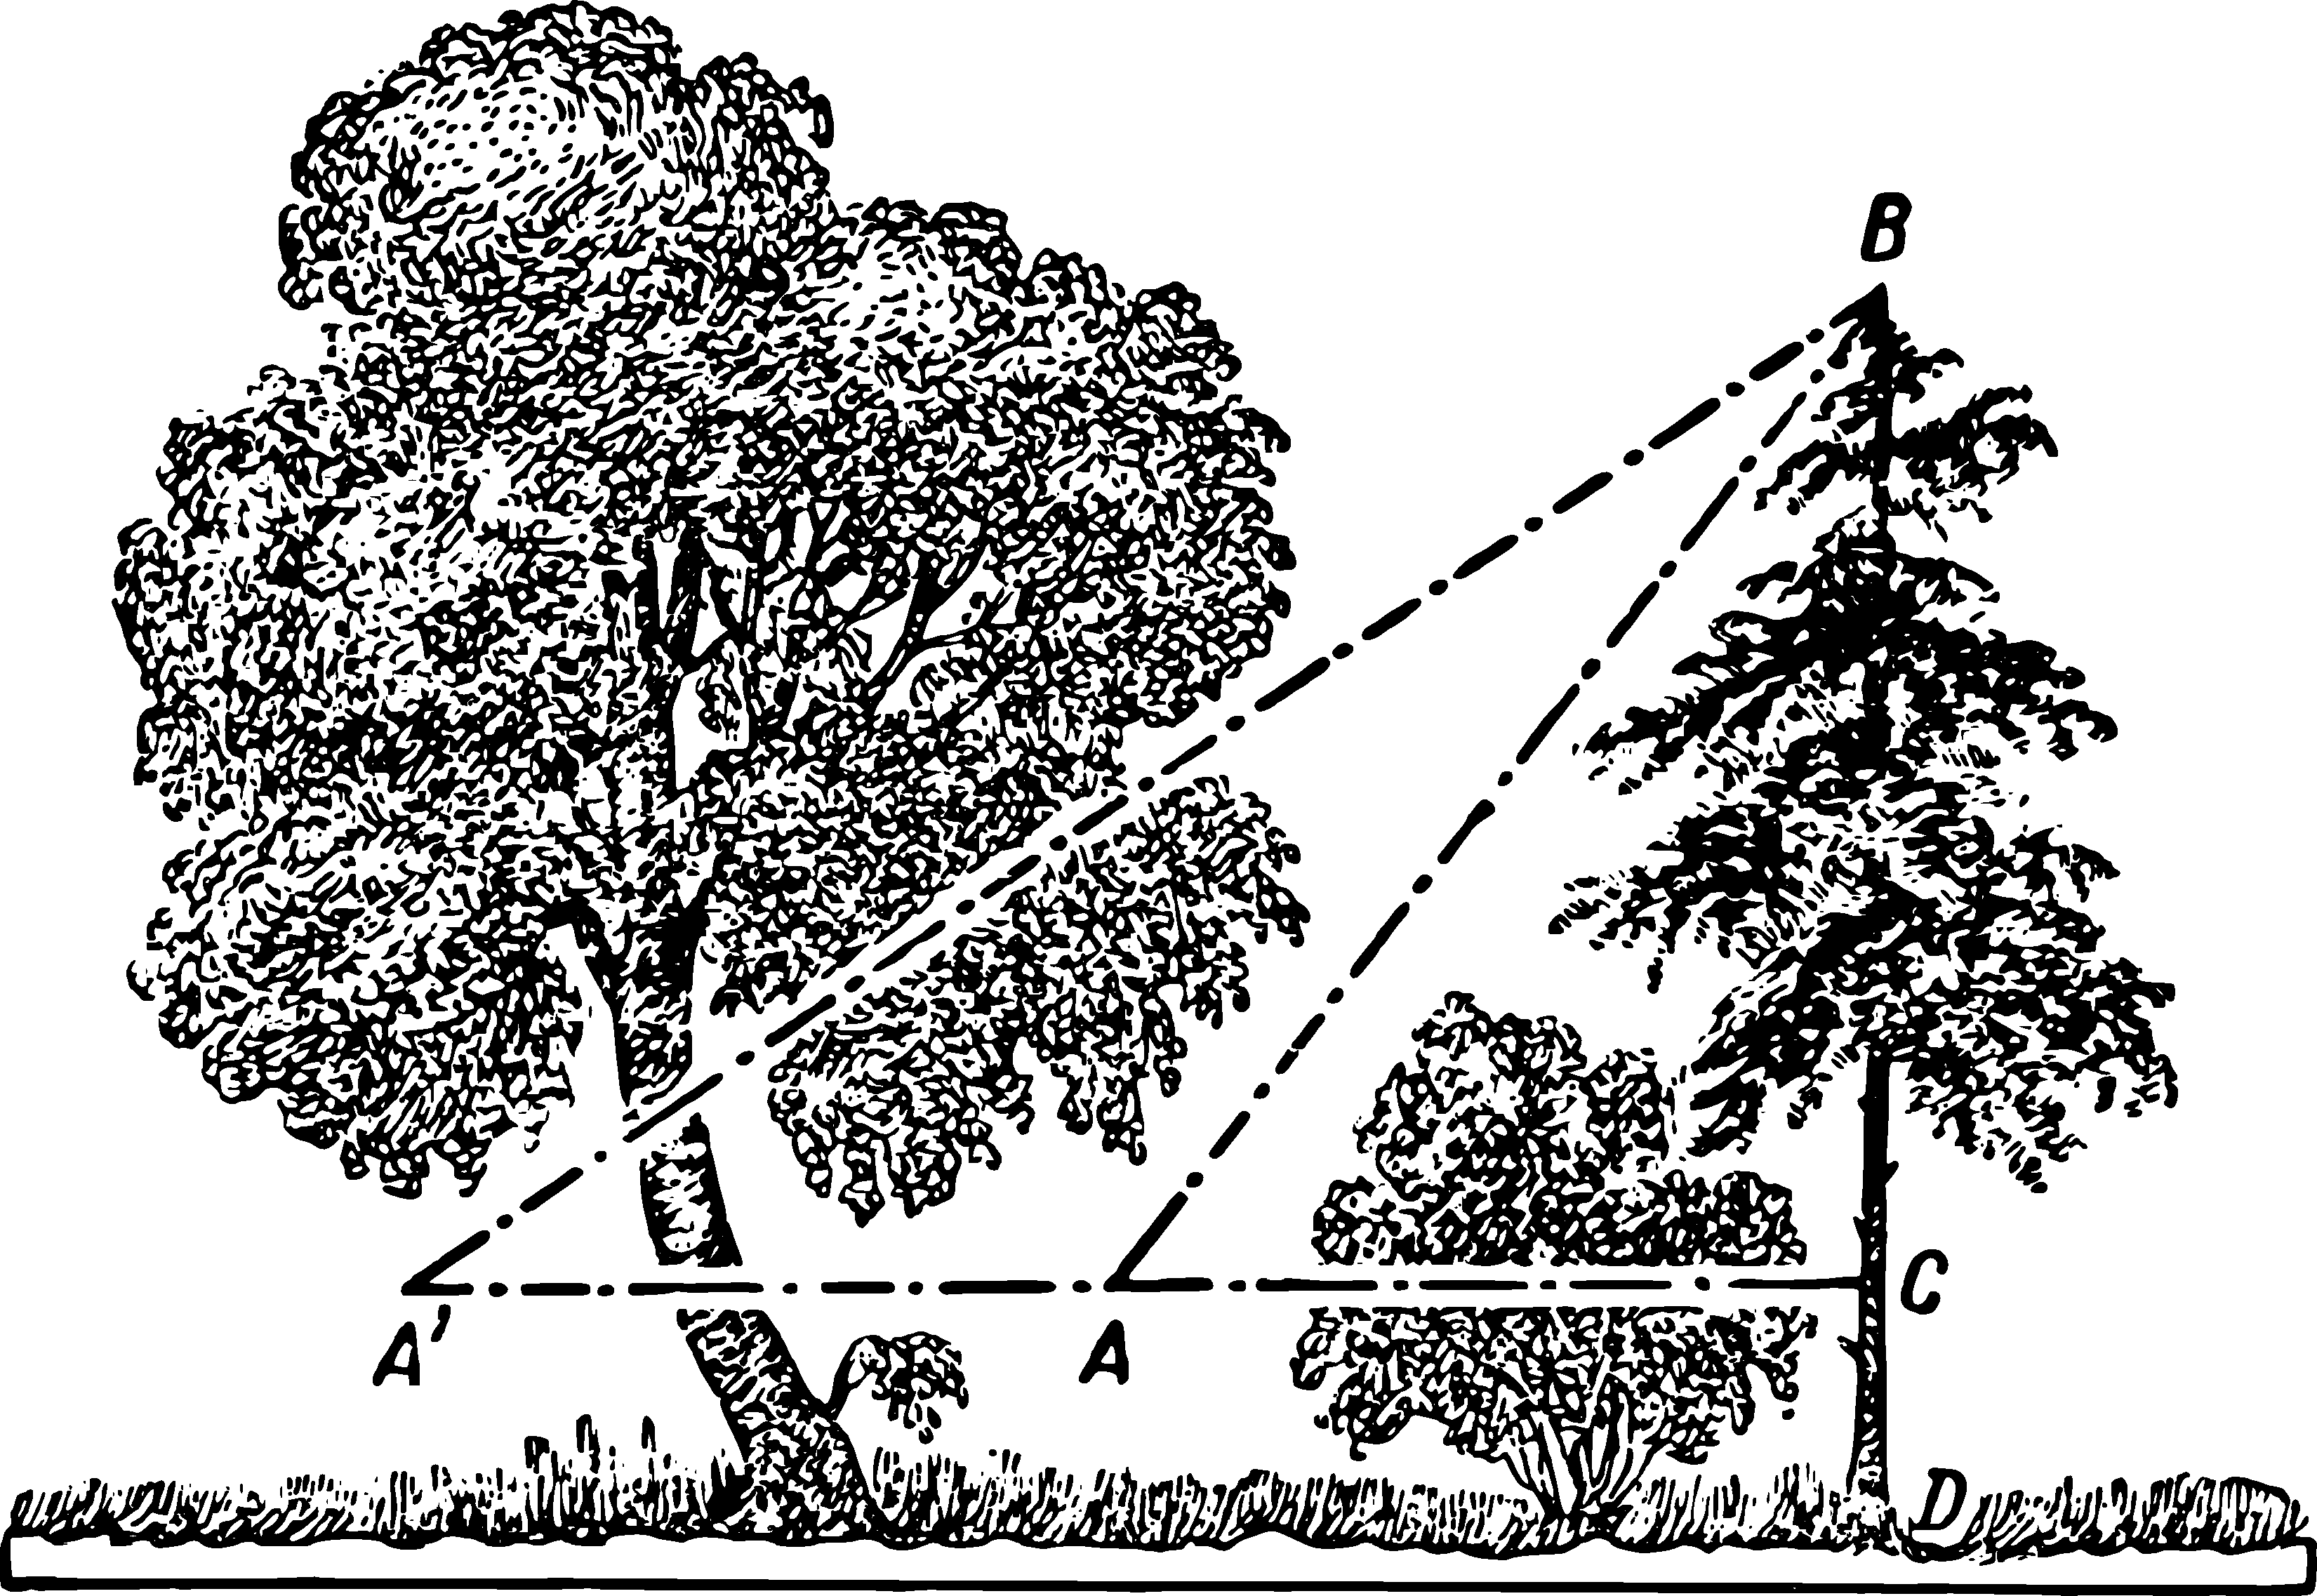
\includegraphics[width=0.9\textwidth]{figures/ch-01/fig-01-13.pdf}
\sidecaption[][-1cm]{How to measure the height of a tree without approaching it.\label{fig-01-13}}
\end{figure}

Let's say at point $A$ we determined that $BC = 0.9\,AC$, and at point $A'$ we determined that $BC = 0.4\,A'C$. Then we know that:
\begin{equation*}%
AC = \frac{BC}{0.9},\quad   A'C  = \frac{BC}{0.4} 
\end{equation*}
So that we can write
\begin{equation*}%
AA' = A'C - AC = \frac{BC}{0.4} - \frac{BC}{0.9} = \frac{25}{18} \,BC.
\end{equation*}
Hence,
\begin{align*}%
AA' & = \frac{25}{18} \,BC, \\ 
\therefore BC & = \frac{18}{25} \,AA' \\
& = 0.72 \, AA'.
\end{align*}
You can see that by measuring the distance $AA'$ between both observation points and taking a certain fraction of this value, we can determine the desired and inaccessible height.

\section{Using a Mirror}
\label{sec-1.8}


\ques Here's another unconventional method for determining the height of a tree using a mirror. At some distance (see \figr{fig-01-14}) from the tree being measured, on level ground at point $C$, place a small mirror horizontally and step back to point $D$, from where the observer can see the top of tree's point $A$ in the mirror. Then, the tree ($AB$) is as many times taller than the observer's height ($ED$) as the distance $BC$ from the mirror to the tree is greater than the distance $CD$ from the mirror to the observer. Why?

\begin{figure}[h!]
\centering
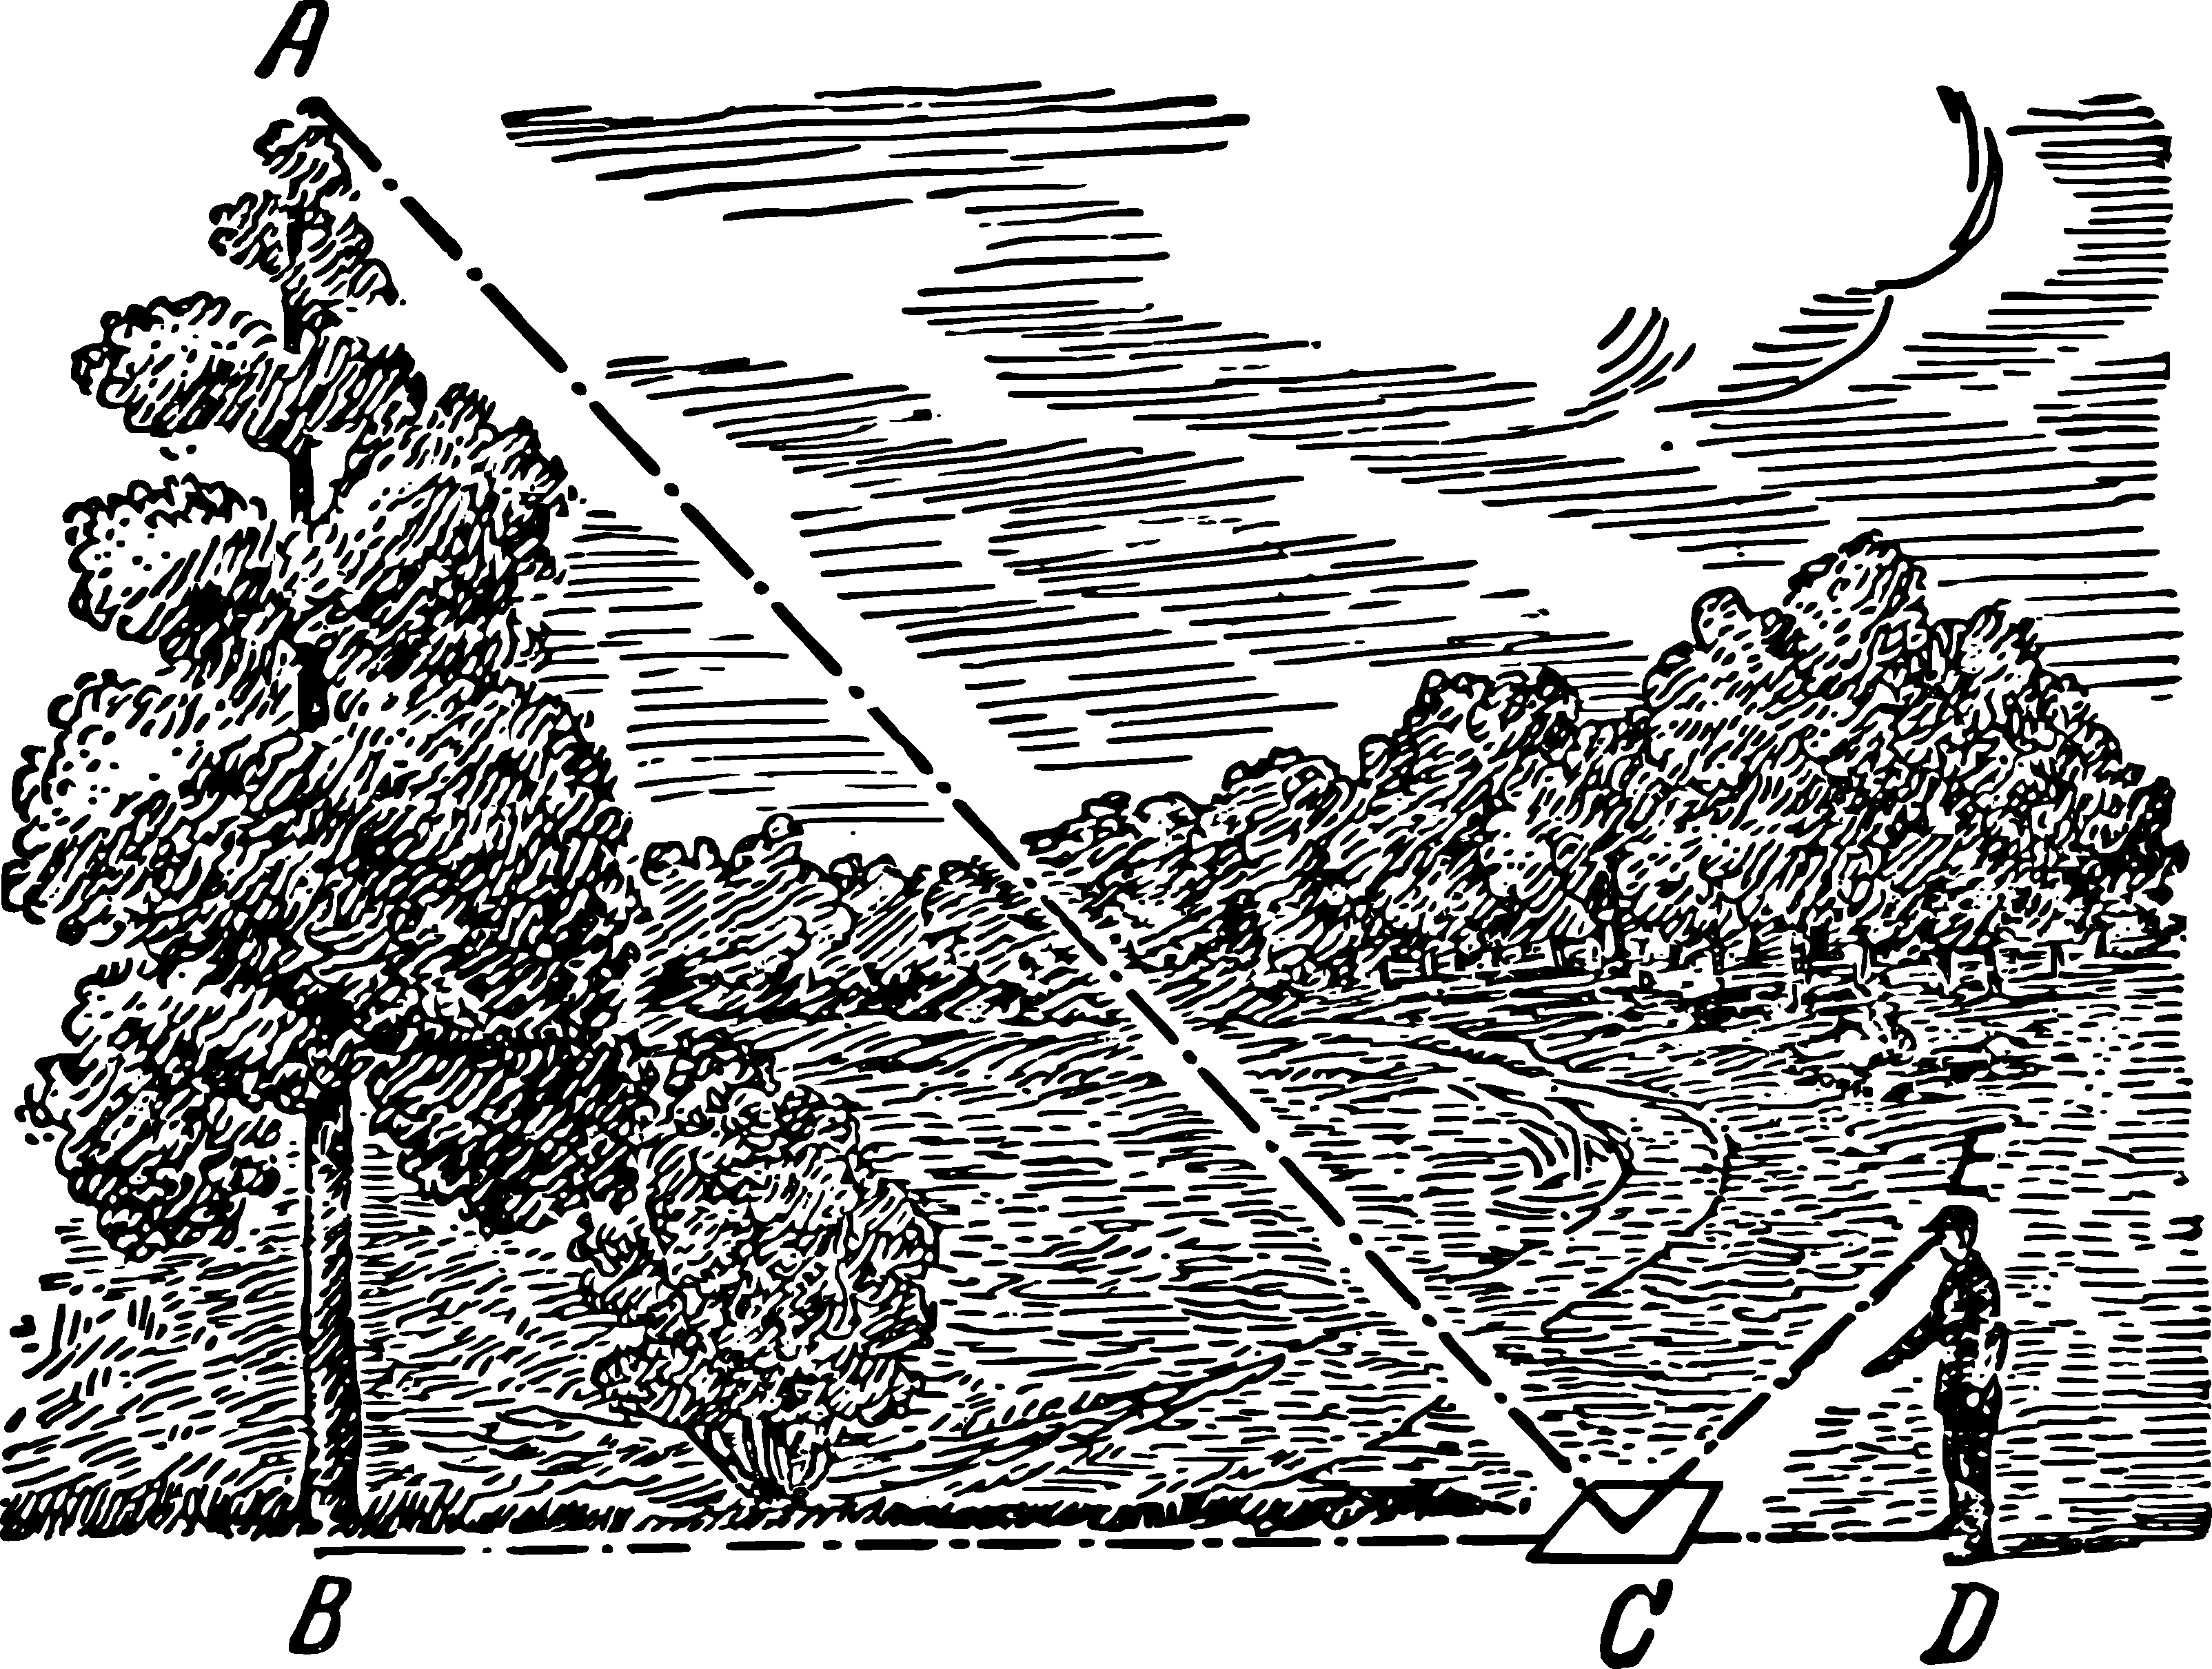
\includegraphics[width=0.9\textwidth]{figures/ch-01/fig-01-14.pdf}
\sidecaption[][0cm]{Height measurement using a mirror.\label{fig-01-14}}
\end{figure}


\ans The method is based on the law of reflection of light. The top $A$ (\figr{fig-01-15}) is reflected at point $A'$ in such a way that $AB = A'B$. From the similarity of triangles $BCA'$ and $CED$, it follows that 
\begin{equation*}%
\frac{A'B}{ED} = \frac{BC}{CD}. 
\end{equation*}
In this, simply replace $A'B$ with $AB$ to justify the relationship stated in the problem. This convenient and effortless method can be applied in any weather, but not in dense vegetation, only to a solitary tree.
\begin{marginfigure}[-4cm]%[h!]
\centering
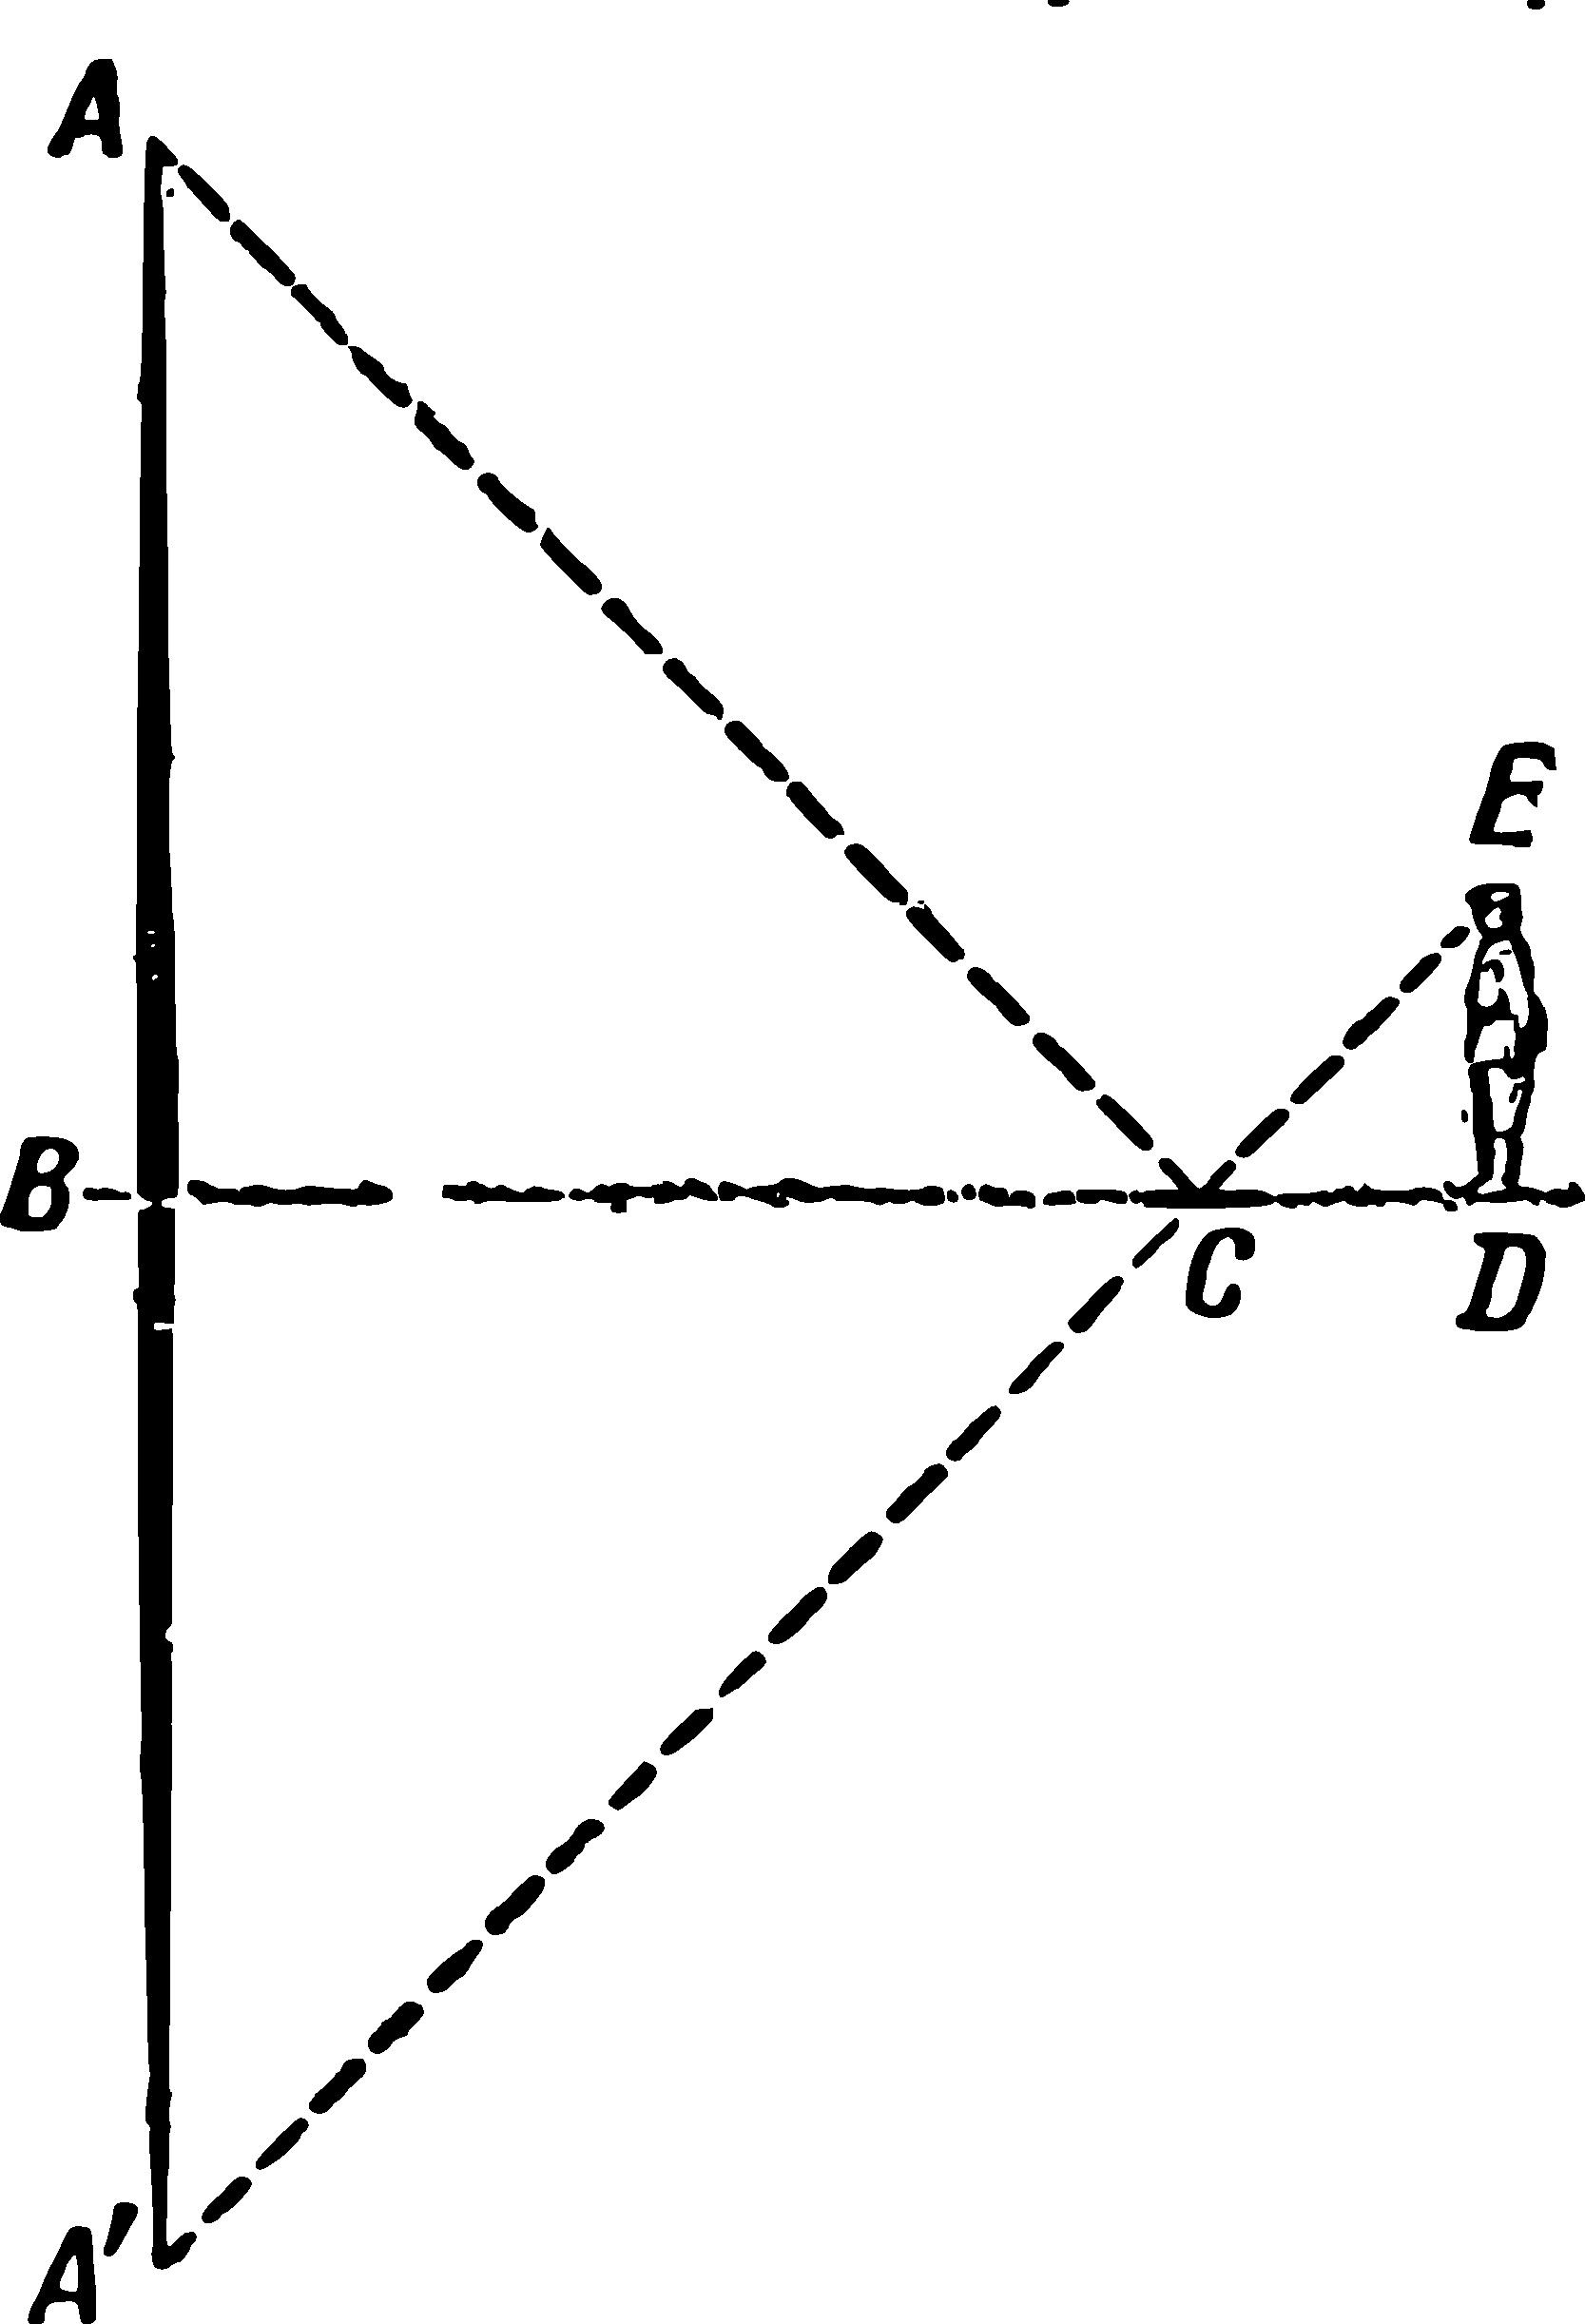
\includegraphics[width=0.9\textwidth]{figures/ch-01/fig-01-15.pdf}
\sidecaption{Geometric construction for the method of measuring the height using a mirror.\label{fig-01-15}}
\end{marginfigure}

%\clearpage 

\ques However, what should be done when it is impossible to approach the tree being measured closely for some reason?\\

\ans This is an ancient problem dating back over 500 years. It is discussed by the medieval mathematician Antonius de Cremona in his work \emph{On Practical Land Measurement} (1400).


The problem is solved by the dual application of the method described earlier -- placing the mirror in two locations. By making the appropriate construction, it is easy to deduce from the similarity of triangles that the sought-after height of the tree is equal to the observer's eye level multiplied by the ratio of the distance between the mirror positions to the difference in distances from the mirror to the observer.

Before concluding the discussion on measuring the height of trees, I propose to the reader another ``forest'' problem.

\section{Two Pines}
\label{sec-1.9}


\ques Two pine trees grow 40 meters apart. You measured their heights: one turned out to be 31 meters tall, while the other, younger one, is only 6 meters tall. Can you calculate the distance between their tops?

\begin{figure}[h!]
\centering
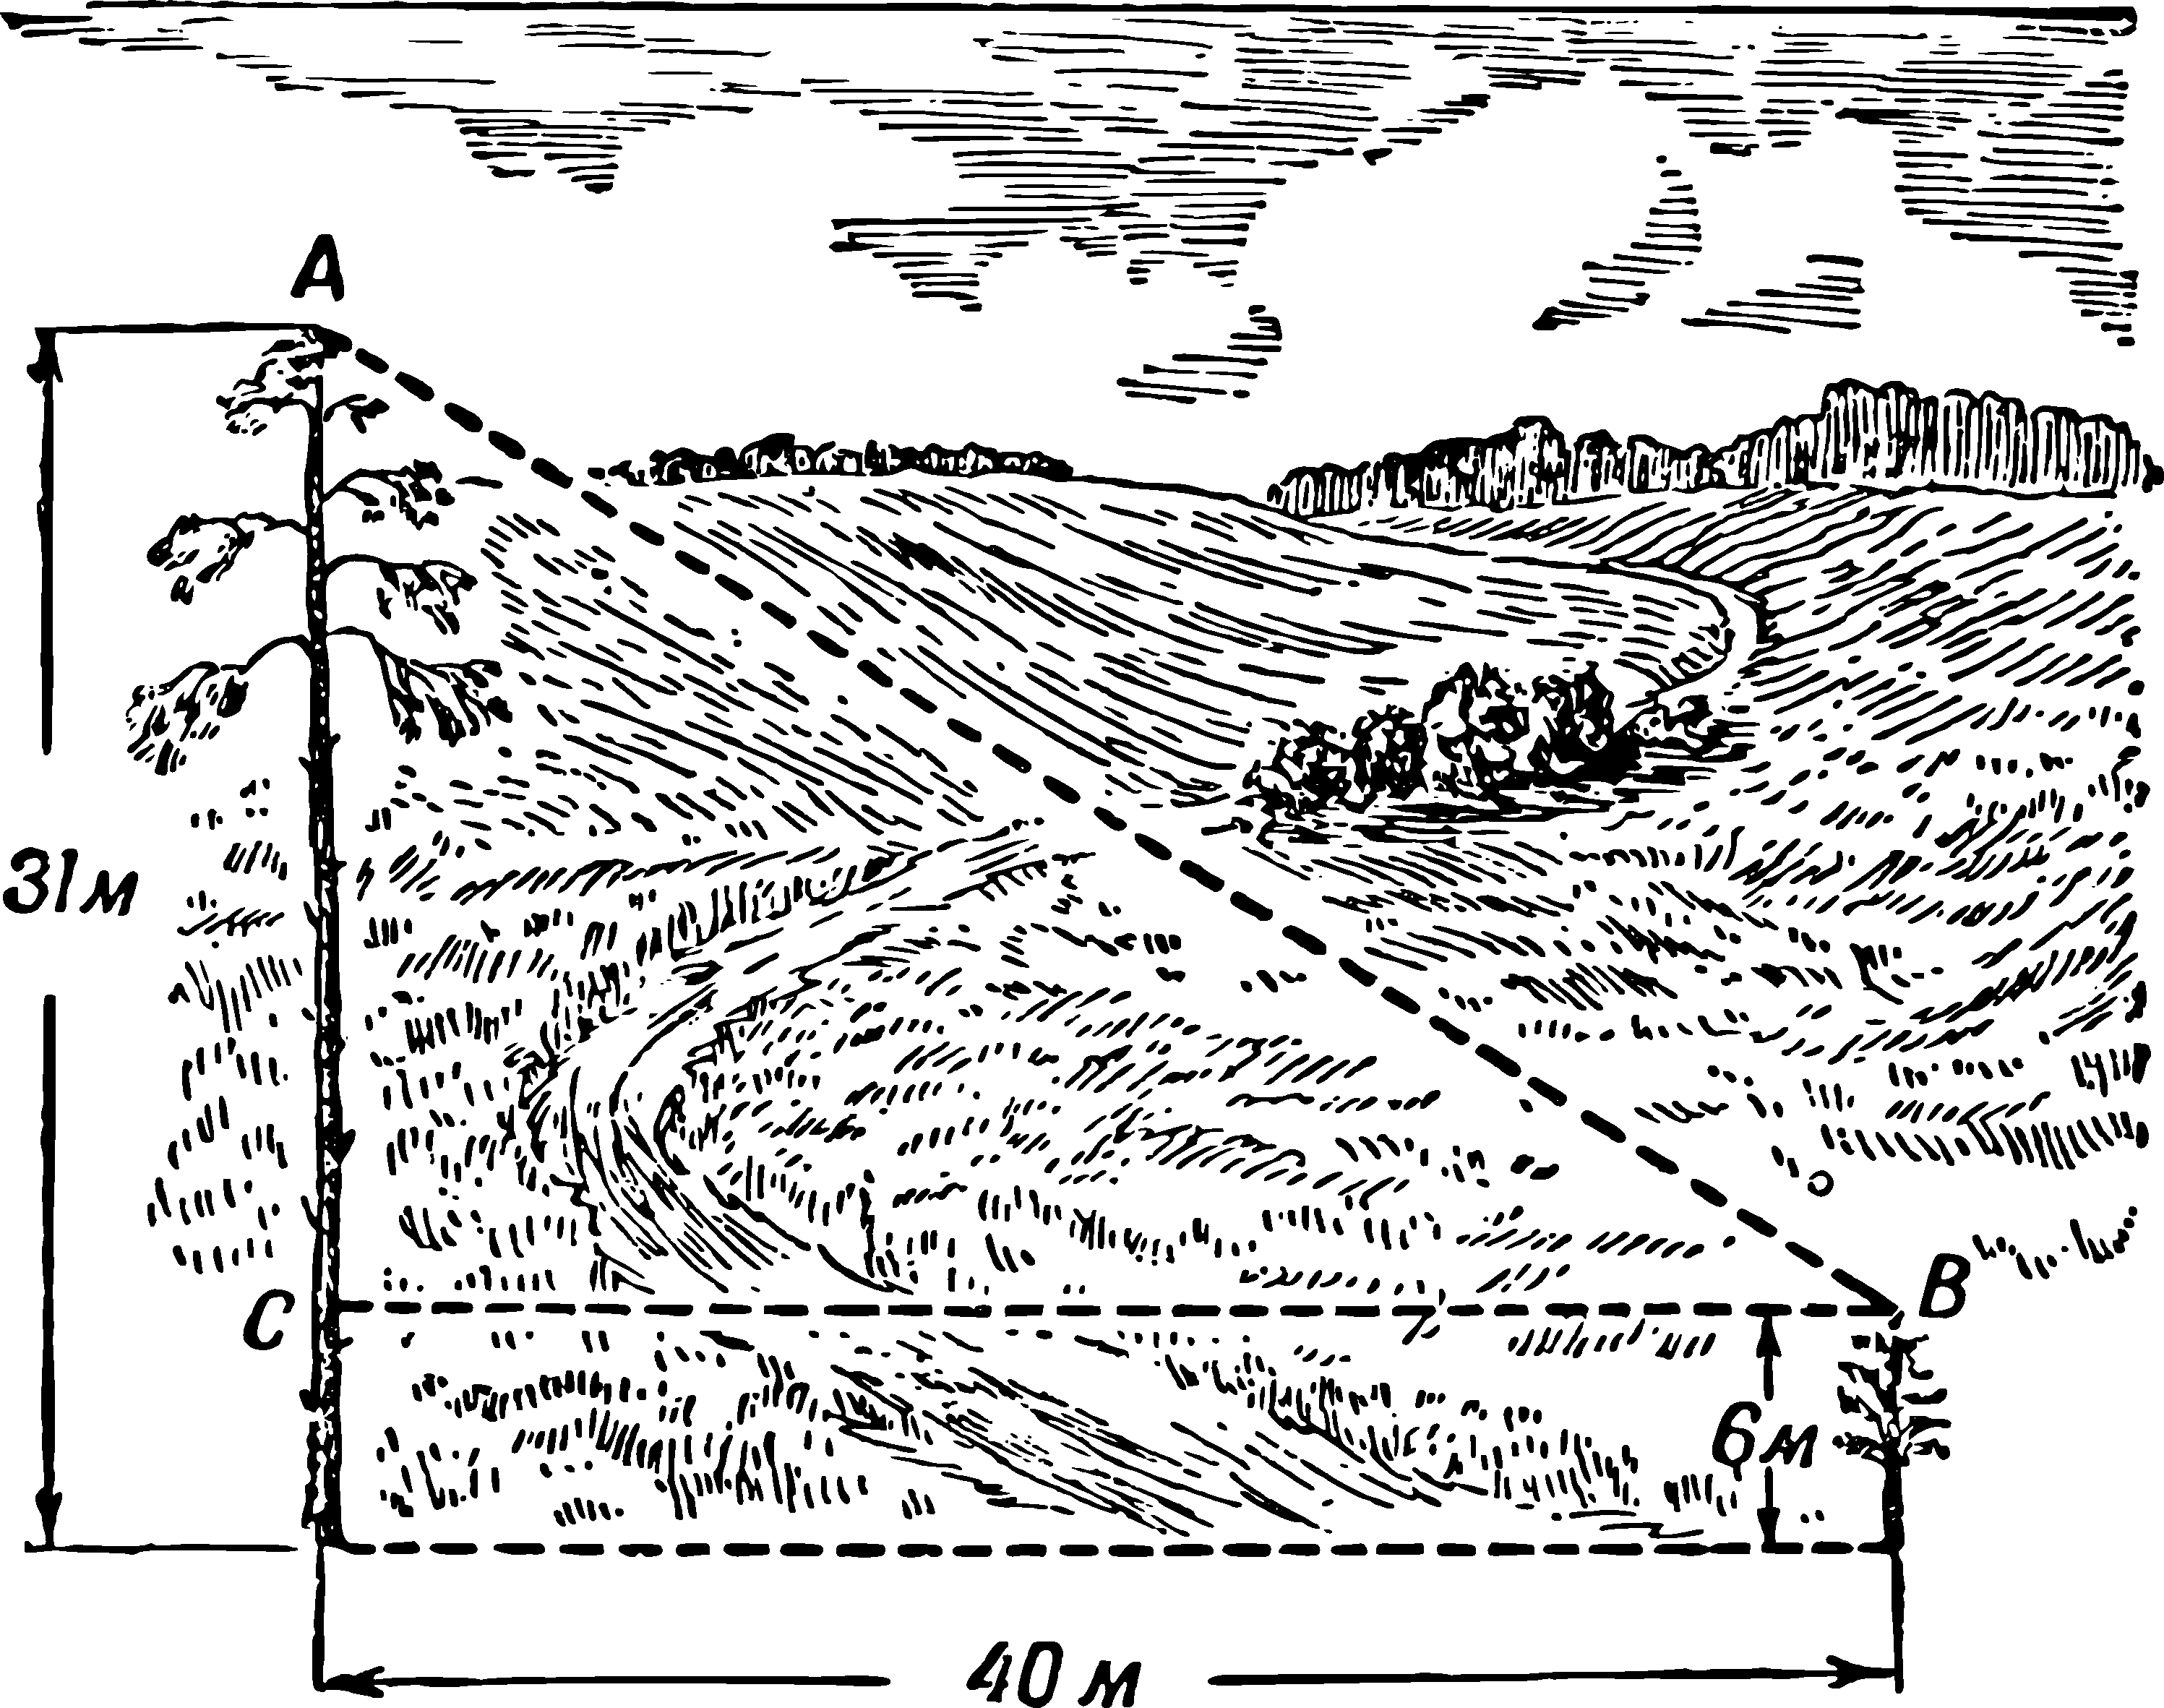
\includegraphics[width=0.9\textwidth]{figures/ch-01/fig-01-16.pdf}
\sidecaption{What is the distance between the tops of the pines?\label{fig-01-16}}
\end{figure}

\ans The desired distance between the tops of the pine trees (see \figr{fig-01-16}) according to the Pythagorean theorem is
\begin{equation*}%
\sqrt{40^{2} + 25^{2}} = \SI{47}{\meter}.
\end{equation*}



\section{The shape of the tree trunk}
\label{sec-1.10}

Now you can already, walking through the forest, determine -- in almost half a dozen different ways -- the height of any tree. It will probably be interesting for you to determine its volume as well, calculate how many cubic meters of wood it contains, and at the same time weigh it. To find out if, for example, it would be possible to take away such a trunk on one cart. Both of these tasks are no longer as simple as determining height; experts have not found ways to accurately resolve it and are content with only a more or less approximate estimate. Even for a felled trunk, which lies in front of you cleared of branches, the task is far from easy.

The thing is, a tree trunk, even the smoothest one without bulges, does not represent either a cylinder, a complete cone, a truncated cone, or any other geometric solid whose volume we can calculate using formulas. The trunk is certainly not a cylinder — it tapers towards the top (it has ``runoff'', as foresters say) — but it is also not a cone because its ``generating line'' is not a straight line, but a curve, and moreover, not a circular arc, but some other curve, convex towards the axis of the tree.\sidenote[][-5cm]{The curve that fits closest to this is called the ``semicubical parabola'' $(y^3 = ax^2)$; the solid obtained by rotating this parabola is called a ``neiloid'' (named after the ancient mathematician Neil, who found a way to determine the length of the arc of such a curve). The shape of a tree trunk grown in the forest approximates that of a neiloid. Calculating the volume of a neiloid is done using advanced mathematical techniques.}

Therefore, a more or less accurate calculation of the volume of a tree trunk can only be done using the tools of integral calculus. To some readers, it may seem strange that the measurement of a simple log requires resorting to the services of higher mathematics. Many think that higher mathematics is only relevant to some special subjects, whereas in everyday life, only elementary mathematics is applicable. This is completely incorrect: one can fairly accurately calculate the volume of a star or a planet using elements of geometry, whereas an exact calculation of the volume of a long log or a beer barrel is impossible without analytical geometry and integral calculus.

However, our book does not assume that the reader is familiar with higher mathematics; therefore, here we will have to be content with only an approximate calculation of the volume of the trunk. We will assume that the volume of the trunk is more or less close either to the volume of a truncated cone, or -- for a trunk with a pointed end — to the volume of a complete cone, or, finally, -- for short logs — to the volume of a cylinder. The volume of each of these three solids can be easily calculated. Could we find a formula for the volume that would be suitable for all three of these named solids for the sake of consistency in calculation? Then we would approximately calculate the volume of the trunk without caring about what it resembles more — a cylinder or a cone, complete or truncated.


\section{Universal Formula}
\label{sec-1.11}

Such a formula exists; moreover, it is not only suitable for cylinders, complete and truncated cones, but also for all kinds of prisms, pyramids complete and truncated, and even for spheres. Here is this remarkable formula, known in mathematics as Simpson's formula:
\begin{equation*}
v = \frac{h}{6}\, (b_{1} + 4b_{2} + b_{3})
\end{equation*}
where $h$ is the height of the solid, $b_{1}$ is the area of the lower base, $b_{2}$ is the area of the middle section\sidenote[][-2cm]{ That is, the cross-sectional area of the body in the middle of its height.}, $b_{3}$ is the area of the upper base.

\ques Prove that with this formula, one can calculate the volume of the following seven geometric solids: prism, pyramid complete, pyramid truncated, cylinder, cone complete, cone truncated, sphere.

\ans It is very easy to verify the correctness of this formula by simply applying it to the listed solids. Then, we obtain for the prism and cylinder (see \figr{fig-01-17}~\drkgry{a}):
\begin{equation*}%
v = \frac{h}{6}\, (b_{1} + 4b_{2} + b_{3}) = b_{1}h;
\end{equation*}
for the pyramid and cone (see \figr{fig-01-17}~\drkgry{b}):
\begin{equation*}%
v = \frac{h}{6}\, (b_{1} + 4\frac{b_{2}}{4} + 0) = \frac{b_{1}h}{3};
\end{equation*}
for the truncated cone (see \figr{fig-01-17}~\drkgry{c}):
\begin{align*}%
v & = \frac{h}{6}\, \left[ \pi R^{2} + 4 \pi \frac{(R + r)^{2}}{2} + \pi r^{2} \right] \\ 
& = \frac{h}{6}\, \left[ \pi R^{2} + \pi R^{2} + 2 \pi Rr +  \pi r^{2} + \pi r^{2} \right] \\ 
& = \frac{\pi h}{3}\, \left[ R^{2} + Rr + r^{2}\right],
\end{align*}
for the truncated pyramid, the proof proceeds similarly; finally, for the sphere (see \figr{fig-01-17}~\drkgry{d}):
\begin{equation*}%
v = \frac{2R}{6}\, (0 + 4 \pi R^{2}{4} + 0) = \frac{4}{3}\pi R^{3}.
\end{equation*}

\begin{figure}[h!]
\centering
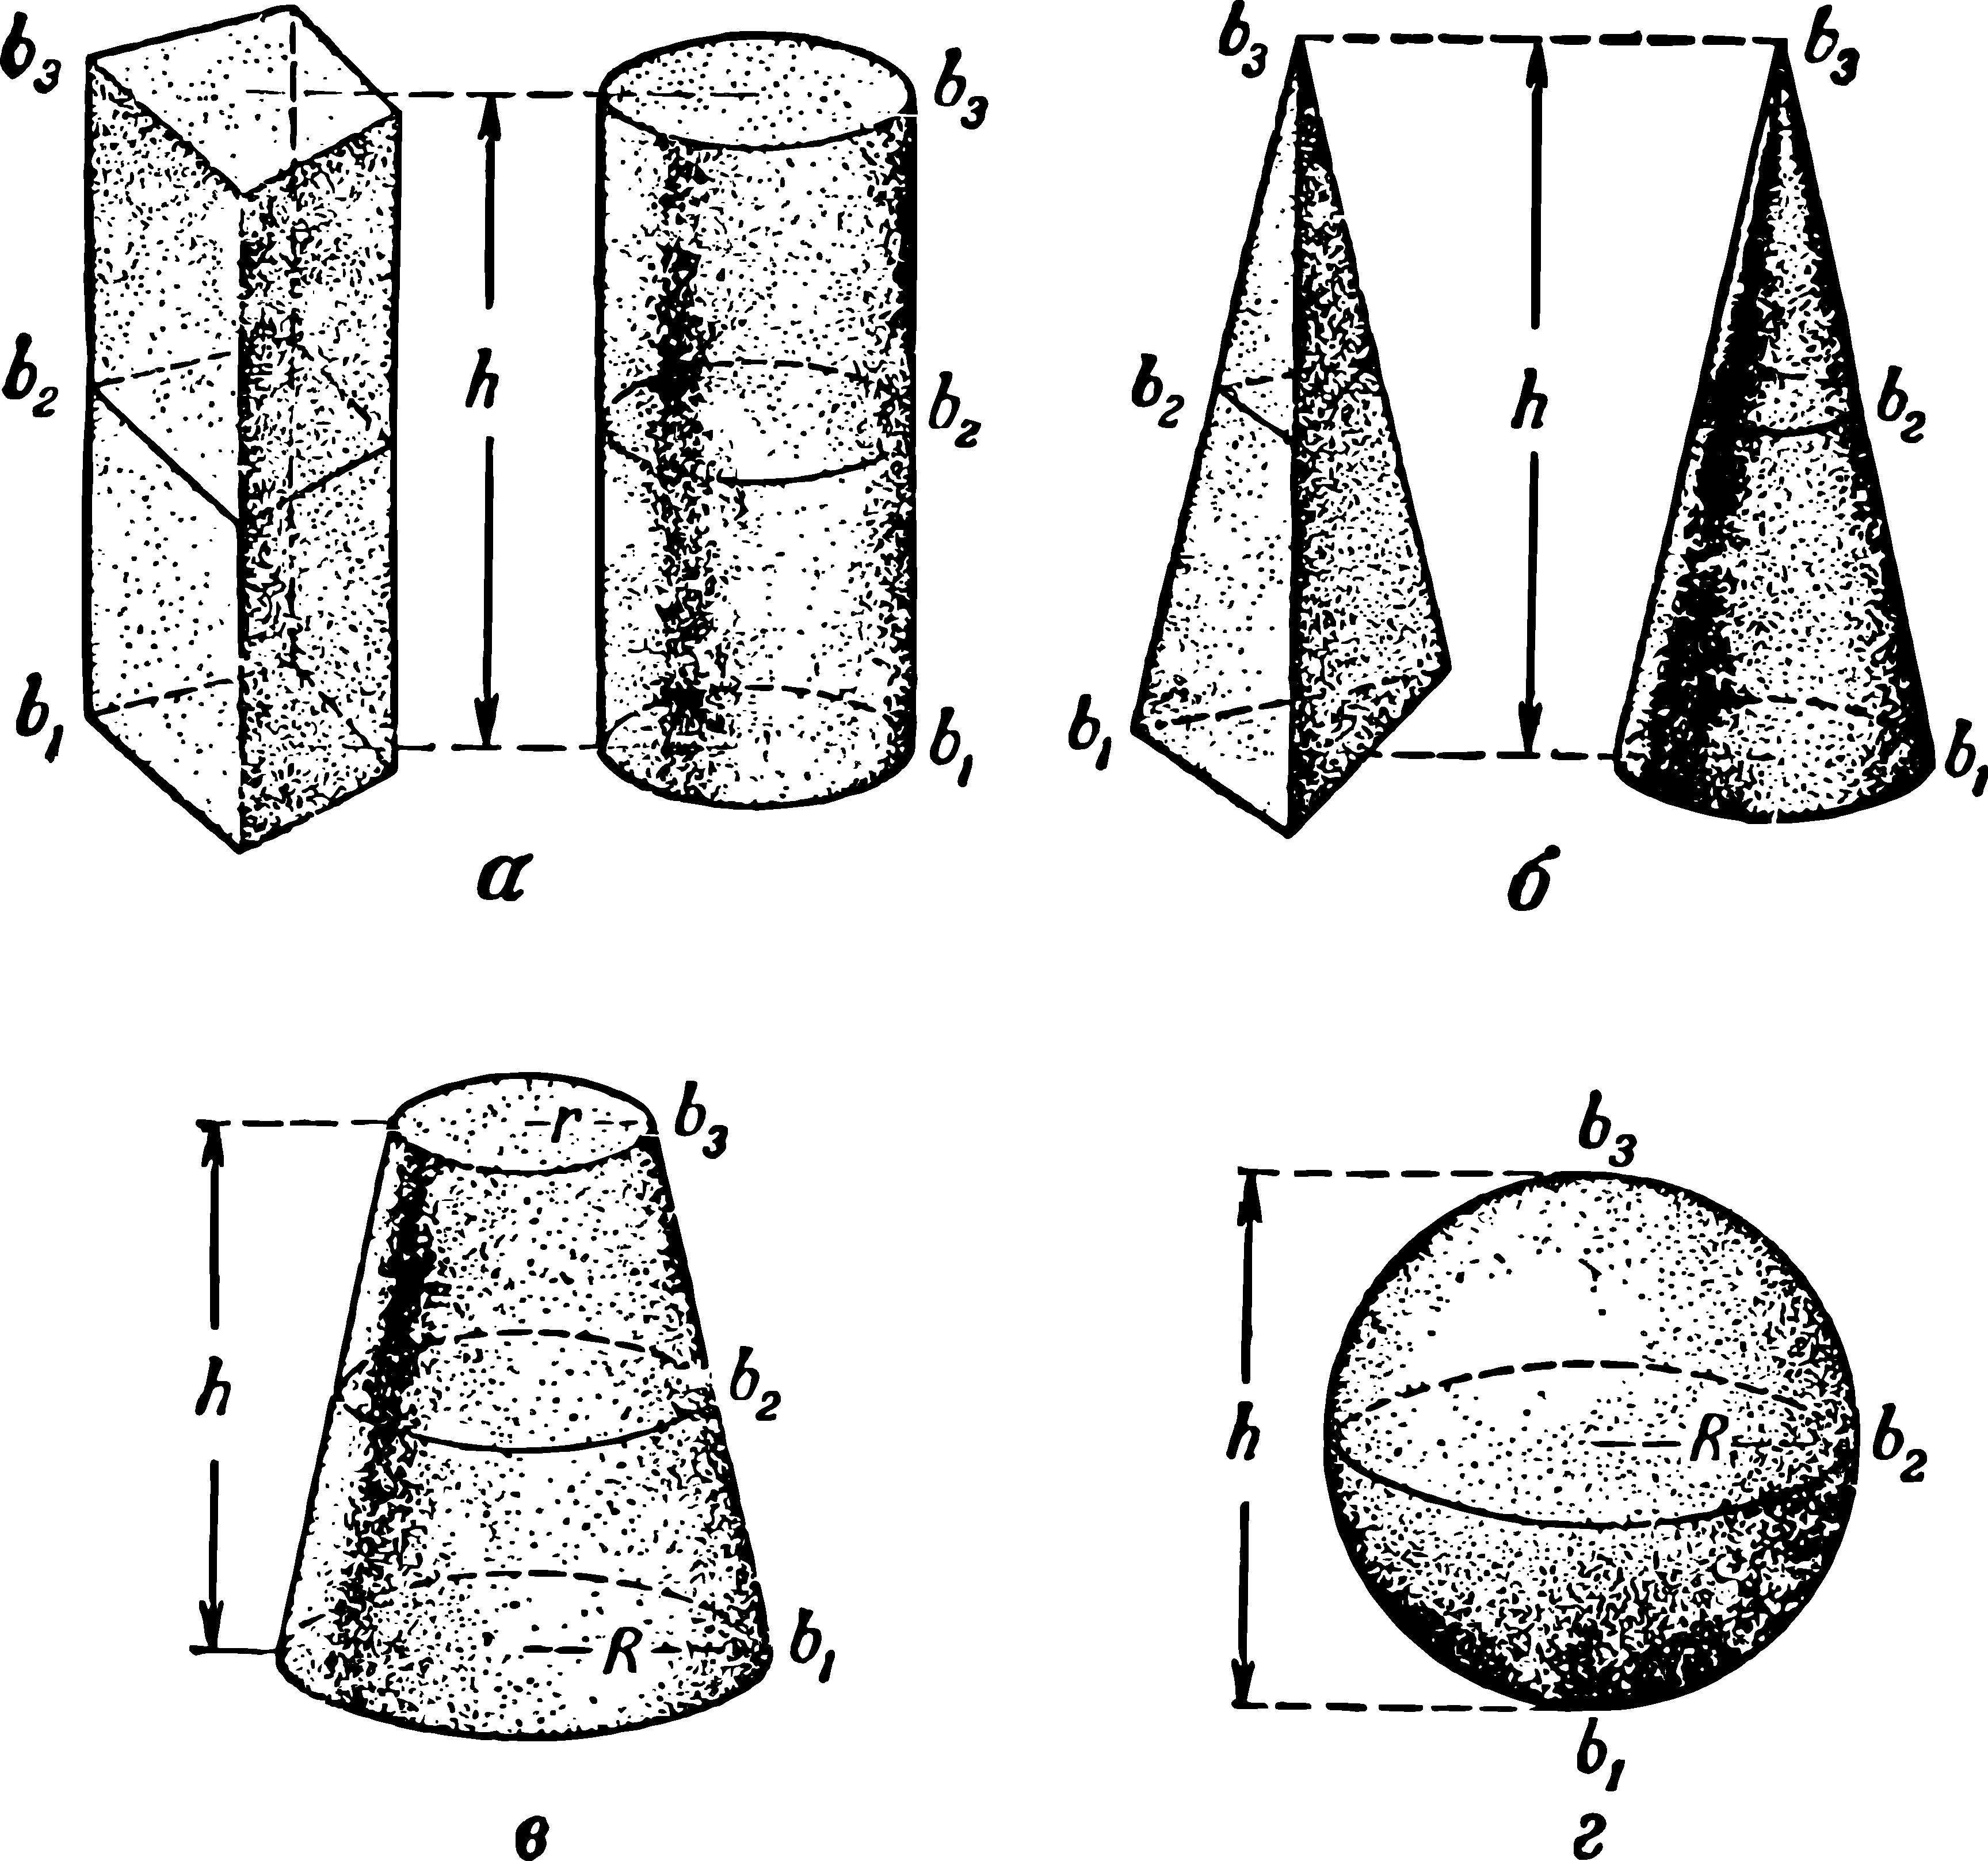
\includegraphics[width=0.9\textwidth]{figures/ch-01/fig-01-17.pdf}
\sidecaption[][-2cm]{Geometric bodies whose volumes can be calculated using a single formula.\label{fig-01-17}}
\end{figure}

\ques Let's note another interesting feature of our universal formula: it is also suitable for calculating the area of plane figures: parallelograms, trapezoids, and triangles, if by 
\begin{enumerate}[label=\textsection]
\item \( h \) we mean, as before, the height of the figure, 
\item by \( b_{1} \) the length of the lower base, 
\item by \( b_{2} \) the length of the middle base and 
\item by $b_{3}$ the length of the lower base. 
\end{enumerate}
How can we confirm this?

\ans Applying the formula, we have: for a parallelogram (square, rectangle) (see \figr{fig-01-18}~\drkgry{a})
\begin{equation*}%
S = \frac{h}{6}\, (b_{1} + 4 b_{1} + b_{1}) = b_{1}h;
\end{equation*}
for a trapezoid (see \figr{fig-01-18}~\drkgry{b})
\begin{equation*}%
S = \frac{h}{6}\, \left( b_{1} + 4 \frac{b_{1} + b_{2}}{2} + b_{3} \right) = \frac{h}{2}\,(b_{1} + b_{3});
\end{equation*}
for a triangle (see \figr{fig-01-18}~\drkgry{c})
\begin{equation*}%
S = \frac{h}{6}\, \left( b_{1} + 4 \frac{b_{1}}{2} + 0 \right) = \frac{b_{1}h}{2}.
\end{equation*}
You can see that our formula has enough right to be called universal.

\begin{figure}[h!]
\centering
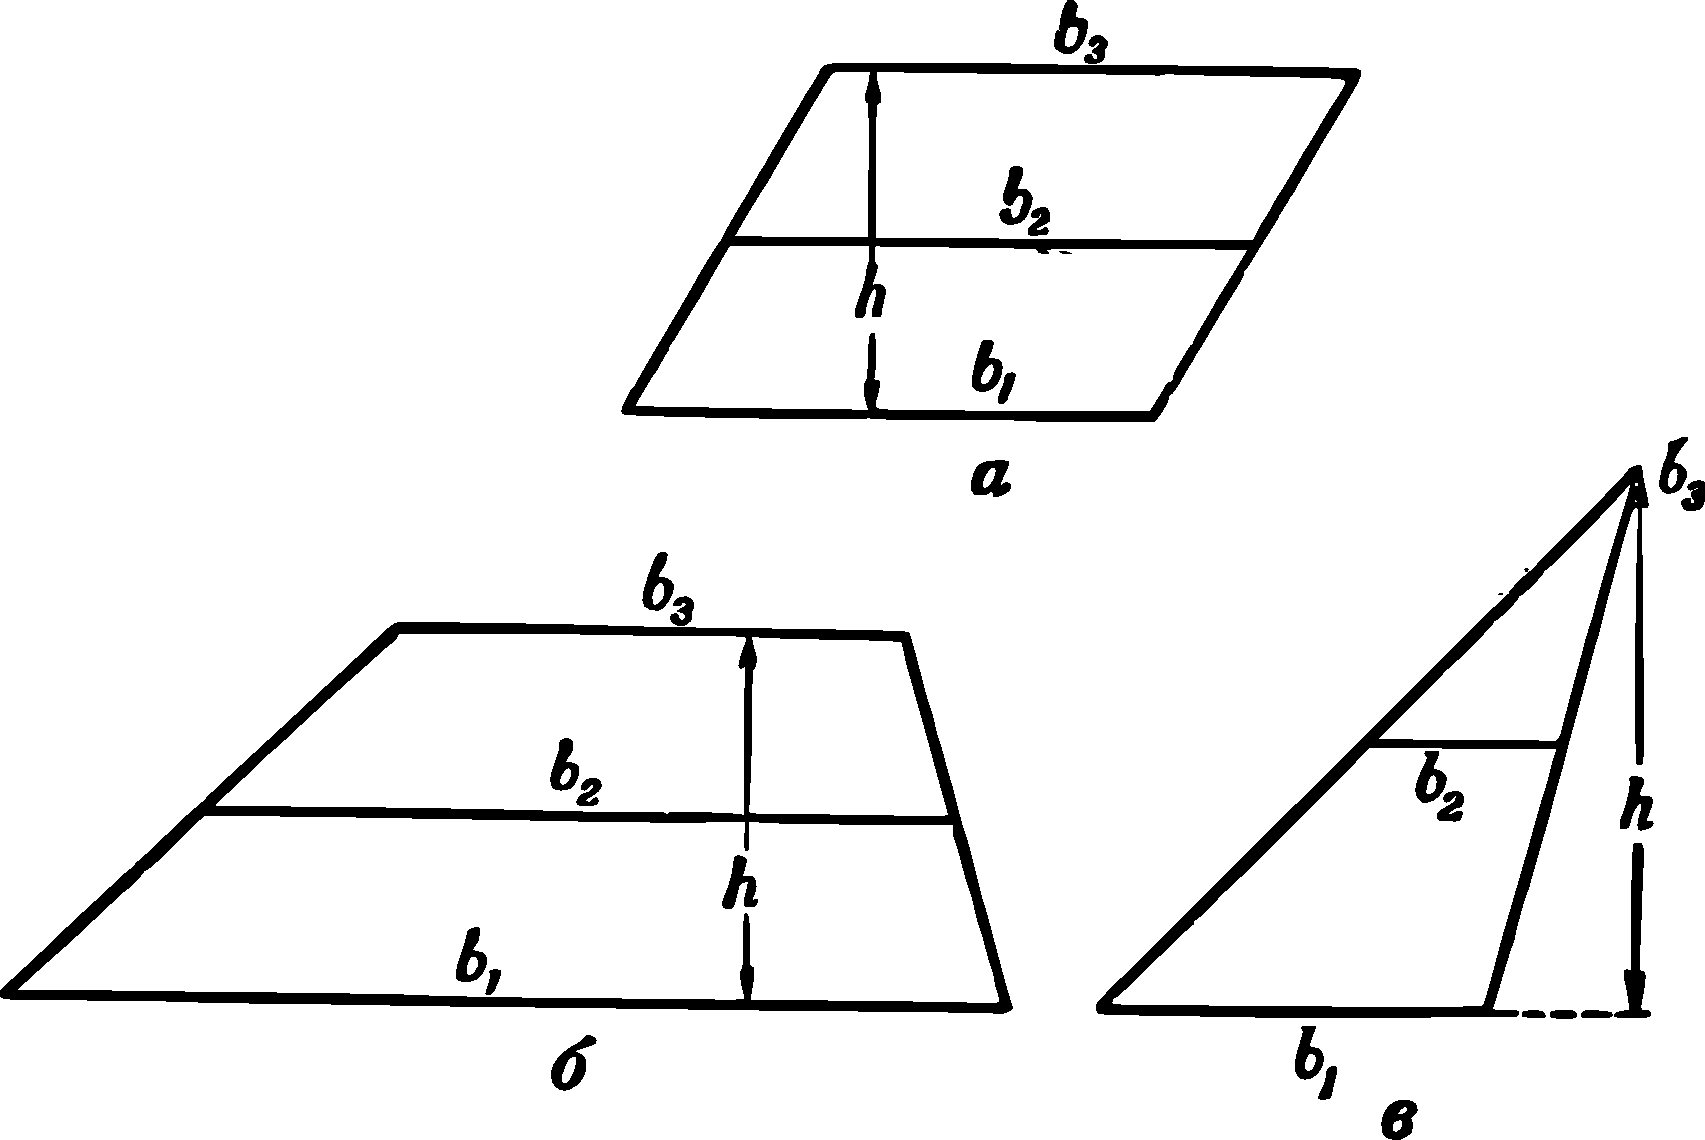
\includegraphics[width=\textwidth]{figures/ch-01/fig-01-18.pdf}
\sidecaption{The universal formula is also suitable for calculating the areas of these figures.\label{fig-01-18}}
\end{figure}


\section{Volume and Weight of a Tree at the Root}
\label{sec-1.12}

So, you have a formula with which you can approximately calculate the volume of a felled tree trunk without worrying about what geometric shape it resembles: a cylinder, a complete cone, or a truncated cone. For this, four measurements are needed -- the length of the trunk and three diameters: the lower cut, the upper, and in the middle of the length. Measuring the lower and upper diameters is very simple; however, determining the average diameter without a special device (``measuring fork'' used by foresters, see \figr{fig-01-19} and \figr{fig-01-20}\sidenote{A similar principle is applied in the well-known device for measuring the diameter of round objects -- the caliper \figr{fig-01-20}, to the right).} is quite difficult. But the difficulty can be overcome by encircling the trunk with a rope and dividing its length by 3 1/7 to get the diameter.

\begin{figure}[h!]
\centering
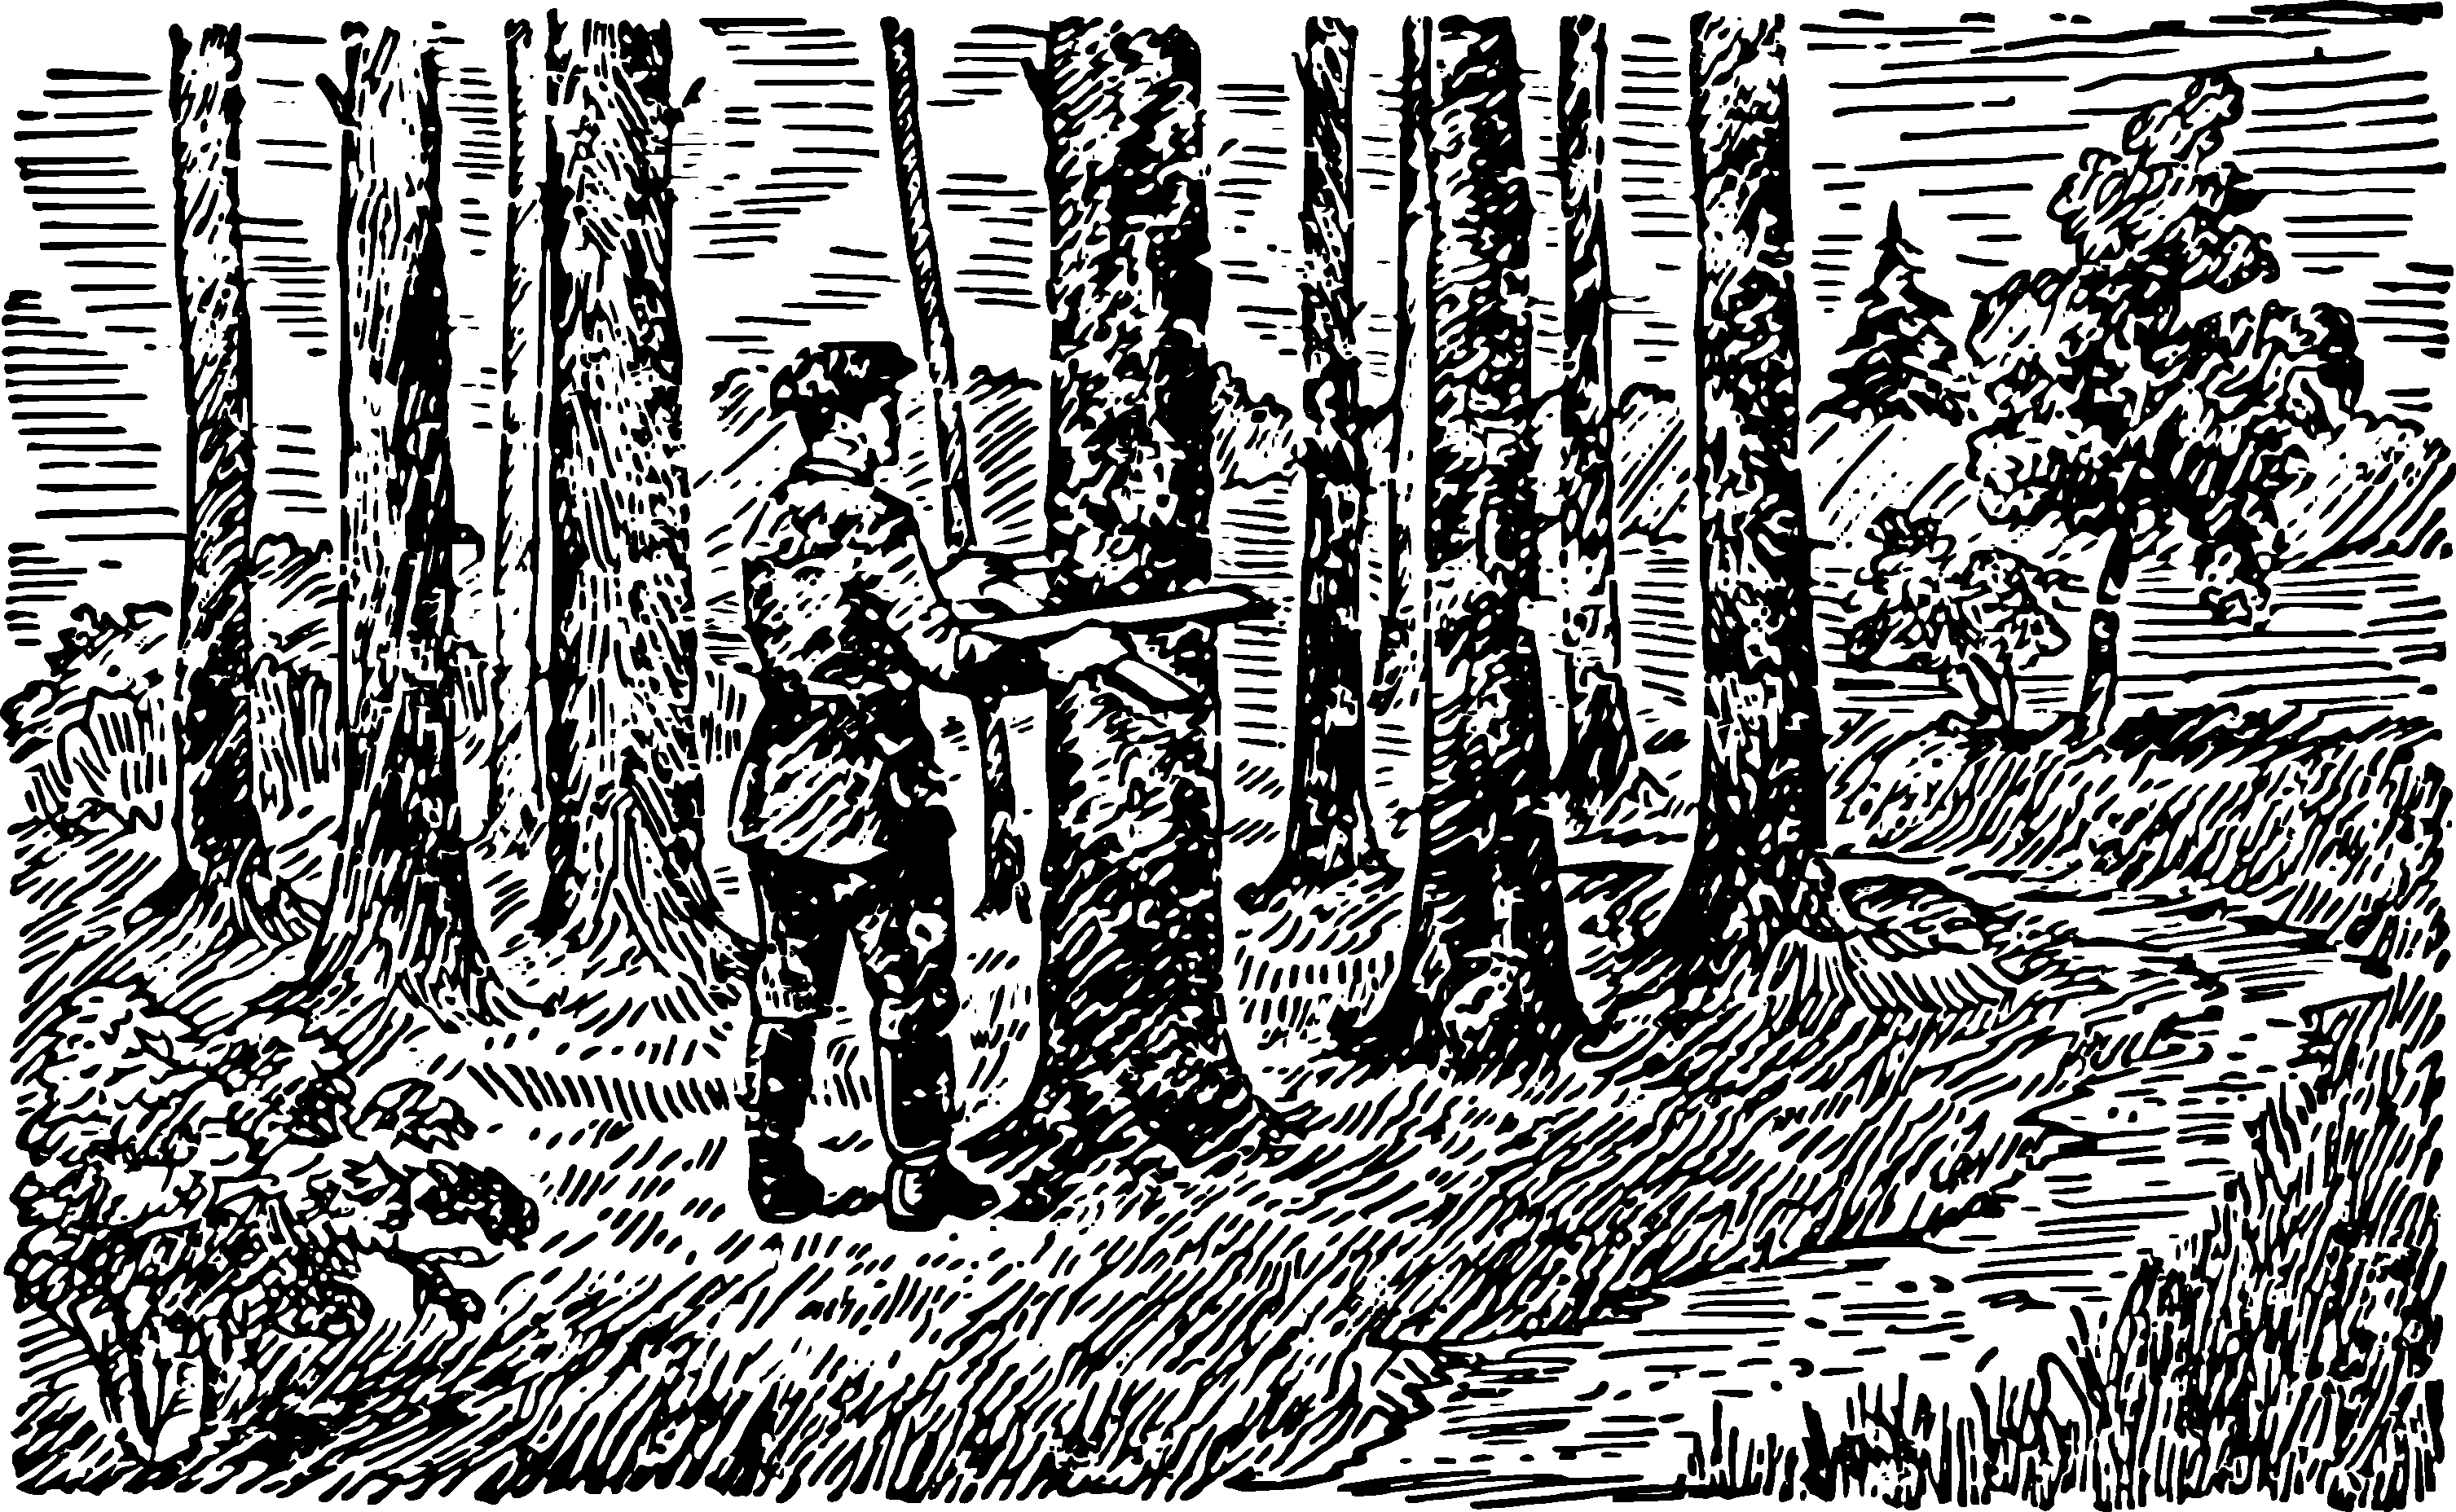
\includegraphics[width=\textwidth]{figures/ch-01/fig-01-19.pdf}
\sidecaption{Measuring the diameter of a tree with a measuring fork.\label{fig-01-19}}
\end{figure}


The volume of a felled tree trunk obtained in this way is accurate enough for many practical purposes. In short, but less accurately, this problem can be solved by calculating the volume of the trunk as the volume of a cylinder, the diameter of the base of which is equal to the diameter of the trunk in the middle of its length; however, the result obtained is underestimated, sometimes by 12\%. But if you mentally divide the trunk into two-meter segments and determine the volume of each of these almost cylindrical parts to then add them up, the result will be much better: it errs on the side of underestimation by no more than 2–3\%.

\begin{figure}[h!]
\centering
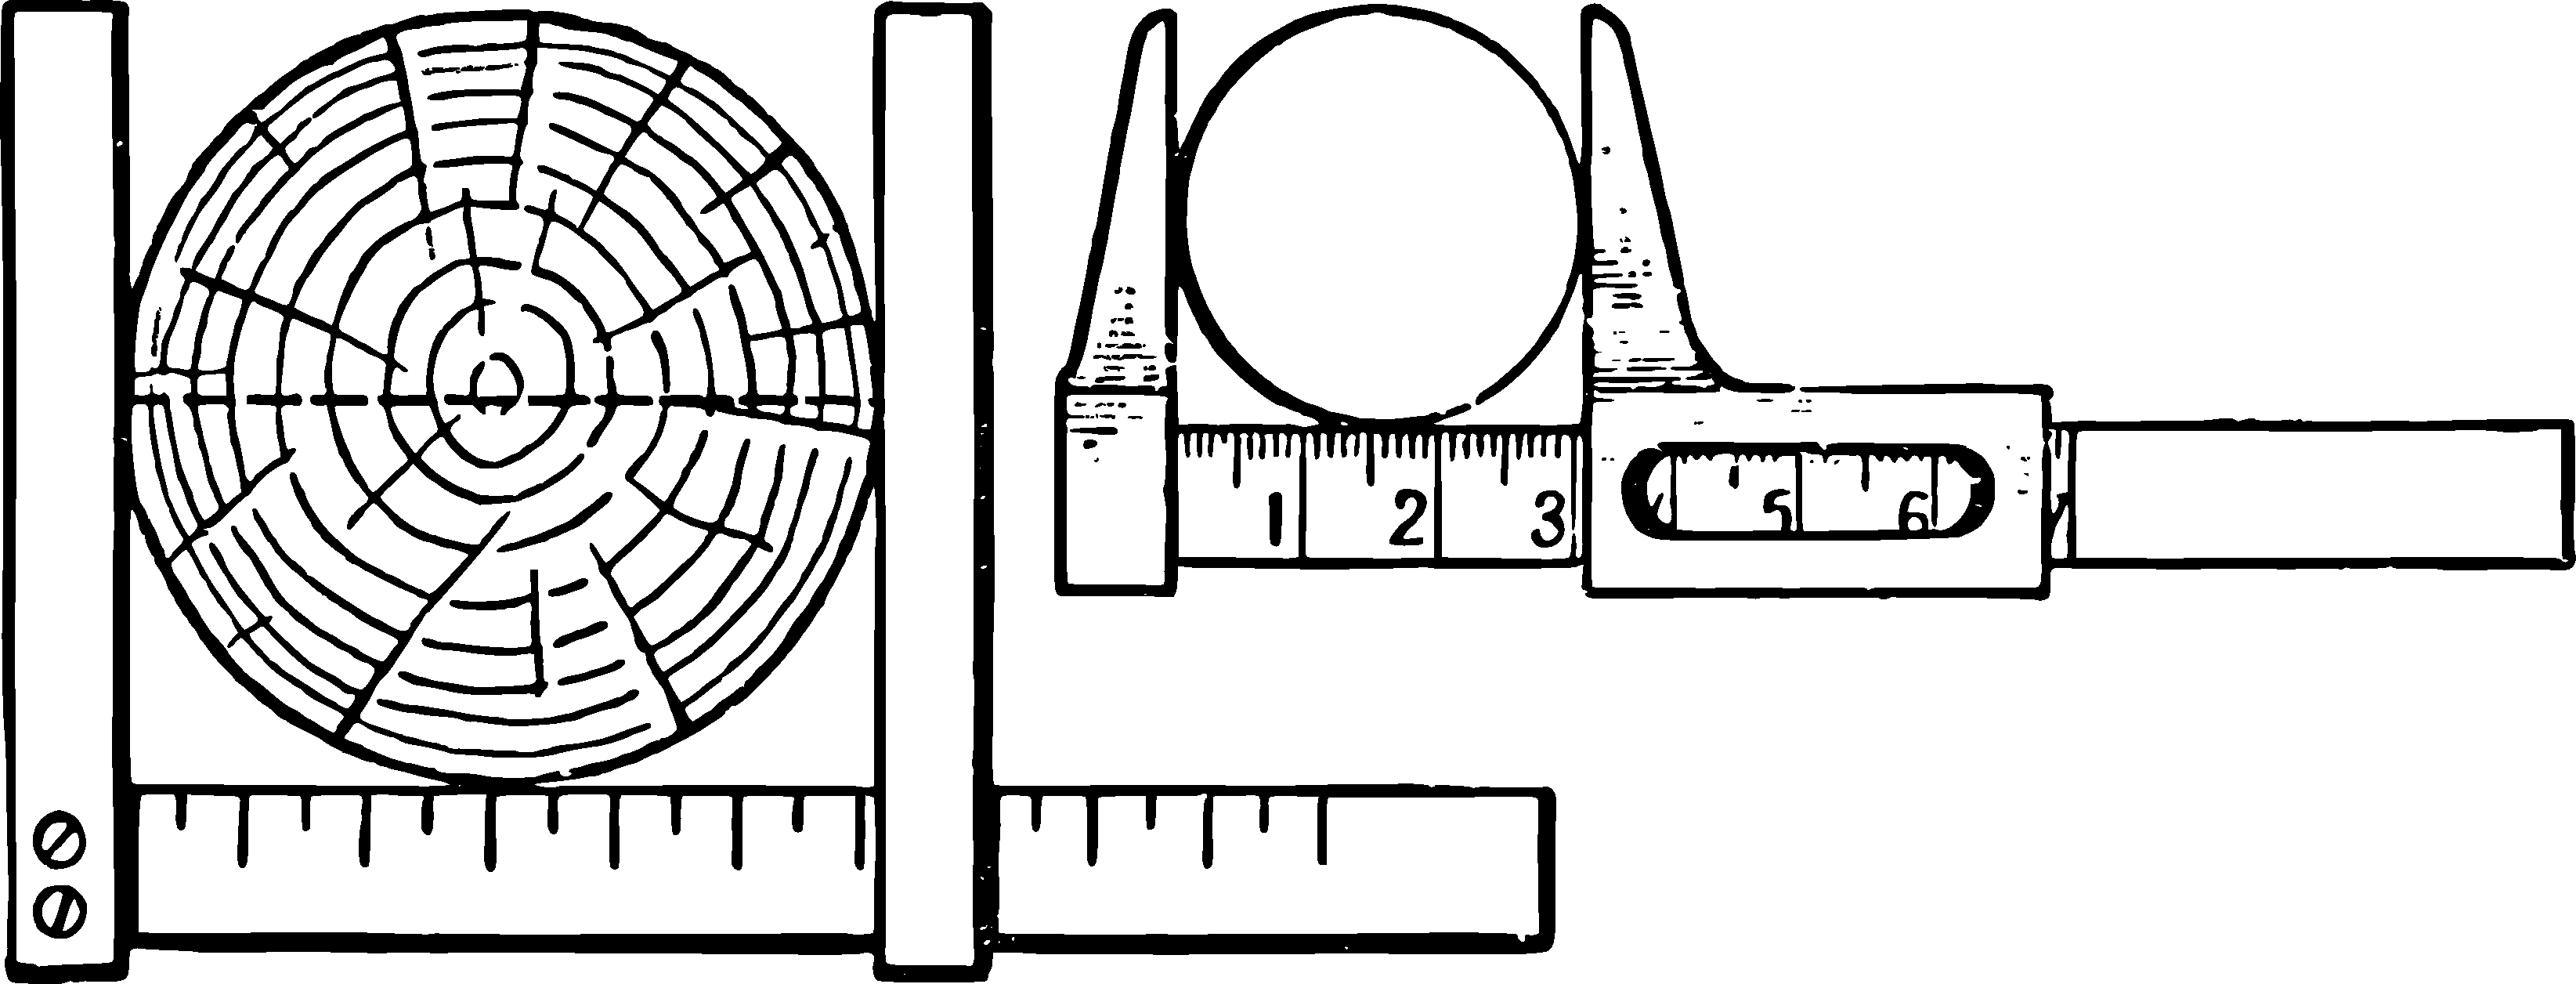
\includegraphics[width=0.9\textwidth]{figures/ch-01/fig-01-20.pdf}
\sidecaption{Measuring fork (left) and caliper (right).\label{fig-01-20}}
\end{figure}

However, all this is completely inapplicable to a tree at the root: if you are not going to climb it, then you can only measure the diameter of its lower part. In this case, to determine the volume, you will have to be satisfied with only a very approximate estimate, comforting yourself with the fact that professional foresters usually proceed in a similar way. They also use a table of so-called ``species numbers,'' i.e., numbers that show what proportion of the volume of the measured tree is compared to the volume of a cylinder of the same height and diameter, measured at the height of a grown man's chest, i.e., 130 cm (this height is the most convenient for measuring). 

\figr{fig-01-21} illustrates this clearly. Of course, ``species numbers'' vary for trees of different species and heights, as the shape of the trunk is variable. However, the fluctuations are not particularly great: for pine and fir trunks (grown in dense plantations), ``species numbers'' range from 0.45 to 0.51, i.e., are approximately half.

\begin{figure}[h!]
\centering
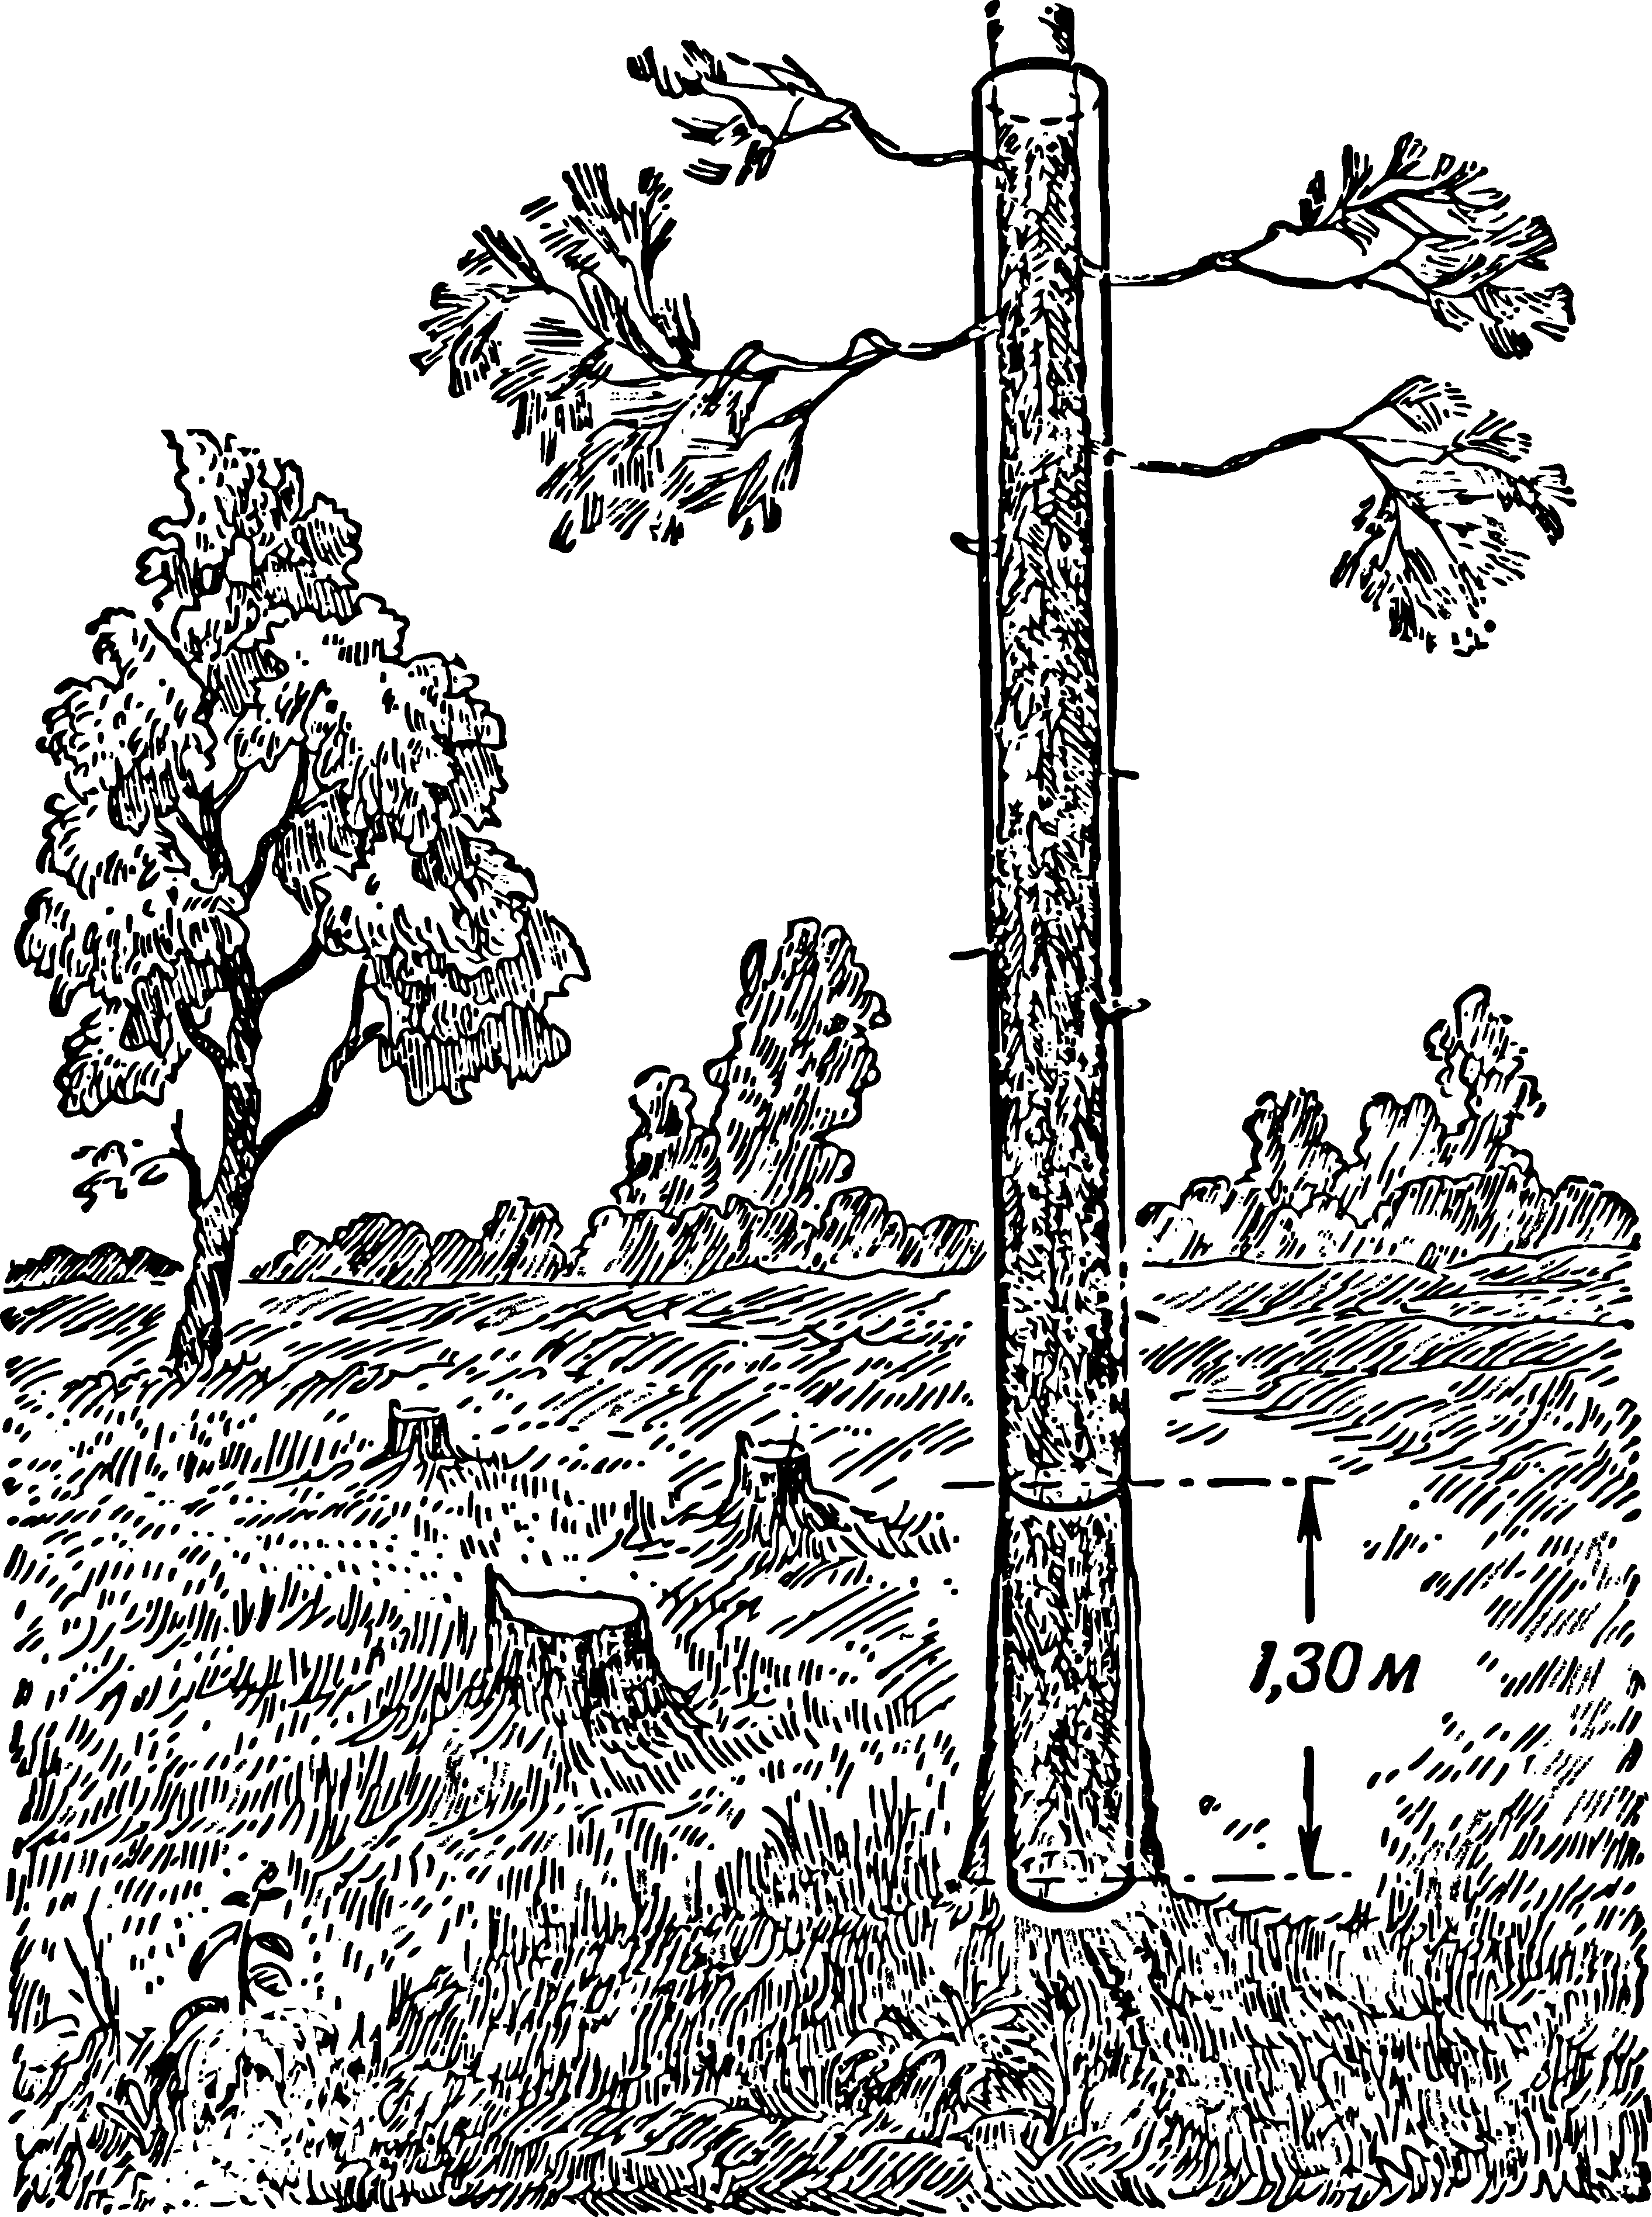
\includegraphics[width=0.8\textwidth]{figures/ch-01/fig-01-21.pdf}
\sidecaption[][-4cm]{What is a ``species number''?\label{fig-01-21}}
\end{figure}

Thus, without much error, it can be assumed that the volume of a coniferous tree at the root is half the volume of a cylinder of the same height with a diameter equal to the diameter of the tree at chest height.

This is, of course, only an approximate estimate, but it is not too far from the true result: up to 2\% in the overestimation direction and up to 10\% in the underestimation direction.\sidenote[][-1cm]{It must be remembered that ``species numbers'' refer only to trees that have grown in the forest, i.e. to tall and thin (smooth, without nodes); for free-standing branched trees, such general rules for calculating volume cannot be specified.}

From here, it is only one step towards estimating the weight of the tree at the root. For this, it is enough to know that 1 cubic meter of fresh pine or fir wood weighs about 600–700 kg. For example, suppose you are standing next to a fir tree, the height of which you have determined to be \SI{28}{\meter}, and the circumference of the trunk at chest height is \SI{120}{\centi\meter}. Then the area of the corresponding circle is \SI{1100}{\centi\meter\squared}, or \SI{0.11}{\meter\squared}, and the volume of the trunk is $1/2 \times 0.11 \times 28 = \SI{1.5}{\meter\cubed}$. Assuming that 1 cubic meter of fresh fir wood weighs on average \SI{650}{\kilo\gram}, we find that 1.0 cubic meter should weigh about a ton (\SI{1000}{\kilo\gram}).


\section{Leaf Geometry}
\label{sec-1.12}

\ques In the shadow of a silver poplar from its roots, a thicket has grown. Pick a leaf and notice how large it is compared to the leaves of the parent tree, especially those that grew in bright sunlight. The shaded leaves compensate for the lack of light with the size of their area, capturing sunlight rays. Understanding this is the task of botany. But the geometer can also have a say here: he can determine exactly how many times the area of the thicket leaf is larger than the area of the parent tree leaf.

How would you solve this problem?


\ans You can go two ways. First, determine the area of each leaf separately and find their ratio. The area of the leaf can be measured by covering it with transparent grid paper, each square of which corresponds, for example, to 4 square millimeters (a sheet of transparent grid paper used for this purpose is called a pallet). This is a perfectly correct but overly laborious method.\sidenote{However, this method has an advantage: using it, you can compare the areas of leaves with different shapes, which cannot be done according to the method described below.}

A shorter method is based on the fact that both leaves, different in size, still have the same or almost the same shape: in other words, they are geometrically similar figures. We know that the areas of such figures are related as the squares of their linear dimensions. Therefore, by determining how many times one leaf is longer or wider than the other, we can find the ratio of their areas simply by squaring this number. Let the thicket leaf be 15 cm long, and the leaf from the tree branch only 4 cm long; the ratio of their linear dimensions is 15/4, and therefore, in terms of area, one is larger than the other by 225/16 times, or about 14. Rounding off (since full accuracy cannot be achieved here), we can say that the thicket leaf is approximately 15 times larger than the tree leaf in terms of area.

Let us consider another example.
%\clearpage

\ques At a dandelion grown in shade, a leaf is 31 cm long. At another specimen grown in sunlight, the leaf blade is only 3.3 cm long. Approximately how many times is the area of the first leaf larger than the area of the second?



\ans We proceed as before. The ratio of the areas is
\begin{equation*}%
\frac{31^{2}}{3.3^{2}} = \frac{960}{10.9} = 87;
\end{equation*}
so one leaf is approximately 90 times larger than the other in terms of area.

\begin{marginfigure}[-3.5cm]%[h!]
\centering
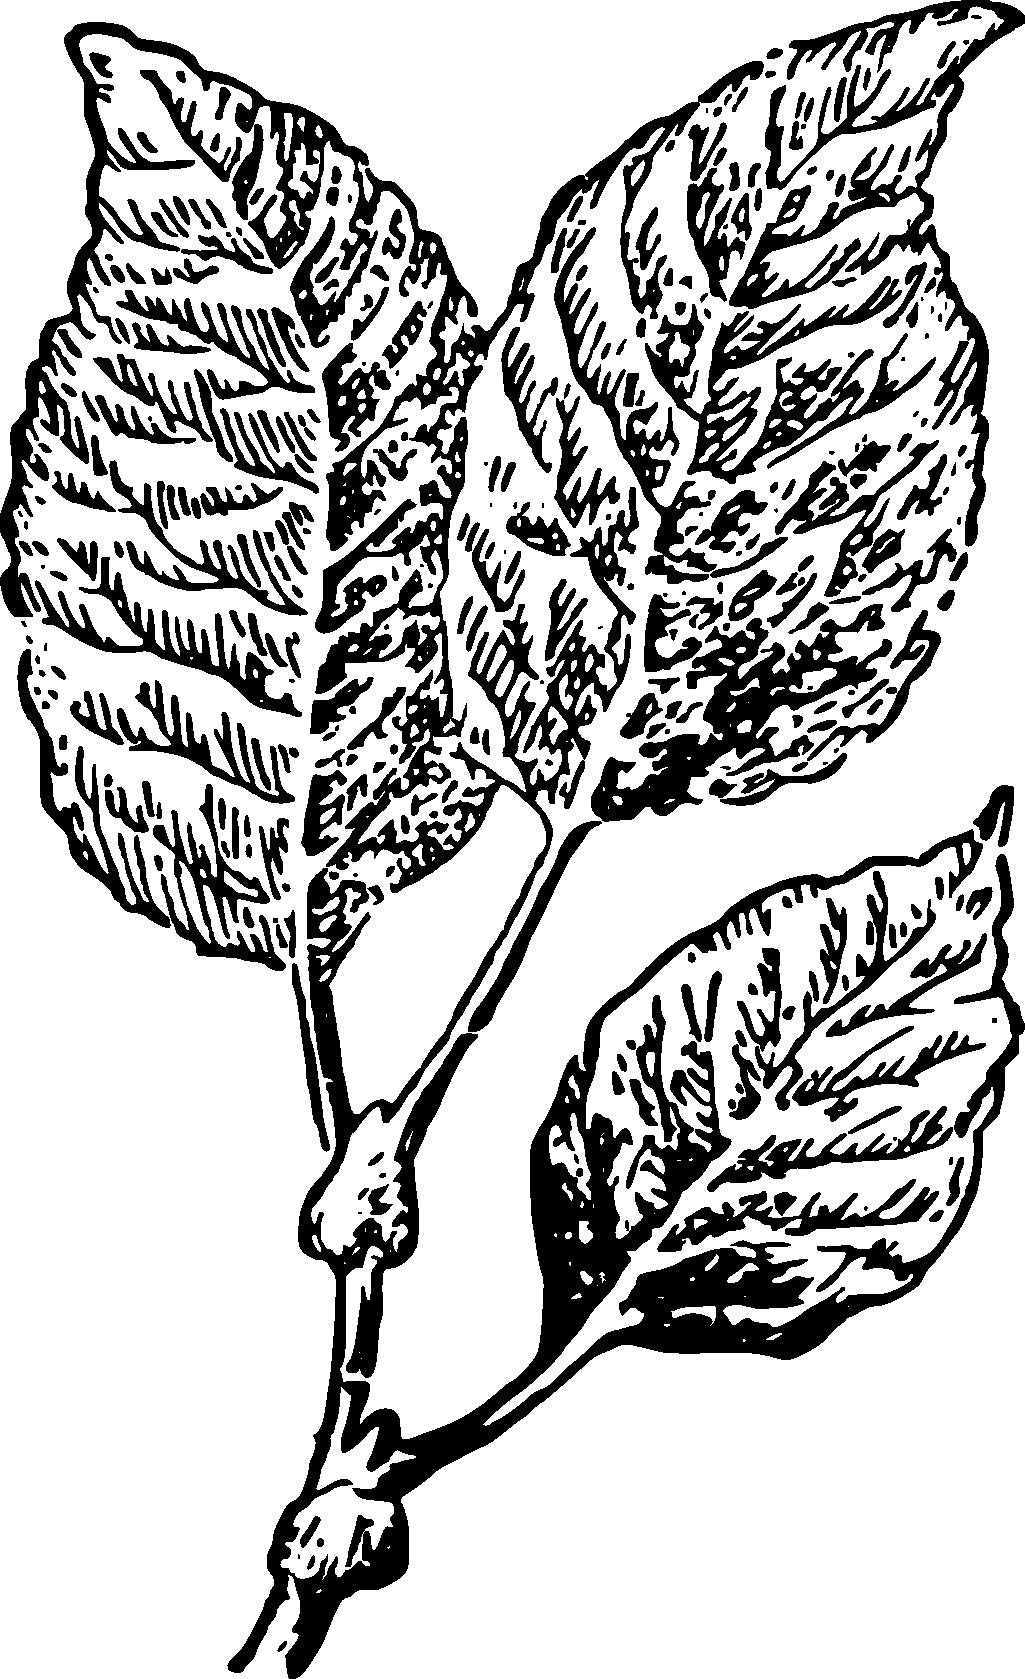
\includegraphics[width=0.9\textwidth]{figures/ch-01/fig-01-22.pdf}
\sidecaption{Determine the ratio of the areas of these leaves.\label{fig-01-22}}
\end{marginfigure}


It is easy to find in the forest many pairs of leaves of the same shape but different sizes, thus providing interesting material for geometric problems on the ratio of areas of similar figures. It always seems strange to an unaccustomed eye that a relatively small difference in the length and width of leaves results in a noticeable difference in their areas. For example, if two leaves, geometrically similar in shape, differ in length by 20\%, then the ratio of their areas is 
\begin{equation*}%
1.2^{2} \approx 1.4, 
\end{equation*}
meaning the difference is 40\%. And with a difference in width of 40\%, One leaf exceeds the other in area by 
\begin{equation*}%
1.4^{2} \approx 2, 
\end{equation*}
or nearly twice.

\ques  We invite the reader to determine the ratio of the areas of the leaves depicted in \figr{fig-01-22} and \figr{fig-01-23}.

\begin{marginfigure}[-4.5cm]%[h!]
\centering
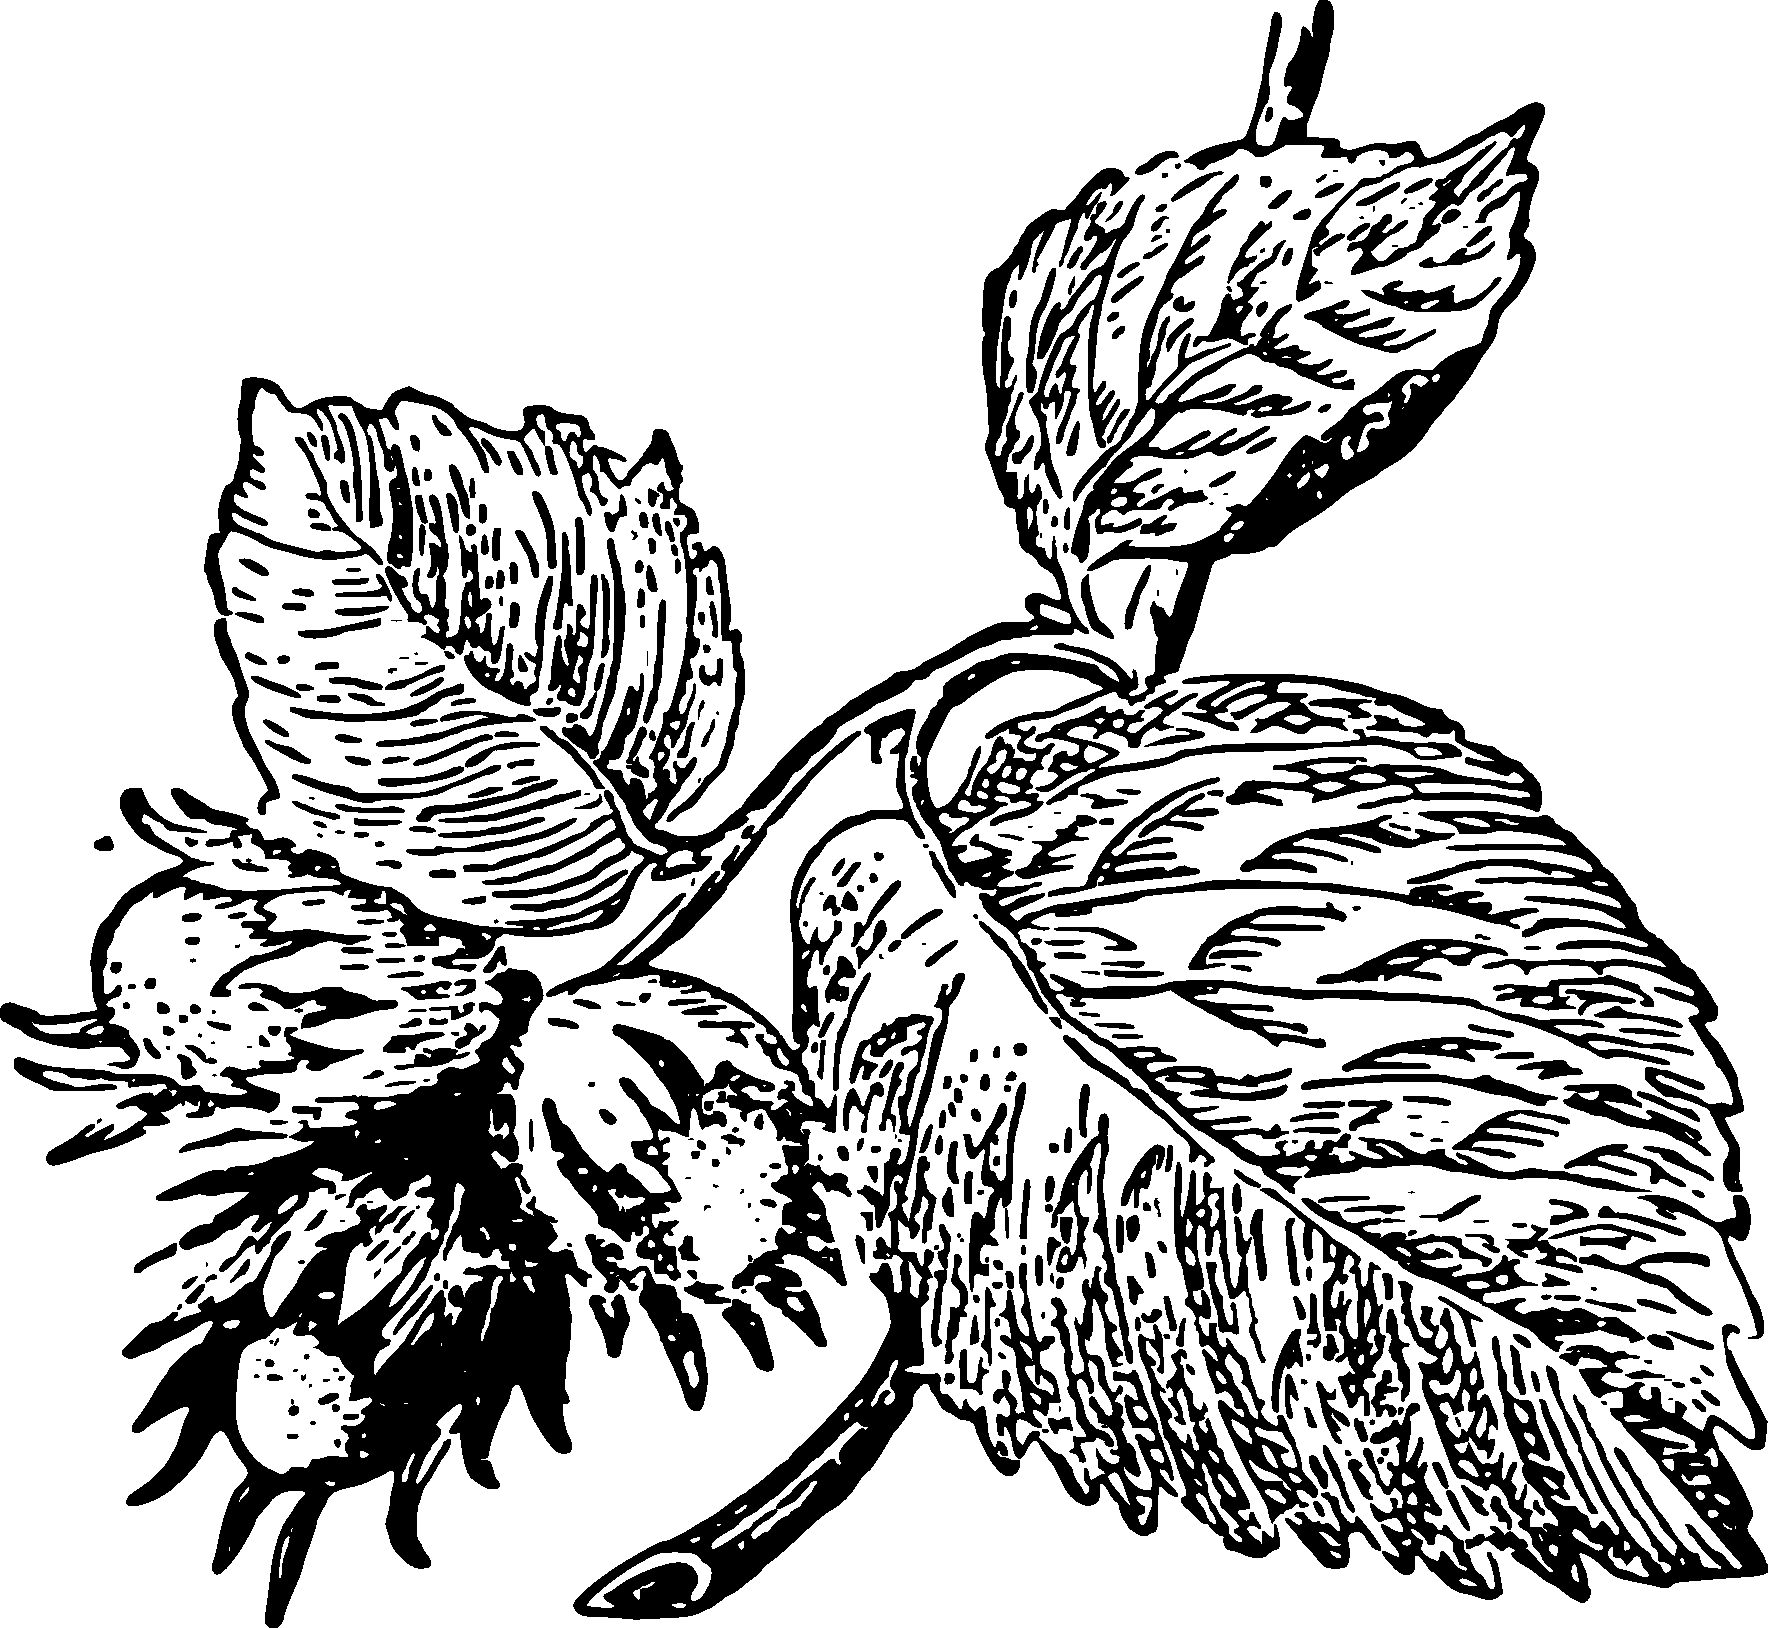
\includegraphics[width=0.9\textwidth]{figures/ch-01/fig-01-23.pdf}
\sidecaption{Determine the ratio of the areas of these leaves.\label{fig-01-23}}
\end{marginfigure}


%\ques \textsf{\small\color{Salmon} We invite the reader to determine the ratio of the areas of the leaves depicted in \figr{fig-01-22}and \figr{fig-01-23}.}

\section{Six-legged heroes}
\label{sec-1.14}

Amazing creatures, ants! Swiftly climbing up stems with a burden much heavier than their tiny size (\figr{fig-01-24}), ants present an intriguing puzzle to observant individuals: where does the insect derive the strength to effortlessly carry a load ten times its own weight? Indeed, a human might struggle to climb stairs while carrying, for instance, a piano (\figr{fig-01-24}), with the weight ratio of the load to the body being roughly similar to that of an ant. Thus, it seems that the ant is relatively stronger than a human!

But is it really so?

Without geometry, this cannot be understood. Let's listen to what the expert (Professor A.F. Brandt) has to say, primarily about the strength of muscles, and then about the current question regarding the comparison of forces between the insect and the human: ``A muscle resembles a resilient cord; however, its contraction is based not on elasticity, but on other reasons, and is normally manifested under the influence of nervous excitation, as demonstrated in physiological experiments involving the application of electric current to the corresponding nerve or directly to the muscle.''

``These experiments are easily conducted on muscles excised from a freshly killed frog, as the muscles of cold-blooded animals retain their vital properties for a long time even outside the organism, even at ordinary temperatures. The experiment is very simple. The main calf muscle, which extends the hind leg, is excised together with a piece of the femur bone from which it originates, and together with the terminal tendon. This muscle is found to be the most convenient due to its size, shape, and ease of preparation. A hook is passed through the tendon, and a weight is attached to it.'' 

\begin{marginfigure}[-3cm]%[h!]
\centering
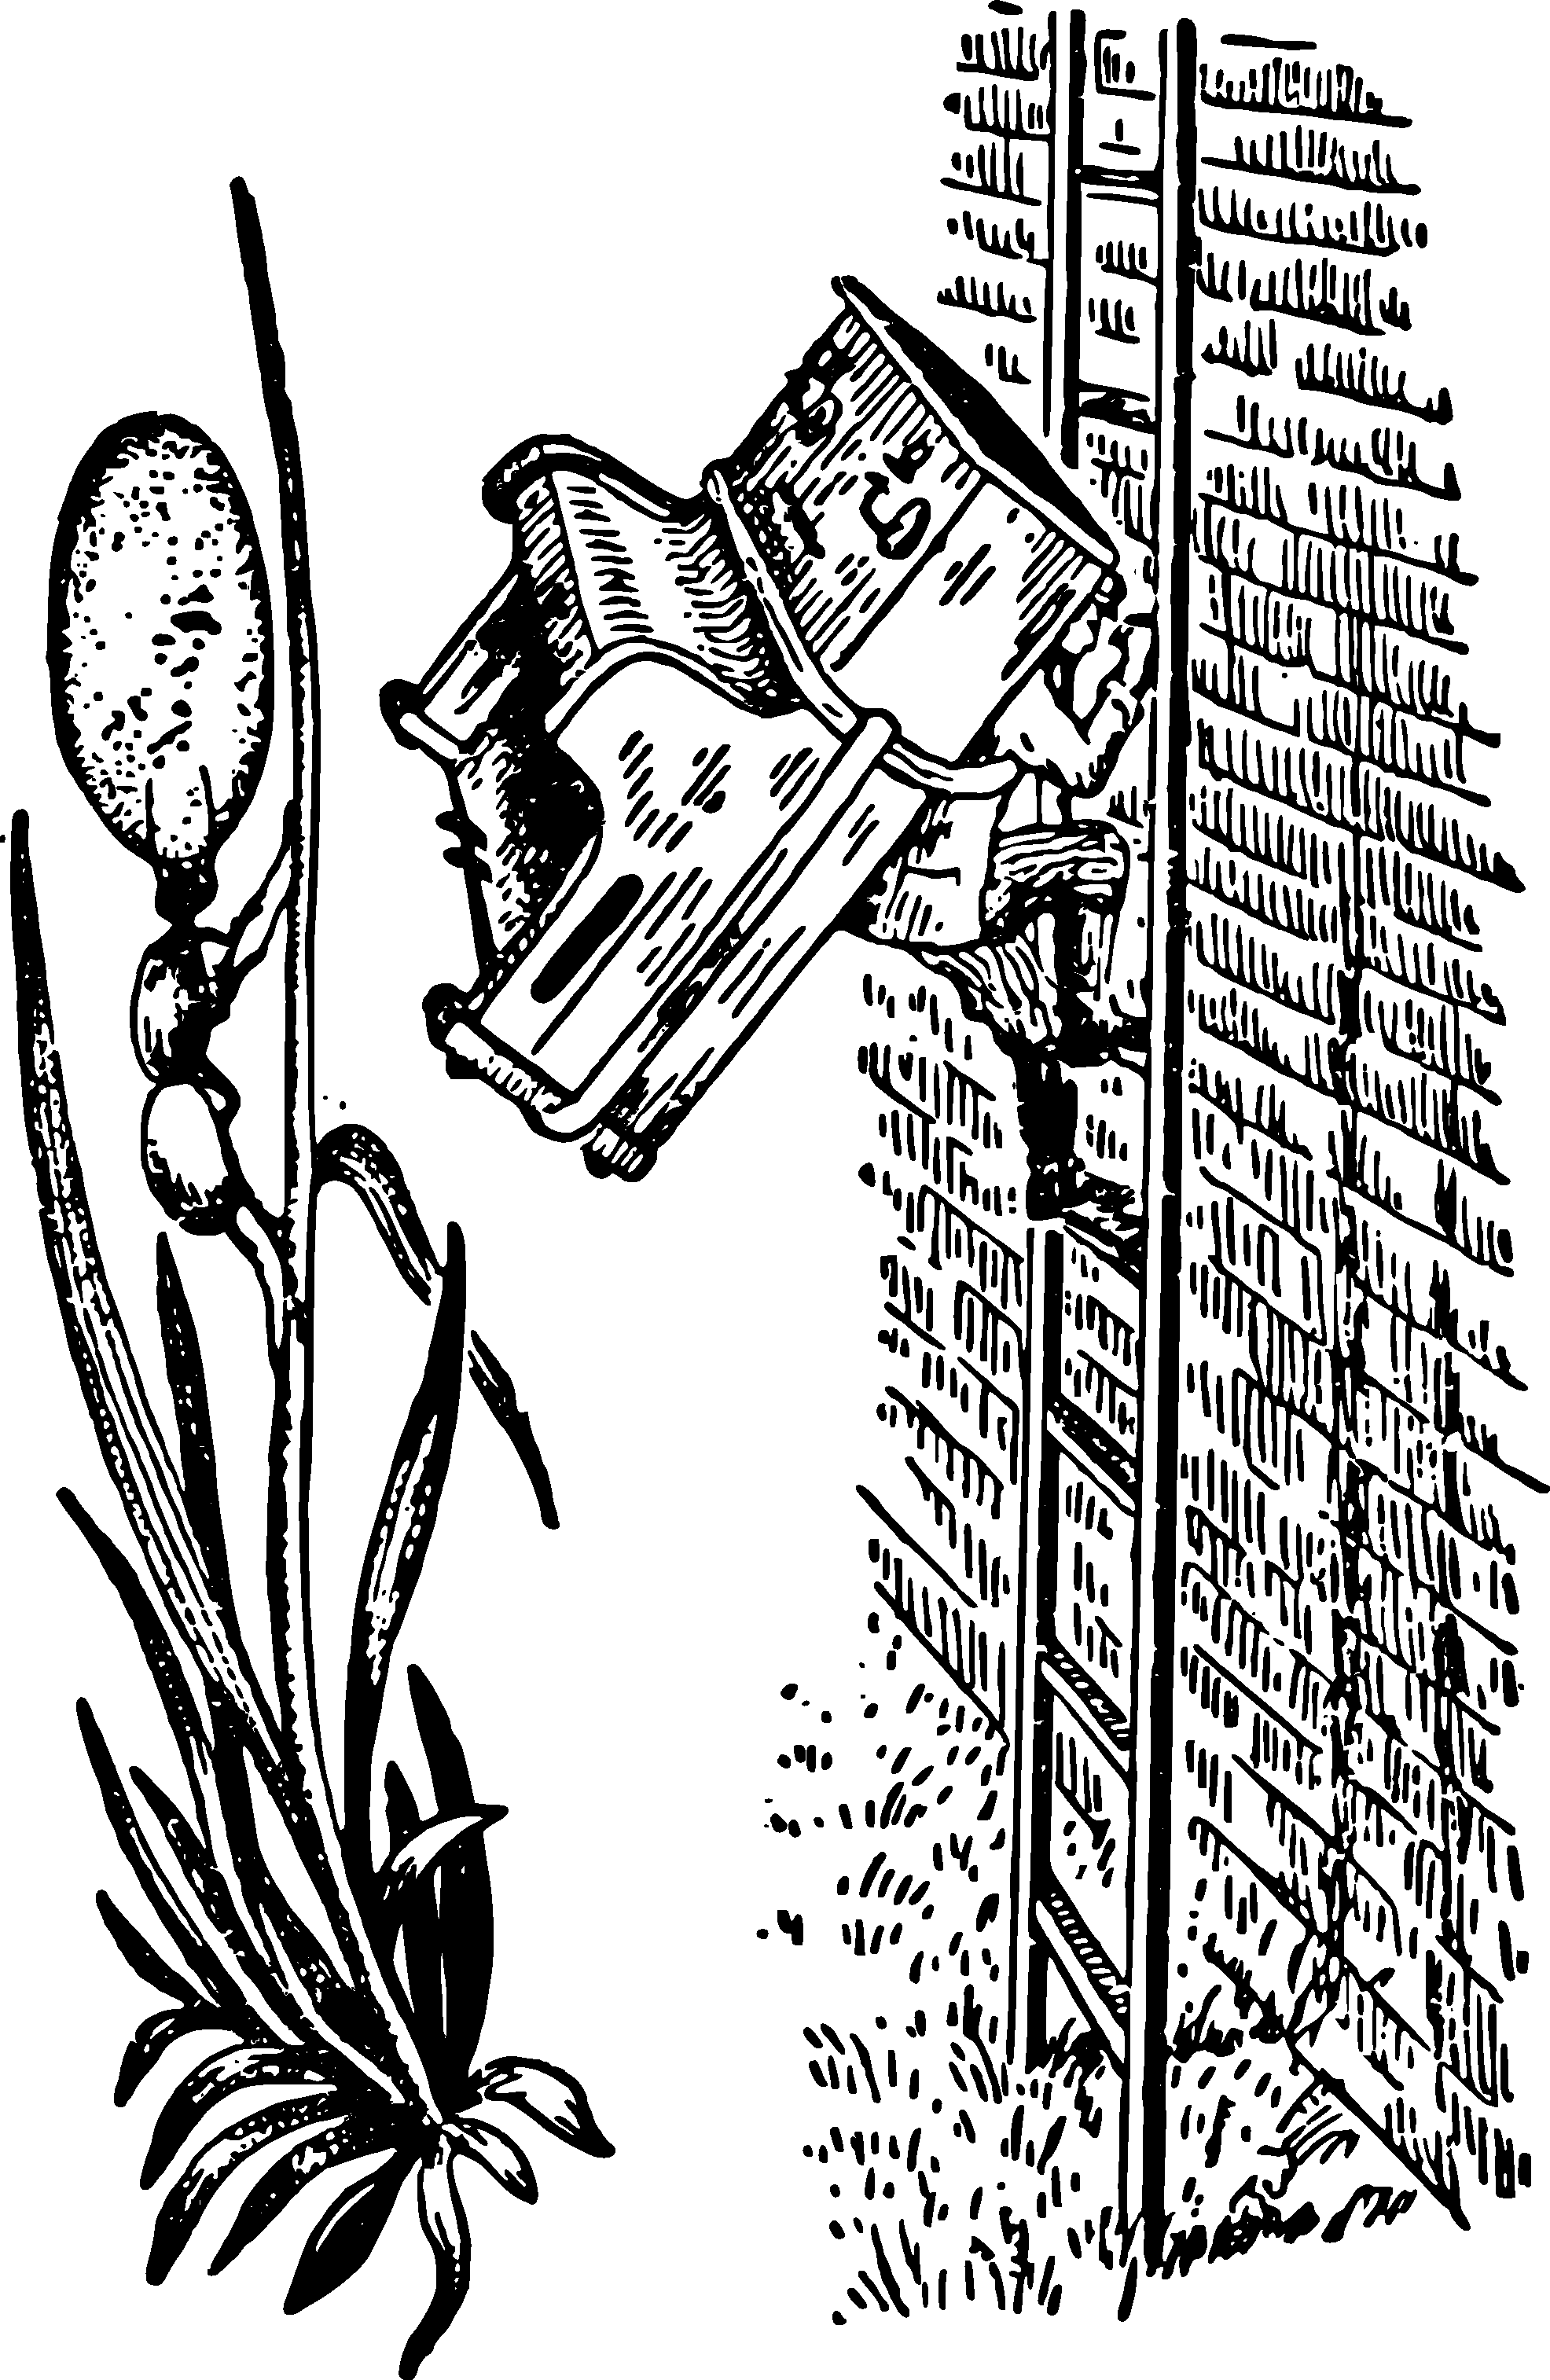
\includegraphics[width=\textwidth]{figures/ch-01/fig-01-24.pdf}
\sidecaption{The six-legged hero.\label{fig-01-24}}
\end{marginfigure}


``If wires from a galvanic element are touched to such a muscle, it instantly contracts, shortens, and lifts the load. By gradually adding additional weights, the maximum lifting capacity of the muscle can be easily determined. Now, if we bind together in length two, three, or four identical muscles and stimulate them simultaneously, we will not achieve greater lifting force; the load will only be lifted to a greater height, corresponding to the sum of the contractions of individual muscles. However, if we bundle two, three, or four muscles together, the entire system will lift a weight many times greater when stimulated. The same result, obviously, would be obtained if the muscles were fused together. Thus, we conclude that the lifting force of muscles depends not on their length or total mass, but only on their thickness, i.e., \emph{cross-sectional area}.''

``After this digression, let's turn to the comparison of similarly structured, geometrically similar, but differently sized animals. Let's imagine two animals: the original and one that has been doubled in size in all linear dimensions. In the second animal, the volume and weight of the entire body, as well as each of its organs, will be eight times greater; however, all corresponding planar dimensions, including the cross-sectional area of muscles, will be only four times greater. It turns out that as the animal grows to twice the length and eight times the weight, its muscular strength increases only fourfold, i.e., the animal becomes relatively weaker. Based on this reasoning, an animal that is three times longer (with cross-sectional areas three times larger and a weight 27 times greater) would be relatively three times weaker, and one that is four times longer would be four times weaker, and so on.''

``The law of unequal growth in volume and weight of the animal, and thus of muscular strength, explains why insects -- as observed in ants, predatory wasps, and others -- can carry loads 30 to 40 times their own weight, whereas a human can typically carry excluding gymnasts and porters -- only about 9/10 times their own weight, -- and a horse, which we view as a magnificent living work machine, even less, namely, only about 7/10 of its own weight.''\sidenote{For more details, see \emph{Fun with Physics} by Ya. I. Perelman, Chapter X \emph{Mechanics in the Living World}.}

After these explanations, we will look at the feats of that ant-giant with different eyes, about whom I.A. Krylov mockingly wrote:
\begin{quote}
\emph{Some ant had extraordinary strength,\\
 Such as was unheard of even in ancient times; \\
 He even (says his faithful historian)\\
 Could lift two barley grains.}
\end{quote} 


\begin{center}

\includegraphics[width=0.3\textwidth]{figures/ch-01/fig-ch-01-tail.pdf}
\end{center}



















% !TEX root = perelman-geometry.tex
%!TEX TS-program = pdflatex
%!TEX encoding = UTF-8 Unicode

\setchapterpreamble[o]{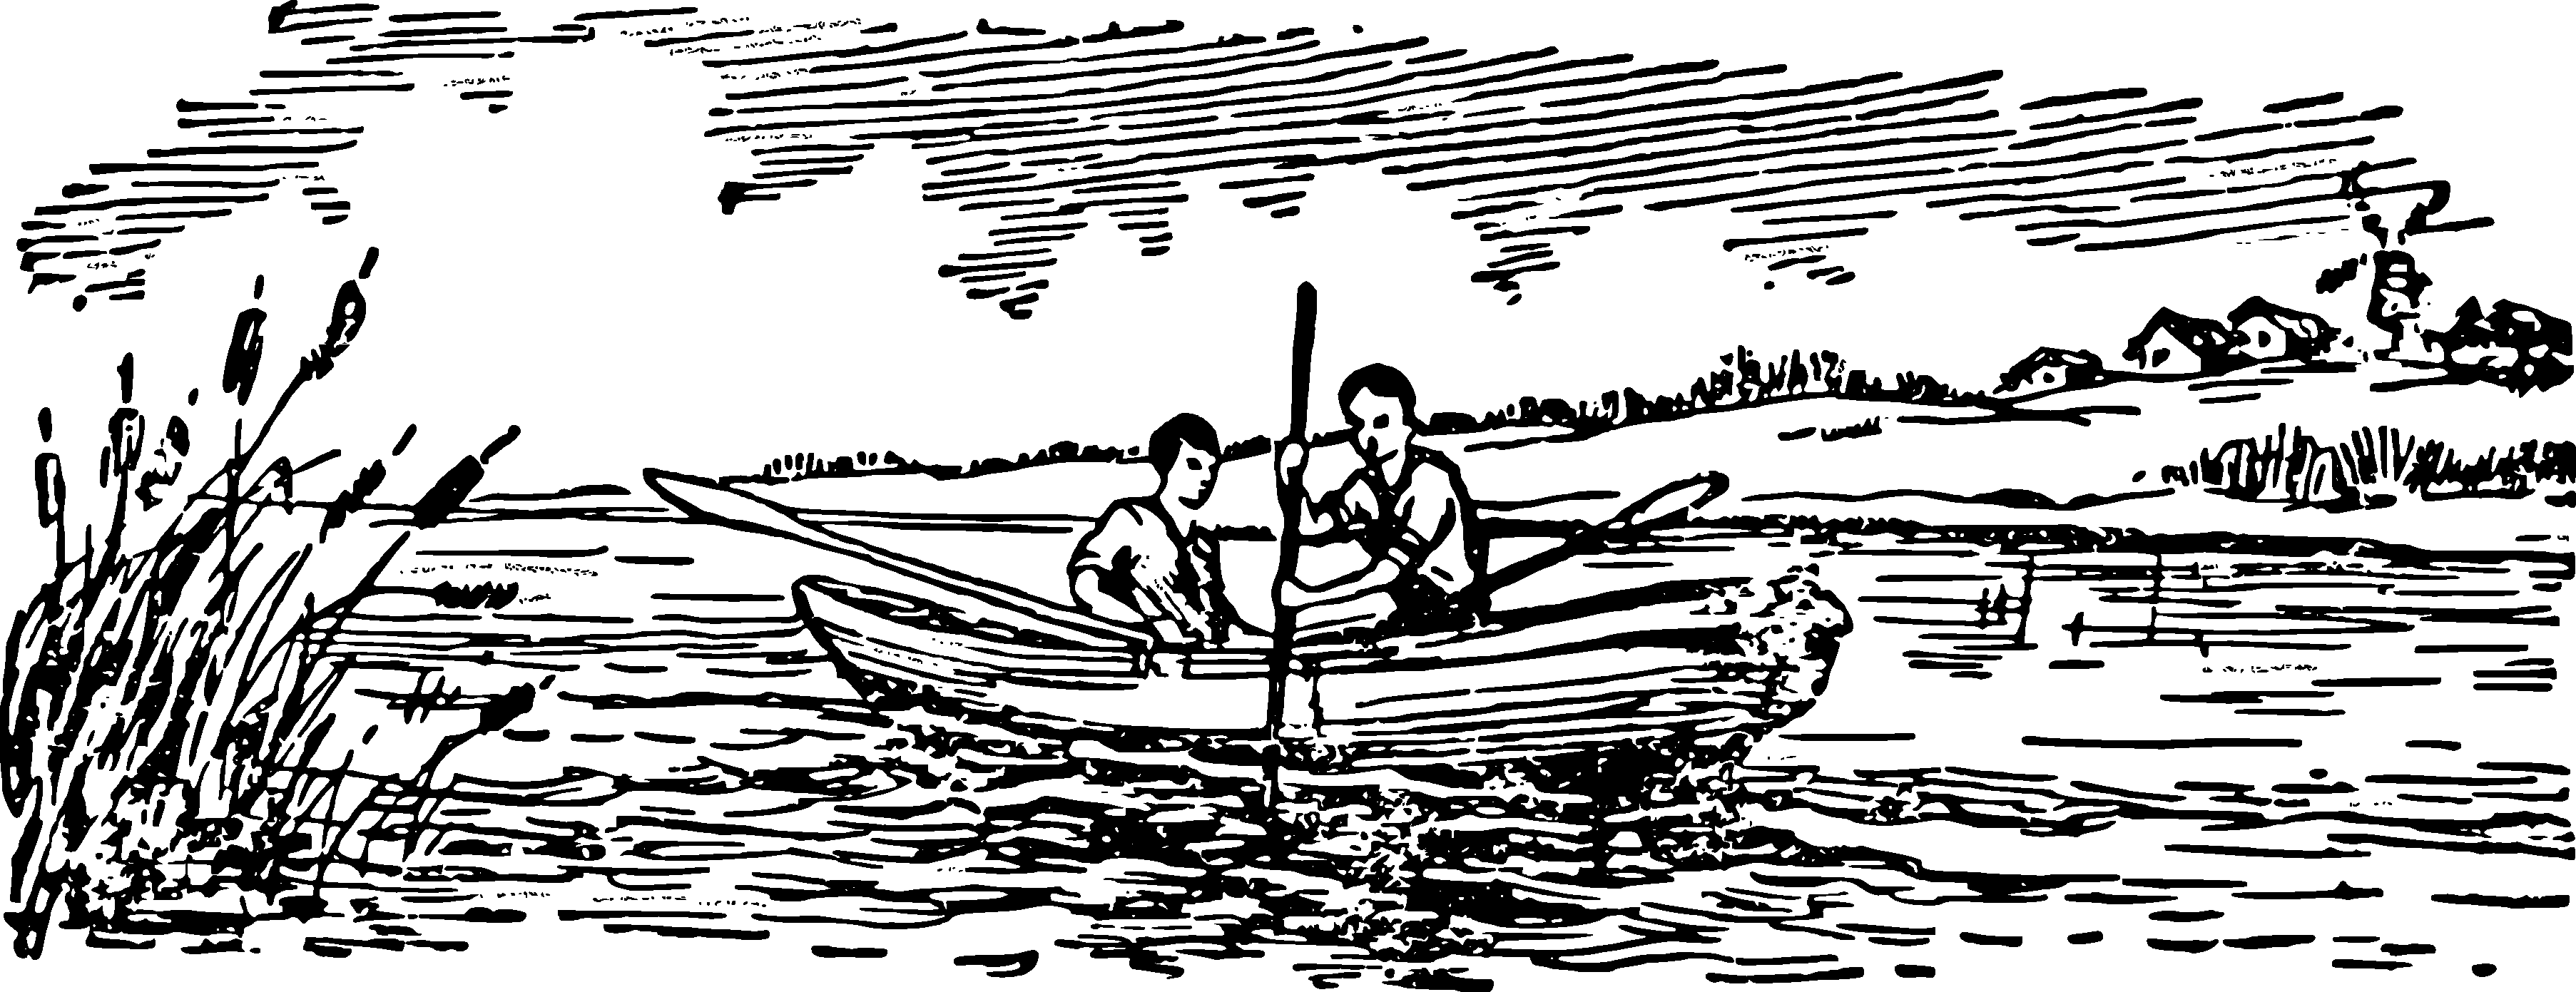
\includegraphics[width=1.2\textwidth]{figures/ch-02/fig-ch-02-head.pdf}\bigskip}

\chapter{Geometry By The River}
\label{ch-02}

\section{Measuring the width of the river}
\label{sec-2.1}
When crossing a river, measuring its width is just as easy for those who know geometry, how to determine the height of a tree, without climbing to the top. The inaccessible distance is measured the same techniques that we used to measure the inaccessible height. In both cases, the definition of the desired distance is replaced an example of another distance that is easily measurable directly.

Of the many ways to solve this problem, let's look at some of the simplest ones.

\begin{figure}[h!]
\centering
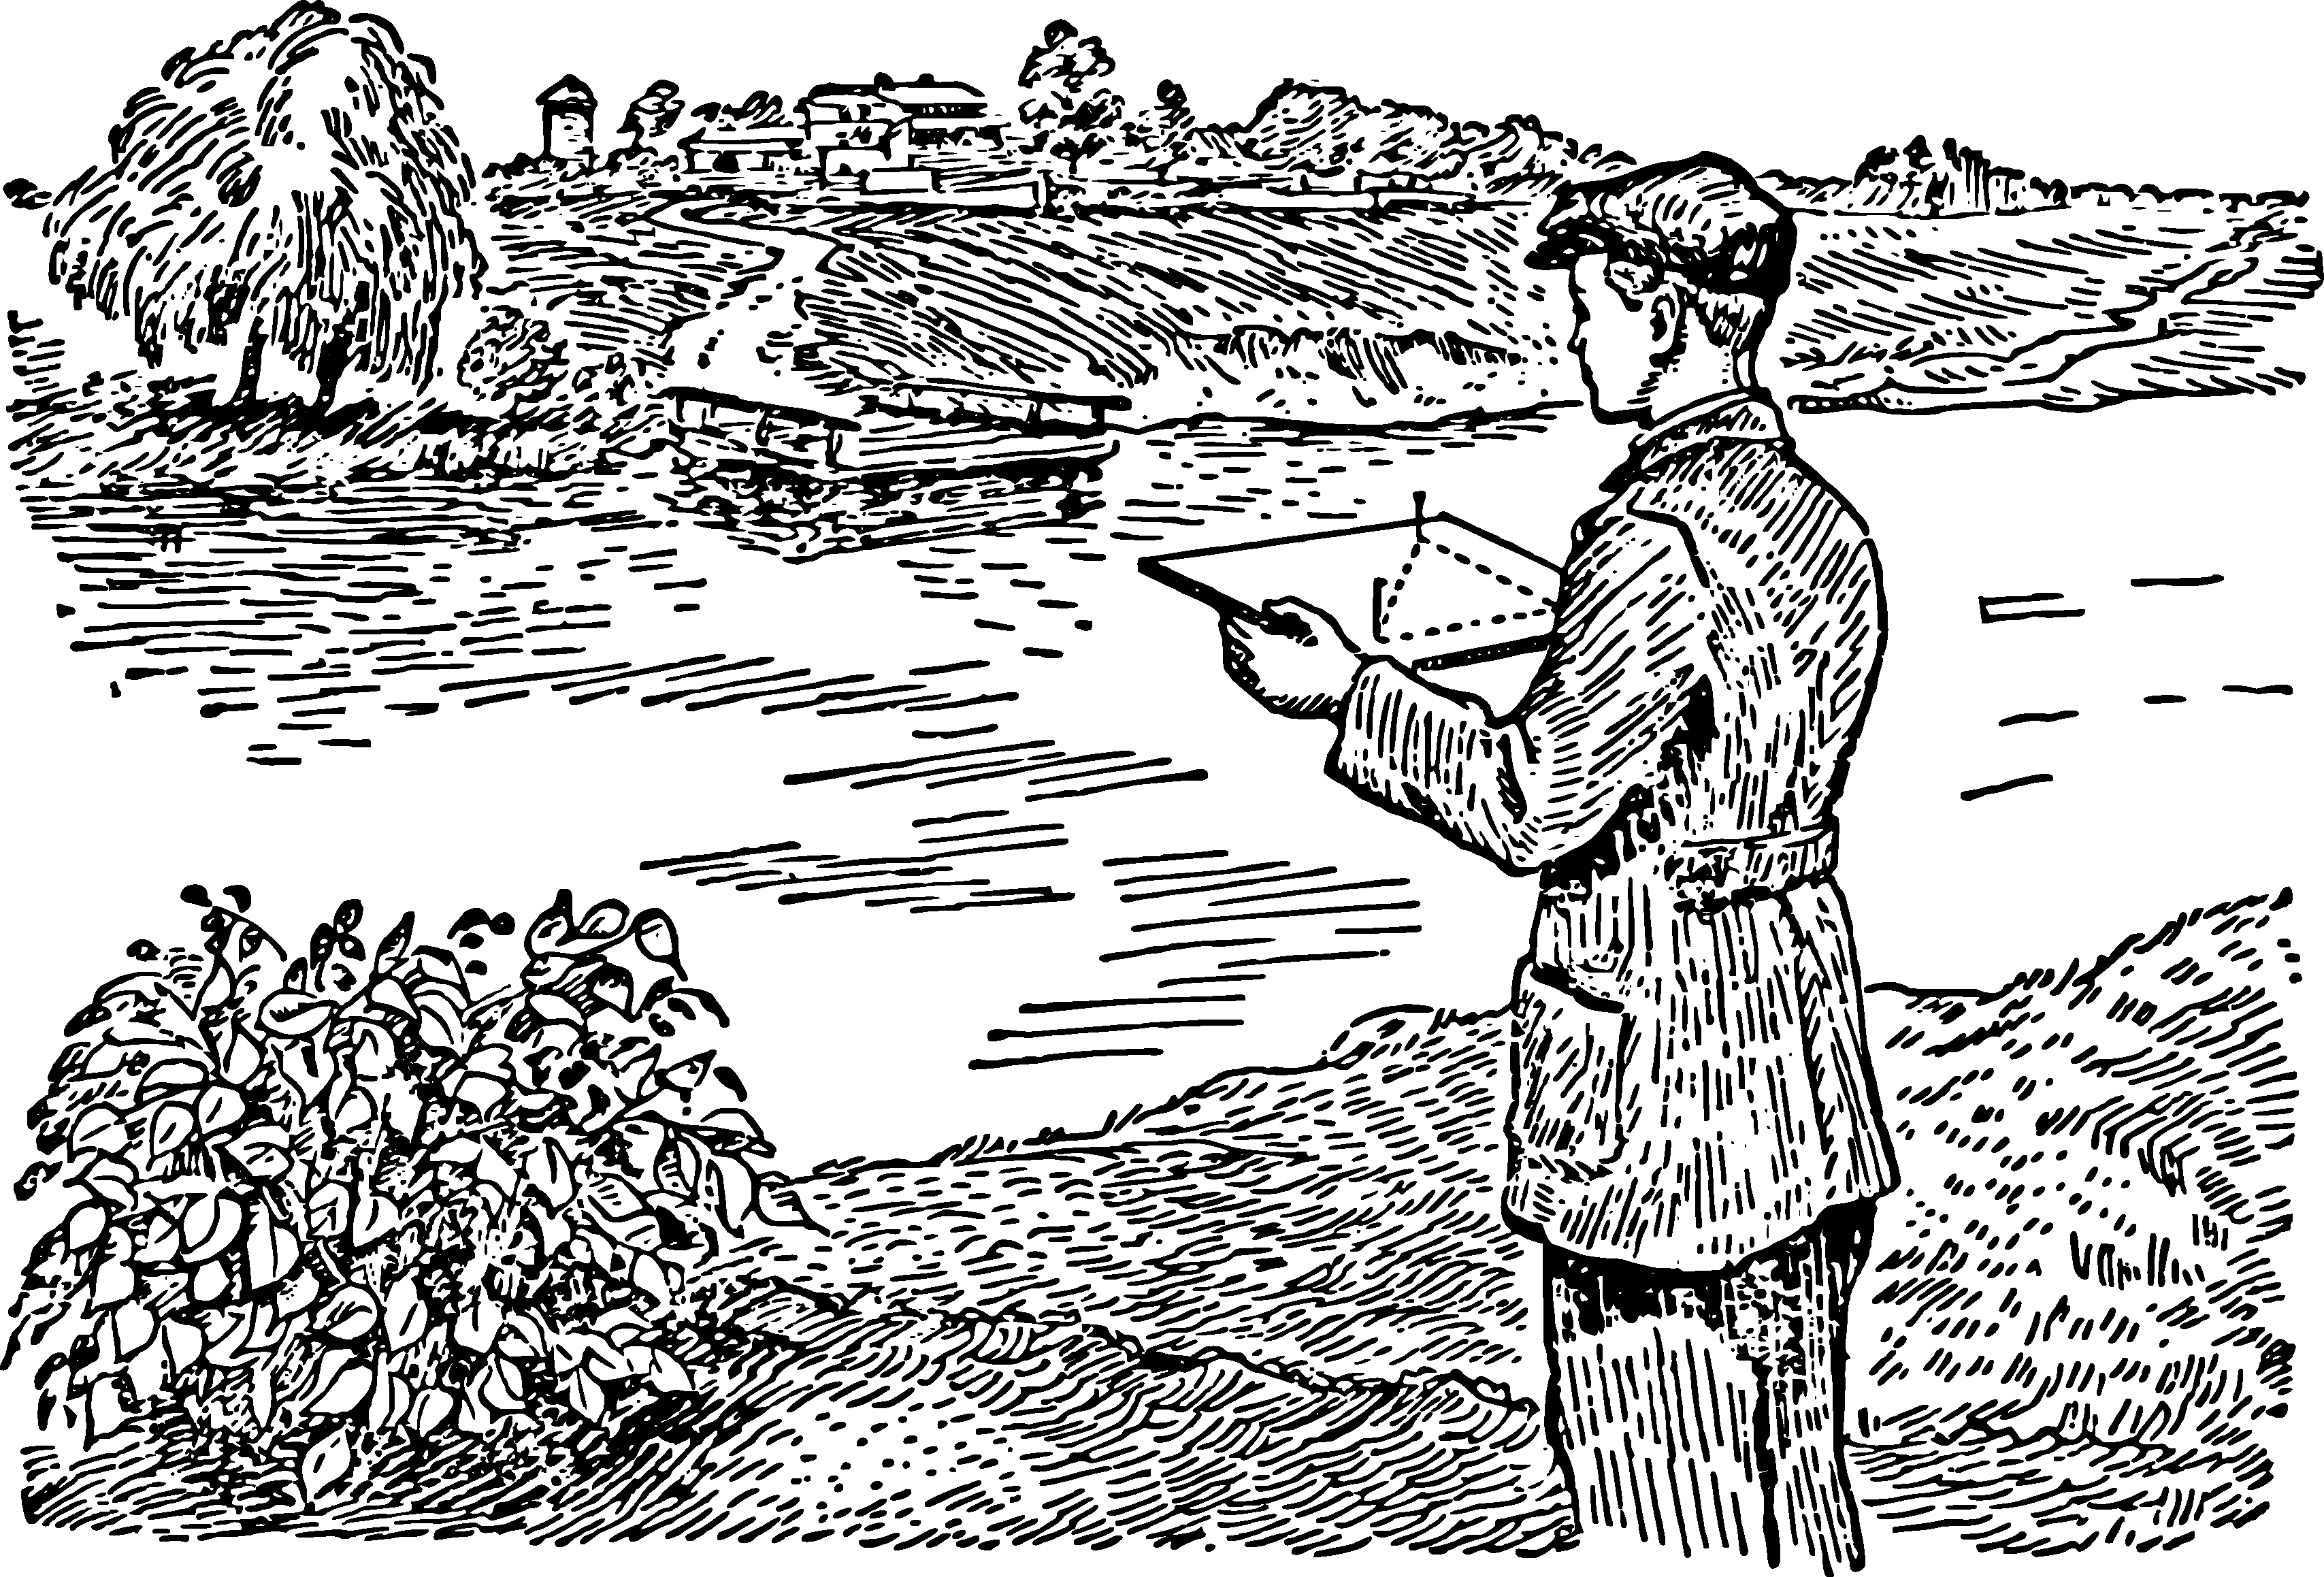
\includegraphics[width=0.9\textwidth]{figures/ch-02/fig-025.pdf}
\sidecaption{Measuring the width of the river with a pin device.\label{fig-025}}
\end{figure}

\begin{enumerate}
\item The first method requires the familiar ``device'' with three pins at the vertices of an isosceles right triangle (\figr{fig-025}). 
Let's say we need to determine the width of river $AB$ (\figr{fig-026}), standing on the bank where point $B$ is, without crossing to the opposite bank. Standing somewhere at point $C$, hold the pin device close to your eye so that, looking with one eye along the two pins, you see both covering points $B$ and $A$. It's clear that when you manage this, you will be exactly on the extension of line $AB$. 

\begin{marginfigure}[-1.5cm]%[h!]
\centering
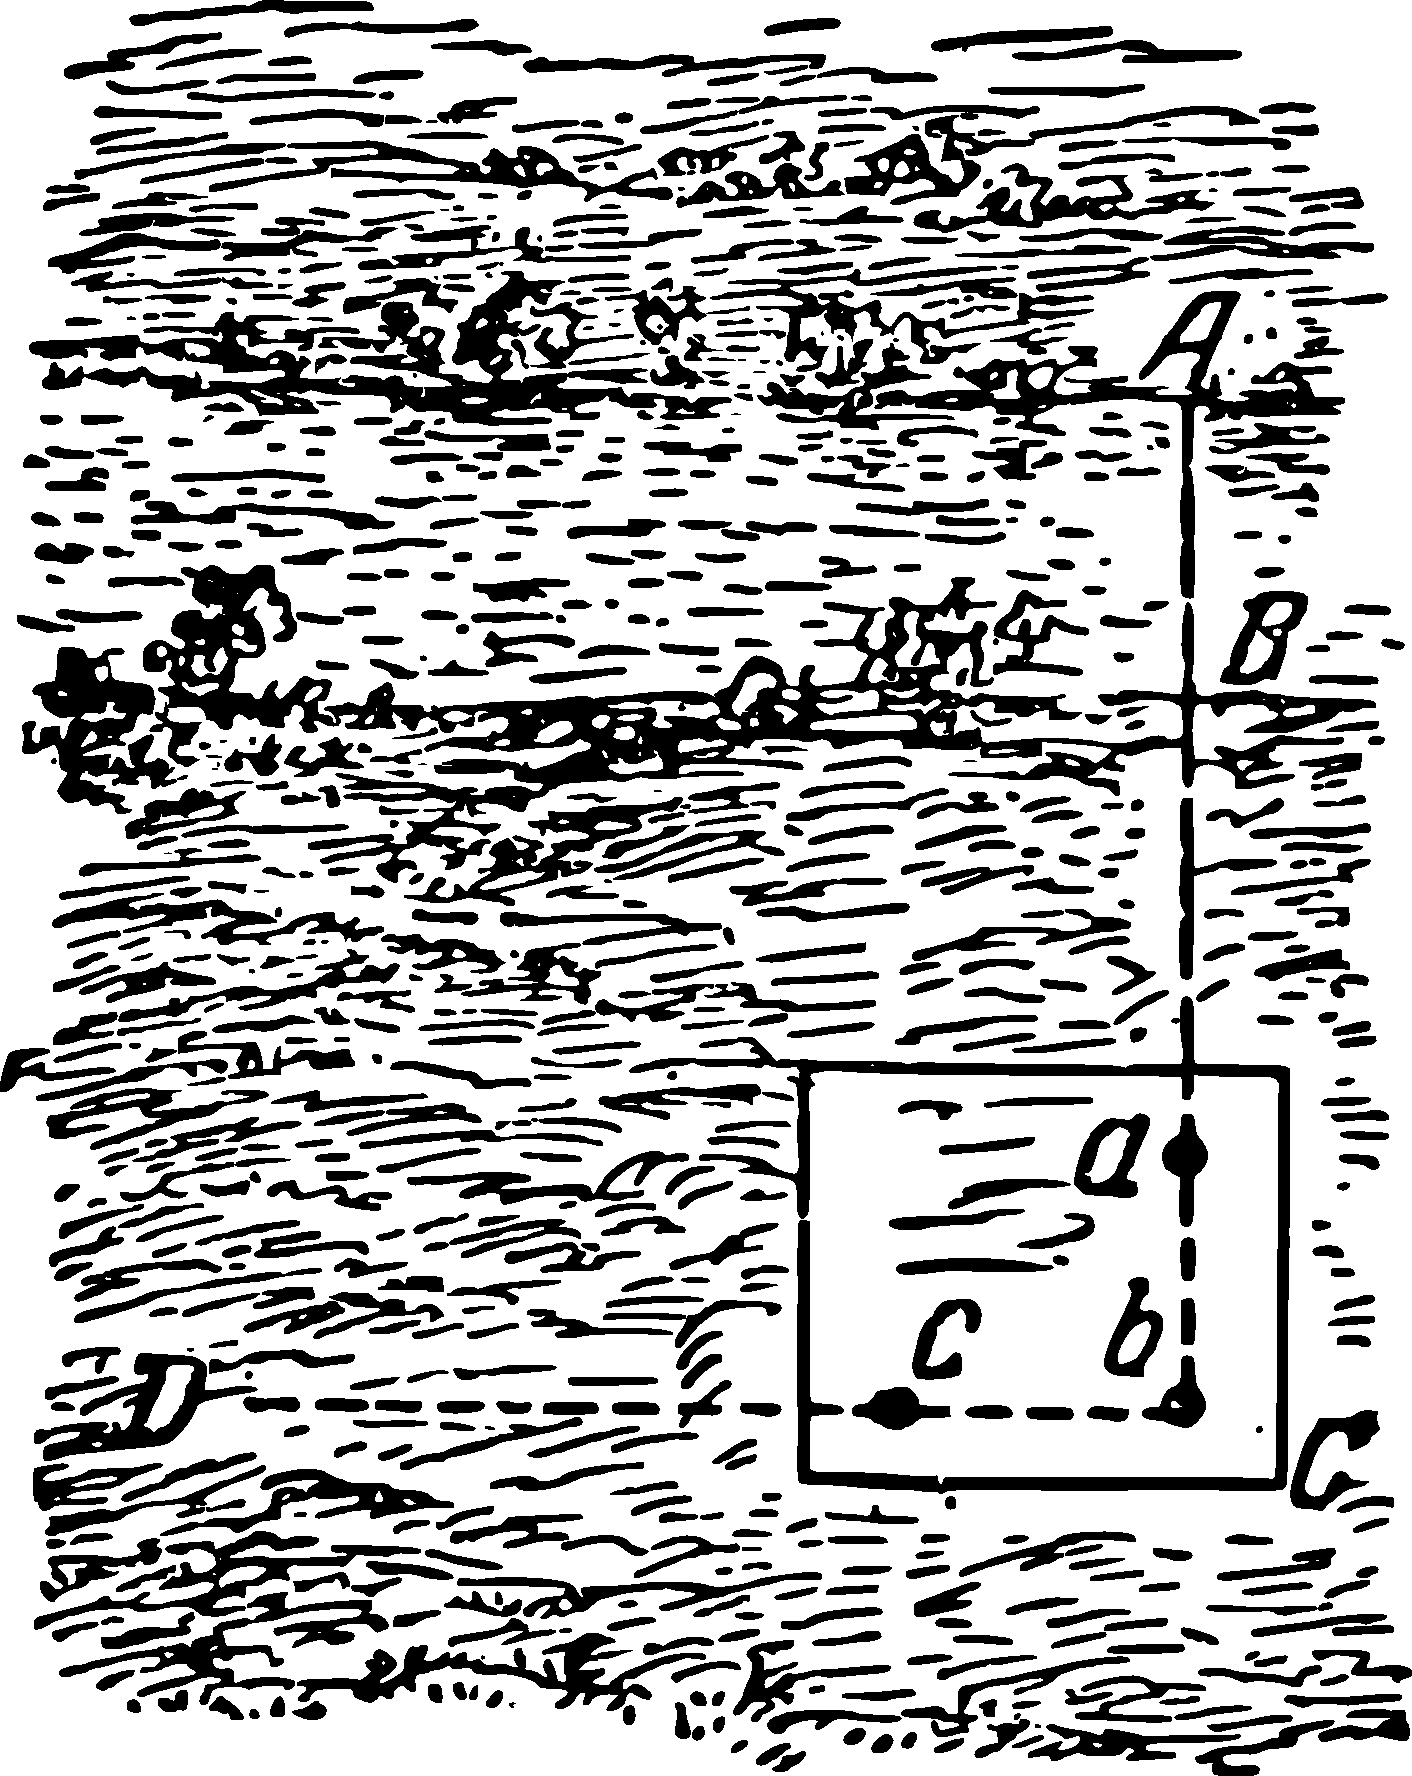
\includegraphics[width=\textwidth]{figures/ch-02/fig-026.pdf}
\sidecaption{First position of the pin device.\label{fig-026}}
\end{marginfigure}
\begin{marginfigure}[5cm]%[h!]
\centering
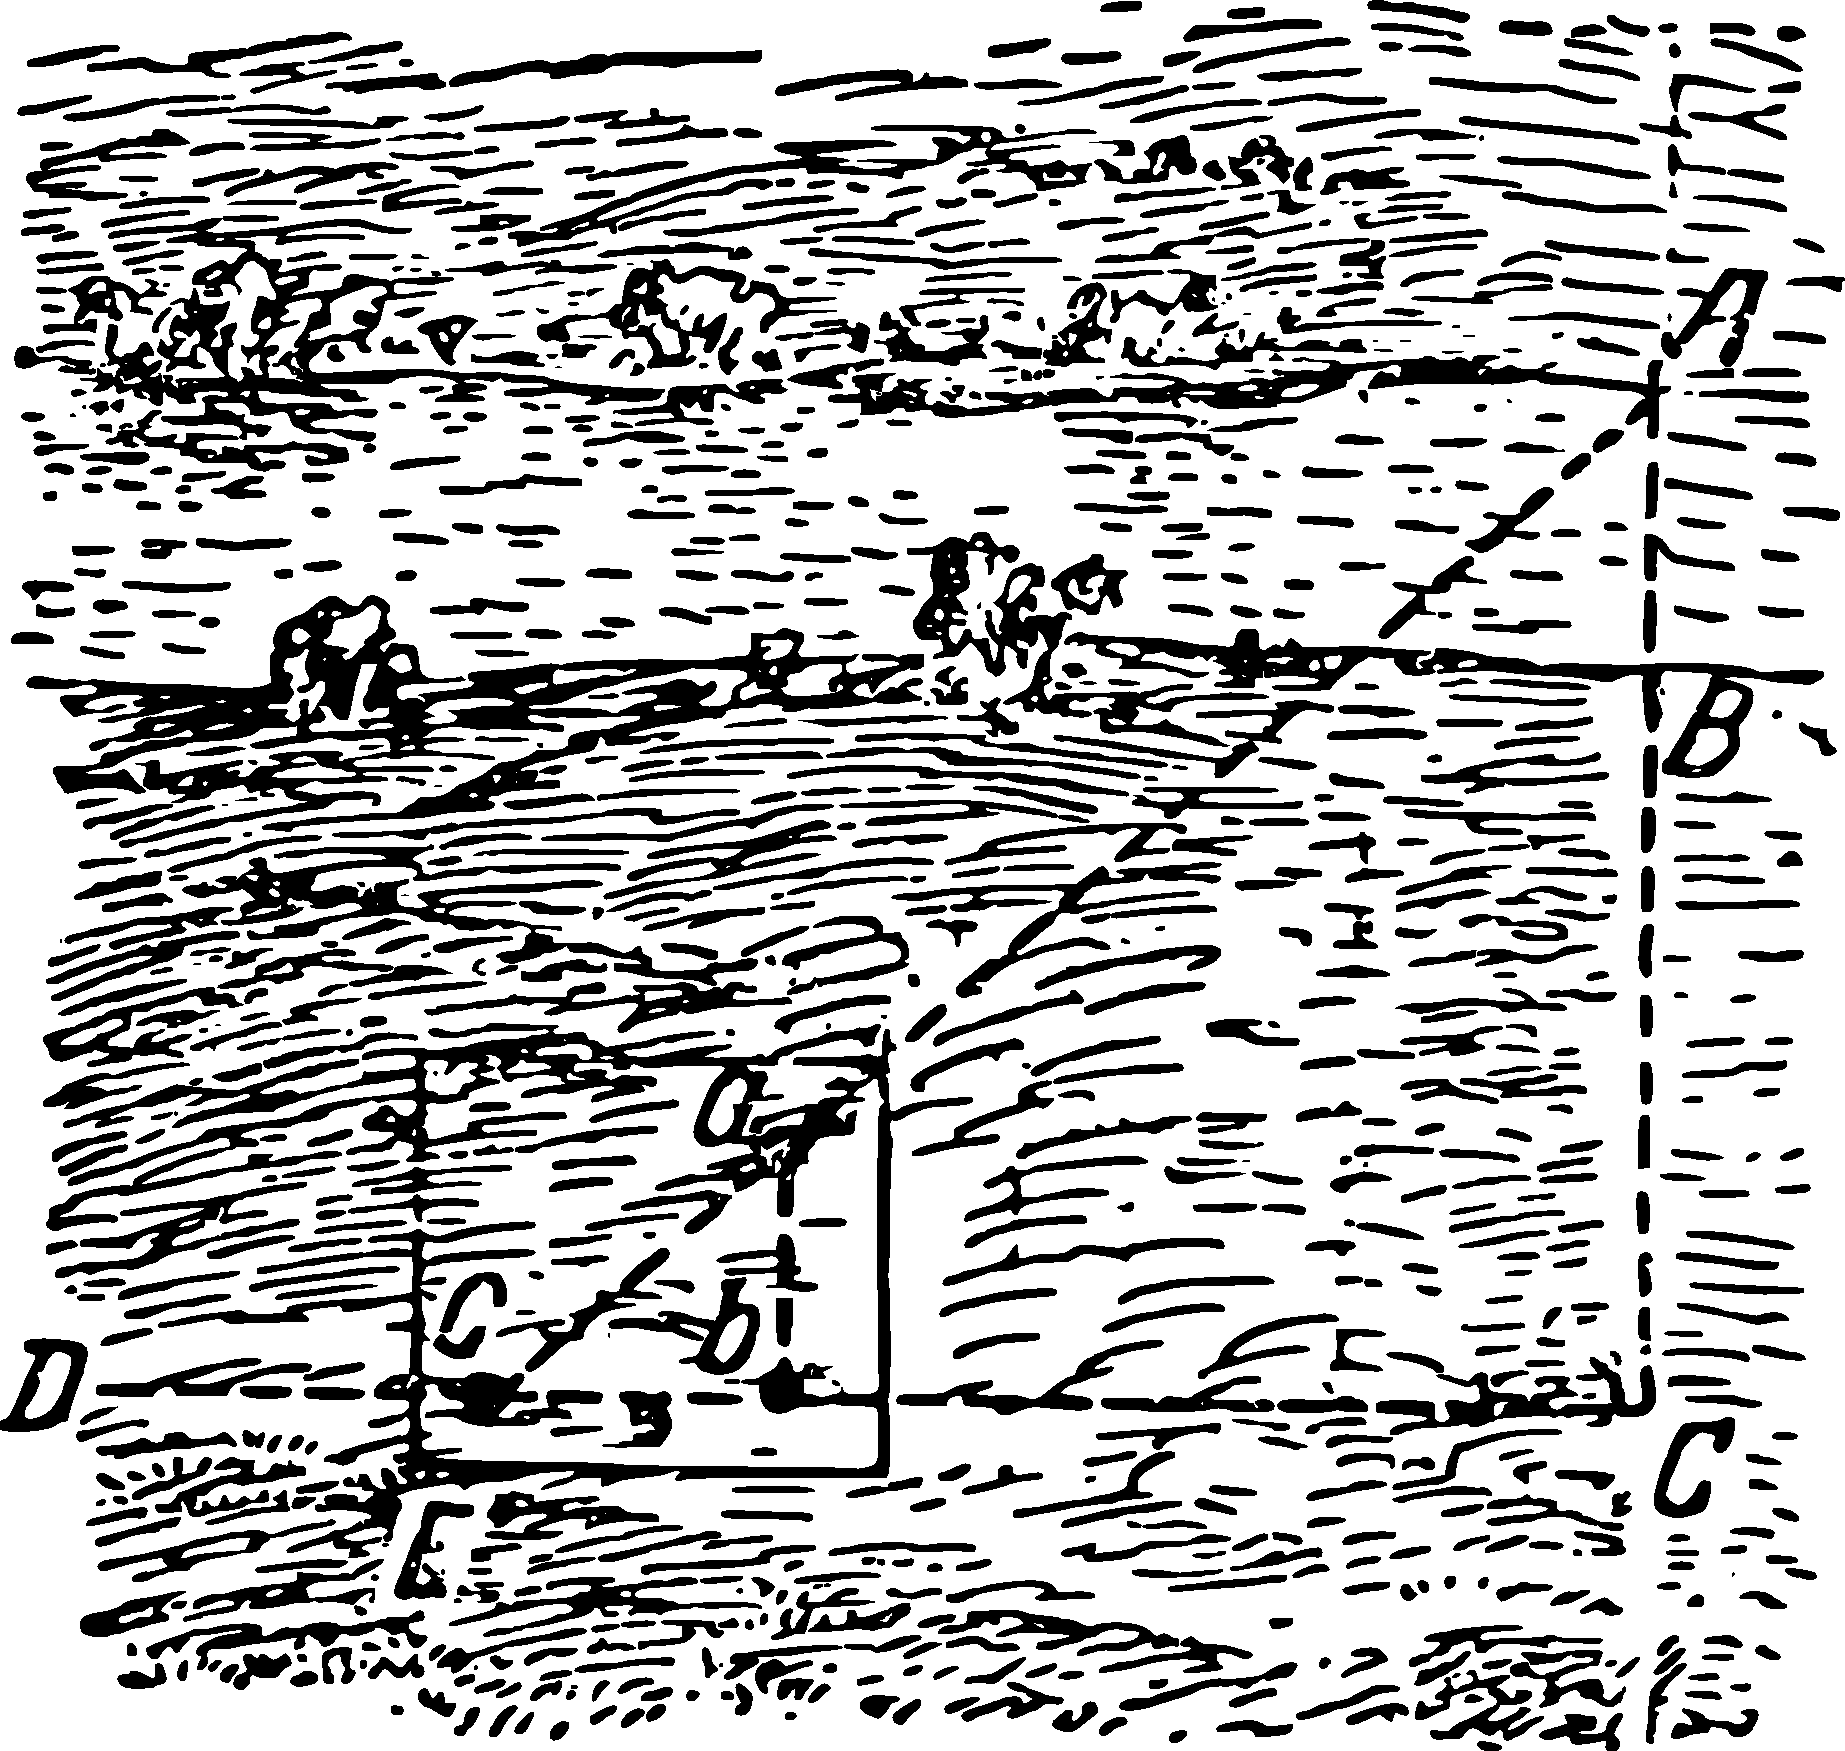
\includegraphics[width=\textwidth]{figures/ch-02/fig-027.pdf}
\sidecaption{Second position of the pin device.\label{fig-027}}
\end{marginfigure}


Now, without moving the plank of the device, look along the other two pins (perpendicular to the previous direction) and notice any point $D$ covered by these pins, i.e., lying on the line perpendicular to $AC$. After this, insert a pin at point $C$, leave this place, and go with your instrument along line $CD$ until you find a point $E$ (\figr{fig-027}), where you can simultaneously cover point $C$ for one eye with pin $b$ and point $A$ with pin $a$. This means you have found the third vertex of triangle $ACE$ on the shore, where angle $C$ is a right angle, and angle $E$ is opposite to the acute angle of the pin device, i.e., half the right angle (\ang{45}). Obviously, angle $A$ is also half right angle, i.e., $AC = CE$. If you measure the distance $CE$ even by steps, you will know the distance $AC$, and by subtracting $BC$, which is easy to measure, you will determine the desired width of the river.

It is quite inconvenient and difficult to hold the pin device still in hand; therefore, it is better to attach this plank to a stick with a pointed end and insert it vertically into the ground.

\item The second method is similar to the first. Here also, find point $C$ on the extension of $AB$ and mark line $CD$ perpendicular to $CA$ using the pin device. But then proceed differently (\figr{fig-028}). Equal distances $CE$ and $EF$ of arbitrary length are measured on the straight line $CD$, and pegs are inserted at points $E$ and $F$. Then, standing at point $F$ with a pin device, the direction $FG$ is marked out perpendicular to $FC$. Now, walking along $FG$, find a point $H$ on this line from which point $A$ seems to be covered by point $E$. This will mean that points $H$, $E$, and $A$ lie on the same straight line.

\begin{figure}[h!]
\centering
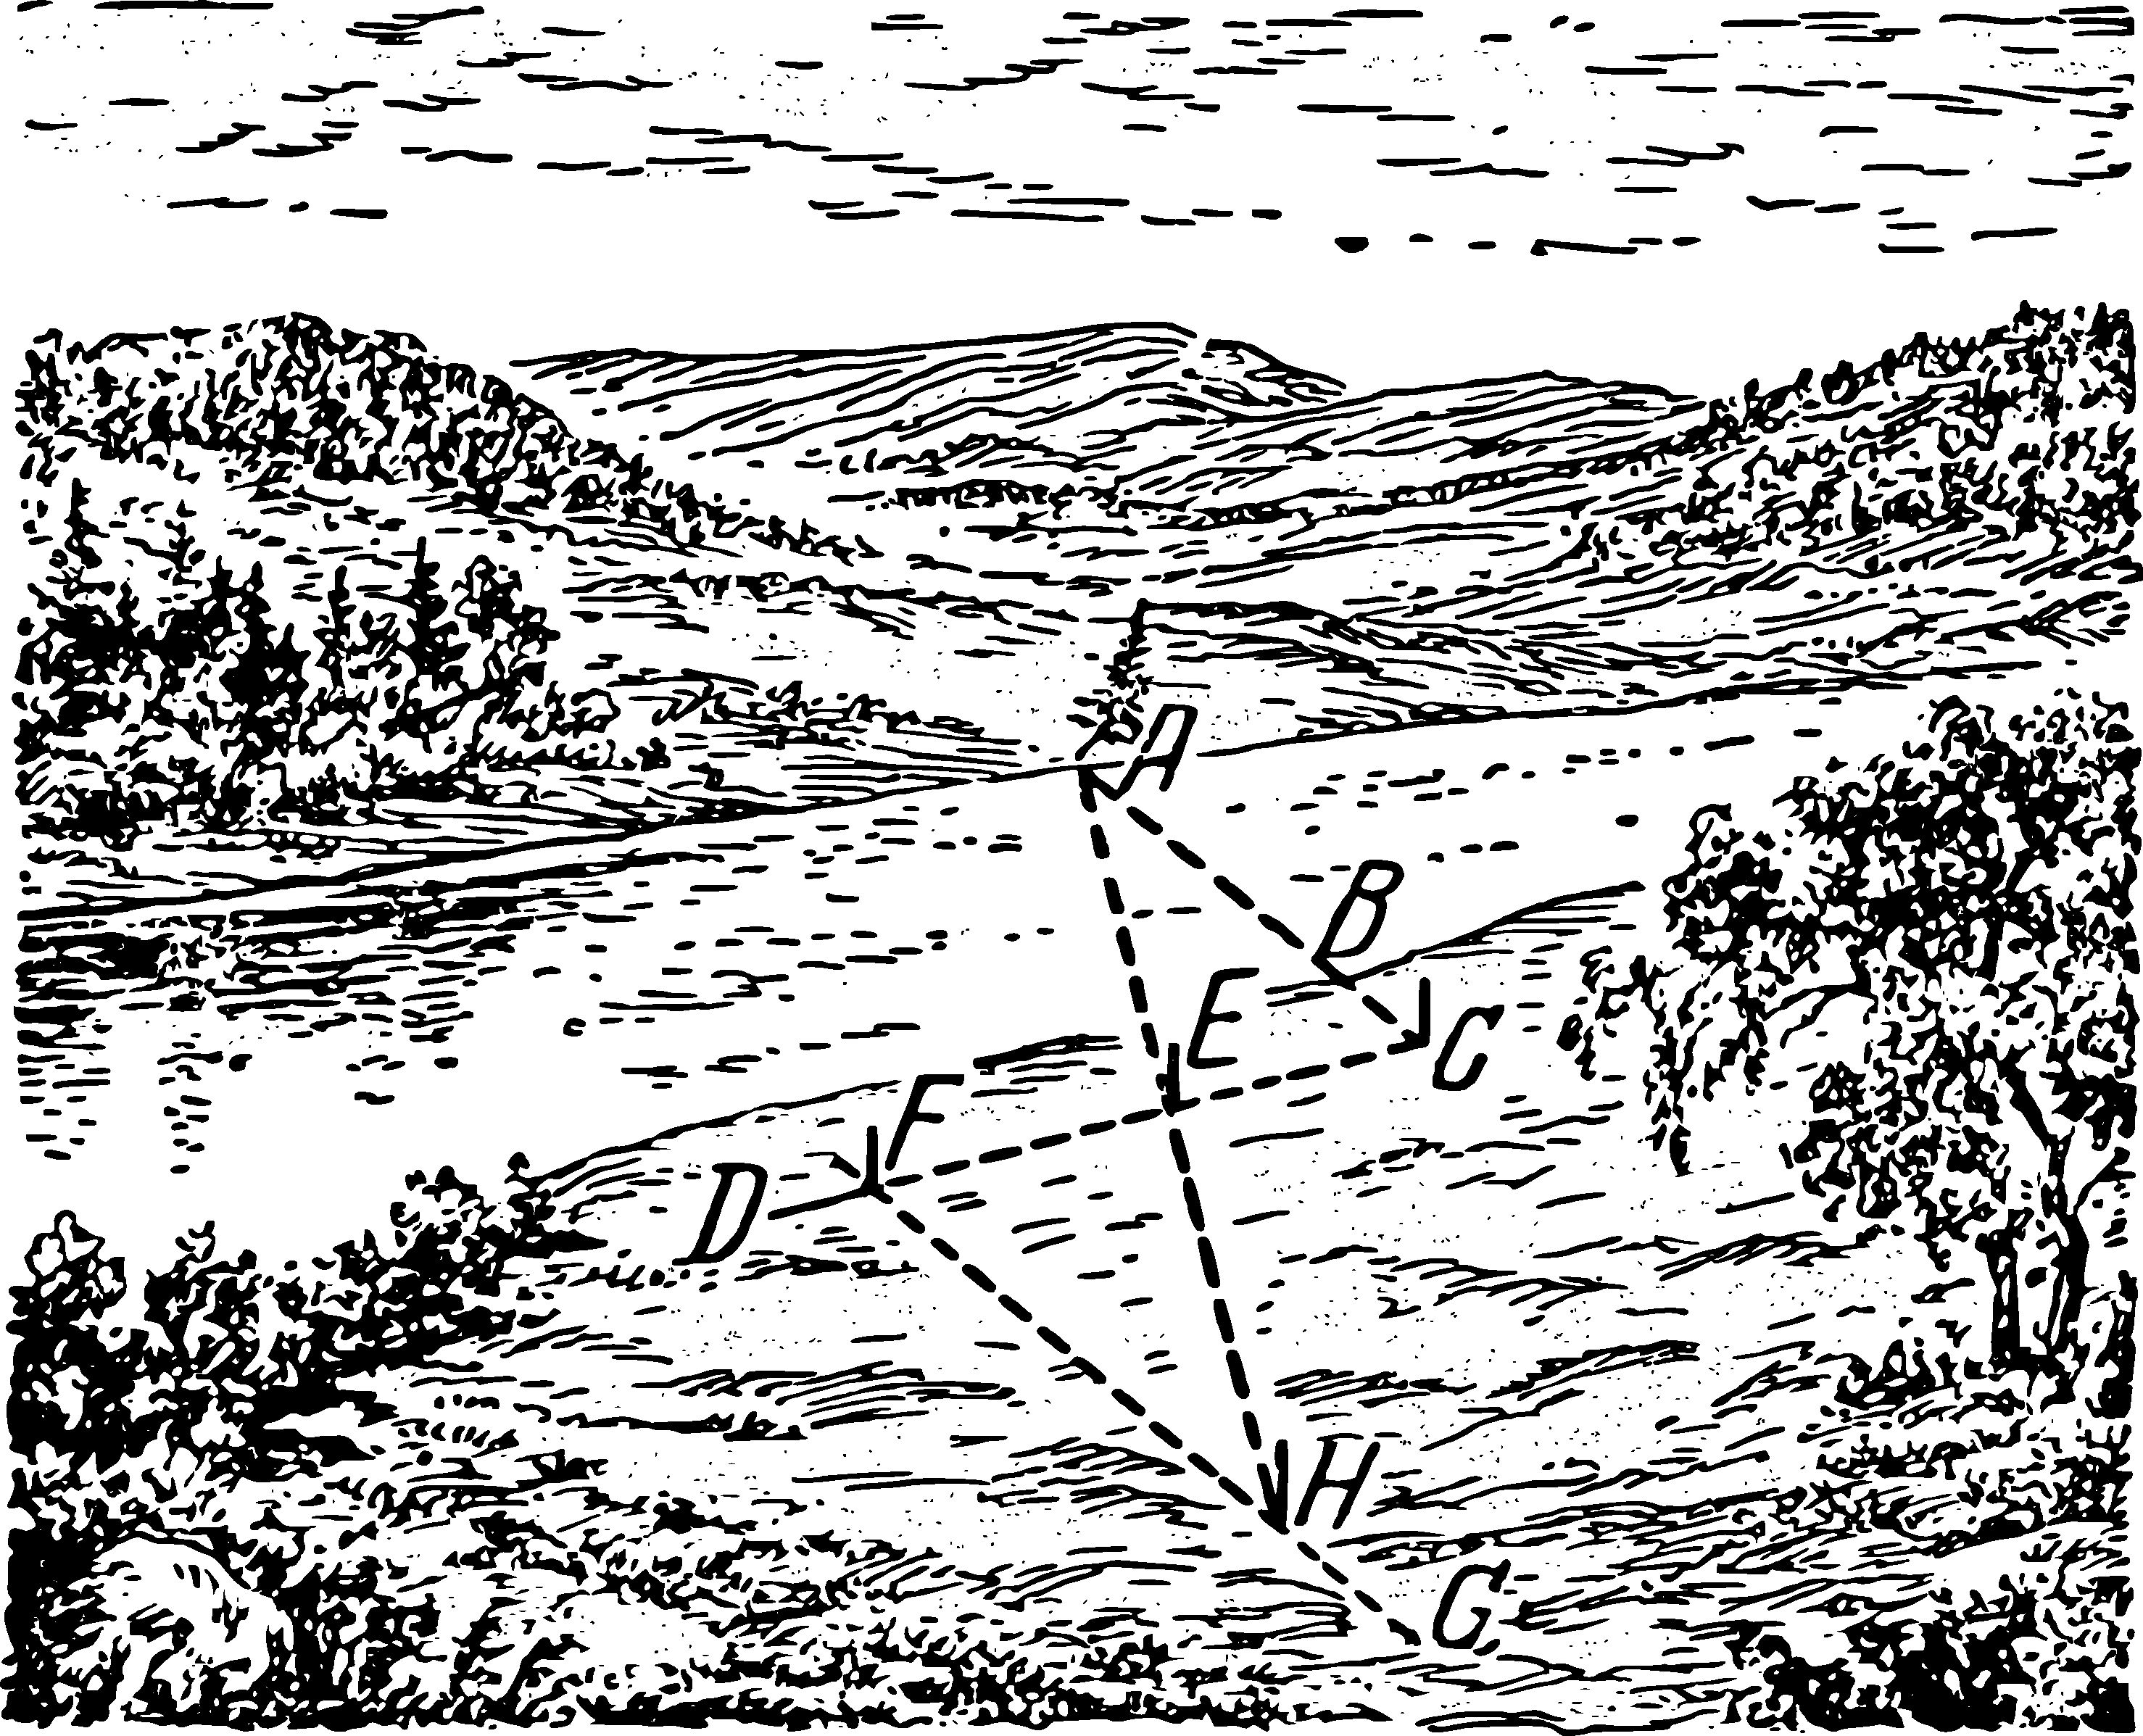
\includegraphics[width=0.9\textwidth]{figures/ch-02/fig-028.pdf}
\sidecaption{ Using the congruence criteria of triangles to find the width of the river.\label{fig-028}}
\end{figure}

The problem is solved: the distance $FH$ is equal to the distance $AC$, from which it is only necessary to subtract $BC$ to find the desired width of the river (the reader, of course, will guess for himself why $FH$ is equal to $AC$).

This method requires more space than the first one; if the terrain allows executing both methods, it is useful to verify one result by another.
\begin{figure}[h!]
\centering
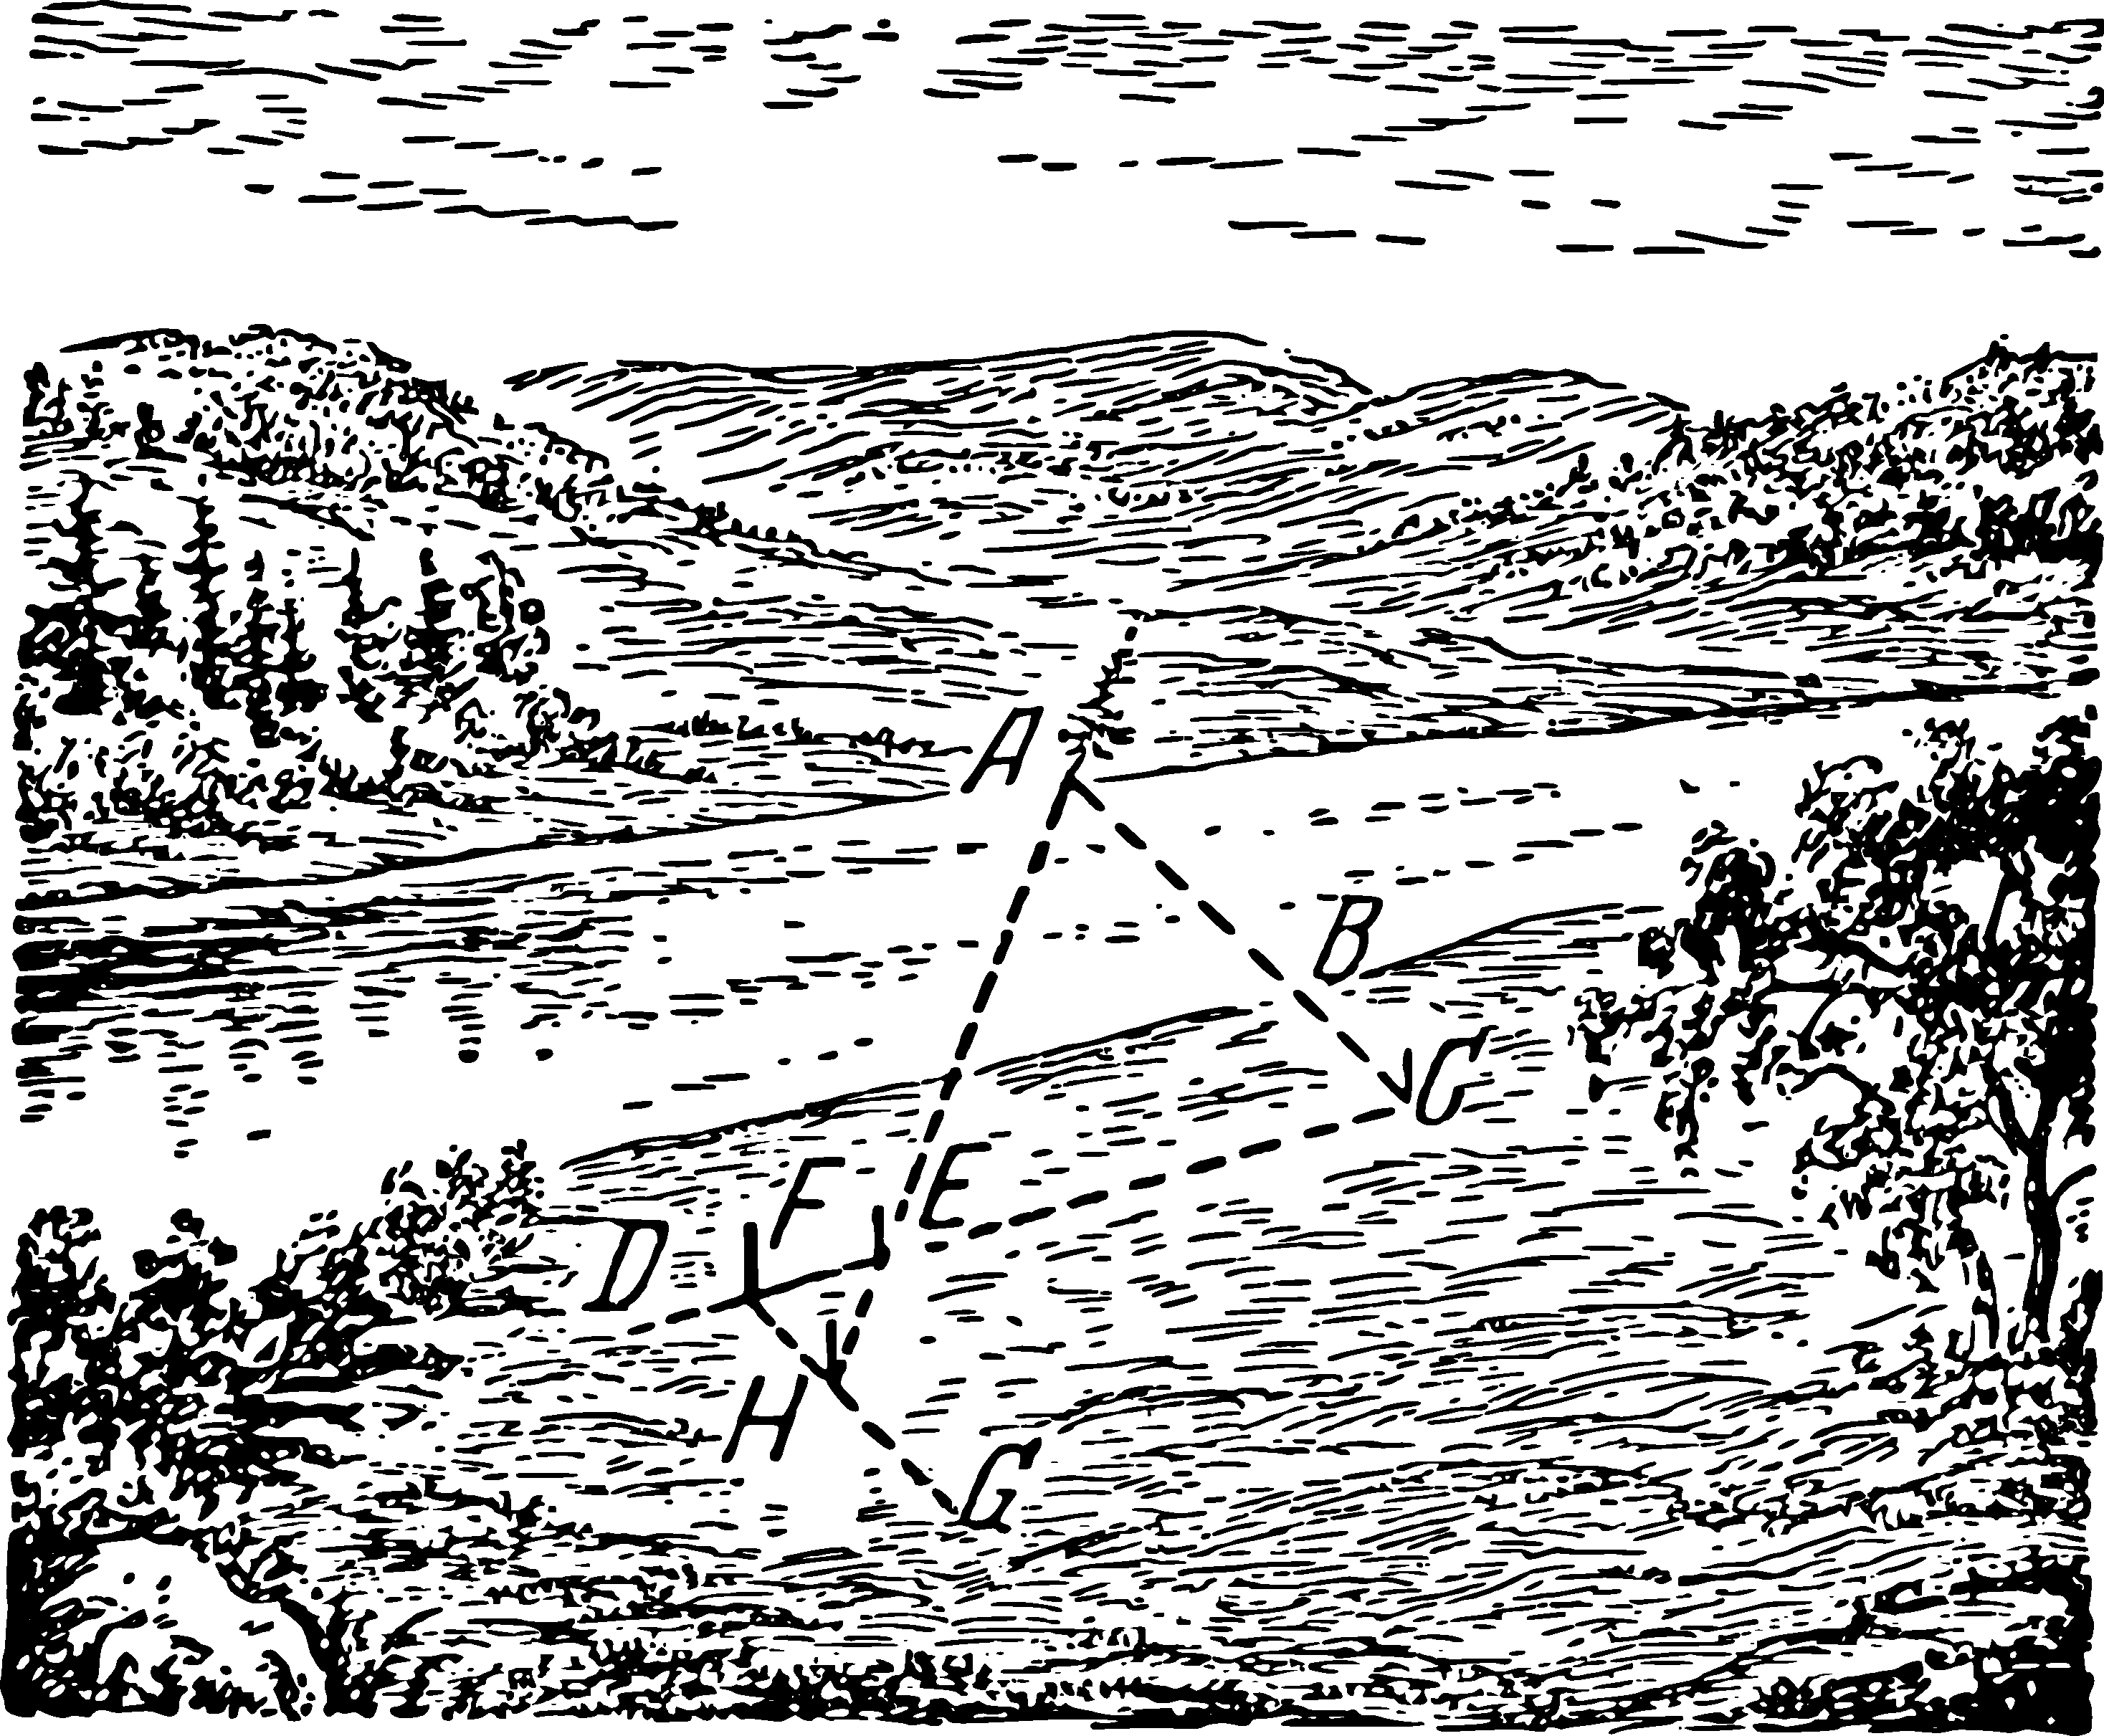
\includegraphics[width=0.9\textwidth]{figures/ch-02/fig-029.pdf}
\sidecaption{Using the similarity criteria of triangles to find the width of the river.\label{fig-029}}
\end{figure}

\item The method described above can be modified: instead of measuring equal distances on the straight line $CF$, measure one distance several times smaller than the other. For example (\figr{fig-029}), $FE$ is measured four times less than $EC$, and then we proceed as before: in the direction $FG$, perpendicular to $FC$, we find a point $H$ from which the peg $E$ appears to cover point $A$. But now $FH$ is no longer equal to $AC$, but four times smaller than this distance: triangles $ACE$ and $EFH$ are not congruent here, but similar (they have equal angles with unequal sides). From the similarity of triangles follows the proportion:
\begin{equation*}%
\frac{AC}{FH} = \frac{CE}{EF} = \frac{4}{1}
\end{equation*}
Therefore, by measuring $FH$ and multiplying the result by 4, we get the distance $AC$, and by subtracting $BC$, we find the desired width of the river.

This method, as we can see, requires less space and is therefore more convenient to perform than the previous one.




\item The fourth method is based on the property of a right triangle that if one of its acute angles is \ang{30}, then the length of the cathetus is half the hypotenuse. It is very easy to verify the correctness of this. 

Let angle $B$ of right triangle $ABC$ (\figr{fig-030}, left) be \ang{30}; we will prove that in this case, $AC = \nicefrac{1}{2}\, AB$. Rotate triangle $ABC$ around $BC$ so that it is symmetric with its initial position (\figr{fig-030}, right), forming figure $ABD$; line $AC$ is straight because both angles at point $C$ are right angles. In triangle $ABD$, angle $\angle A = \ang{60}$, angle $ABD$, composed of two \ang{30} angles, is also equal to \ang{60}. Therefore, $AD = BD$ as sides opposite equal angles. But $AC = \nicefrac{1}{2} \,AD$, therefore,
\begin{marginfigure}%[5cm]%[h!]
\centering
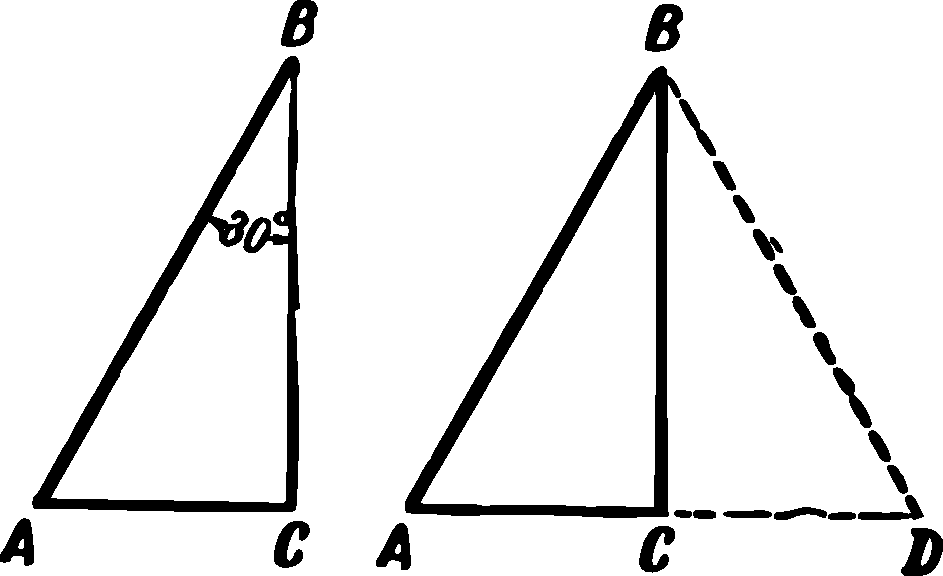
\includegraphics[width=\textwidth]{figures/ch-02/fig-030.pdf}
\sidecaption{When the cathetus is half the hypotenuse.\label{fig-030}}
\end{marginfigure}
\begin{equation*}%
AC = \frac{1}{2} AB.
\end{equation*}
Wishing to take advantage of this property of the triangle, we must arrange the pins on the board so that their bases represent a right triangle in which the cathetus is half the hypotenuse. With this device, we place ourselves at point $C$ (\figr{fig-031}) so that the direction $AC$ coincides with the hypotenuse of the pin triangle. 
\begin{marginfigure}%[5cm]%[h!]
\centering
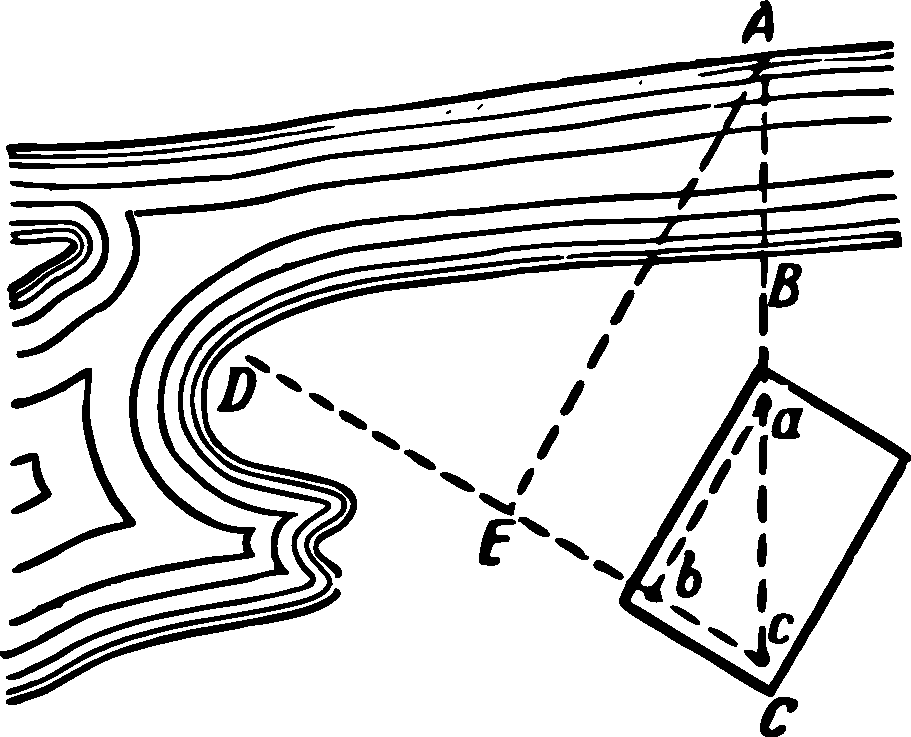
\includegraphics[width=\textwidth]{figures/ch-02/fig-031.pdf}
\sidecaption{The scheme of application of a right-angled triangle with a 30° angle.\label{fig-031}}
\end{marginfigure}
Looking along the short cathetus of this triangle, mark the direction $CD$ and find a point $E$ on it so that the direction $EA$ is perpendicular to $CD$ (this is done using the same pin device). It is easy to see that the distance $CE$ -- the cathetus lying opposite the angle of \ang{30} -- is equal to half of $AC$. Therefore, by measuring $CE$, doubling this distance and subtracting $BC$, we obtain the desired width of the $AB$ river.

\end{enumerate}

Here are four easily executable methods, with which it is always possible, without crossing to the other bank, to measure the width of the river with quite satisfactory accuracy. We will not consider methods that require the use of more complex instruments (even homemade ones) here.

\section{Using a visor}
\label{sec-2.2}

Here's how this method came in handy for Senior Sergeant Kupriyanov in frosty conditions.\sidenote{See the footnote on page~\pageref{ref-21}.} His detachment was ordered to measure the width of the river, across which they were to organise a crossing\ldots{}

Approaching a bush near the river, Kupriyanov's detachment took cover, and Kupriyanov himself, along with soldier Karpov, moved closer to the riverbank, from where the fascist-occupied shore was clearly visible. In such conditions, measuring the width of the river had to be done by eye.

``Come on, Karpov, how much?'' Kupriyanov asked.

``I think no more than 100-110 meters,'' Karpov replied. Kupriyanov agreed with his scout, but for control, he decided to measure the width of the river using a ``visor.''

\begin{figure}[h!]
\centering
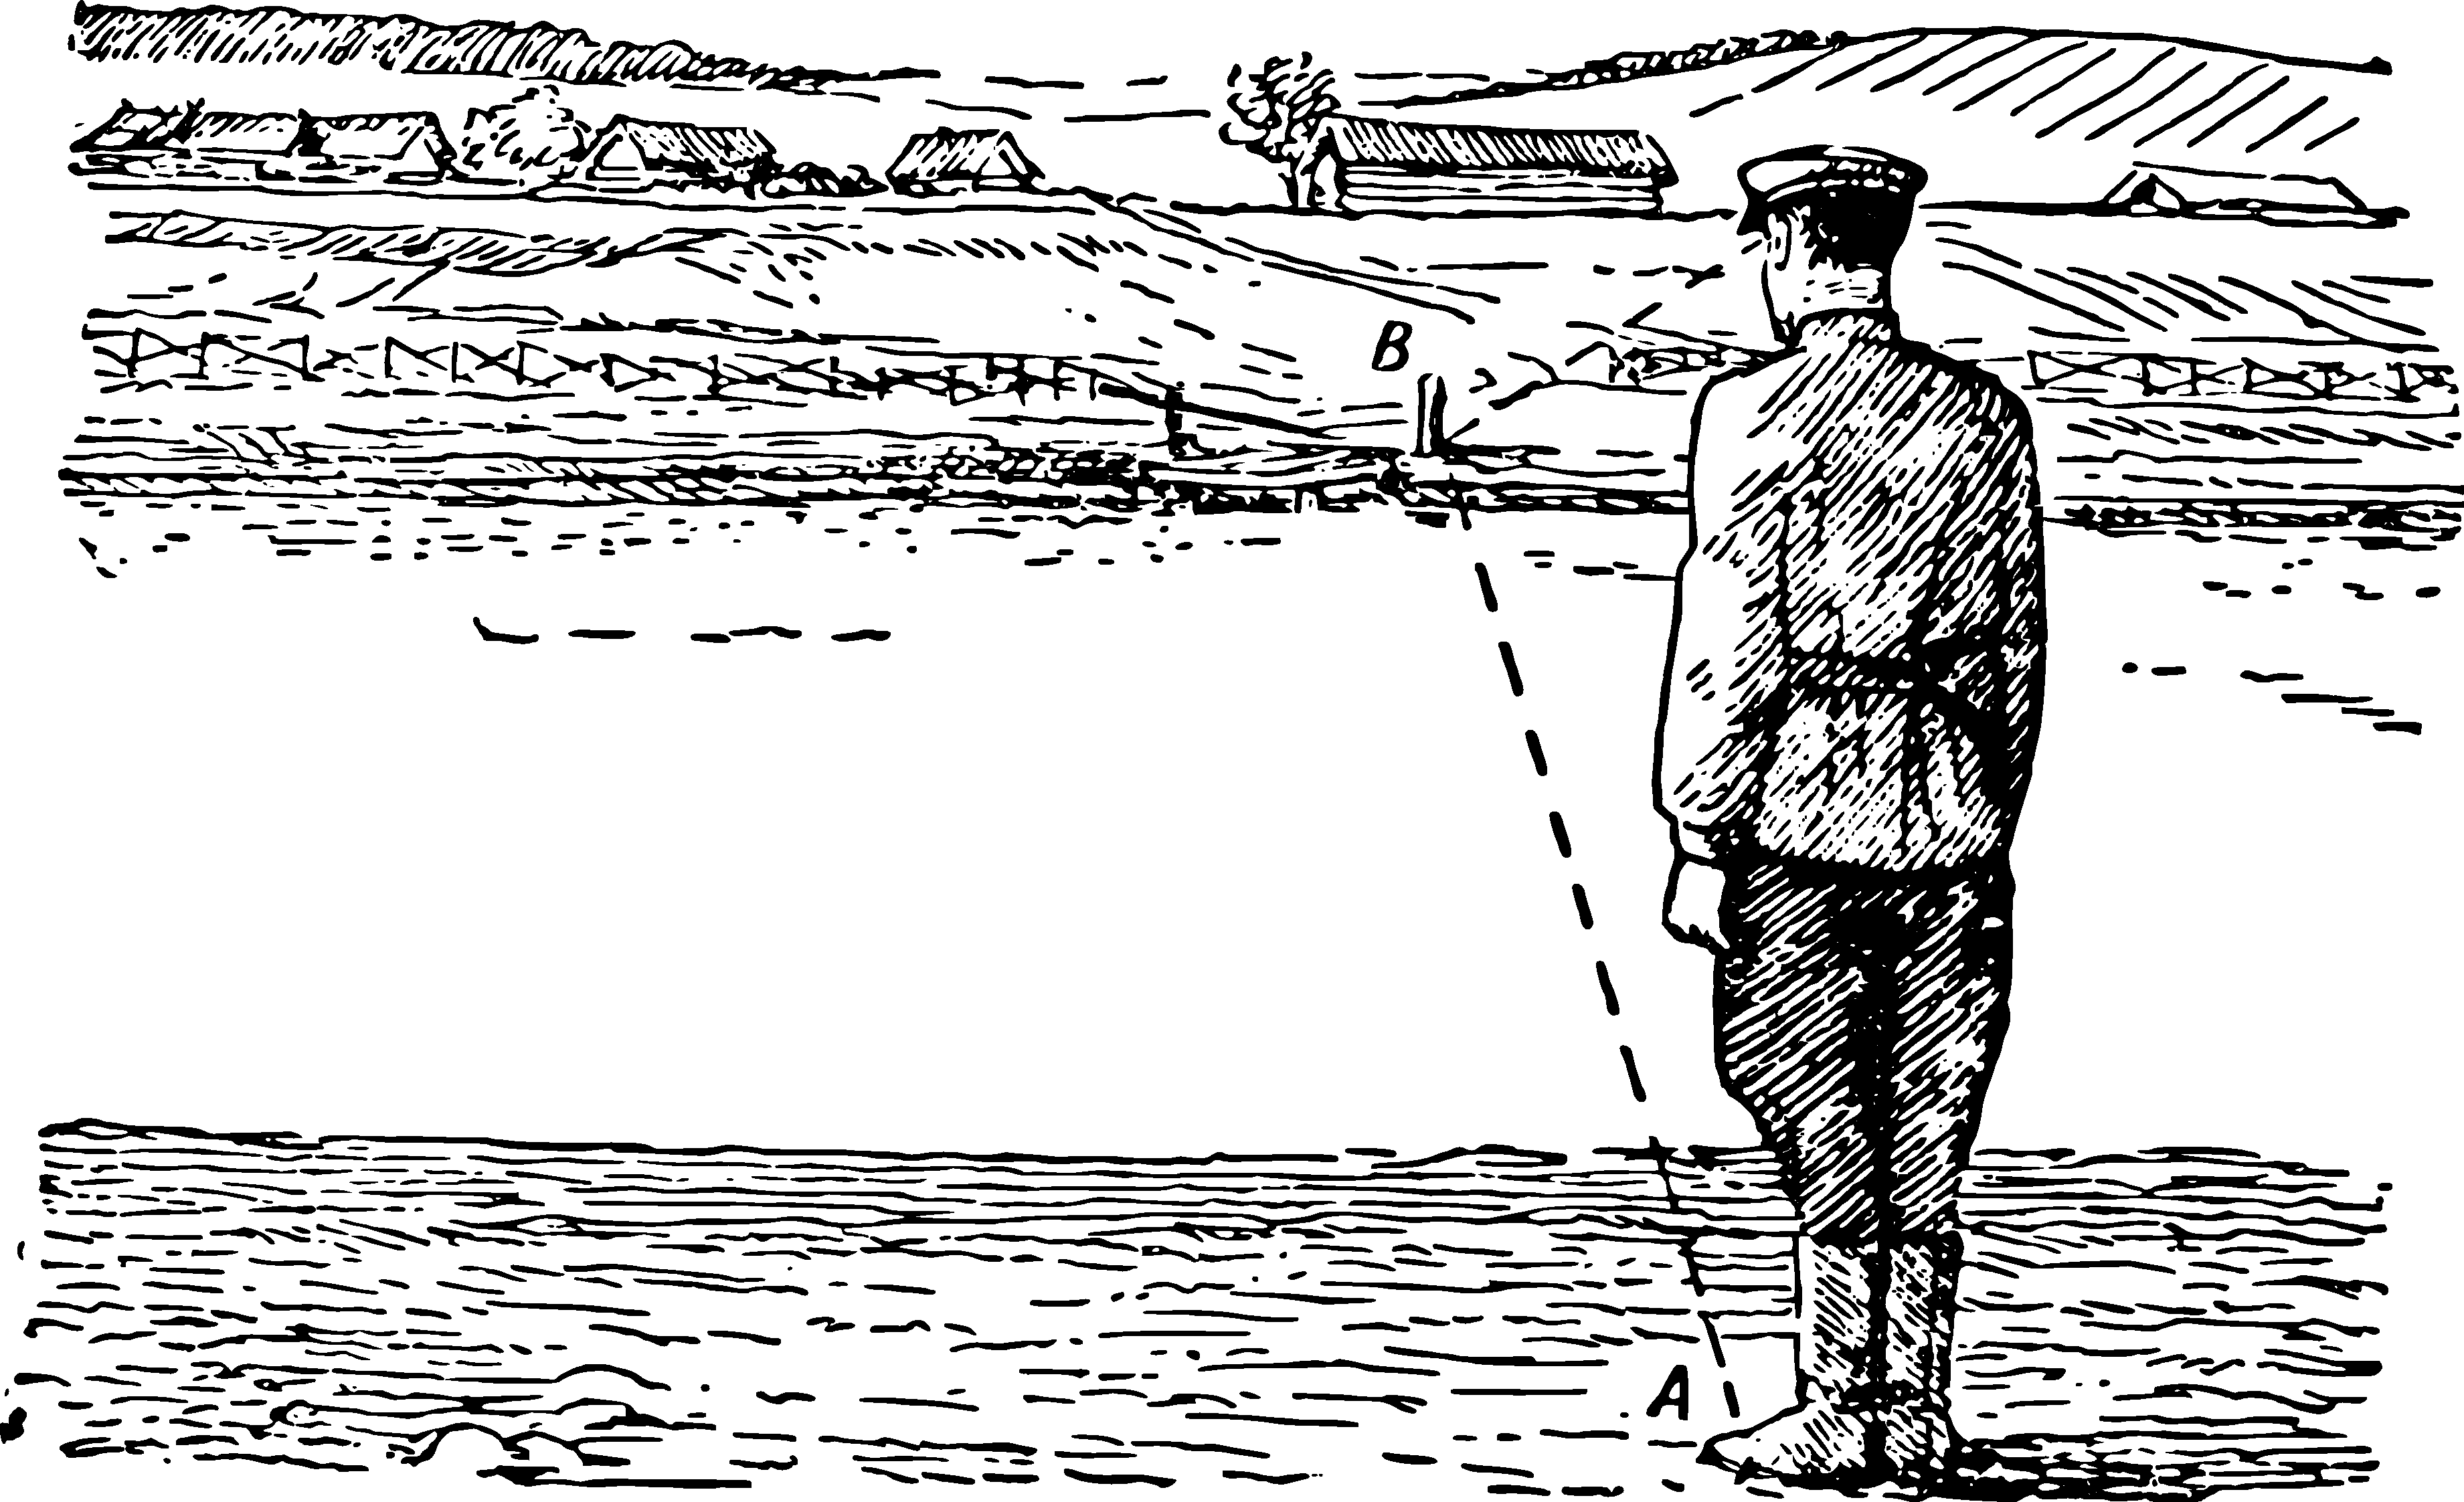
\includegraphics[width=0.9\textwidth]{figures/ch-02/fig-032.pdf}
\sidecaption{Observing a point on the opposite bank from under the visor.\label{fig-032}}
\end{figure}

This method is simple. You have to face the river and pull the visor over your eyes so that the lower edge of the visor precisely aligns with the line of the opposite bank (see \figr{fig-032}). The visor can be replaced with the palm of your hand or a notepad, tightly pressed edge to your forehead. Then, without changing the position of your head, you need to turn to the right or left, or even backward (towards the side where the area available for measuring the distance is more level) and notice the farthest point visible from under the visor (palm, notepad).

The distance to this point will be approximately equal to the width of the river.

Kupriyanov utilized this method. He quickly stood up in the bushes, pressed a notepad to his forehead, then quickly turned and aimed at the distant point. Then, together with Karpov, he crawled to that point, measuring the distance with a rope. It turned out to be 105 meters.

Kupriyanov reported the data he obtained to the command.

\ques Provide a geometric explanation for the ``visor'' method.

\begin{figure}[h!]
\centering
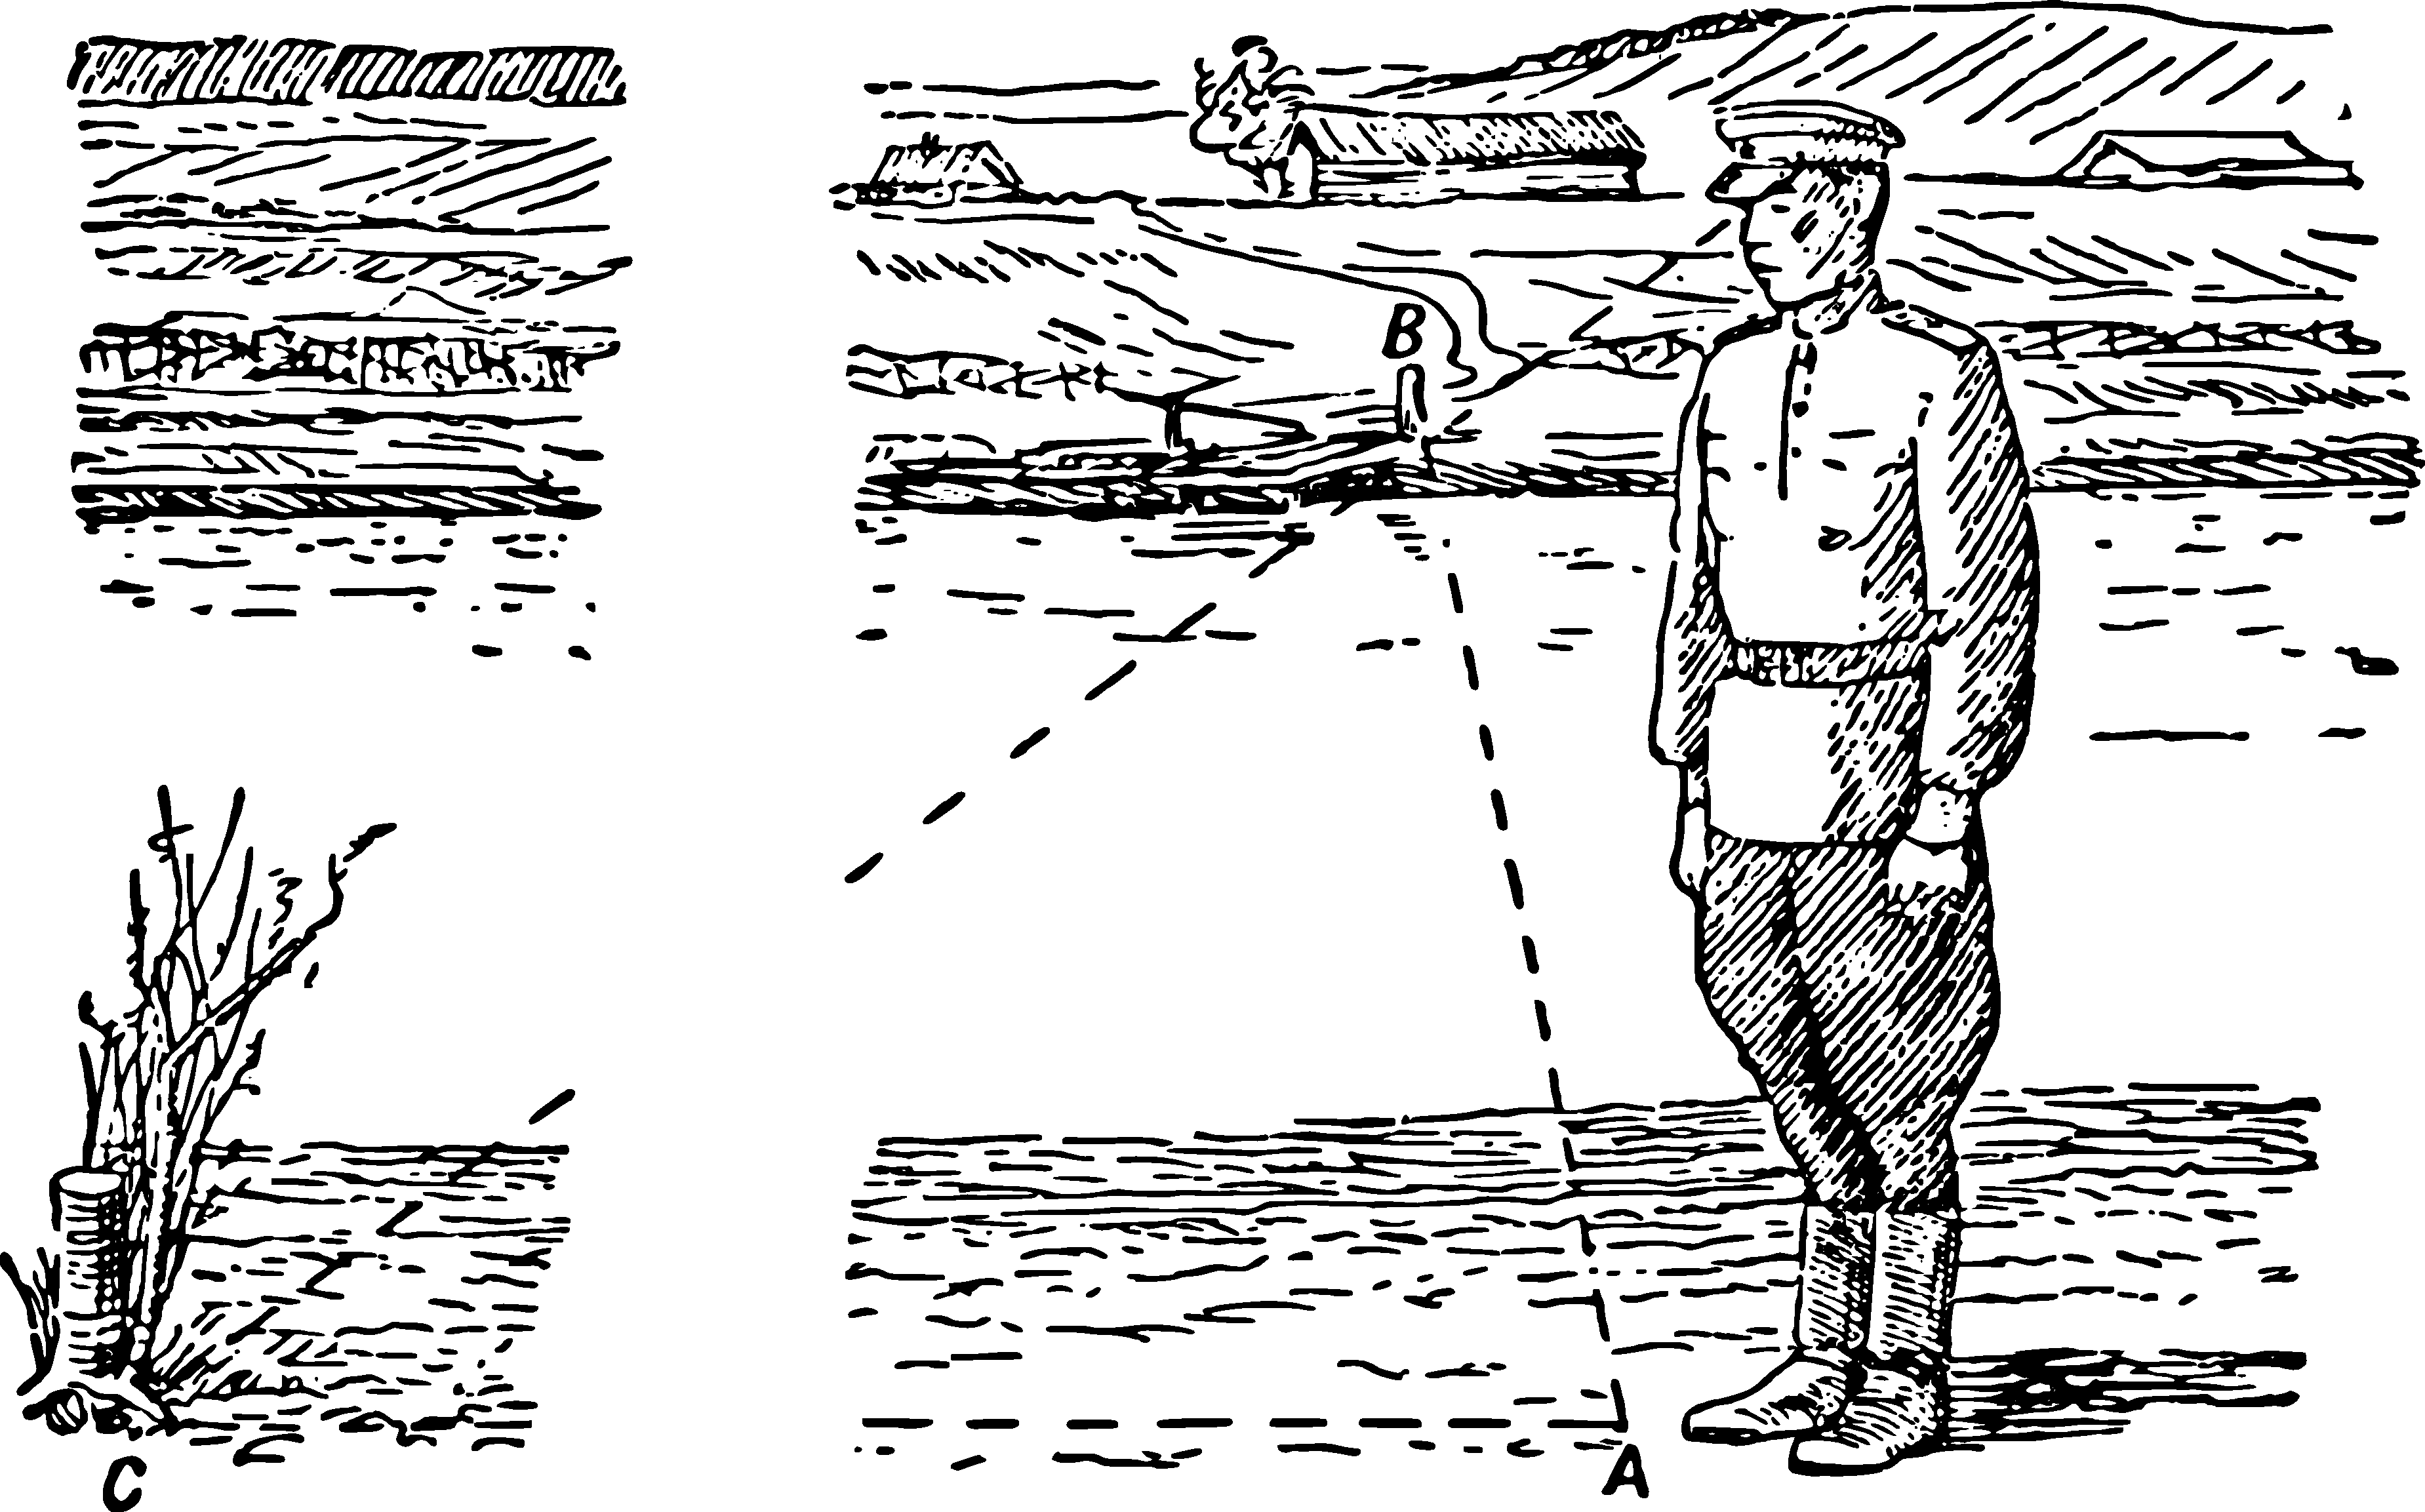
\includegraphics[width=0.9\textwidth]{figures/ch-02/fig-033.pdf}
\sidecaption{In the same way, you can aim at a point on your own bank.\label{fig-033}}
\end{figure}

\ans The line of sight, touching the edge of the visor (palm, notepad), is initially directed towards the line of the opposite bank (see \figr{fig-032}). When a person turns, the line of sight, like the leg of a compass, describes a circle, and then $AC = AB$ as the radii of the same circle (see \figr{fig-033}). 

\section{The Length Of An Island}

\ques Now we are faced with a more challenging task. Standing by the river or lake, you see an island (see \figr{fig-034}) whose length you wish to measure without leaving the shore. Is it possible to carry out such a measurement?

Although in this case, both ends of the measured line are inaccessible to us, the problem is still entirely solvable, and without complex instruments.

\begin{figure}[h!]
\centering
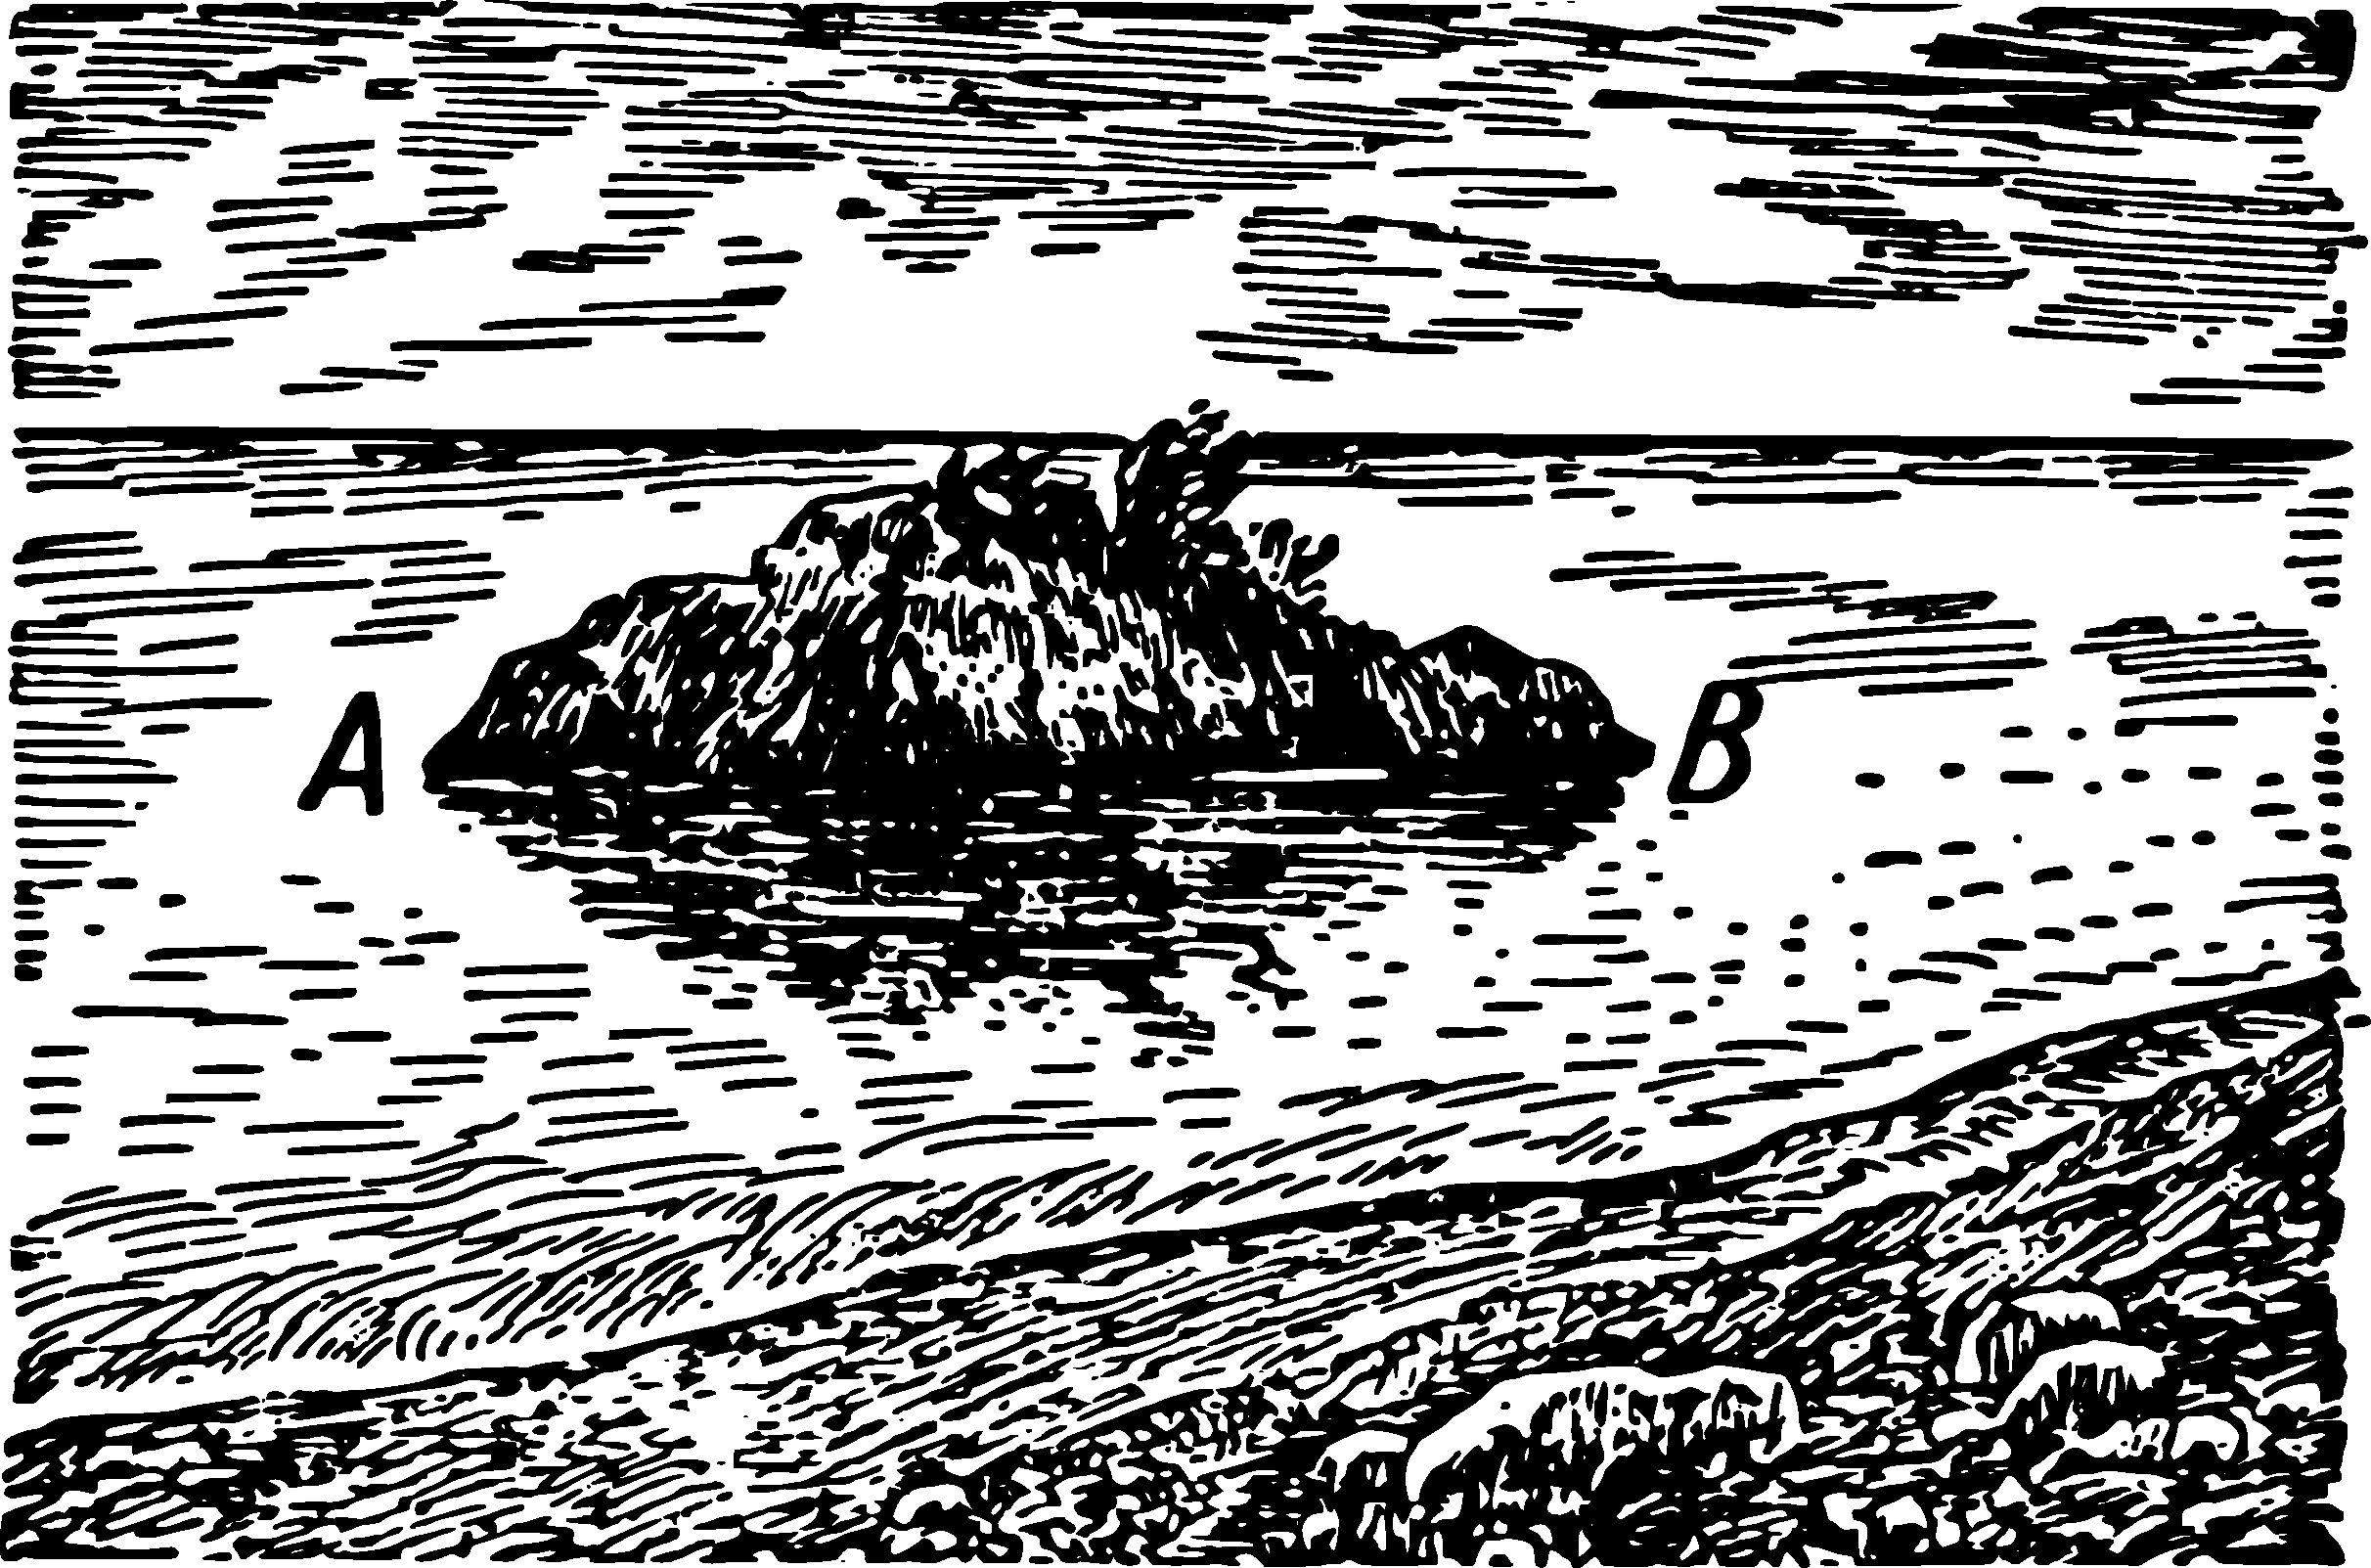
\includegraphics[width=0.9\textwidth]{figures/ch-02/fig-034.pdf}
\sidecaption{How to determine the length of the island.\label{fig-034}}
\end{figure}


\ans To measure the length of an island without leaving the shore, you can use the following method. Choose arbitrary points $P$ and $Q$ on the shore and place stakes in them. Then find points $M$ and $N$ on the line $PQ$ such that the directions $AM$ and $BM$ form right angles with the direction of $PQ$ (this can be done using a compass). In the middle of the distance $MN$, place a stake $O$ and find on the extension of the line $AM$ a point $C$ from which the stake $O$ appears to cover point $B$. Similarly, on the extension of $BN$, find point $D$ from which stake $O$ appears to cover the end $A$ of the island. The distance $CD$ will be the desired length of the island.

\begin{marginfigure}[-3cm]%[h!]
\centering
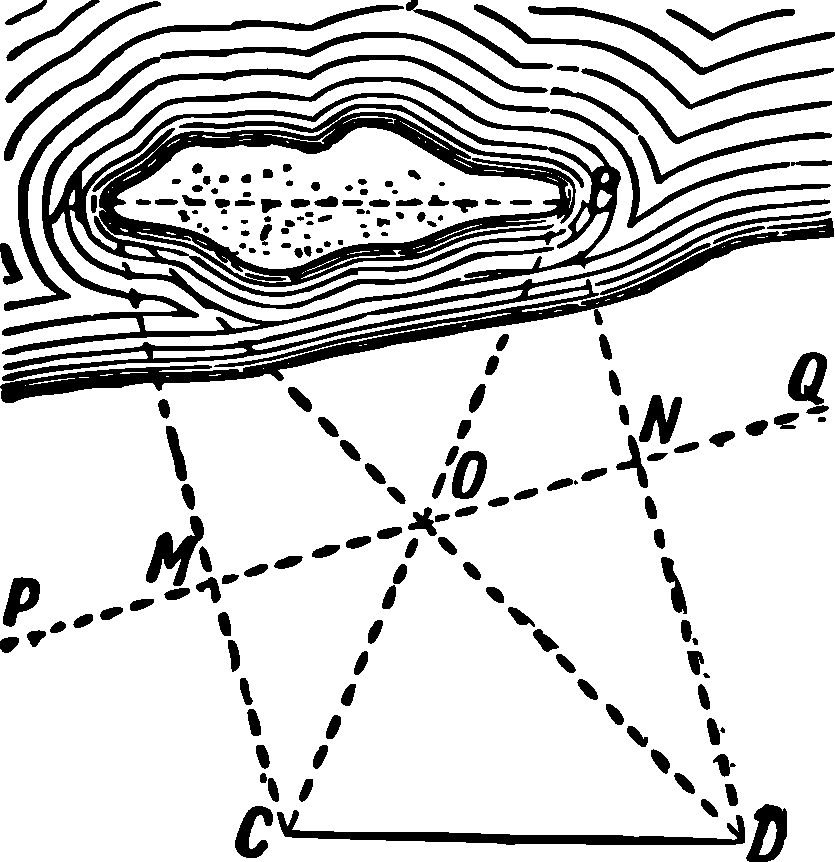
\includegraphics[width=\textwidth]{figures/ch-02/fig-035.pdf}
\sidecaption{We use the properties of congruent right triangles to find the length of an isalnd.\label{fig-035}}
\end{marginfigure}

This can be easily proved. Consider the right triangles $AMO$ and $OND$; in them, the legs $MO$ and $NO$ are equal, and the angles $AOM$ and $NOD$ are also equal, therefore, the triangles are equal, and $AO = OD$. Similarly, it can be proved that $BO = OC$. By comparing the triangles $ABO$ and $COD$, it can be seen that their distances $AB$ and $CD$ are equal.

\section{A pedestrian on the opposite bank}
\label{sec-2.3}

\ques As you walk along the riverbank, you see a person on the other side, and you can clearly distinguish their steps. Can you, without moving from your spot, determine at least approximately the distance between them and you? You have no instruments at hand.

\begin{figure}[h!]
\centering
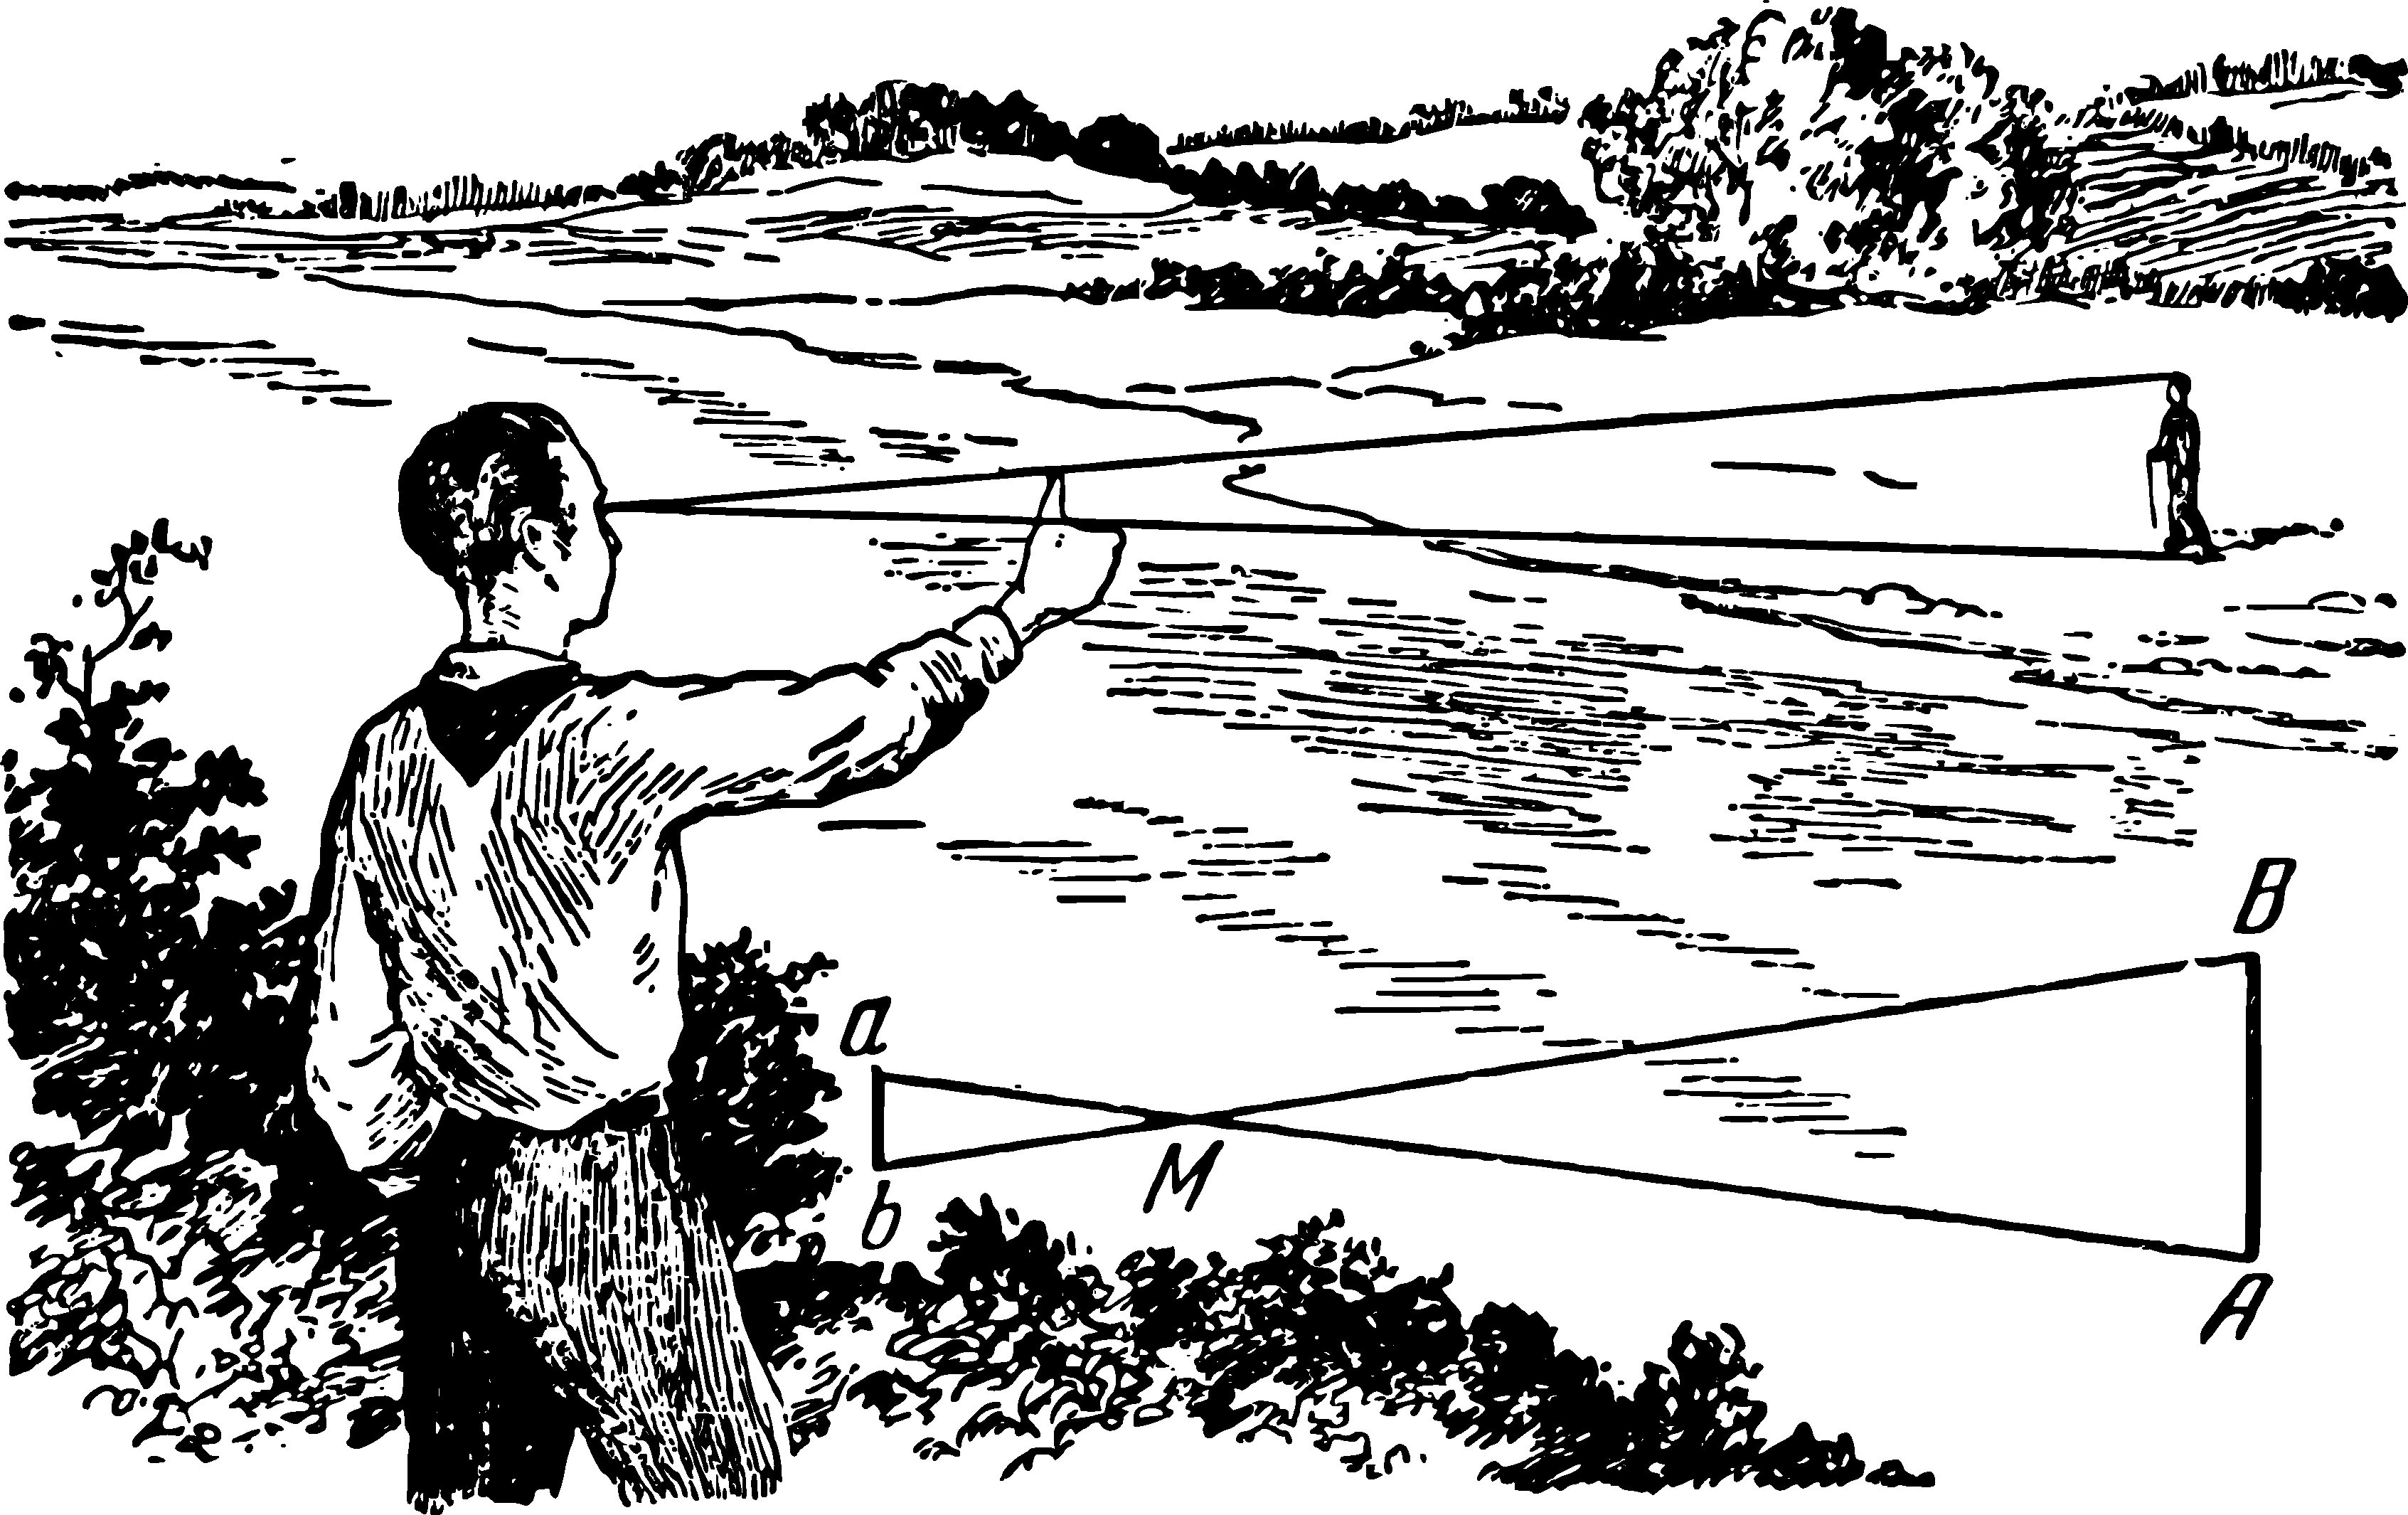
\includegraphics[width=0.9\textwidth]{figures/ch-02/fig-036.pdf}
\sidecaption{How to determine the distance to a pedestrian walking on the other side of the river.\label{fig-036}}
\end{figure}


\ans You don't have any instruments, but you have eyes and hands -- that's enough. Extend your arm forward towards the pedestrian and look at the tip of your finger with one eye if the pedestrian is moving towards your right hand, and with the other eye if they're moving towards your left hand. At the moment when the distant pedestrian is covered by your finger (see \figr{fig-036}), close the eye that was looking and open the other: the pedestrian will appear to you as if they've moved backward. Count how many steps they take before they align again with your finger. You'll get all the data needed for an approximate determination of the distance. Let's explain how to use them.

Suppose in \figr{fig-036} (inset), your eyes are marked as $a$ and $b$, point $M$ is the tip of your finger extended, point $A$ is the initial position of the pedestrian, and $B$ is the final position. The triangles $abM$ and $ABM$ are similar (you should turn towards the pedestrian so that $ab$ is approximately parallel to their direction of movement). Therefore, $BM : bM = AB : ab$ -- is a proportion in which only one term, $BM$, is unknown, but all others can be directly determined. Indeed, $bM$ is the length of your extended arm, $ab$ is the distance between the pupils of your eyes, and $AB$ is measured in steps taken by the pedestrian (assuming an average step to be around 3/4 metres). Therefore, the unknown distance from you to the pedestrian on the opposite bank, $AB$, equals 
\begin{equation*}%
MB = AB \, \frac{bM}{ab}
\end{equation*}
For example, if the distance between your eye pupils $ab$ is \SI{6}{\centi\meter}, the length of $bM$ from the end of your extended arm to the eye is \SI{60}{\centi\meter}, and the pedestrian takes, say, 14 steps from $A$ to $B$, then their distance from you would be $MB = 14 \cdot 60/6 = 140$ steps, or 105 meters.

It's enough for you to measure in advance the distance between your eye pupils and $bM$ -- the distance from the eye to the end of your extended arm -- so that you can quickly determine the distance of inaccessible objects by remembering their ratio. On average, for most people, $bM/ab$ is around 10 with slight fluctuations. The difficulty will only be in somehow determining the distance $AB$. In our case, we used the steps of a distant person. But you can also use other references. For instance, if you're measuring the distance to a distant freight train, you can estimate $AB$ in comparison to the length of a freight car, which is usually known (7.6 meters between buffers). If you're determining the distance to a house, you can estimate $AB$ by comparing it to the width of a window, the length of a brick, etc.

The same method can be applied to determine the size of a distant object if its distance from the observer is known. For this purpose, you can also use other ``rangefinders'', which we will describe next.

\section{Simple Rangefinders}
\begin{marginfigure}[-2cm]%[h!]
\centering

\includegraphics[width=0.1\textwidth]{figures/ch-02/fig-037.pdf}
\sidecaption{The match is a rangefinder.\label{fig-037}}
\end{marginfigure}
In the first chapter, we described the simplest instrument for determining inaccessible heights -- the altimeter. Now, let's describe the simplest device for measuring inaccessible distances -- the `rangefinder.' The simplest rangefinder can be made from an ordinary matchstick. To do this, you just need to mark millimeter divisions on one of its sides, alternating between light and dark (see \figr{fig-037}).


You can use this primitive ``rangefinder'' to estimate the distance to a distant object only in those cases when the dimensions of that object are known to you (see \figr{fig-038}). However, more sophisticated rangefinders can also be used under the same condition. Suppose you see a person in the distance and set yourself the task of determining the distance to them. Here, the matchstick rangefinder can come in handy. Holding it in your outstretched arm and looking with one eye, you bring its free end into coincidence with the top of the distant figure. Then, slowly moving your thumbnail along the matchstick, you stop it at the point that projects onto the base of the human figure. All you have to do now is to find out, by bringing the matchstick closer to the eye, at which mark your thumbnail stopped -- and then you have all the data to solve the problem.

\begin{figure}[h!]
\centering
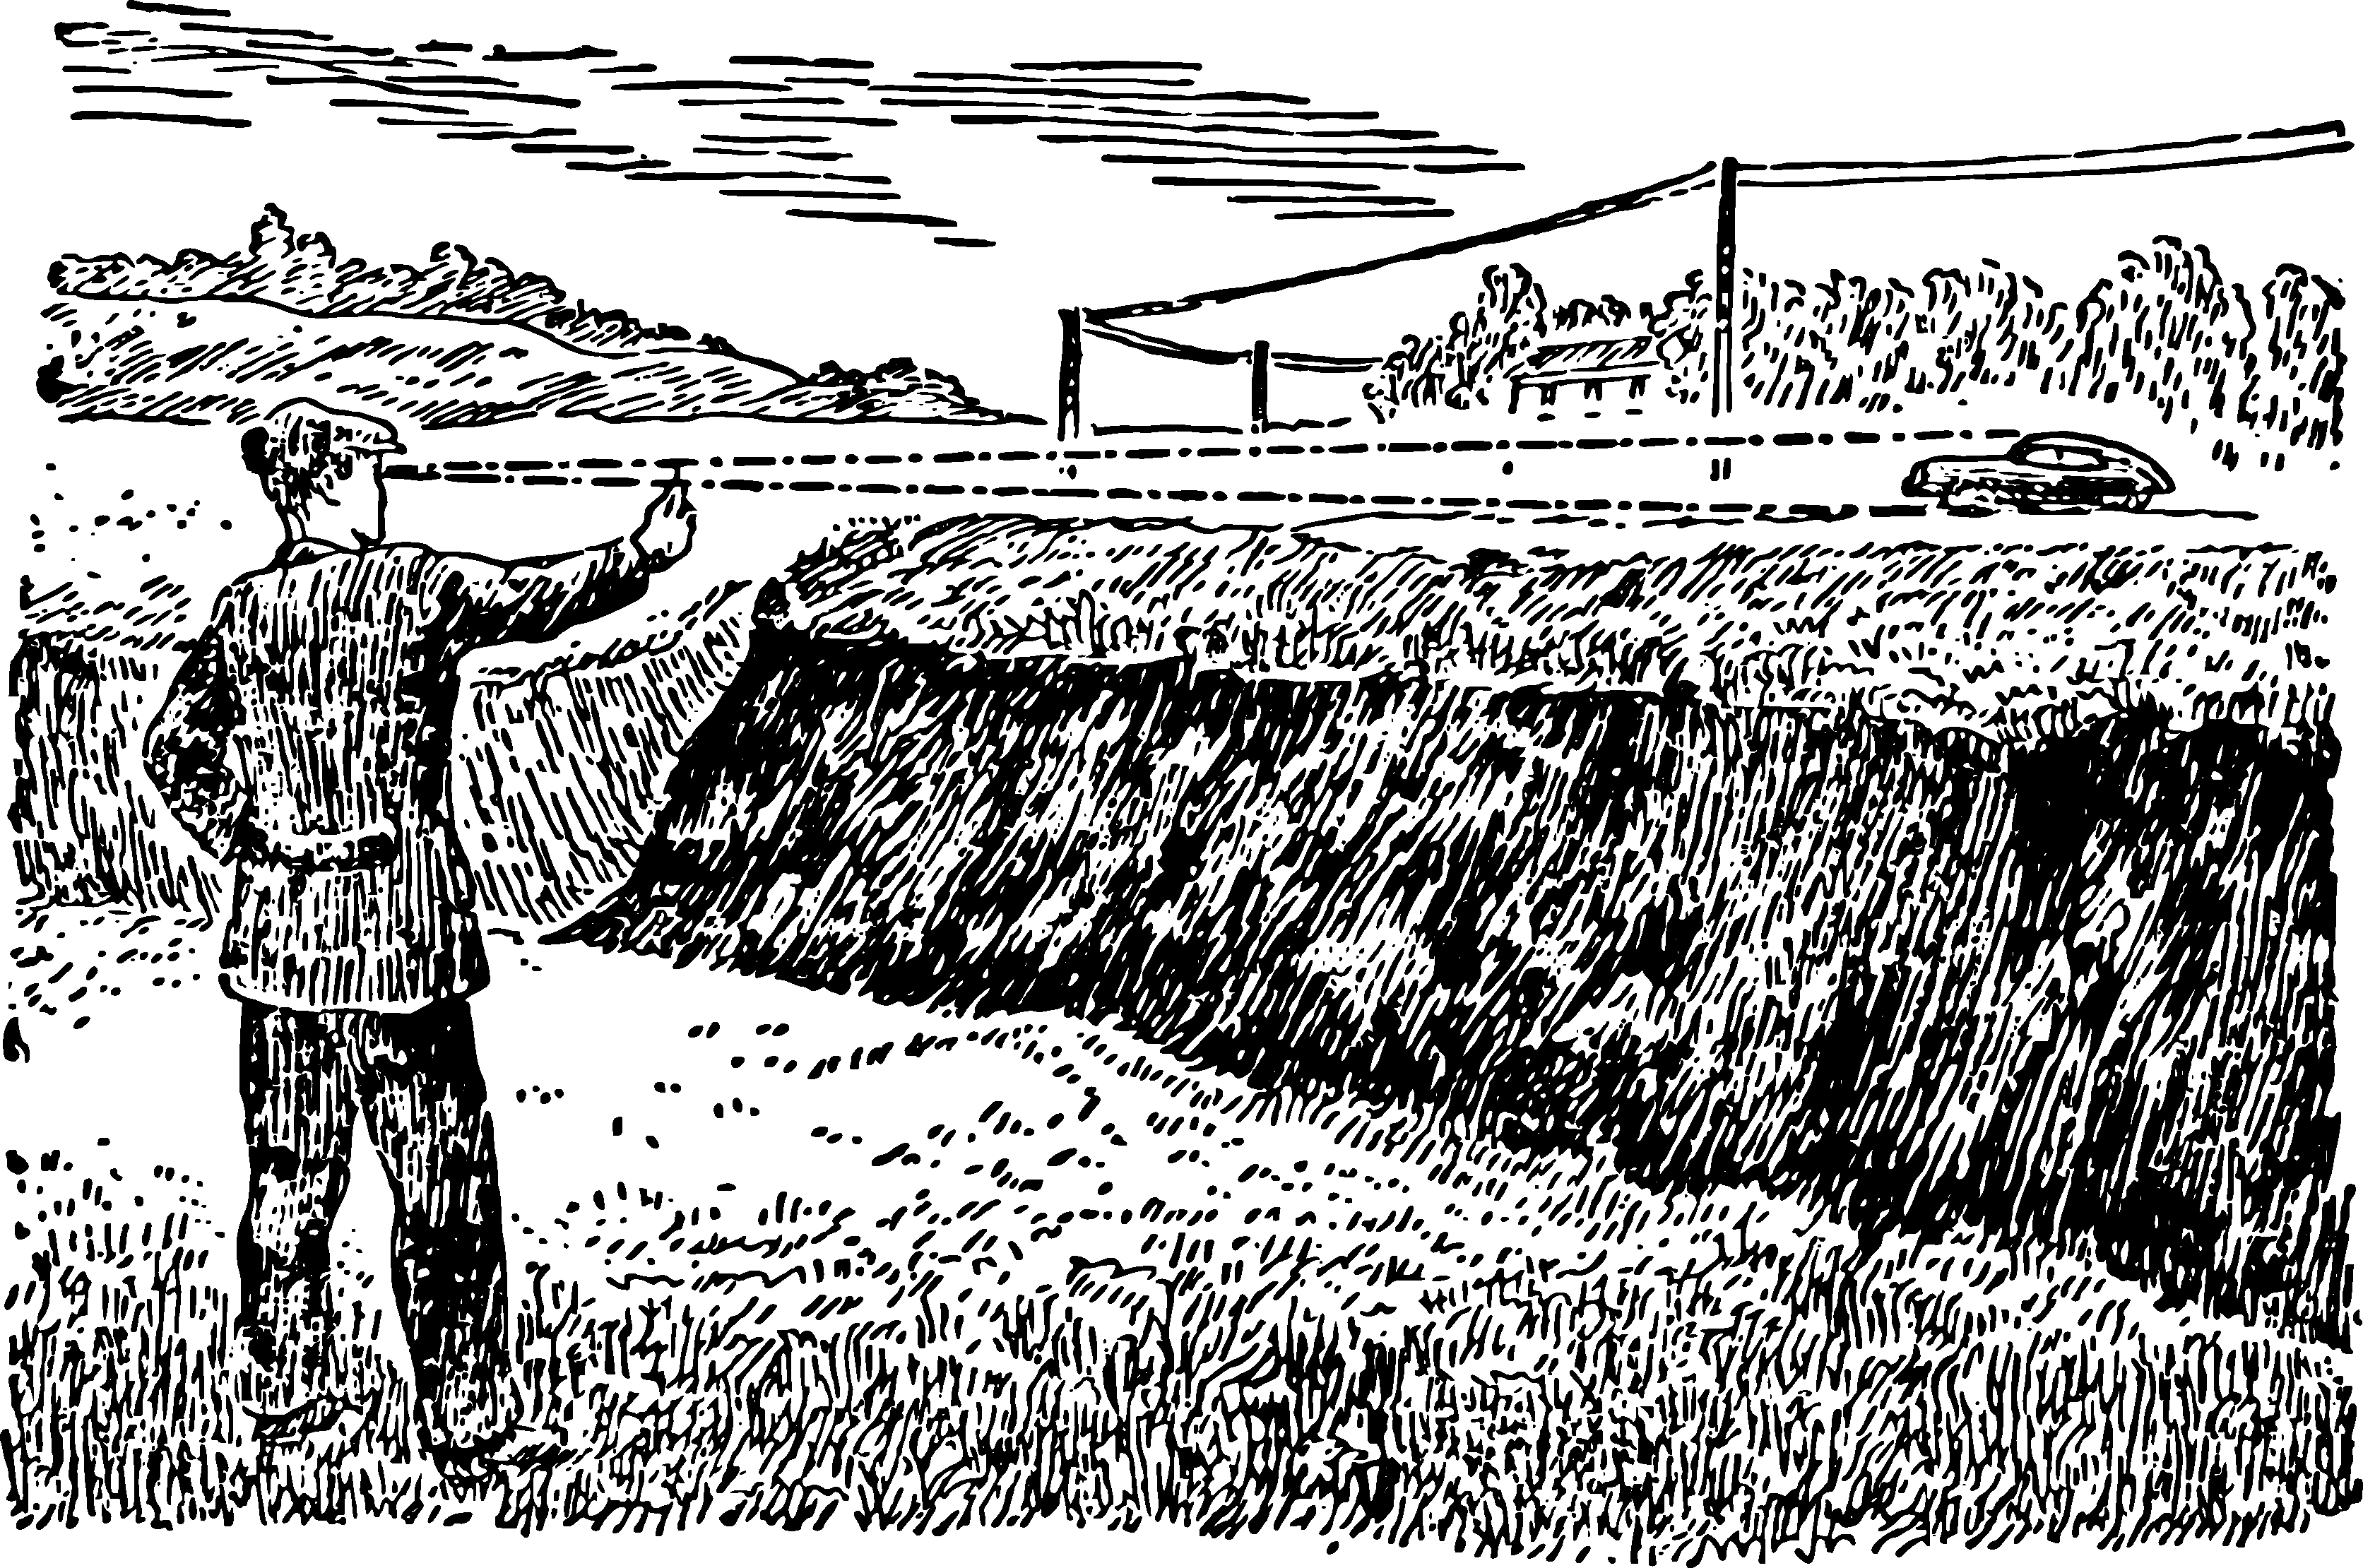
\includegraphics[width=\textwidth]{figures/ch-02/fig-038.pdf}
\sidecaption{The use of a rangefinder match to determine inaccessible distances.\label{fig-038}}
\end{figure}

You can easily verify the correctness of the proportion:
\begin{equation*}%
\frac{\text{desired distance}}{\begin{array}{c}\text{distance from the eye}\\ \text{to the matchstick}\end{array}} = \frac{\text{average height of a person}}{\begin{array}{c}\text{measured part}\\ \text{of the matchstick}\end{array}}
\end{equation*}
From here, it's easy to calculate the desired distance. For example, if the distance to the matchstick is \SI{60}{\centi\meter}, the height of the person is \SI{1.7}{\meter}, and the measured part of the matchstick is \SI{12}{\milli\meter}, then the determined distance would be:
\begin{equation*}%
60 \cdot \frac{1700}{12} = \SI{8500}{\centi\meter} = \SI{85}{\meter}.
\end{equation*}
To gain some skill in using this rangefinder, measure the height of someone from your group and, asking them to move away a certain distance, try to determine how many steps they took away from you.

With the same method, you can determine the distance to a rider (average height \SI{2.2}{\meter}), a cyclist (wheel diameter \SI{75}{\centi\meter}), a telegraph pole along the railway track (height \SI{8}{\meter}), vertical distance between adjacent insulators (\SI{90}{\centi\meter}), to a train, a brick house, and similar objects whose dimensions can be estimated with sufficient accuracy. There can be quite a few such cases during excursions.

\begin{marginfigure}%[-2cm]%[h!]
\centering
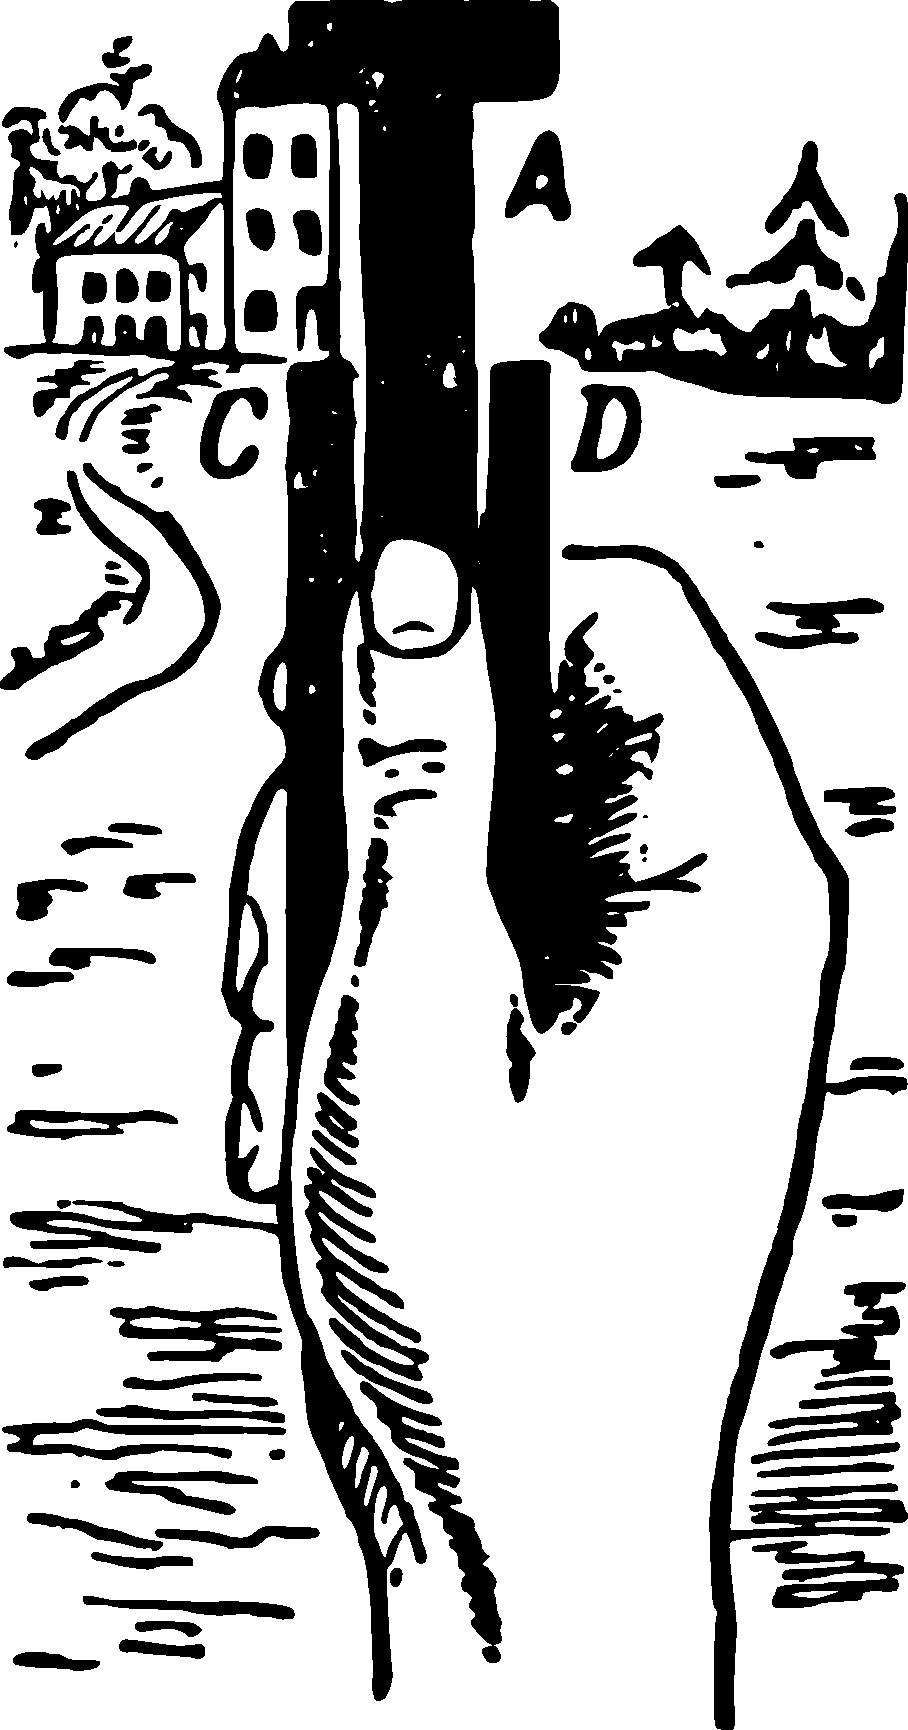
\includegraphics[width=0.8\textwidth]{figures/ch-02/fig-039.pdf}
\sidecaption{The retractable rangefinder in action.\label{fig-039}}
\end{marginfigure}

For those skilled in crafting, making a more convenient device of the same type, intended for estimating distances based on the size of a distant human figure, won't be much trouble.

\begin{marginfigure}%[-2cm]%[h!]
\centering
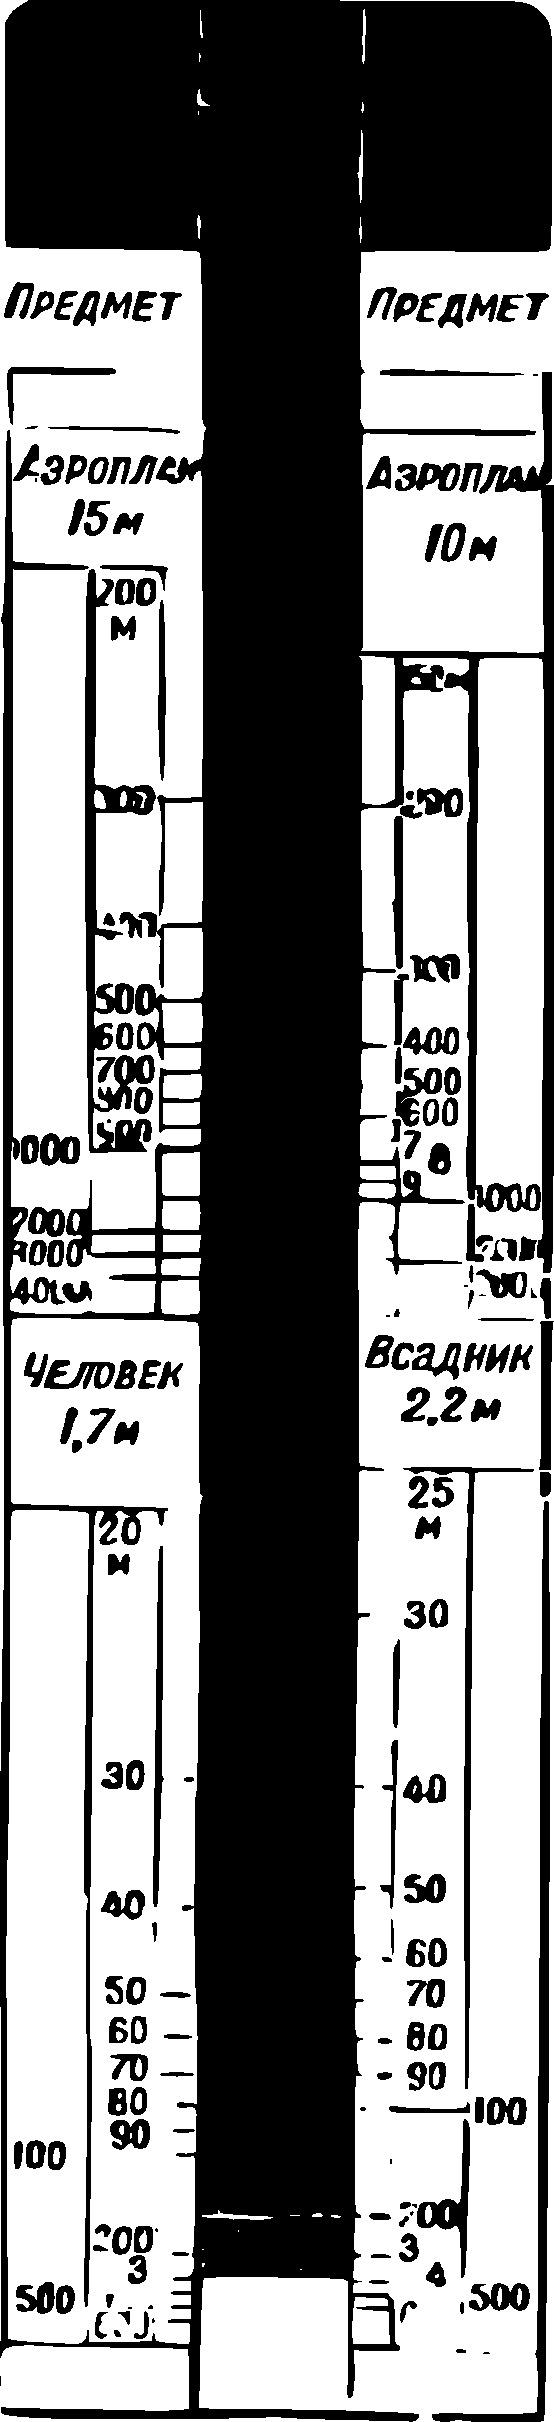
\includegraphics[width=0.6\textwidth]{figures/ch-02/fig-040.pdf}
\sidecaption{The design of the retractable rangefinder.\label{fig-040}}
\end{marginfigure}

The device is clear in \figr{fig-039} and \figr{fig-040}. The observed object is placed precisely in the gap $A$, formed when the extension part of the device is raised. The size of the gap can be conveniently determined by the divisions on the part $C$ and $D$ of the board. To avoid the need for any calculations, you can directly mark on strip $C$ the distances corresponding to the divisions if the observed object is a human figure (the device for measuring the distance of the outstretched arm). On the right strip $D$, you can mark distances, pre-calculated for cases where a rider is observed (\SI{2.2}{\meter}). For telegraph poles (height \SI{8}{\meter}), planes with a wingspan of \SI{15}{\meter}, and other larger objects, you can use the upper, free parts of strips $C$ and $D.$ Then the device will look like the one presented in \figr{fig-040}.





Of course, the accuracy of such distance estimation is low. It's just an estimate, not a measurement. In the example discussed earlier, where the distance to the human figure was estimated at \SI{85}{\meter}, an error of \SI{1}{\milli\meter} in measuring the matchstick portion would result in a deviation of \SI{7}{\meter} (1/12 out of 85). But if the person stood four times farther away, and we measured only \SI{3}{\milli\meter} on the matchstick, then an error of even 1/2 mm would cause a change in the result by \SI{57}{\meter}. Therefore, our example is reliable only for relatively short distances -- in the range of 100--200 m. When estimating larger distances, it's necessary to choose larger objects.


\section{The energy of the river}
\label{sec-2.6}

\begin{quote}
\emph{You know the edge where everything breathes abundance,\\
Where rivers flow purer than silver, \\
Where the steppe breeze sways the feather grass, \\
Where villages are nestled in cherry orchards.}\\[-10pt]
\flushright{\emph{A.K. Tolstoy}}
\end{quote}


A river, the length of which is no more than 100 km, is considered small. Do you know how many such small rivers there are in the USSR? A lot - 48 thousand!

If these rivers were stretched into a single line, it would result in a ribbon \SI{13800000}{\kilo\meter} long. With such a ribbon, you could encircle the Earth at the equator thirty times (the length of the equator is approximately \SI{40009}{\kilo\meter}).

The flow of these rivers is leisurely, but it conceals an inexhaustible supply of energy within it. Specialists believe that if the hidden potential of all the small rivers flowing through our homeland were combined, an impressive number would be obtained -- 34 million kilowatts! This gifted energy needs to be widely utilised for electrifying the economy of settlements located near rivers.

\begin{quote}
\emph{Let the river flow freely,\\
If the plan says so,\\
A dam with a stone ridge across all depths\\
Will block the way forever.}\\[-10pt]
\flushright{\emph{S. Shchipachev}}
\end{quote}

You know that this is achieved through hydroelectric power stations (HPS), and you can show a lot of initiative and provide real assistance in preparing for the construction of small HPS. Indeed, the builders of HPS will be interested in everything related to the river regime: its width and flow rate (``water flow''), the area of the cross-section of the riverbed (``active section''), and what water head the banks allow. And all this can be measured with available means and represents a relatively simple geometric problem.

We will now proceed to solving this problem.

But first, let's present here a practical advice from specialists, engineers V. Yarosh and I. Fedorov, regarding the selection of a suitable location on the river for the construction of a future dam.

They recommend building a small hydroelectric power station with a capacity of 15-20 kilowatts ``no further than 5 km from the village.''

``The dam of an HPS should be built no closer than 10-15 km and not farther than 20-40 km from the source of the river because moving away from the source entails the costly reinforcement of the dam, which is caused by a large influx of water. If the dam is located closer than 10-15 km from the source, due to the small water flow and insufficient head, the hydroelectric power station will not be able to provide the necessary power. The chosen stretch of the river should not be abundant in great depths, which also increases the cost of construction, requiring a heavy foundation.''

\section{The Flow Rate}
\label{sec-2.7}
\begin{quote}
\emph{Between village and mountain grove,\\
Winds a river like a bright ribbon.}\\[-10pt]
\flushright{\emph{A. Fet}}
\end{quote}

How much water flows in such a river in a day? It's easy to calculate if you first measure the speed of the water flow in the river. The measurement is performed by two people. One person holds a watch, the other holds some noticeable float, for example, a half-empty bottle with a flag. They choose a straight section of the river and place two stakes $A$ and $B$ along the bank at a distance, for example, \SI{10}{\meter} from each other (see \figr{fig-041}).

\begin{figure}[h!]
\centering
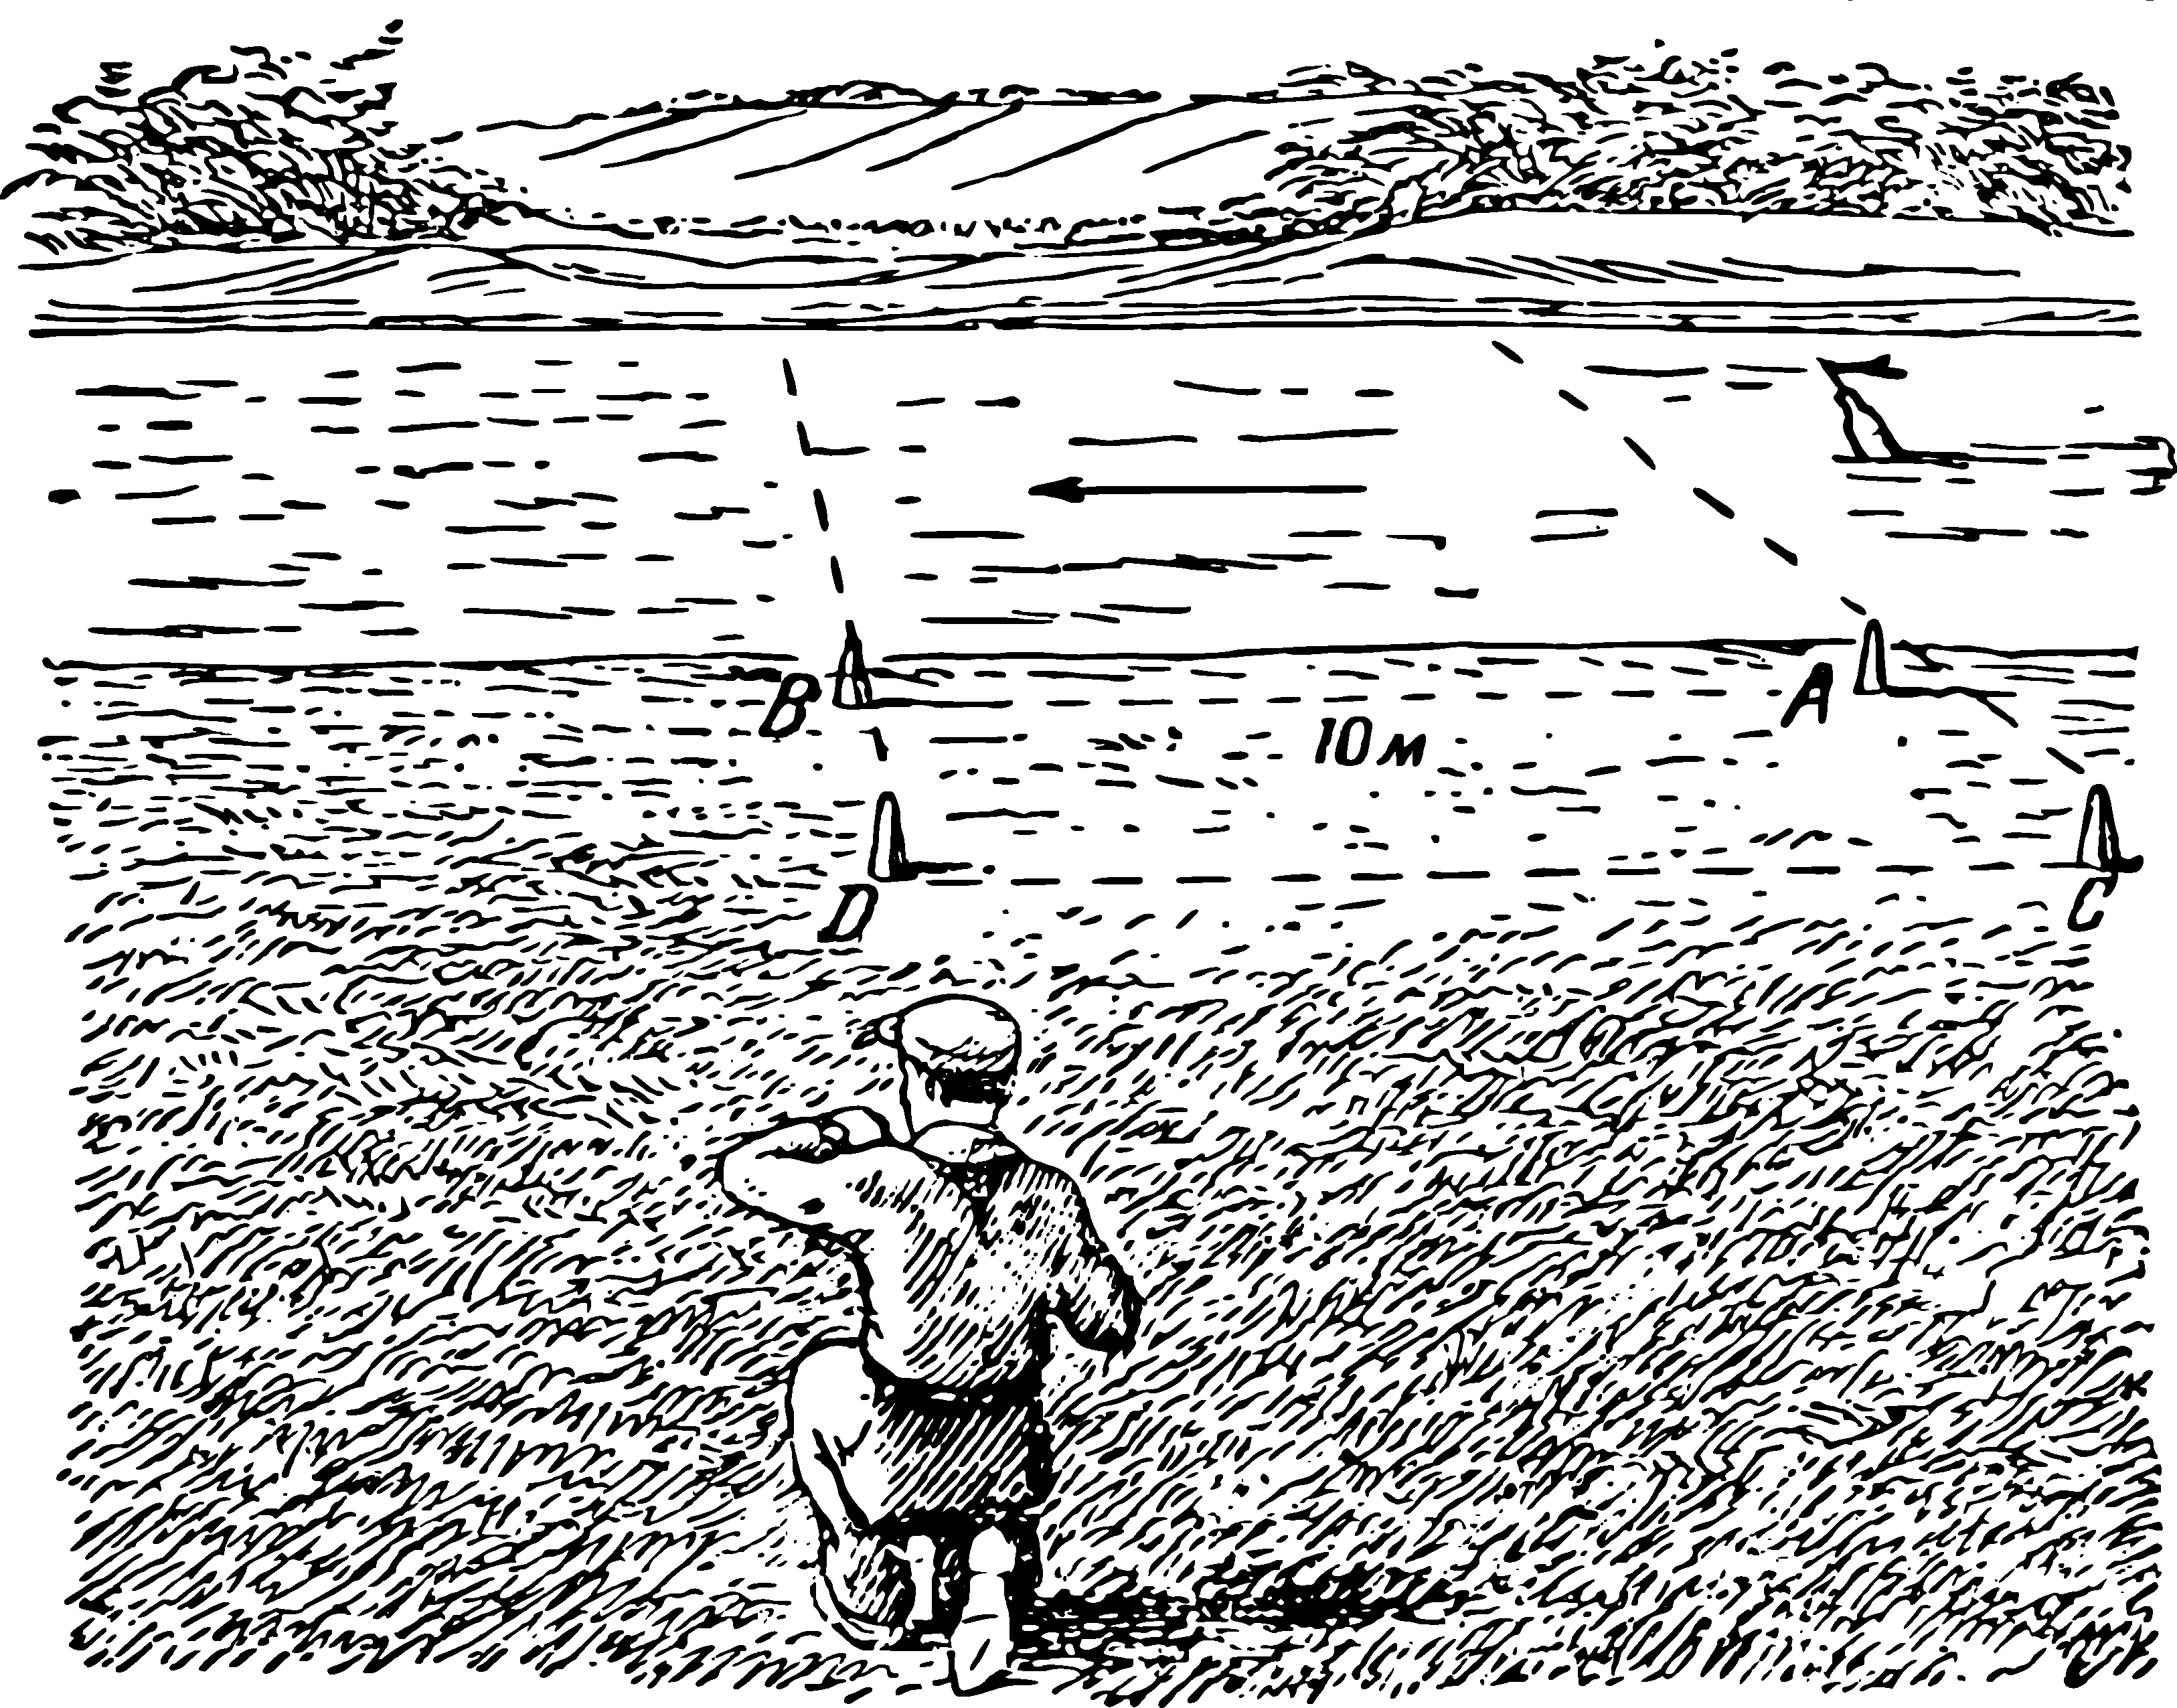
\includegraphics[width=0.9\textwidth]{figures/ch-02/fig-041.pdf}
\sidecaption{Measurement of the river flow velocity.\label{fig-041}}
\end{figure}

Two more stakes $C$ and $D$ are placed on lines perpendicular to $AB$. One of the participants in the measurement with the watch stands behind stake $D$. The other, with the float, goes a bit upstream of stake $A$, throws the float into the water, and then stands behind stake $C$. Both observers look along the directions $CA$ and $DB$ towards the water surface. At the moment when the float crosses the extension of the line $CA$, the first observer waves his hand. Upon this signal, the second observer starts the timer for the first time and then again when the float crosses the direction of $DB$.

Let's assume that the time difference is 20 seconds.

Then the speed of the water flow in the river is:
\begin{equation*}%
\frac{10}{20} = \SI{0.5}{\meter\per\second}.
\end{equation*}
Usually, the measurement is repeated about ten times\sidenote{Instead of throwing one float ten times, you can immediately throw 10 floats at some distance from each other.}, throwing the float into different points on the river surface. Then the obtained numbers are summed up and divided by the number of measurements. This gives the average speed of the surface layer of the river.

Deeper layers flow slower, and the average speed of the entire flow is approximately 4/5 times the surface speed. In our case, therefore, it's \SI{0.4}{\meter\per\second}.

You can determine the surface speed by another -- albeit less reliable -- method.

Sit in a boat and paddle \SI{1}{\kilo\meter} (measured along the shore) against the current, and then back -- with the current, trying to paddle with the same force all the time.

Let's say you paddled these \SI{1000}{\meter} against the current in 18 minutes, and with the current in 6 minutes. Denoting the desired speed of the river current as $x$, and the speed of your movement in still water as $y$, you form the equations:
\begin{equation*}%
\frac{1000}{y - x} = 18, \qand \frac{1000}{y + x} = 6.
\end{equation*}
Rearranging we get:
\begin{equation*}%
y + x = \frac{1000}{6}, \qand y - x = \frac{1000}{18}.
\end{equation*}
Solving for $x$, we get $2x = 110$, and $x = 55$. The speed of the water flow on the surface is 55 m per minute, and therefore, the average speed is about 5/6 \si{\meter\per\second}.


\section{How Much Water Flows In The River?}


To measure the amount of water flowing in a river, you can always determine the speed at which the water flows. The more challenging part of the preparatory work needed to calculate the quantity of flowing water is to determine the cross-sectional area of the water. To find the magnitude of this area, known as the ``live cross-section'' of the river, you need to make a drawing of this section. Such work is done as follows.

\textbf{First Method:} At the point where you measured the width of the river, you drive a stake into the ground on both banks, right at the water's edge. Then, with a companion, you get into a boat and row from one stake to the other, trying to keep a straight line connecting the stakes. An inexperienced rower will not be able to handle such a task, especially in a river with a fast current. Your companion must be a skilled rower; besides, a third participant in the work should stand on the bank, ensuring that the boat stays on the correct course and giving the rower signals indicating which way to turn when necessary. During the first crossing of the river, you only need to count how many strokes of the oars it took and from there figure out how many strokes move the boat 5 or 10 meters. Then, for the second crossing, armed with a sufficiently long rake with markings on it, you plunge the rake vertically to the bottom every 5-10 meters (measured by the number of oar strokes) and record the depth of the river at that point.

This method can only measure the live cross-section of a small river; for a wide, multi-water river, more complex methods are needed, which are performed by specialists. An amateur must choose a task that suits their modest measuring means.

\textbf{Second Method:} On a narrow and shallow river, you don't need a boat.

Between the stakes, you stretch a cord perpendicular to the current with marks or knots made on it every 1 or 2 meters, and by lowering a ruler to the bottom at each knot, you measure the depth of the riverbed. When all measurements are done, you first draw a millimeter paper or a grid paper sketch of the cross-section profile of the river. You will get a figure similar to the one shown in \figr{fig-042}. It is quite easy to determine the area of this figure since it can be divided into a series of trapezoids (where both bases and the height are known) and two side triangles, also with known base and height. If the scale of the drawing is 1:100, then the result will be obtained directly in square meters.

\begin{figure}[h!]
\centering
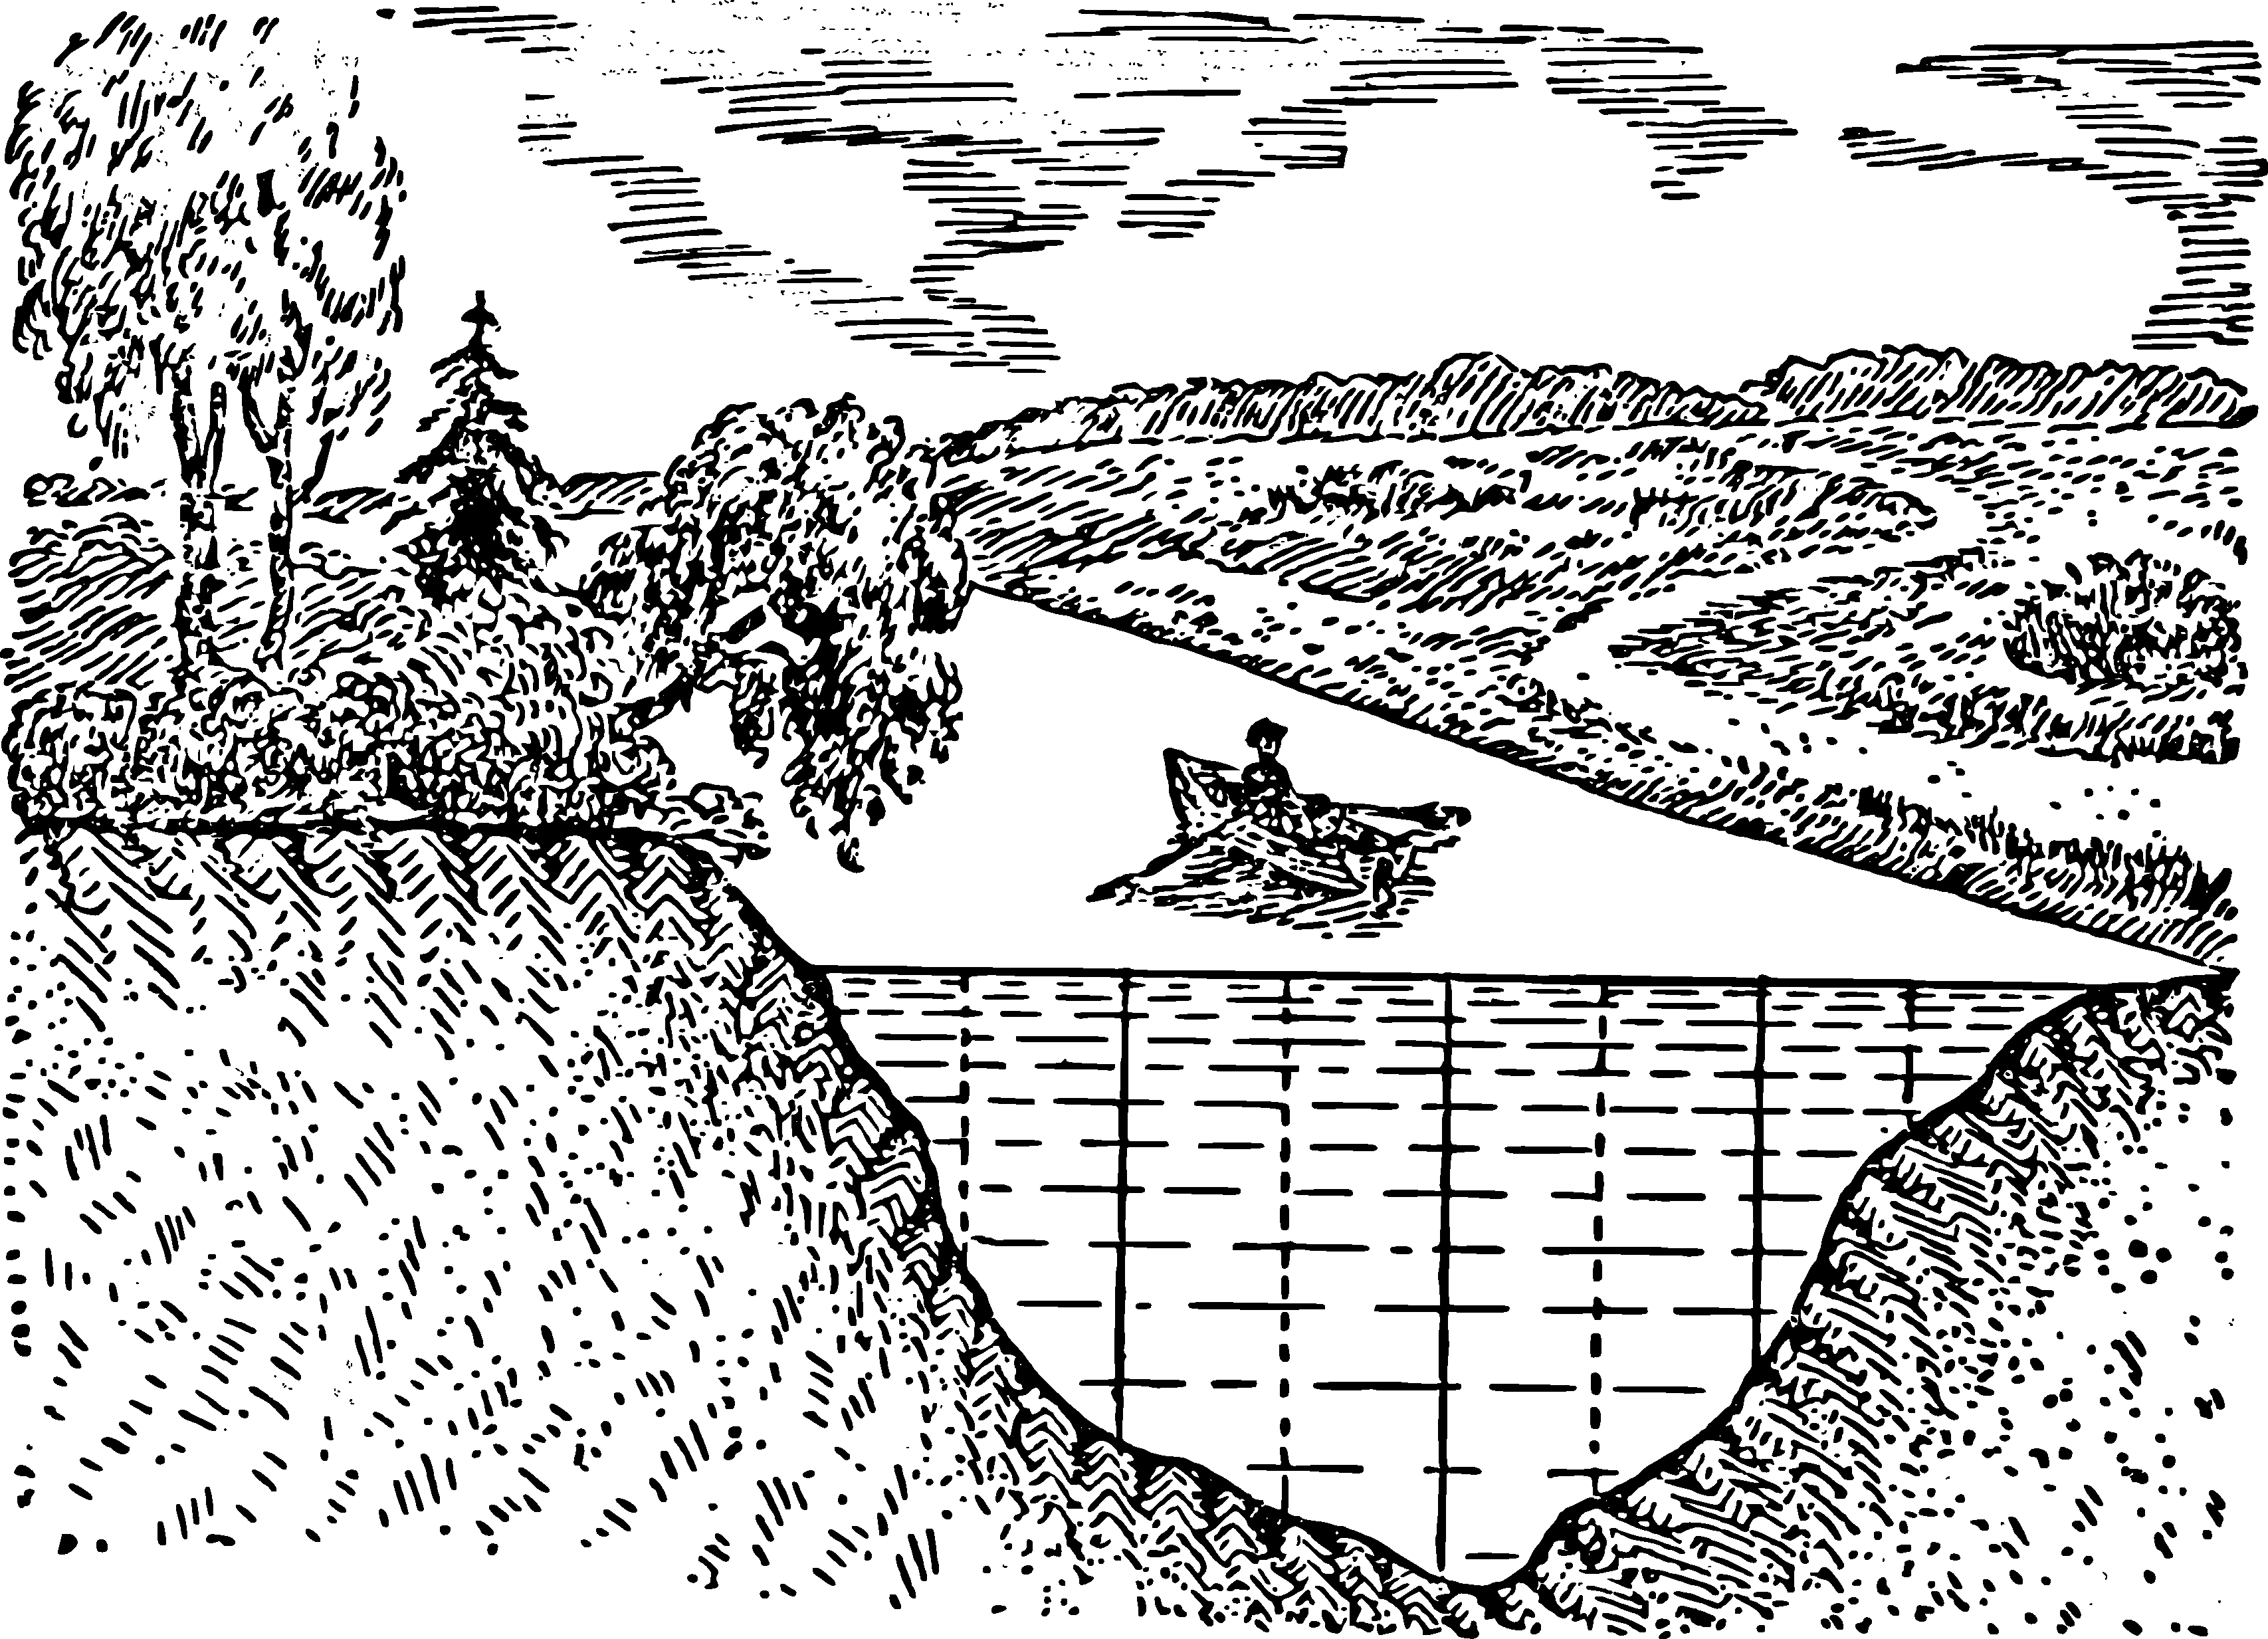
\includegraphics[width=0.9\textwidth]{figures/ch-02/fig-042.pdf}
\sidecaption{``Live Cross-Section'' of a River.\label{fig-042}}
\end{figure}

Now you have all the data needed to calculate the amount of flowing water. Obviously, through the live cross-section of the river, a volume of water equal to the volume of a prism is passing every second, where the cross-section serves as the base and the average second-by-second flow rate serves as the height. For example, if the average flow rate of water in the river is 0.4 meters per second, and the area of the live cross-section is, let's say, 3.5 square meters, then every second, through this section, there will be a transfer of

3.5 * 0.4 = 1.4 cubic meters of water,

or the same amount in tons. This amounts to 1.4 x 3600 = 5040 cubic meters per hour, and 5040 x 24 = 120960 cubic meters per day, which is over a hundred thousand cubic meters. And yet, a river with a wetted cross-section of 3.5 square meters is a small river; it could be, for example, 3.5 meters wide and 1 meter deep at a fordable point. But even it contains energy capable of transforming into mighty electricity. So how much water flows per day in a river like the Neva, through which 3300 cubic meters of water pass every second through its wetted cross-section! This is the 'average flow rate' of water in the Neva at Leningrad. The 'average flow rate' of water in the Dnieper at Kiev is 700 cubic meters.

Young explorers and future dam builders also need to determine the maximum head the banks can allow, i.e., the difference in water levels that the dam can create (Fig. 43). To do this, stakes are driven into the banks 5-10 meters away from the water, as usual, along a line perpendicular to the river's current. Then, moving along this line, small stakes are placed at points of characteristic bends in the banks (Fig. 44). Using rulers with markings, the elevation of one stake above the other and the distances between them are measured. Based on the measurement results, a profile of the banks is drawn similar to the profile of the riverbed. The bank profile can indicate the magnitude of the allowable head.

Suppose the water level can be raised by the dam by 2.5 meters. In this case, you can estimate the potential power of your future hydroelectric power plant.

For this, energy experts recommend multiplying 1.4 (the second-by-second flow rate of the river) by 2.5 (the water level height) and by 6 (the coefficient, which varies depending on energy losses in machines). The result will be in kilowatts. Thus,

1.4 x 2.5 x 6 = 21 kilowatts.

Since the river levels, and consequently the flow rates, vary throughout the year, it is necessary to calculate the value of the flow rate that is characteristic of the river for most of the year."

%\begin{center}
%
\includegraphics[width=0.3\textwidth]{figures/ch-02/fig-ch-02-tail.pdf}
%\end{center}



















% !TEX root = perelman-geometry.tex
%!TEX TS-program = pdflatex
%!TEX encoding = UTF-8 Unicode

\setchapterpreamble[o]{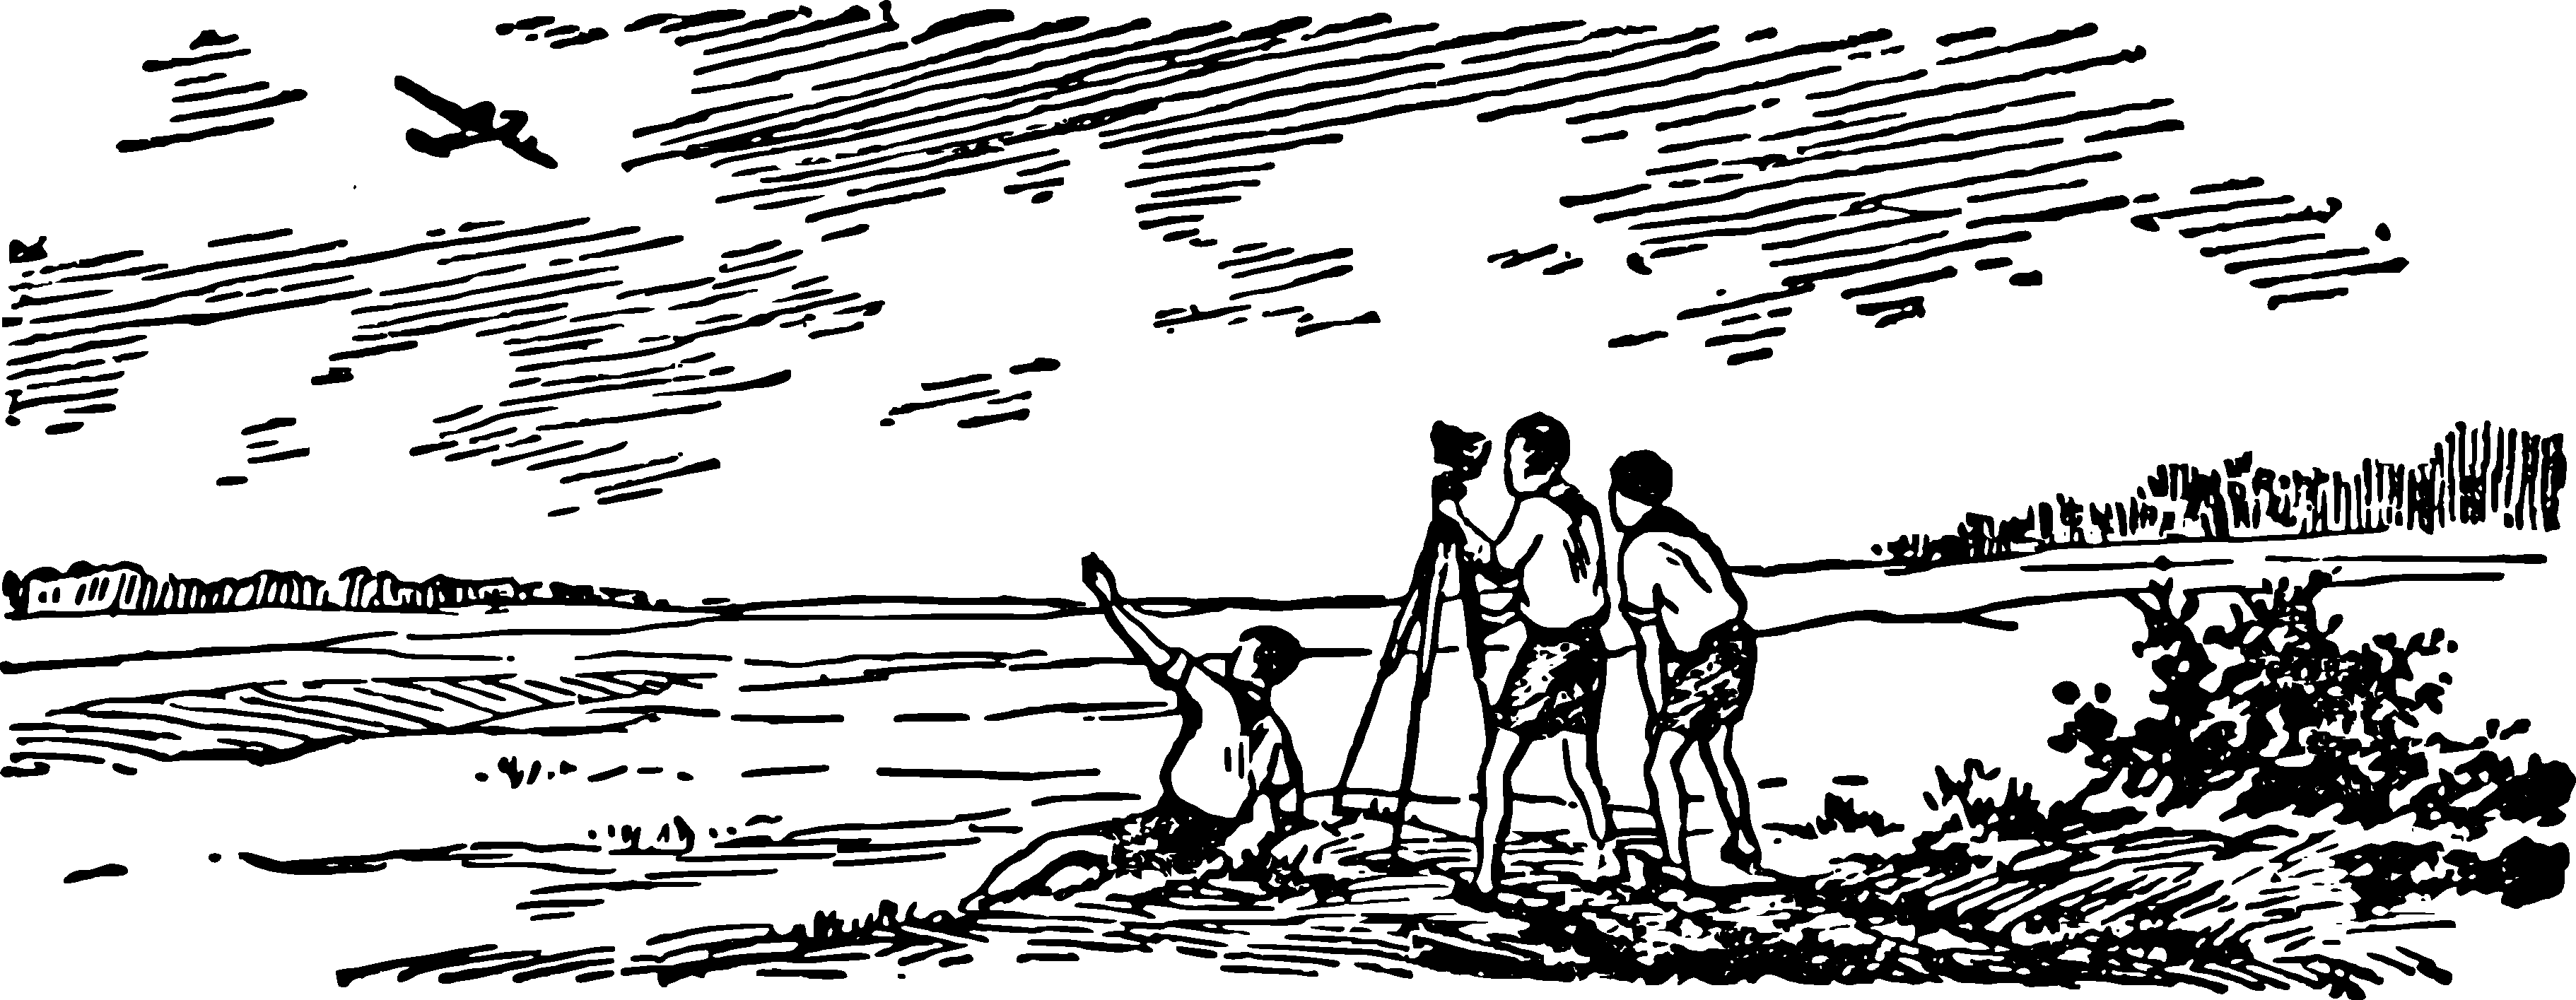
\includegraphics[width=1.2\textwidth]{figures/ch-03/fig-ch-03-head.pdf}\bigskip}

\chapter{Geometry In The Open Field}
\label{ch-03}

\section{Visible sizes of the Moon}
\label{sec-3.1}


What size does the full moon in the sky seem to you? Different people give quite different answers to this question.

Estimates like ``the size of a plate,'' ``the size of an apple,'' ``the size of a human face,'' and so on, are extremely vague, indefinite, indicating only that those answering do not understand the essence of the question.

The correct answer to such an apparently ordinary question can only be given by someone who clearly understands what exactly needs to be understood by the ``apparent'' or ``visible'' size of an object. Few suspect that here we are referring to the magnitude of a certain angle -- precisely the angle formed by two straight lines drawn to our eye from the extreme points of the object under consideration; this angle is called the ``angle of view'' or ``angular size of the object'' (\figr{fig-061}). 

\begin{figure}[h!]
\centering
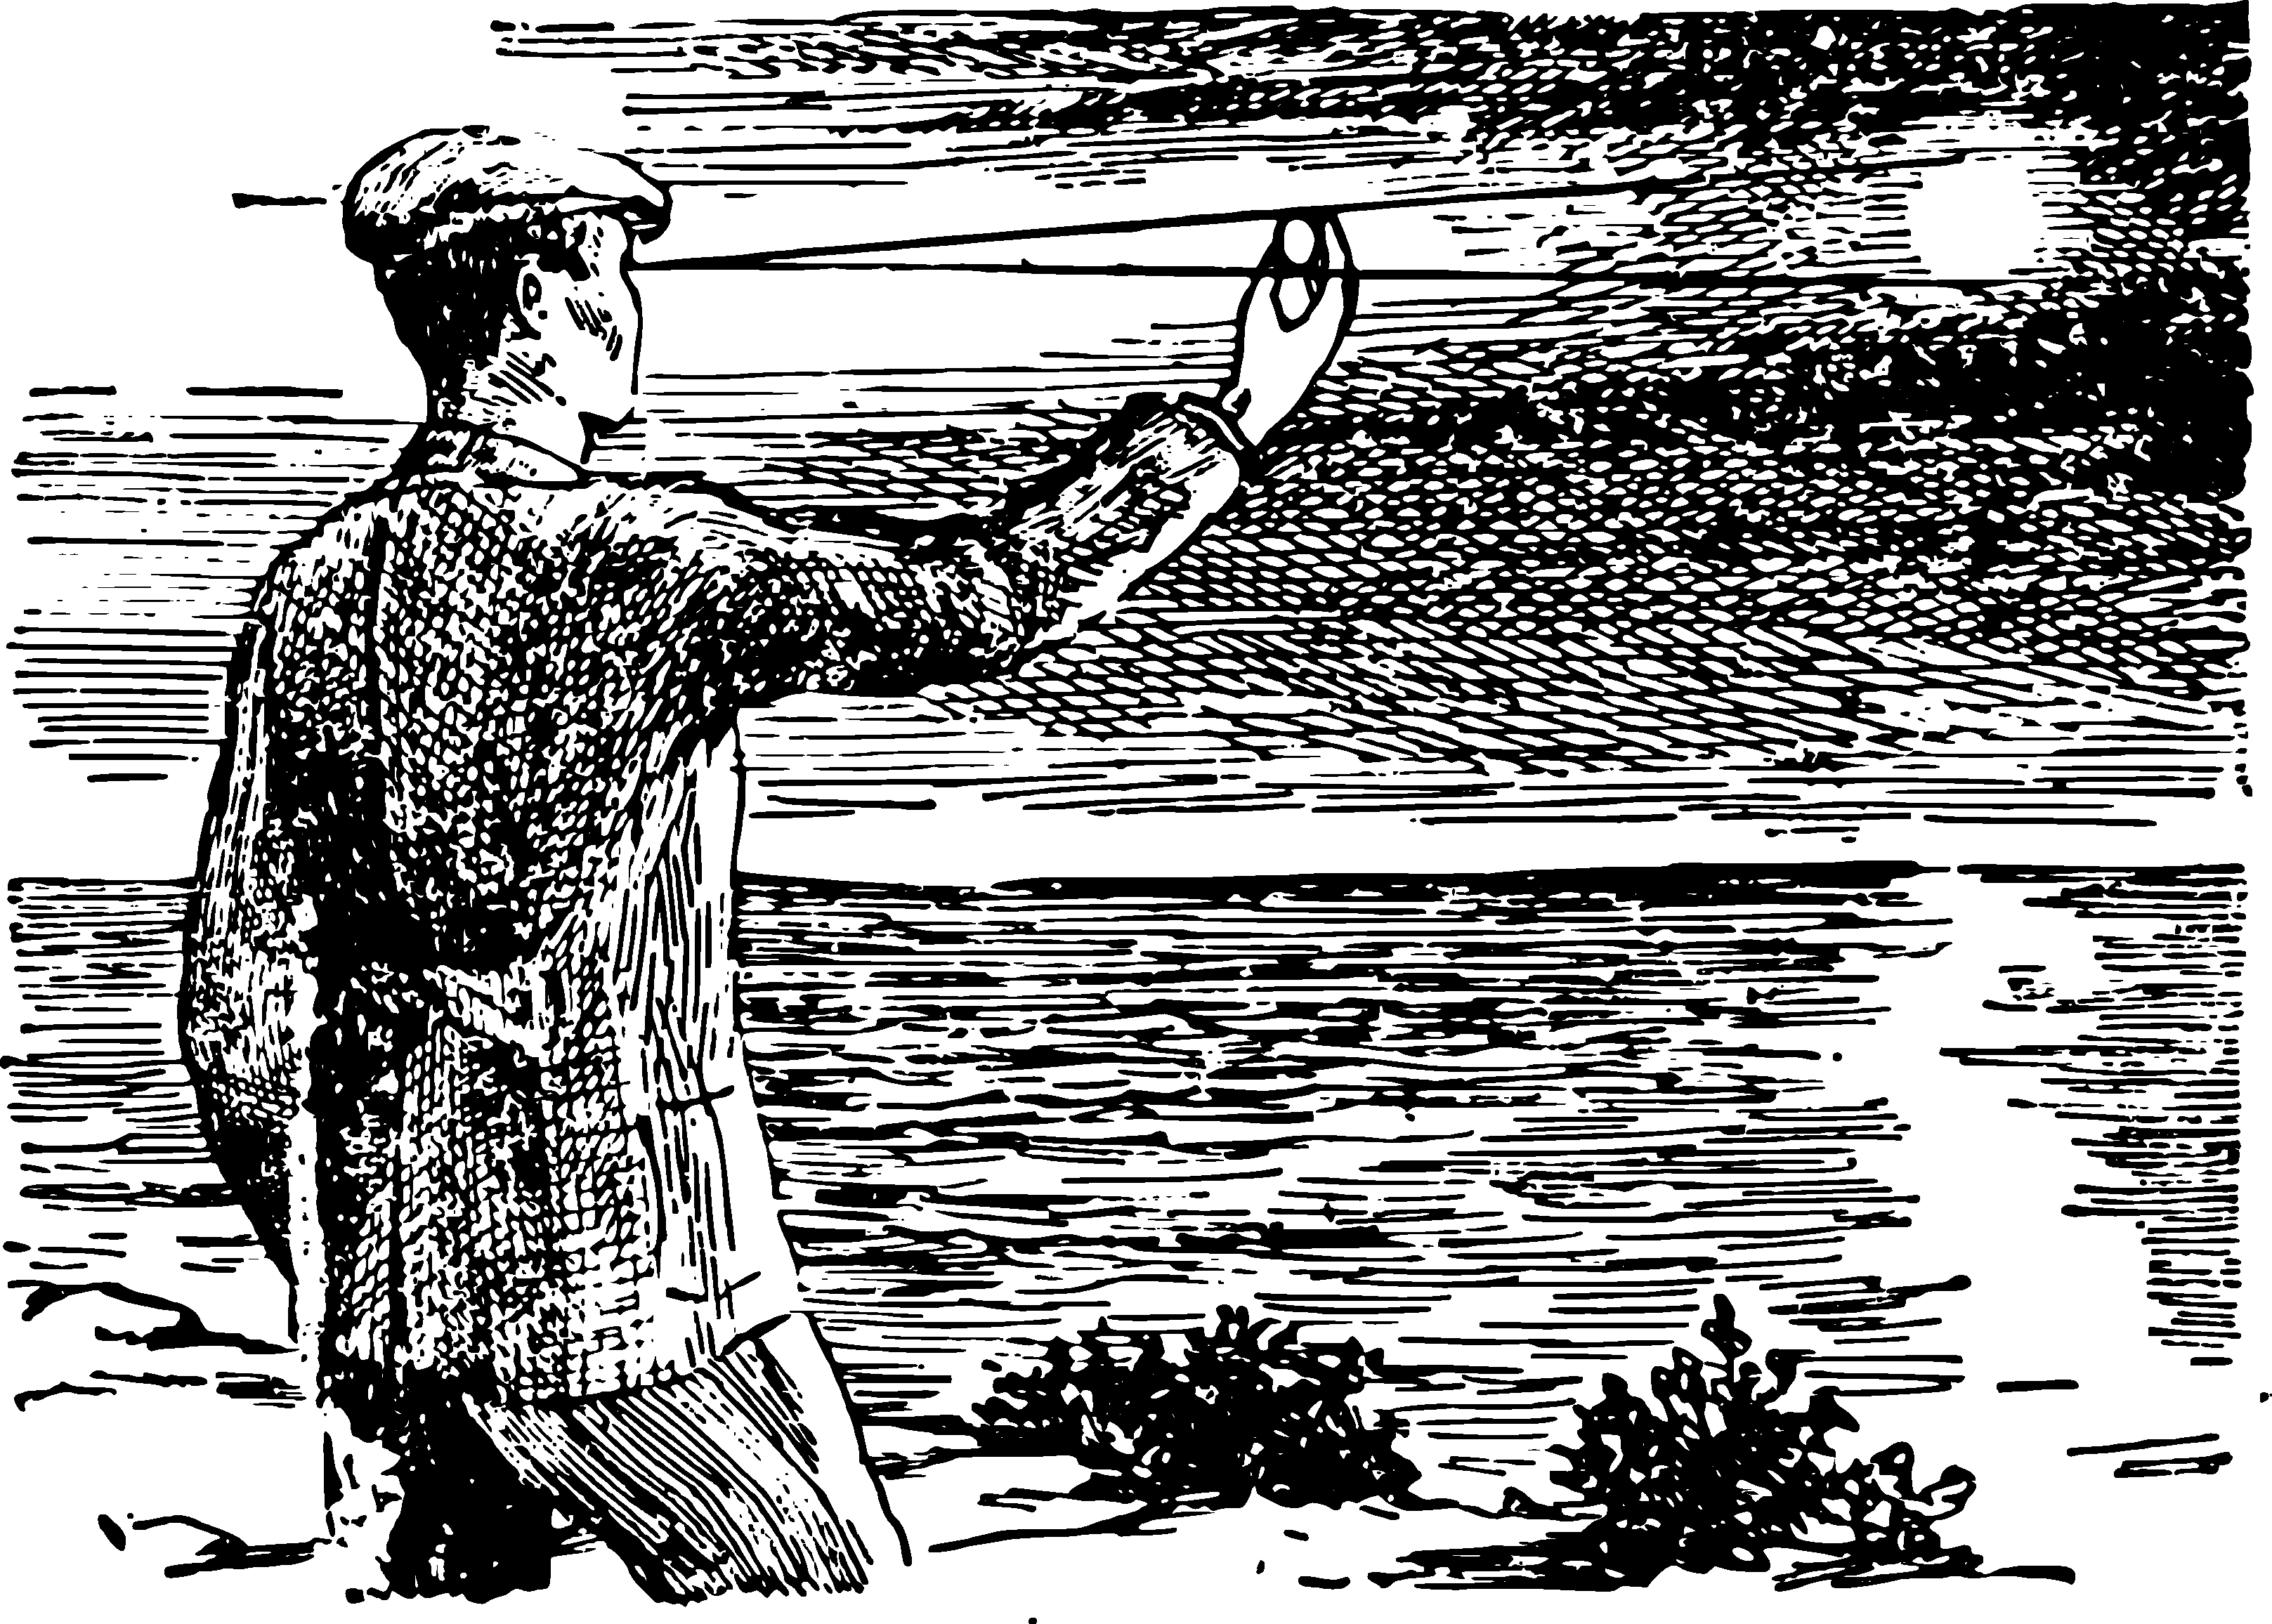
\includegraphics[width=0.9\textwidth]{figures/ch-03/fig-061.pdf}
\sidecaption{What is the angle of view or angular size of the object.\label{fig-061}}
\end{figure}

And when the apparent size of the Moon in the sky is assessed by comparing it with the sizes of a plate, an apple, and so forth, such answers are either completely meaningless or should imply that the Moon is visible in the sky at the same angle as the plate or apple. But such an indication alone is still insufficient: after all, we see a plate or an apple under different angles depending on their distance: up close -- under larger angles, far away -- under smaller ones. To introduce clarity, it is necessary to specify from what distance the plate or apple is being observed. Comparing the sizes of distant objects with the sizes of others, the distance of which is not indicated, is a very common literary technique employed by even first-rate writers. It creates a certain impression due to its closeness to the familiar psychology of most people, but it does not produce a clear image\ldots{} Here's an example from Shakespeare's \emph{King Lear}; it describes (by Edgar) the view from a high cliff by the sea:
\begin{quote}
\emph{How terrifying! How my head spins!\\
How low to cast my gaze\ldots{}\\
The rooks and crows that flutter there in the air at mid-distance,\\ Seem barely as large as flies. Halfway down Hangs a man gathering seaweed\dots{} \\
What a dreadful trade! He seems to me no bigger than his head.\\
The fishermen walking along the shore -- like mice;\\
and that tall ship at anchor has shrunk to the size of its boat;\\ its boat -- a floating dot, As if too small for sight\dots{}}
\end{quote}
These comparisons would provide a clear idea of distance if accompanied by indications of the degree of remoteness of the objects being compared (mice, the human head, crows, boat \dots{}). Similarly, when comparing the size of the moon with that of a plate or apples, indications of how far these everyday objects should be from the eye are necessary.

This distance turns out to be much greater than commonly thought. Holding an apple at arm's length, you not only obscure the Moon but also a significant portion of the sky. Suspend the apple on a string and gradually move away from it until it just covers the full lunar disk: in this position, the apple and the Moon will have the same apparent size for you. By measuring the distance from your eye to the apple, you will find that it is approximately 10 meters. This is how far you would need to move the apple away from you for it to truly seem to be the same size as the Moon in the sky! A plate, on the other hand, would need to be moved about 80 meters away from you, or about fifty steps.

What is said may seem unbelievable to anyone hearing it for the first time; however, it is indisputable and follows from the fact that we perceive the Moon at an angle of only \emph{half a degree}. We rarely have to estimate angles in our everyday lives, and therefore most people have a very vague idea of the magnitude of an angle with a small number of degrees, such as an angle of \ang{1}, \ang{29}, or \ang{59} (not to mention surveyors, draftsmen, and other specialists accustomed to practically measuring angles). We only estimate large angles more or less reasonably, especially if we manage to compare them with angles familiar to us between the hands of a clock; everyone, of course, is familiar with angles of \ang{90}, \ang{60}, \ang{30}, \ang{120}, \ang{150}, which we are so accustomed to seeing on a dial (at 8 o'clock, 2 o'clock, 1 o'clock, 4 o'clock, 5 o'clock) that even without distinguishing the numbers, we guess the time based on the size of the angle between the hands. But we usually see small and individual objects at much smaller angles and therefore completely lack the ability to even approximately estimate angles of view.


\section{Angle of View}
\label{sec-3.2}

To provide a concrete example of a one-degree angle, let's calculate how far an average-height person (1.7 meters) should move away from us to appear at such an angle. Translating the problem into the language of geometry, let's say we need to calculate the radius of a circle, the arc of which at \ang{1} has a length of 1.7 meters (strictly speaking, not an arc, but a chord, but for small angles, the difference between the lengths of the arc and the chord is negligible). We reason as follows: if the arc at \ang{1} equals 1.7 meters, then the full circumference containing \ang{360} will have a length of $1.7 \times 360 = \SI{610}{\meter}$, and the radius will be $1/2\pi$ the length of the circumference; if we take the value of $\pi$ as approximately 22/7, then the radius will be equal to
\begin{equation*}%
 \frac{610}{44/7} \approx \SI{98}{\meter}.
\end{equation*}
\begin{figure}[h!]
\centering
\includegraphics[width=0.9\textwidth]{figures/ch-03/fig-062.pdf}
\sidecaption{The human figure is visible from a distance of about hundred meters at an angle of \ang{1}.\label{fig-062}}
\end{figure}
So, a person appears at an angle of \ang{1} if they are approximately at a distance of 100 meters from us (\figr{fig-062}). If they move twice as far away -- to 200 meters -- they will be seen at an angle of half a degree; if they approach to a distance of 50 meters, the angle of view will increase to \ang{2}, and so on. It is also easy to calculate that a stick of 1 meter in length should appear to us at an angle of 1° at a distance of $360/(44/7) = \SI{57}{\meter}$.

At the same angle, we perceive an object of 1 cm from a distance of 57 cm, 1 km from a distance of 57 km, and so on -- in general, any object from a distance 57 times greater than its diameter. If we remember this number -- 57, we can quickly and easily perform all calculations related to the angular size of an object. For example, if we want to determine how far we need to move an apple with a diameter of 9 cm to see it at an angle of \ang{1}, it is sufficient to multiply 9 by 57 -- we get 513 cm, or about 5 meters; from twice the distance, it is perceived at half the angle -- half a degree, i.e., it appears the size of the Moon.

In the same way, for any object, we can calculate the distance at which it appears to be the same size as the lunar disk.

\section{Plate and Moon} 
\label{sec-3.3}

\ques At what distance should a plate with a diameter of 25 cm be moved away to appear the same size as the Moon in the sky?

\ans $\SI{25}{\centi\meter} \times 57 \times 2 = \SI{2850}{\centi\meter} = \SI{28}{\meter}$.

\section{Moon and Copper Coins} 
\label{sec-3.4}

\ques Perform the same calculation for a five-kopeck coin (diameter 25 mm) and a three-kopeck coin (22 mm).

\ans For the five-kopeck coin: \(0.025 \text{ m} \times 57 \times 2 = 2.85 \text{ meters}\),
For the three-kopeck coin: \(0.022 \text{ m} \times 57 \times 2 = 2.514 \text{ meters}\).

If it seems unbelievable to you that the Moon appears no larger than a two-kopeck coin from a distance of four steps or an ordinary pencil from a distance of 80 cm, -- hold the pencil at arm's length against the full Moon disk: it will easily cover it. Strangely enough, the most suitable comparison object for the Moon in terms of perceived size is not a plate, not an apple, not even a cherry, but a pea or, even better, a match head! Comparing it to a plate or an apple implies moving them to an unusually large distance; we see an apple in our hands or a plate on the dining table ten to twenty times larger than the lunar disk. And only a match head, which we examine at a distance of 25 cm from the eye (`distance of distinct vision'), is seen at an angle of half a degree, i.e., the same size as the Moon.

The fact that the lunar disk deceptively appears to grow in the eyes of most people by 10 to 20 times is one of the most curious optical illusions. It depends, one might think, mostly on the \emph{brightness} of the Moon: the full moon stands out against the sky much more sharply than plates, apples, coins, and other comparison objects do amidst the surrounding environment.\sidenote{For the same reason, the incandescent filament of an electric light bulb seems to us much thicker than in a cold, non-luminous state.}

This illusion is imposed on us with such irresistible force that even artists, distinguished by a keen eye, succumb to it alongside others and depict the full moon in their paintings much larger than it should be. It is enough to compare the landscape painted by an artist with a photograph to be convinced of this.

The same applies to the Sun, which we see from Earth at the same angle of half a degree; although the true diameter of the solar sphere is 400 times larger than that of the lunar one, its distance from us is also 400 times greater.


\section{Sensational Photographs}
\label{sec-3.5}

To explain the important concept of the angle of view, let's deviate a bit from our main topic — geometry in open fields — and provide a few examples from the realm of photography.

On the movie screen, you've surely seen such catastrophes as train collisions or such incredible scenes as a car driving on water.

Recall the movie `Captain Grant's Children.' What a strong impression -- isn't it? -- the scenes of the shipwreck during the storm or the sight of crocodiles surrounding the boy stuck in the swamp left on you. Of course, no one thinks that such photographs were taken directly from real life. But how were they obtained?
\begin{figure}[h!]
\centering
\includegraphics[width=0.9\textwidth]{figures/ch-03/fig-063.pdf}
\sidecaption{Preparing a train accident for filming.\label{fig-063}}
\end{figure}


The secret is revealed by the illustrations attached here. In \figr{fig-063}, you see the `catastrophe' of a toy train in a toy setting; in \figr{fig-064} -- a toy car being pulled on a string behind an aquarium. This is the `nature' from which the film was shot. But why do we succumb to the illusion when we see these images on the screen, as if we were looking at real trains and cars? After all, here, in the illustrations, we would immediately notice their miniature size, even if we couldn't compare them with the size of other objects. The reason is simple: toy trains and cars are filmed for the screen from a very close distance; therefore, they appear to the viewer at approximately the same angle of view as we usually see real trains and cars. That's the whole secret of the illusion.

\begin{figure}[h!]
\centering
\includegraphics[width=0.9\textwidth]{figures/ch-03/fig-064.pdf}
\sidecaption{The underwater road trip.\label{fig-064}}
\end{figure}

Or here's another frame from the movie `Ruslan and Ludmila' (\figr{fig-065}). A huge head and a small Ruslan on a horse. The head is placed on a model field close to the camera. And Ruslan on the horse -- at a considerable distance. That's the entire secret of the illusion.

\begin{figure}[h!]
\centering
\includegraphics[width=0.9\textwidth]{figures/ch-03/fig-065.pdf}
\sidecaption{A shot from the movie \emph{Ruslan and Lyudmila}.\label{fig-065}}
\end{figure}

\section{Reservoir Set Decoration}
\label{sec-3.6}

\figr{fig-066} is another example of an illusion based on the same principle. You see a strange landscape reminiscent of the nature of ancient geological epochs: bizarre trees resembling giant mosses, on them -- huge water drops, and in the foreground -- a gigantic monster resembling harmless frogs. Despite such an unusual view, the drawing is made with subtlety: it's nothing but a small patch of soil in the forest, only drawn from an unusual angle of view. We never see moss stems, water drops, frogs, etc., at such a large angle of view, and therefore the drawing seems so alien, unfamiliar to us. Before us is a landscape as we would see it if we were shrunk to the size of an ant. 

\begin{marginfigure}[-1cm]%[h!]
\centering
\includegraphics[width=\textwidth]{figures/ch-03/fig-066.pdf}
\sidecaption{Mysterious landscape depicted from nature.\label{fig-066}}
\end{marginfigure}

Swindlers from bourgeois newspapers act in the same way to create fake reportage photographs. One foreign newspaper once published a note criticising the city administration for allowing huge snow mountains to form on the city streets. To support this, an impressive photo of one such mountain was provided (\figr{fig-067}, left). Upon examination, it turned out that the nature for the photograph was a small snowdrift, taken by the `joker' photographer from a very close distance, i.e., at an unusually large angle of view (\figr{fig-067}, right). 

\begin{figure}[h!]
\centering
\includegraphics[width=\textwidth]{figures/ch-03/fig-067.pdf}
\sidecaption{Snow mountain in a photograph (left) and in nature (right).\label{fig-067}}
\end{figure}

Another time, the same newspaper reproduced a photo of a wide crevice in the rock near the city; it served, according to the newspaper, as the entrance to an extensive underground cave, where a group of careless tourists who dared to enter the cave for exploration disappeared without a trace. A volunteer search party equipped to search for the lost discovered that the crevice was photographed\dots{} from a barely noticeable crack in the icy wall, a centimetre wide!



\section{Living Protractor}
\label{sec-3.7}

Making a simple protractor device yourself is not very difficult, especially if you use a protractor. But sometimes even a homemade protractor may not be at hand during a countryside walk. In such cases, you can rely on the services of a ``living protractor'' that is always with us. These are our own fingers. To use them for a rough estimate of viewing angles, you just need to make a few preliminary measurements and calculations.

First of all, you need to determine at what angle we see the fingernail of our outstretched index finger. The usual width of a nail is \SI{1}{\centi\meter}, and its distance from the eye in such a position is about \SI{60}{\centi\meter}; therefore, we see it at an angle of about \ang{1} (slightly less because an angle of \ang{1} would be at a distance of \SI{57}{\centi\meter}). For teenagers, the nail is smaller, but the arm is shorter, so the viewing angle for them is approximately the same -- \ang{15}. The reader would do well to perform this measurement and calculation for themselves, relying on book data, to make sure the result is not too far from \ang{15}; if the deviation is significant, you should try another finger.

Knowing this, you have a way to estimate small viewing angles literally with your bare hands. Each distant object, which is just covered by the fingernail of your outstretched index finger, is seen by you at an angle of \ang{1} and, therefore, is 57 times farther away than its width. If the nail covers half of the object, it means its angular size is \ang{2}, and the distance is equal to 28 widths.

The Full Moon covers only half of the nail, i.e., it is seen at an angle of half a degree, meaning it is 114 times its width away from us; here is a valuable astronomical measurement made literally with bare hands!

For larger angles, use the knuckle of your thumb, holding it bent on your outstretched hand. For an adult, the length (note: length, not width) of this joint is about 3.5 cm, and the distance from the eye with an outstretched arm is about 55 cm. It is easy to calculate that the angular size in this position should be about \ang{4}. This provides a means to estimate angles of \ang{4} (and therefore \ang{8}).

Here, you should also add two more angles that can be measured with your fingers -- namely, those under which the intervals between fingers are seen when your middle and index fingers are spread as wide as possible; and between your thumb and index finger, also spread to the maximum. It is easy to calculate that the first angle is approximately \ang{7}-\ang{8}, and the second is \ang{15}-\ang{16}.

There can be many cases to apply your living protractor during walks in open spaces. Suppose a freight car is visible in the distance, which is covered by approximately half of the knuckle of your outstretched thumb, i.e., it is visible at an angle of about \ang{2}. Since the length of a freight car is known (about \SI{6}{\meter}), you can easily find out how far you are from it: $6 \times 28 \approx \SI{170}{\meter}$ or so. A method that does not seem to promise good results, but after a short exercise you will learn to appreciate the services of this ``living ecker''\sidenote{An ``ekker'' is a surveying instrument for drawing lines on the ground at right angles.}, the measurement is, of course, rough, but still more reliable than an ungrounded estimate just by sight.

\begin{figure}[h!]
\centering
\includegraphics[width=0.8\textwidth]{figures/ch-03/fig-068.pdf}
\sidecaption{Mapping of the lake on the plan.\label{fig-068}}
\end{figure}

Additionally, using your living protractor, you can, in the absence of any tools, measure the angular height of luminaries above the horizon, the mutual separation of stars in degrees, the apparent sizes of a meteor's trail, etc. Finally, knowing how to make right angles on the ground without instruments, you can draw up a plan of a small area using the method whose essence is clear from the illustration, for example, when surveying a lake (\figr{fig-068}), measure rectangle $ABCD$, as well as the lengths of the perpendiculars dropped from prominent points on the shore, and the distances from their bases to the vertices of rectangle $ABCD$. In short, being in Robinson Crusoe's situation, knowing how to use your own hands to measure angles (and your feet to measure distances) could be useful for a variety of needs.

\section{Jacob's Staff}
\label{sec-3.8}

If you wish to have more accurate angle measures than the simple ``living protractor'' described earlier, you can make yourself a simple and convenient device that was once used by our ancestors. This is called ``Jacob's staff'' after its inventor -- a device that was widely used by sailors until the 18th century (\figr{fig-069}), before it was gradually replaced by even more convenient and precise instruments (sextants).

\begin{figure}[h!]
\centering
\includegraphics[width=\textwidth]{figures/ch-03/fig-069.pdf}
\sidecaption{Jacob's staff and a diagram of its use.\label{fig-069}}
\end{figure}

It consists of a long ruler $AB$, about 170–100 cm, along which a perpendicular block $CD$ can slide; both parts $CO$ and $OD$ of the sliding block are equal to each other. If you want to determine the angular distance between the stars $S$ and $S'$ using this block (\figr{fig-069}), you attach the end $A$ of the ruler to your eye (where a perforated plate is attached for convenience of observation) and direct the ruler so that the star $S'$ is visible at the end $B$ of the ruler; then you move the crosspiece $CO$ along the ruler until the star $S$ is just visible at the end $C$ (\figr{fig-069}). Now all that remains is to measure the distance $AO$ in order to calculate the value of the angle $SAS'$ using the length of the $CO$. Those familiar with trigonometry will understand that the tangent of the desired angle is equal to the ratio of $CO/AO$. Our ``field trigonometry'', presented in the fifth chapter, is also sufficient for performing this calculation: you calculate the length $AC$ using the Pythagorean theorem, then find angle $C$, whose sine is equal to $CO/AC$.

Finally, you can find the desired angle graphically; by drawing triangle $ACO$ on paper to scale, you measure angle $A$ with a protractor, or if you don't have one, by the method described in our ``field trigonometry'' (see Chapter~\ref{ch-05}).

\begin{figure}[h!]
\centering
\includegraphics[width=0.9\textwidth]{figures/ch-03/fig-070.pdf}
\sidecaption{Determination of the angular distance between stars using Jacob's staff.\label{fig-070}}
\end{figure}

What is the other half of the crosspiece for? In case the angle to be measured is too large to be measured by the method described above. In that case, instead of directing the ruler $AB$ toward the star $S'$, you aim segment $AD$ toward the point $S'$, moving the crosspiece so that its end $C$ coincides with the star $S$ at the same time (\figr{fig-070}). Finding the angle $SAS'$ by calculation or construction is, of course, not difficult.

To avoid having to make calculations or constructions each time you measure, you can perform them in advance, even when making the device, and mark the results on the ruler $AB$; then, when aiming the device at the stars, you only need to read the reading recorded at point $O$ — this is the value of the measured angle.


\begin{center}
\includegraphics[width=0.3\textwidth]{figures/ch-03/fig-ch-03-tail.pdf}
\end{center}



















% !TEX root = perelman-geometry.tex
%!TEX TS-program = pdflatex
%!TEX encoding = UTF-8 Unicode

\setchapterpreamble[o]{\includegraphics[width=1.2\textwidth]{figures/ch-04/fig-ch-04-head.pdf}\bigskip}

\chapter{Geometry on the Road}
\label{ch-04}

\section{The Art of Measuring by Steps}
\label{sec-4.1}


While out for a countryside walk along a railway track or on a highway, you can perform a series of interesting geometric exercises.

First, use the highway to measure the length of your step and walking speed. This will allow you to -- measure distances by steps -- an art that is acquired quite easily after a short practise. The main thing here is to get used to making steps of the same length every time, i.e., to adopt a certain `measured' gait.

On the highway, every 100 meters, there is a white stone; by walking such a 100-meter interval with your usual `measured' step and counting the number of steps, you can easily find the average length of your step. Such measurement should be repeated annually, for example, every spring, because the length of a step, especially in young people, does not remain constant.

It is worth noting an interesting relationship discovered by repeated measurements: the average length of an adult's step is approximately half of their height, measured to eye level. For example, if a person's height to their eyes is 1 meter 40 centimetres, then the length of their step is about 70 centimetres. It's interesting to verify this rule whenever possible.

In addition to knowing the length of your stride, it's also useful to know your walking speed -- the number of kilometres you cover per hour. Sometimes the following rule is used for this: we walk as many kilometeres per hour as we take steps in three seconds; for example, if we take four steps in three seconds, then we walk 4 km per hour. However, this rule is only applicable when the length of the stride is known. It's not difficult to determine it: denoting the length of the stride in meters as $x$, and the number of steps in three seconds as $p$, we have the equation
\begin{equation*}%
\frac{3600}{3} \cdot nx = n \cdot 1000, 
\end{equation*}
from which $1200x = 1000$ and $x = 1000/1200 \si{\meter}$, i.e., about 80—85 cm. This is a relatively large stride; people of tall stature make such strides. If your stride differs from 80—85 cm, then you will need to measure your walking speed in a different way, by determining the time it takes you to cover the distance between two roadside posts using a clock.

\section{Eye-meter}
\label{sec-4.2}

It's pleasant and useful not only to measure distances without a measuring tape, but also to estimate them directly by eye without measurement. This skill is achieved only through practice. In my school years, when I participated in summer excursions out of town with a group of friends, such exercises were very common for us. They were carried out in the form of a special sport, invented by ourselves -- in the form of a competition for the accuracy of the eye-meter. When we went out on the road, we would visually mark some roadside tree or other distant object, and the competition would begin.

``How many steps to the tree?'' someone from the participants would ask.

The rest would give their estimated number of steps, and then together count the steps to determine whose estimate was closer to the truth -- that person would be the winner. Then it was their turn to mark an object for the eye-meter distance estimation.

Whoever determined the distance more accurately than the others would receive one point. After 10 times, the points were counted: the one with the most points was considered the winner of the competition.

I remember that at first our distance estimates were given with rough errors. But very soon, much faster than expected, we sharpened our skills in the art of estimating distances by eye, making very few mistakes. Only with a sharp change in surroundings, for example, when transitioning from an open field to sparse forest or to a bush-covered clearing, when returning to dusty, narrow city streets, or at night, with the deceptive illumination of the moon, would we catch each other making significant errors. However, we soon learned to adapt to all circumstances, mentally taking them into account during eye-meter estimates. Finally, our group reached such perfection in eye-meter distance estimation that we had to completely abandon this sport: everyone guessed equally well, and the competitions lost their interest. But we acquired a decent eye-meter, which served us well during our wanderings in the countryside.

It's curious that eye-metering seems to be independent of visual acuity. Among our group was a nearsighted boy who not only didn't lag behind the others in the accuracy of eye-meter distance estimation but sometimes even emerged as the winner of the competitions. Conversely, a boy with perfectly normal vision couldn't master the art of determining distances by eye at all. Later, I had to observe the same phenomenon when estimating the height of trees using the eye-meter method: practising this with students -- not for play anymore, but for the needs of future professions -- I noticed that nearsighted individuals mastered this skill just as well as others. This can be a consolation for the nearsighted: without having perfect vision, they are still capable of developing quite satisfactory eye-metering skills.

Practising eye-metering distance estimation can be done at any time of the year, in any setting. Walking along the city streets, you can set yourself eye-metering tasks, trying to guess how many steps to the nearest lamp-post or to various objects along the way. In bad weather, you can effectively fill the time with such activities while traversing empty streets.

The military pay a lot of attention to eye-metering distance estimation: a good eye-meter is necessary for a scout, a marksman, an artilleryman. It's interesting to learn about the signs they use in the practise of eye-metering estimations. Here are a few notes from the artillery textbook:

``On-eye distances are determined either by the skill of distinguishing visible objects at different distances from the observer to a certain degree of clarity, or by estimating distances using some familiar visual stretch of 100–200 steps, which seems smaller the further away it is from the observer.''

``When determining distances based on the clarity of visible objects, it should be noted that objects illuminated or brighter in colour appear closer in terrain or on water; objects positioned higher than others; groups compared to individual objects and generally larger objects.''

\begin{figure}[h!]
\centering
\includegraphics[width=0.8\textwidth]{figures/ch-04/fig-079.pdf}
\sidecaption{The tree behind the hillock seems close.\label{fig-079}}
\end{figure}

``You can follow the following signs: up to 50 steps, you can clearly distinguish people's eyes and mouth; at 100 steps, eyes appear as dots; at 200 steps, buttons and uniform details can still be distinguished; at 300 steps, the face is visible; at 400 steps, leg movements can be discerned; at 500 steps, the colour of the uniform is visible.''

At the same time, the most experienced eye may make an error of up to 10\% in either direction of the determined distance.


\begin{figure}[h!]
\centering
\includegraphics[width=0.8\textwidth]{figures/ch-04/fig-080.pdf}
\sidecaption{Climb up the hill, and the tree is still the same distance away.\label{fig-080}}
\end{figure}

There are cases, however, when eye-metering errors are much more significant. Firstly, when determining distance on a uniform, completely one-coloured surface -- on the smooth surface of a river or lake, on a clean sandy plain, on a densely overgrown field. Here, the distance always seems smaller than the true one; estimating it by eye, we make an error of two-fold, if not more. Secondly, errors are easily possible when determining the distance to an object whose base is obscured by a railway embankment, a small hill, a building, or any other elevation. In such cases, we involuntarily consider the object to be not behind the elevation, but on it itself, and therefore make an error again in the direction of reducing the determined distance (\figr{fig-079} and \figr{fig-080}).

In such cases, relying on the eye-meter is dangerous, and resorting to other methods of distance estimation, which we have already discussed and will continue to discuss, becomes necessary.


\section{Slopes}
\label{sec-4.3}

Alongside the railway track, besides the mile (more precisely -- kilometre) posts, you also see other low poles with inscriptions on small boards, like those shown in \figr{fig-081}.

\begin{figure}[h!]
\centering
\includegraphics[width=\textwidth]{figures/ch-04/fig-081.pdf}
\sidecaption{``Slope Signs.''\label{fig-081}}
\end{figure}


These are `slope signs.' In the first one, for example, the upper number 0.002 means that the gradient of the track here (in which direction -- indicated by the position of the board) is equal to 0.002: the track rises or descends by 2 mm for every thousand millimetres. And the lower number 140 indicates that such a gradient extends for 140 m, where another sign is placed with a notation of a new gradient. (When roads were not yet reorganised according to the metric system, such a board indicated that over a distance of 140 fathoms, the track rises or descends every fathom by 0.002 fathoms.) The second board with the inscription 0.006/55 indicates that over the next 55 m, the track rises or descends by 6 mm for every meter.

Knowing the meaning of the slope signs, you can easily calculate the difference in height between two adjacent points on the track marked by these signs. In the first case, for example, the height difference is $0.002 \times 140 = \SI{0.28}{\meter}$; in the second case -- $0.006 \times 55 = \SI{0.33}{\meter}$.

In railway practise, as you can see, the magnitude of the track gradient is not determined in degrees. However, it is easy to convert these track gradient markings into degrees. If $AB$ (\figr{fig-081}) is the path line, $BC$ is the height difference between points $A$ and $B$, then the inclination of the path line $AB$ to the horizontal line $AC$ will be marked on the post by the ratio $BC/AC$. Since angle $A$ is very small, we can take $AB$ and $AC$ as radii of a circle, the arc of which is $BC$.\sidenote[][-5cm]{To another reader, it may seem perhaps unacceptable to consider the inclined $AB$ equal to the perpendicular $AC$; Therefore, it is instructive to ensure how small the difference in length between $AC$ and $AB$ is when $BC$ is, for example, $0.01$ of $AB$. By the Pythagorean theorem, we have:
\begin{align*}%
AC^{2} & = \sqrt{AB^{2} - \frac{AB^{2}}{100}}\\
& = \sqrt{0.9999\, AB^{2}} \approx 0.99995 \, AB^{2}.
\end{align*}
The difference in length is only $0.00005$. For approximate calculations, such a small error can certainly be neglected.
} Then the calculation of angle $A$, if the ratio $BC:AB$ is known, will not be difficult. With a slope, for example, marked as 0.002, we reason as follows: with an arc length equal to 1/57 radius, the angle is \ang{1} (see page~\pageref{fig-062}); what angle corresponds to an arc of 0.002 radii? We find its value $x$ from the proportion 
\begin{align*}%
\frac{x}{\ang{1}} & = \frac{0.002}{1/57},\,\, \text{from where,}\\
x & = 0.002 \times 57 = \ang{0.11},
\end{align*}
i.e., about \ang{;7}.
 
Only very small gradients are allowed on railway tracks. We have set the maximum gradient at 0.008, i.e., in degrees, $0.008 \times 57$ -- less than \ang{0.5}: this is the maximum gradient. Only for the Transcaucasian Railway, gradients up to 0.025 are allowed as an exception, which corresponds to almost \ang{1.5} in degrees.

Such insignificant gradients are completely unnoticed by us. A pedestrian begins to feel the slope under their feet only when it exceeds $\nicefrac{57}{24}$: this corresponds to approximately \ang{2.5} in degrees.

Having walked along the railway track for several kilometres and noted the observed gradient signs, you can calculate how much you have ascended or descended in total, i.e., what is the difference in height between the starting and ending points.


\ques You started a walk along the railway track at a post marked with an ascent of 0.004/153 miles and encountered the following signs further along\sidenote{Sign 0.000 means a horizontal section of the path (``platform'').}: 
\begin{small}
\begin{center}
\begin{tabular}{ccccc}
\toprule
Platform & Ascent & Ascent & Platform & Descent\\
\midrule 
$\dfrac{0.000}{60}$ & $\dfrac{0.0017}{84}$ & $\dfrac{0.0032}{121}$ & $\dfrac{0.000}{45}$ & $\dfrac{0.004}{210}$ \\
\bottomrule
\end{tabular}
\end{center}
\end{small}
You finished the walk at another slope sign. What distance did you travel, and what is the difference in height between the first and last signs?

\ans Total distance travelled: 
\begin{equation*}%
153 + 60 + 84 + 121+ 45 + 210 = \SI{673}{\meter}.
\end{equation*}
You went up by
\begin{equation*}%
0.004 \times 153 + 0.0017 \times 84 + 0.0032 \times 121 = \SI{1.15}{\meter},
\end{equation*}
and descended:
\begin{equation*}%
0.004 \times 210 = \SI{0.84}{\meter}.
\end{equation*}
Therefore, in total, you ended up higher than the starting point by $1.15 - 0.84 = \SI{0.31}{\meter}$.

\section{Heap of Gravel}
\label{sec-4.4}

Heap of gravel at the edges of the road also presents an object worthy of attention for the ``geometer in the open air.'' By asking what volume the heap in front of you contains, you set yourself a geometric problem, quite intricate for someone accustomed to overcoming mathematical difficulties only on paper or on the blackboard. 

\begin{figure}[h!]
\centering
\includegraphics[width=0.9\textwidth]{figures/ch-04/fig-082.pdf}
\sidecaption{For the problem of the gravel heap.\label{fig-082}}
\end{figure}

You have to calculate the volume of a cone, the height and radius of which are not directly measurable. However, nothing prevents you from determining their value indirectly. You will find the radius by measuring the circumference of the base with a ruler or string and dividing it by $2\pi$.\sidenote{In practice, this action is replaced by multiplication by the reciprocal, if looking for the diameter, and by 0.159 if calculating the radius.} 

The height poses a greater challenge (\figr{fig-082}): you have to measure the length of the generatrix $AB$ or, as the road surveyors do, both generatrices $ABC$ at once (by laying the measuring tape over the apex of the heap), and then, knowing the radius of the base, calculate the height $BD$ using the Pythagorean theorem. Let's consider an example.

\ques The circumference of the base of a conical heap of gravel is 12.1 m; the length of the two generatrices is 4.6 m. What is the volume of the heap?

\ans The radius of the base of the heap is 
\begin{equation*}%
12.1 \times 0.159 \,\, \text{(instead of 12.1/6.28)} = \SI{1.9}{\meter}.
\end{equation*}
The height is 
\begin{equation*}%
\sqrt(2.3^{2} - 1.9^{2}) =  \SI{1.2}{\meter},
\end{equation*}
hence the volume of the heap is 
\begin{equation*}%
\frac{1}{3} \times 3.14 \times 1.9^{2} \times 1.2 =  \SI{4.6}{\meter\cubed}
\end{equation*}
(approximately 1/2 cubic fathoms in previous measurements).

Typically, the standard volume measurements for gravel heaps on our roads were $\nicefrac{1}{2}$, $\nicefrac{1}{4}$, and $\nicefrac{1}{8}$ cubic fathoms, i.e., in metric units, 4.8, 2.4, and 1.2 cubic meters.
\clearpage


\section{The Proud Hill}
\label{sec-4.5}

Looking at conical heaps of gravel or sand brings to mind an ancient legend of Eastern peoples, retold by Pushkin in \emph{The Miserly Knight}:

\begin{quote}
\emph{I read somewhere,\\
That once a king ordered his warriors\\
To carry earth by handfuls into a heap, --\\
And a proud hill rose up,\\
And the king could from the heights with joy survey\\
Both the valley, covered with white tents,\\
And the sea, where ships sailed.}
\end{quote}

This is one of those few legends in which, despite its seeming plausibility, there is not a grain of truth. It can be proven by geometric calculation that if some ancient despot had decided to undertake such an endeavour, he would have been discouraged by the meagerness of the result: before him would have risen such a pitiful pile of earth that no imagination could inflate it into the legendary ``proud hill''.

Let's make an approximate calculation. (How many warriors could an ancient king have? Ancient armies were not as numerous as they are today. An army of 100,000 people was already very impressive in size. Let's stick with this number, i.e., assume that the hill was composed of 100,000 handfuls. Grab the largest handful of earth and fill a glass with it: you won't fill it with just one handful. Let's assume that the handful of an ancient warrior equalled in volume $\nicefrac{1}{5}$ (\si{\deca\meter\cubed}). Hence, the volume of the hill is:
\begin{equation*}%
\frac{1}{5} \times 100000 = 20,000\, \si{\deca\meter\cubed} = 20 \si{\meter\cubed}.
\end{equation*}
Thus, the hill represented a cone with a volume of no more than 20 cubic meters. Such a modest volume is already disappointing. But let's continue the calculations to determine the height of the hill. To do this, we need to know the angle formed by the generatrices of the cone with its base. In our case, we can assume it to be equal to the angle of natural slope, i.e., \ang{45}: steeper slopes cannot be allowed as the earth would collapse (it would be more plausible to take an even shallower slope, for example, one and a half). Stopping at an angle of \ang{45}, we conclude that the height of such a cone is equal to the radius of its base; therefore,
\begin{align*}%
20 & = \frac{\pi x^{3}}{3}, \,\, \text{hence,}\\
x & = \sqrt[3]{\frac{60}{\pi}} =  2.4 \si{\meter}.
\end{align*}
One must possess a rich imagination to call a pile of earth 2.4 meters (1.5 human height) a ``proud hill.'' By making the calculation for the case of a one and a half slope, we would have obtained an even more modest result.

Attila had the most numerous army known in the ancient world. Historians estimate it to be 700,000 people. If all these warriors participated in building the hill, a heap taller than the one we calculated would have been formed, but not significantly: since the volume would be seven times larger than ours, the height would exceed the height of our heap by only 1.7 times; it would be equal to $2.4 \times 1.9 = 4.6$ meters. It is doubtful that a mound of such dimensions could satisfy the ambition of Attila.

From such small elevations, it was easy, of course, to see ``the valley covered with white tents''," but surveying the sea was possible only if the affair took place not far from the shore.

We will discuss how far one can see from a certain height in the sixth chapter.


\section{At a Road Curve}
\label{sec-4.6}

Neither highways nor railways ever make sharp turns; they always transition smoothly from one direction to another, without breaks, in an arc. This arc is usually part of a circle arranged so that the straight sections of the road serve as tangents to it. 

\begin{figure}[h!]
\centering
\includegraphics[width=0.9\textwidth]{figures/ch-04/fig-083.pdf}
\sidecaption{Road rounding.\label{fig-083}}
\end{figure}

For example, in \figr{fig-083}, the straight sections $AB$ and $CD$ of the road are connected by the arc $BC$ so that $AB$ and $CD$ touch (geometrically) this arc at points $B$ and $C$, i.e., $AB$ forms a right angle with radius $OB$, and $CD$ forms the same angle with radius $OC$. This is done, of course, to smoothly transition the path from a straight direction to a curved part and back again.

The radius of a road curve is usually taken to be quite large -- on railways, not less than 600 meters; the most common radius of curvature on the main railway track is 1000 or even 2000 m.



\section{Radius of Curvature}
\label{sec-4.7}


Standing near one of such curves, could you determine the magnitude of its radius? This is not as easy as finding the radius of an arc drawn on paper. On a drawing, it's simple: you draw two arbitrary chords and draw perpendiculars from their midpoints: the point of their intersection is known to be the centre of the arc; the distance from it to any point on the curve is the desired length of the radius.

But to make a similar construction on the ground would, of course, be very inconvenient: after all, the centre of the curve is 1-2 meters from the road, often in an inaccessible place. It would be possible to make the construction on a plan, but taking the curves off onto a plan is also not an easy task.

\begin{marginfigure}[-4cm]%[h!]
\centering
\includegraphics[width=\textwidth]{figures/ch-04/fig-084.pdf}
\sidecaption{To calculate the radius of curvature.\label{fig-084}}
\end{marginfigure}

All these difficulties are eliminated if one resorts not to constructing, but to calculating the radius. For this purpose, the following method can be used. We mentally supplement the arc $AB$ of the curve (\figr{fig-084}) to a circle. Connecting arbitrary points $C$ and $D$ of the arc of the curve, we measure the chord $CD$, as well as the ``arrow'' $EF$ (i.e., the height of the segment CED). From these two data, it is already not difficult to calculate the desired length of the radius.

Considering the lines $CD$ and the diameter of the circle as intersecting chords, we denote the length of the chord by $a$, the length of the arrow by $h$, the radius by $R$; we have:
\begin{align*}%
\frac{a^{2}}{4} & = h(2R - h),\,\,\text{from where},\\
\frac{a^{2}}{4} & = 2Rh - h^{2},\text{and the desired radius,}\sidenote{This could have been obtained in another way — from a right triangles $COF$, where $OS=R$, $CF= a/2$, $OF = R - h$.
 According to the Pythagorean theorem 
\begin{align*}%
R^{2} & = (R -h)^{2} + \left(\frac{a}{2}\right)^{2}, \,\, \text{from where},\\
R^{2} & = R^{2} - 2Rh + h^{2} + \frac{a^{2}}{4},\\
R & = \frac{a^{2} + 4h^{2}}{8h}.
\end{align*}}\\
R & = \frac{a^{2} + 4h^{2}}{8h}.
\end{align*}
For example, with an arrow of 0.5 m and a chord of 48 m, the desired radius
\begin{equation*}%
R = \frac{48^{2} + 4 \times 0.5^{2}}{8 \times 0.5} = \SI{580}{\meter}.
\end{equation*}
This calculation can be simplified if we consider $2R -h$  equal to $2R$ - an allowable liberty, since $h$ is very small compared to $R$ (after all, $R$ is hundreds of meters, and $h$ is units of them). Then we get a very convenient approximation formula for calculations
\begin{equation*}%
R = \frac{a^{2}}{8h}.
\end{equation*}
Applying it to the case we have just considered, we would have obtained the same value $R = \SI{580}{\meter}$.

Having calculated the length of the radius of curvature and knowing, in addition, that the centre of the curvature lies on the perpendicular to the middle of the chord, you can approximately mark the place where the centre of the curved part of the road should lie.
\begin{figure}[h!]
\centering
\includegraphics[width=0.9\textwidth]{figures/ch-04/fig-085.pdf}
\sidecaption{Calculating the radius of a railway curve.\label{fig-085}}
\end{figure}

If rails are laid on the road, then finding the radius of curvature is simplified. In fact, by stretching a rope along the tangent to the inner rail, we get the chord of the arc of the outer rail, the arrow of which h (\figr{fig-085}) is equal to the gauge of the track -- \SI{1.52}{\meter}. The radius of curvature in this case (if a is the length of the chord) is approximately
\begin{equation*}%
R = \frac{a^{2}}{8 \times 1.52} = \frac{a^{2}}{12.2}.
\end{equation*}
For $a = \SI{120}{\meter}$, the radius of curvature is \SI{1200}{\meter}.\sidenote{In practise, this method presents the disadvantage that, due to the large radius of rounding, the rope for the chord requires a very long one.}




\section{The Bottom of the Ocean}
\label{sec-4.8}

The analogy of a road curve to the bottom of the ocean seems like a somewhat unexpected leap, at least not immediately clear. However, geometry ties both topics together quite naturally.

\begin{marginfigure}%[-3cm]%[h!]
\centering
\includegraphics[width=\textwidth]{figures/ch-04/fig-086.pdf}
\sidecaption{Is the ocean floor flat.\label{fig-086}}
\end{marginfigure}

We are talking about the curvature of the ocean floor, what shape it takes: concave, flat, or convex. To many, it will undoubtedly seem incredible that despite their immense depth, the oceans do not form basins on the Earth's surface; as we will see, their bottom is not only not concave but even convex. Considering the ocean as ``bottomless and boundless'', we forget that its ``boundlessness'' is hundreds of times greater than its ``bottomlessness'', i.e., the water depth of the ocean represents a far-reaching layer that, of course, mirrors the curvature of our planet.

Let's take the example of the Atlantic Ocean. Its width near the equator is approximately one-sixth of the full circumference. If the circle in \figr{fig-086} is the equator, then arc $ACB$ represents the water expanse of the Atlantic Ocean. If its bottom were flat, the depth would equal $CD$, the arrow of arc $ACB$. Knowing that arc $AB = \nicefrac{1}{6}$ of the circumference and, consequently, chord $AB$ is a side of a regular inscribed hexagon (which, as is known, equals the radius of the circle $R$), we can calculate $CD$ from the previously derived formula for road curves:
\begin{equation*}%
R = \frac{a^{2}}{8h}, \qor h = \frac{a^{2}}{8R}.
\end{equation*}
Knowing that $a = R$, we get for this case we get $h = R/8$. With $R = \SI{6400}{\kilo\meter}$, we have: $h = \SI{800}{\kilo\meter}$.

Thus, for the bottom of the Atlantic Ocean to be flat, its greatest depth should be 800 km. In reality, however, it does not even reach 10 km. Hence the straightforward conclusion: the bottom of this ocean, in its general form, exhibits convexity, slightly less curved than its water surface.

This holds true for other oceans as well: their bottoms represent areas of reduced curvature on the Earth's surface, hardly deviating from its overall spherical shape.

Our formula for calculating the radius of road curvature shows that the larger the water basin, the more convex its bottom. Looking at formula $h = a^{2}/8R$, we directly see that with increasing width $a$ of the ocean or sea, its depth $h$ must increase very rapidly, proportional to the square of width $a$. However, when transitioning from smaller water basins to larger ones, depth does not increase in such a swift progression. 

An ocean may be a hundred times wider than a sea, but its depth is not a $100 \times 100$, i.e., ten thousand times deeper. Therefore, relatively smaller basins have bottoms more depressed than oceans. The bottom of the Black Sea between Crimea and Asia Minor is not convex like oceans, not even flat but slightly concave. The water surface of this sea represents an arc approximately \ang{2} (more precisely, 1/170 of the Earth's circumference). The depth of the Black Sea is quite uniform and equals \SI{2.2}{\kilo\meter}. Equating the arc to the chord in this case, we find that for it to have a flat bottom, the sea should have a maximum depth of approximately 
\begin{equation*}%
h = \frac{40000^{2}}{ 170^{2} \times 8R} = \SI{1.1}{\kilo\meter}.
\end{equation*}
Thus, the actual bottom of the Black Sea lies more than one kilometre $(2.2 - 1.1)$ below the imagined plane drawn through the extreme points of its opposite shores, i.e., it represents a basin, not convexity.

\clearpage

\section{Do Water Mountains Exist?}
\label{sec-4.9}


The previously derived formula for calculating the radius of road curvature will help us answer this question.

The previous problem has already prepared us for the answer. Water mountains exist, but not in the physical sense of these words, but rather in their geometric meaning. Not only each sea but even each lake represents, in a way, a water mountain. 

\begin{figure}[h!]
\centering
\includegraphics[width=0.8\textwidth]{figures/ch-04/fig-087.pdf}
\sidecaption{``The Water Mountain.''\label{fig-087}}
\end{figure}

When you stand at the shore of a lake, you are separated from the opposite shore by a convexity of water, the height of which is greater the wider the lake. We can calculate this height: using the formula $R = a^{2}/8h$, we have the value of the depth $h = a^{2}/8R$. Here, $a$ is the distance between the shores in a straight line, which we can equate to the width of the lake (chord-arc). If this width, let's say, is 100 km, then the height of the water ``mountain'' is about 200 meters.
\begin{equation*}%
h = \frac{10000}{8 \times 6400} = \SI{200}{\meter}.
\end{equation*}
A water mountain of impressive height!

Even a small lake with a width of 10 km elevates the peak of its convexity above the straight line connecting its shores by 2 meters, i.e., higher than human height.




But are we right to call these water convexities ``mountains''? In the physical sense, no: they do not rise above the horizontal surface, so they are plains. It is erroneous to think that the line $AB$ (\figr{fig-087}) is a horizontal line over which arc $ACB$ rises. The horizontal line here is not $AB$, but $ACB$, coinciding with the free surface of calm water. The line $ADB$ is inclined to the horizon: $AD$ slopes downward underground to point $D$, its deepest point, and then rises up again, emerging from the ground (or water) at point $B$. If pipes were laid along the line $AB$, a ball placed at point $A$ would not stay here, but would roll (when the pipe walls are smooth) to point $D$ and from there, picking up speed, would ascend to point $B$; then, unable to stay there, it would roll back to $D$, run to $A$ again, roll down again, and so on. An ideally smooth ball in an ideally smooth pipe (with no air hindering movement) would roll back and forth endlessly\dots{}

So, although it may seem to the eye (\figr{fig-087}) that $ACB$ is a mountain, in the physical sense of the word, it is a flat area. The mountain -- if you will -- exists here only in a geometric sense.


\begin{center}
\includegraphics[width=0.3\textwidth]{figures/ch-04/fig-ch-04-tail.pdf}
\end{center}



















% !TEX root = perelman-geometry.tex
%!TEX TS-program = pdflatex
%!TEX encoding = UTF-8 Unicode

\setchapterpreamble[o]{\includegraphics[width=1.2\textwidth]{figures/ch-05/fig-ch-05-head.pdf}\bigskip}

\chapter{Field Trigonometry Without Formulas and Tables}
\label{ch-05}
	
\section{Calculation of the sine}
\label{sec-5.1}

In this chapter, we will demonstrate how to calculate the sides of a triangle with an accuracy of 2\% and angles with an accuracy of \ang{1}, using only the concept of sine and without resorting to tables or formulas. Such simplified trigonometry can be useful during outdoor walks when tables are not at hand, and formulas are half-forgotten. Robinson Crusoe on his island could successfully employ such trigonometry.
\begin{marginfigure}%t[h!]
\centering
\includegraphics[width=\textwidth]{figures/ch-05/fig-088.pdf}
\sidecaption{What is the sine of an acute angle?\label{fig-088}}
\end{marginfigure}

So, imagine that you have not yet studied trigonometry or have forgotten it entirely -- a state that some readers may easily imagine. Let's begin to acquaint ourselves with it again. What is the sine of an acute angle? It is the ratio of the opposite side to the hypotenuse in the triangle formed by dropping a perpendicular from the angle to one of its sides. For example, the sine of angle $a$ (\figr{fig-088}) is $BC/AB$, or $ED/AD$, or $D'E'/AD'$, or $B'C'/AC'$. It is easy to see that due to the similarity of the triangles formed here, all these ratios are equal to each other.

Let's find the sine values of various angles from \ang{1} to \ang{90}. How can we do this without having tables at hand? Quite simply: we need to create our own table of sines. That's exactly what we'll do now.

Let's start with angles whose sine values we know from geometry. Firstly, the angle of \ang{90}, whose sine is obviously 1. Then the angle of \ang{45}, the sine of which can be easily calculated using the Pythagorean theorem; it equals $\sqrt{2}/2$, which is approximately 0.707. Next, we know the sine of \ang{30}; since the side opposite such an angle is half the hypotenuse, the sine of $\ang{30} = 1/2$.

So, we know the sines (or, as commonly denoted, sin) of three angles: 
\begin{align*}%
\sin \ang{30} & = 0.5, \\
\sin \ang{45} & = 0.707, \qand \\
\sin \ang{90} & = 1.
\end{align*}
Of course, this is not enough; we need to know the sines of all intermediate angles at least through every degree. For very small angles, we can approximate the sine by taking the ratio of the arc to the radius without much error: from \figr{fig-088} (lower),
shows that the ratio $\overline{BC}/AB$ differs little from the $\ \wideparen{BD}/AB$ ratio. For example, for an angle of \ang{1}, the arc $BD = 2\pi R/360$ and, therefore, $\sin \ang{1}$ can be taken equal to
\begin{equation*}%
\frac{2 \pi R}{360 , R} = \frac{\pi}{180} = 0.0175. 
\end{equation*}
Using the same method, we find: 
\begin{align*}%
\sin \ang{2} & = 0.0349, \\
\sin \ang{3} & = 0.0524,\\
\sin \ang{4} & = 0.0698, \\
\sin \ang{5} & = 0.0873.
\end{align*}
However, we need to determine how far we can extend this table without introducing significant errors. If we were to compute sin \ang{30} using this method, we would obtain 0.524 instead of 0.500; the difference would already be in the second significant digit, and the margin of error would be 24/500, i.e. about 5\%.

This is too crude even for basic field trigonometry. To find the limit to which we can calculate sine values using the approximate method described, let's try to find $\sin \ang{15}$ using a more precise method. To do this, we'll employ the following relatively straightforward construction (\figr{fig-89}).

\begin{marginfigure}%t[h!]
\centering
\includegraphics[width=\textwidth]{figures/ch-05/fig-089.pdf}
\sidecaption{How to calculate $\sin \ang{15}$?\label{fig-089}}
\end{marginfigure}

Let $\sin \ang{15} = BC/AB$. Let us extend $BC$ by an equal distance to the point $D$; connect $A$ with $D$, then we get two equal triangles: $ADC$ and $ABC$, with the angle $BAE$ equal to \ang{30} degrees. We'll drop a perpendicular $BE$ on $AD$ from point $B$, creating a right triangle $BAE$ with a \ang{30} angle $(< BAE)$, then $BE = AB/2$. Next, we'll calculate $AE$ using the Pythagorean theorem in triangle $ABE$:
\begin{align*}%
AE^{2} & = AB^{2} - \left(\frac{AB}{2} \right)^{2}= \frac{3}{4}\, AB^{2},\\
AE & = \frac{AB}{2} \sqrt{3} = 0.866 \, AB.
\end{align*}
Thus, $ED = AD - AE = AB - 0.866 AB = 0.134 AB$. Now, from triangle $BED$, we'll calculate $BD$:
\begin{align*}%
BD^{2} & = BE^{2} + ED^{2} = \left(\frac{AB}{2} \right)^{2} + (0.134AB)^{2} = 0.268\, AB^{2}\\
BD & = \sqrt{0.268AB^{2}} = 0.518 \, AB.
\end{align*}
Half of $BD$, i.e., $BC$, equals $0.259\, AB$, therefore the sine of angle $BAD$ is the same as the sine of \ang{15}.
\begin{equation*}%
\sin \ang{15} = \frac{BC}{AB} = \frac{0.259 \,AB}{AB} = 0.259.
\end{equation*}
This is the tabular value of $\sin \ang{15}$ if we limit ourselves to three significant figures. The approximate value we would have found using the previous method is 0.262. Comparing the values 0.259 and 0.262, we see that by rounding to two significant figures, we obtain 0.26 and 0.26, which are identical results. The error in replacing the more accurate value (0.259) with the approximate one (0.26) is 1/1000 times the difference, i.e., about 0.4\%. This margin of error is acceptable for field calculations, so we are justified in calculating the sines of angles from 1 to 15 degrees using our approximate method.

For the range from \ang{15} to \ang{30} degrees, we can compute the sines using proportions. We reason as follows: the difference between $\sin \ang{30}$ and $\sin \ang{15}$ is $0.50 - 0.26 = 0.24$. Therefore, we can assume that for each degree increase, the sine increases by approximately 1/15 of this difference, i.e., $0.24/15 = 0.016$. Strictly speaking, this is not precisely accurate, but the deviation from the rule only becomes apparent in the third significant digit, which we discard anyway. Thus, by adding 0.016 successively to $\sin \ang{15}$, we get the sines of \ang{16}, \ang{17}, \ang{18}, etc.:
%\begin{center}
%\begin{tabular}{c}%
%\toprule
%$\sin \ang{16} = 0.26 + 0.016 = 0.28$,\\
%$\sin \ang{17} = 0.26 + 0.032 = 0.29$,\\
%$\sin \ang{18} = 0.26 + 0.048 = 0.31$,\\
%$\sin \ang{25} = 0.26 + 0.16 = 0.42$,\\
%and so on.\\
%\bottomrule
%\end{tabular}
%\end{center}
\begin{small}
\begin{align*}%
\sin \ang{16} &= 0.26 + 0.016 = 0.28,\\
\sin \ang{17} &= 0.26 + 0.032 = 0.29,\\
\sin \ang{18} &= 0.26 + 0.048 = 0.31,\\
\sin \ang{25} &= 0.26 + 0.16 = 0.42,\,\,\text{and so on.}
\end{align*}\label{page-130}
\end{small}
All these sines are accurate to the first two decimal places, which is sufficient for our purposes; they differ from the true sines by less than half the value of the last digit.

Using the same method, we calculate angles within the range between \ang{30} and \ang{45} degrees. The difference between $\sin \ang{45} - \sin \ang{30} = 0.707 - 0.5 = 0.207$. Dividing this difference by 15, we get 0.014. We'll add this value successively to $\sin \ang{30}$, resulting in:
%\begin{center}
%\begin{tabular}{c}%
%\toprule
%$\sin \ang{31} = 0.5 + 0.014 = 0.51$,\\
%$\sin \ang{32} = 0.5 + 0.028 = 0.52$,\\
%\ldots \quad \ldots \\
%$\sin \ang{40} = 0.5 + 0.014 = 0.64$,\\
%and so on.\\
%\bottomrule
%\end{tabular}
%\end{center}
\begin{small}
\begin{align*}%
\sin \ang{31}  & = 0.5 + 0.014 = 0.51,\\
\sin \ang{32}  & = 0.5 + 0.028 = 0.52,\\
\ldots & \ldots \\
\sin \ang{40}  & = 0.5 + 0.014 = 0.64,\,\,\text{and so on.}
\end{align*}
\end{small}
\begin{marginfigure}[2cm]
\centering
\includegraphics[width=0.8\textwidth]{figures/ch-05/fig-090.pdf}
\sidecaption{To calculate the sine of an angle greater than \ang{45}.\label{fig-090}}
\end{marginfigure}
We also need to find the sines of acute angles larger than \ang{45}. The Pythagorean theorem can help us with this. Let's say we want to find $\sin \ang{53}$ (\figr{fig-90}), which corresponds to the ratio of side $BC/AB$. Since angle $B = \ang{37}$, we can compute its sine using the method described earlier: it equals $0.5 + 7 \times 0.014 = 0.6$. On the other hand, since we know that $\sin B = AC/ AB$, so $AC/AB = 0.6$ or $AC = 0.6 \, AB$. Knowing $AC$, we can easily calculate $AC$. This segment equals $\sqrt{(AB^{2} - BC^{2})} = \sqrt{(AB^{2} - (0.6AB)^{2})} = 0.8\, AB$. Overall, the calculation is straightforward; we just need to be able to compute square roots.


\section{Extraction of the square root}
\label{sec-5.2}

The method for extracting square roots mentioned in algebra courses is easily forgotten. But one can do without it. In many geometry textbooks, an ancient simplified method for computing square roots using the division method is presented. Here, I will share another old method, which is also more straightforward than the one considered in algebra courses.

Let's say we need to compute the square root of 13. It lies between the square roots of 9 and 16, therefore, it is equal to 3 plus a fraction denoted by $x$.

So,
\begin{align*}%
\sqrt{13} & = 3 + x, \,\, \text{hence} \\
13 & = 9 + 6x + x^{2}.
\end{align*}
Since the square of the fraction $x$ is a small fraction that can be neglected in the first approximation, we have:
\begin{align*}%
13 &= 9 - 6x, \,\, \text{this leads to} \\
6x & = 4,\,\, \text{hence,}
x & = 4/6 = 0.67.
\end{align*}
Therefore, approximately, $\sqrt{13} = 3.67$. If we want to determine the value of the root more precisely, we can write the equation $\sqrt{13} = 3 \, 2/3+ + y$, where $y$ is a small positive or negative fraction. From this equation, we have
\begin{equation*}%
13 = \frac{121}{9}  + \frac{22}{3} y  + y^{2}.
\end{equation*}
Neglecting $y^{2}$, we find that $y$ is approximately equal to $-0.06$. Thus, in the second approximation, $\sqrt{13} = 3.67 - 0.06 = 3.61.$

The third approximation can be found using the same method, and so on. Using the conventional method taught in algebra courses, we would find the square root of 13 accurate to 0.01, also as 3.61.


\section{To find an angle from its sine}
\label{sec-5.3}

So, we have the ability to compute the sine of any angle from \ang{0} to \ang{90} with two decimal places. The need for a ready-made table is eliminated; for approximate calculations, we can always create it ourselves if desired.

But to solve trigonometric problems, one also needs to be able to compute angles from a given sine. This is also not difficult. Let's say we need to find the angle whose sine is 0.38. Since this sine is less than 0.5, the angle we seek is less than \ang{30}. But it is greater than \ang{15}, as the sine of \ang{15}, we know, is 0.26. To find this angle, which lies between \ang{15} and \ang{30}, we proceed as explained on page~\pageref{page-130}:
\begin{align*}%
0.38 - 0.26 & = 0.12,\\
\frac{0.12}{0.016} & = \ang{7.5},\\
\ang{15}  + \ang{7.5} & = \ang{22.5}.
\end{align*}
So, the angle we seek is approximately \ang{22.5}. Another example: find the angle whose sine is 0.62.
\begin{align*}%
0.62 - 0.50 & = 0.12,\\
\frac{0.12}{0.014} & = \ang{8.6},\\
\ang{30}  + \ang{8.6} & = \ang{38.6}.
\end{align*}
The angle we seek is approximately \ang{38.65}.

Finally, the third example: find the angle whose sine is 0.91.

Since this sine lies between 0.71 and 1, the angle we seek lies between \ang{45} and \ang{90}. In \figr{fig-091}, $BC$ is the sine of angle $A$, if $BA = 1$.

\begin{marginfigure}%[2cm]
\centering
\includegraphics[width=0.8\textwidth]{figures/ch-05/fig-091.pdf}
\sidecaption{To calculate an acute angle by its sine.\label{fig-091}}
\end{marginfigure}

Knowing $BC$, it is easy to find the sine of angle $B$: BC
\begin{align*}%
AC^{2} & = 1 - BC^{2} = 1 - 0.91^{2}\\
AC^{2} &  = 1 - 0.83 = 0.17,\\
AC & = \sqrt{0.17} = 0.42.
\end{align*}
Now let's find the value of angle $B$, whose sine is 0.42; after that, it will be easy to find angle $A$, which is equal to $\ang{90}  - B$. Since 0.42 lies between 0.26 and 0.5, angle $B$ lies between \ang{15} and \ang{30}. It is determined as follows:
\begin{align*}
0.42 - 0.26 & = 0.16, \\
\frac{0.16}{0.016} & = \ang{10},\\
B & = \ang{15} + \ang{10} = \ang{25}.
\end{align*}
And that means the angle $A = \ang{90} - B = \ang{90} - \ang{25} = \ang{65}.$

We are now well-equipped to approximately solve trigonometric problems, as we can find sines from angles and angles from sines with an accuracy sufficient for outdoor purposes.

But is the sine alone sufficient for this? Will we not need the other trigonometric functions -- cosine, tangent, etc.? We will now demonstrate with several examples that for our simplified trigonometry, one can easily manage with just the sine.

\section{Height of the Sun Problem}
\label{sec-5.4}

\begin{figure}%[2cm]
\centering
\includegraphics[width=0.7\textwidth]{figures/ch-05/fig-092.pdf}
\sidecaption{To determine the height of the Sun above the horizon.\label{fig-092}}
\end{figure}

\ques The shadow $BC$ (\figr{fig-092}) of the vertical pole $AB$, with a height of 4.2 m, measures 6.5 m. What is the height of the Sun above the horizon, i.e., what is the angle $C$?


\ans It is easy to see that the sine of angle $C$ is equal to $AB/AC$. Since 
\begin{align*}%
AC & = \sqrt{AB^{2} + BC^{2}},\\
& = \sqrt{4.2^{2} + 6.5^{2}},\\ 
& = 7.74. 
\end{align*}
Therefore, the sine we are seeking is approximately $4.2/7.74 = 0.55$. Using the method described earlier, we find the corresponding angle: \ang{33}. The height of the Sun is approximately \ang{33} with an accuracy of \ang{0.5}.

\section{Distance to the Island Problem}
\label{sec-5.5}

While wandering with a compass near the river, you noticed an island $A$ on it (\figr{fig-093}) and wish to determine its distance from point $B$ on the shore. To do this, you determine the angle $ABN$, formed with the north-south direction $(NS)$, by the straight line $BA$ using the compass. Then, you measure the straight line $BC$ and determine the angle $NBC$ between it and $NS$. Finally, you do the same at point $C$ for the straight line $AC$. Let's assume that you obtained the following data:

The direction $AB$ deviates from $NS$ to the east by \ang{52}.
The direction $BC$ deviates from $NS$ to the east by \ang{110}.
The direction $CA$ deviates from $NS$ to the east by \ang{27}.


The length of $BC$ is 137 m. How can you calculate the distance $BA$ using this data?

\begin{figure}[h!]
\centering
\includegraphics[width=\textwidth]{figures/ch-05/fig-093.pdf}
\sidecaption{How to calculate the distance to the island?\label{fig-093}}
\end{figure}

\ans In triangle $ABC$, we know the side $BC$. Angle $ABC = \ang{110} - \ang{52} = \ang{58}$; angle $ACB = \ang{180} − \ang{110} − \ang{27} = -\ang{43}$. Let's consider the height $BD$ in this triangle (\figr{fig-098}, to the right): $\sin C = \sin \ang{43} = BD/187$. By calculating the $\sin \ang{43}$ using the method mentioned earlier, we obtain approximately 0.68. Hence, 
\begin{equation*}%
BD = 187 \times 0.68 = 127.
\end{equation*}
Now, in triangle $ABD$, we know the side $BD$; angle $A = \ang{180} − (\ang{58} + \ang{43}) = \ang{79}$, and angle $ABD = \ang{90} − \ang{79} = \ang{11}$. We can calculate the $\sin \ang{11}$: it is 0.19. Therefore, $AD/AB = 0.19$. Using the Pythagorean theorem, 
\begin{equation*}%
AB^{2} = BD^{2} + AD^{2}.
\end{equation*}
Substituting $0.19 \, AB$ for $AD$ and 127 for $BD$, we have: 
\begin{equation*}%
AB^{2} = 127^{2} + (0.19AB)^{2}.
\end{equation*}
from which $AB \approx 128$. Thus, the distance to the island is approximately \SI{128}{\meter}. The reader, I believe, would not have difficulty in calculating the direction $AC$ if needed.

\section{Lake Width Problem}
\label{sec-5.6}

To determine the width of lake AB (see \figr{fig-094}), you found from the compass that line $AC$ veers westward by \ang{21}, and $BC$ veers eastward by \ang{22}. With $BC = \SI{68}{\meter}$ and $AB = \SI{35}{\meter}$, calculate the width of the lake.

\begin{figure}[h!]
\centering
\includegraphics[width=0.8\textwidth]{figures/ch-05/fig-094.pdf}
\sidecaption{How to calculate the width of the lake?\label{fig-094}}
\end{figure}

\ans In triangle $ABC$, we know angle $ABC = \ang{43}$ and the lengths of its sides are \SI{68}{\meter} and \SI{35}{\meter}. Dropping a perpendicular from $A$ to $D$ (to the right), we get a right triangle $ADC$ where the angle $C$ is \ang{43}. Hence $\sin \ang{43} = AD/AC$. Calculating, $\sin \ang{43} = 0.68$, hence $AD = \sin \ang{43} \times AC  = 0.68 \times 35 = 24$. Next, we compute $CD$ and $BD$: 
\begin{align*}%
CD^{2} & = AC^{2} - AD^{2} = 35^{2} - 24^{2} = 649; \therefore CD = 25.5;\\
BD & = BC - CD =  68 - 25.5 = 42.5. 
\end{align*}
Now, from triangle ABD, 
\begin{align*}%
AB^{2} & = AD^{2} + B{D}^2 \\
& = 24^{2} + 42.5^{2} = 2380;\\
AB & \approx 49.
\end{align*}
Thus, the sought width of the lake is about \SI{49}{\meter}.

If we had to calculate the other two angles in triangle $ABC$, having found $AB = 49$, we would proceed as follows: 
\begin{align*}%
\sin B & = \frac{AD}{AB}  = \frac{24}{49} = 0.49,\,\, \text{hence}\\ 
B & = \ang{29}. 
\end{align*}
The third angle $C$ is found by subtracting the sum of angles \ang{29} and \ang{43} from \ang{180}; it equals \ang{108}.


\begin{marginfigure}%[2cm]
\centering
\includegraphics[width=0.8\textwidth]{figures/ch-05/fig-095.pdf}
\sidecaption{To the solution of the obtuse angle.\label{fig-095}}
\end{marginfigure}

It may happen that in the case of solving a triangle (on two sides and the angle between them), this angle is not sharp, but obtuse. If, for example, an obtuse angle $A$ and two sides, $AB$ and $AC$, are known in the ABC triangle (\figr{fig-095}), then the calculation of the remaining elements is as follows. Lowering the height $BD$, determine $BD$ and $AD$ from the triangle $BDA$; then, knowing $DA + AC$, find $BC$ and $\sin C$ by calculating the ratio $BD / BC$.


\section{Triangle Area Problem}
\label{sec-5.7}

\ques During an excursion, we measured the sides of a triangular area in steps and found them to be 43, 60, and 54 steps, respectively. What are the angles of this triangle?



\ans This is the most complex case of solving a triangle: by three sides. However, it can be managed without resorting to other functions besides sine. Dropping $BD$ (see \figr{fig-096}) the perpendicular from $B$ to the longest side $AC$, we have:
\begin{marginfigure}%[2cm]
\centering
\includegraphics[width=\textwidth]{figures/ch-05/fig-096.pdf}
\sidecaption{Find the angles of this triangle 1) by calculation, 2) using a protractor.\label{fig-096}}
\end{marginfigure}
\begin{align*}%
BD^{2} & = 43^{2} - AD^{2}, \quad BD^{2} = 54^{2} - DC^{2},\,\, \text{hence}\\
43^{2} - AD^{2} & = 54^{2} - DC^{2},\\
DC^{2} - AD^{2} & = 54^{2} - 43^{2} = 1070.\\
\text{But} \,\,DC^{2} - AD^{2} & = (DC + AD)(DC - AD) = 60(DC - AD).  \\
\therefore \,\, 60(DC - AD) & = 1070 \qand DC - AD = 17.8. 
\end{align*}
From the equations $DC - AD = 17.8$ and $DC + AD = 60$, we get: 
$2DC = 77.8$, i.e. $DC = 38.9$. Now, it's easy to calculate the height:
\begin{equation*}%
BD = \sqrt{54^{2} - 38.9^{2}} = 37.4,
\end{equation*}
from which we find:
\begin{align*}%
\sin A & = \frac{BD}{AB} = \frac{37.4}{43} = 0.87; \quad A \approx \ang{60},\\
\sin C & = \frac{BD}{BC} = \frac{37.4}{54	} = 0.69; \quad A \approx \ang{44}.
\end{align*}
Then we can find angle $B = \ang{180} - (A + C) = \ang{76}$.

If we were to calculate this using tables, according to the rules of ``real'' trigonometry, we would get angles expressed in degrees and minutes. However, these minutes would be inherently erroneous, as the sides measured in steps involve an error of no less than 2–3\%. Hence, to avoid self-deception, the obtained ``accurate'' angle values should be rounded to at least whole degrees. And then we would arrive at the same result as we did by resorting to simplified methods. The benefit of our ``field'' trigonometry is quite evident here.


\section{Determining the Magnitude of an Angle without any Instruments}

To measure angles on the ground, we need at least a compass, and sometimes just our own fingers or a matchbox. But there may be a need to measure an angle drawn on paper, on a plan, or on a map.

Of course, if a protractor is at hand, the problem is easily solved. But what if there is no protractor, for example, in field conditions? A geometer should not be at a loss in this case either. How would you solve the following problem: 

\ques Angle $AOB$ (see \figr{fig-097}) is depicted, measuring \ang{180}. Determine its magnitude without measurements.

\ans One could drop a perpendicular from any point on side $BO$ to side $AO$, measure the catheti and the hypotenuse in the resulting right-angled triangle, find the sine of the angle, and then the magnitude of the angle itself (see page~\pageref{sec-5.3}). But such a solution would not meet the strict condition of not measuring anything!
\begin{marginfigure}%[2cm]
\centering
\includegraphics[width=\textwidth]{figures/ch-05/fig-097.pdf}
\sidecaption{97. How to determine the value of the depicted angle of the $AOB$ using only a compass?\label{fig-097}}
\end{marginfigure}

Let's use the solution proposed in 1946 by J. Rupeika from Kaunas.

From vertex $O$, as from the centre, using the compass, let's draw a complete circle with any radius. Points $C$ and $D$, the intersections of the circle with the sides of the angle, are then connected by a straight line.

Now, using only the compass, starting from the initial point $C$ on the circle, we will sequentially lay off the chord $CD$ in the same direction until the compass leg coincides again with the starting point $C$.

While laying off the chords, we must count how many times the circle is circumvented during this time and how many times the chord is laid off.

Let's assume that we circled the circle $n$ times and during this time laid off the chord $CD$ $S$ times. Then the desired angle will be equal to 
\begin{equation*}%
\angle AOB = \frac{\ang{360}\cdot n}{S}.
\end{equation*}
Indeed, let the given angle contain $x \si{\degree}$; by laying off the chord $CD$ on the circle $S$ times, we, so to speak, increased the angle $x \si{\degree}$ by $S$ times, but since the circle was circled $n$ times in the process, this angle will be $\ang{360} \times n$, i.e., $x \si{\degree} \cdot S = \ang{360} \cdot n$; hence, 
\begin{equation*}%
x \si{\degree} = \frac{360° \cdot n}{S}.
\end{equation*}
For the angle depicted in the drawing, $n = 3$, $S = 20$ (check!); therefore, $ \angle AOB = \ang{54}$. In the absence of a compass, a circle can be drawn using a pin and a strip of paper; the chord can also be laid off using the same paper strip.

\ques Determine the angles of the triangle in \figr{fig-096} using this method.

\begin{center}
\includegraphics[width=0.3\textwidth]{figures/ch-05/fig-ch-05-tail.pdf}
\end{center}



















% !TEX root = perelman-geometry.tex
%!TEX TS-program = pdflatex
%!TEX encoding = UTF-8 Unicode

\setchapterpreamble[o]{\includegraphics[width=1.2\textwidth]{figures/ch-06/fig-ch-06-head.pdf}\bigskip}

\chapter{Where Heaven and Earth Converge}
\label{ch-06}



	
\section{Horizon}
\label{sec-6.1}
In the countryside or on a level field, you see yourself at the centre of a circle that bounds the earth's surface visible to your eye. This is the \emph{horizon}. The horizon line is elusive: as you approach it, it recedes from you. Yet, although inaccessible, it still exists in reality; it is not an optical illusion or a mirage. For every point of observation, there is a definite boundary of the earth's surface visible from it, and the distance to this boundary is easy to calculate. 

\begin{figure}[h!]
\centering
\includegraphics[width=0.9\textwidth]{figures/ch-06/fig-098.pdf}
\sidecaption{The horizon and its dependence on the height of the observation.\label{fig-098}}
\end{figure}

To understand the geometric relationships associated with the horizon, let's refer to \figr{fig-098}, depicting a portion of the earth. At point $C$, the observer's eye is placed at a height $CD$ above the earth's surface. How far does this observer see around them on a level surface? Obviously, only to points $M$ and $N$, where the line of sight touches the earth's surface: beyond this, the earth lies below the line of sight. These points $M$, $N$ (and others lying on the circle $MEN$) represent the boundary of the visible part of the earth's surface, i.e. they form the horizon line. The observer must feel as though the sky meets the earth here because at these points, they simultaneously see both the sky and earthly objects.

Perhaps you might think that \figr{fig-098} does not give an accurate depiction of reality: after all, in reality, the horizon always remains at eye level, whereas in the illustration, the circle clearly lies below the observer. Indeed, we always perceive the horizon line to be at the same level as our eyes and even rising with us as we ascend. But this is an optical illusion: in reality, the horizon line is always below the eye, as shown in \figr{fig-098}. However, the angle formed by the straight lines $CN$ and $CM$ with the line $CK$, perpendicular to the radius at point $C$ (this angle is called the `dip of the horizon'), is very small, and it is impossible to perceive it without instruments.

Incidentally, let's note another interesting circumstance. We just mentioned that when the observer is raised above the earth's surface, for example, in an aeroplane, the horizon line seems to remain at eye level, i.e., it appears to rise with the observer. If one ascends high enough, it will seem as if the ground beneath the aeroplane lies below the horizon line -- in other words, the earth appears concave, with the horizon line serving as its edges. This is well described and explained by Edgar Allan Poe in the fantastical `The Balloon-Hoax'.

\begin{figure}[h!]
\centering
\includegraphics[width=0.9\textwidth]{figures/ch-06/fig-099.pdf}
\sidecaption{What does an eye observing the row of telegraph poles see?\label{fig-099}}
\end{figure}

``More than anything else,'' his aeronaut hero recounts, ``I was astonished by the circumstance that the surface of the earth seemed concave. I expected to see it convex during ascent; only through reflection did I find an explanation for this phenomenon. A plumb-line drawn from my balloon to the earth would form the cathetus of a right triangle, the base of which would be the line from the base of the plumb to the horizon, and the hypotenuse would be the line from the horizon to my balloon. But my height was insignificant compared to the field of view; in other words, the base and hypotenuse of the imaginary right triangle were so great compared to the plumb-line cathetus that they could be considered almost parallel. Therefore, every point directly beneath the aeronaut always seems to lie below the horizon level. Hence the impression of concavity. And this should continue until the height of ascent becomes so significant that the base of the triangle and the hypotenuse cease to appear parallel.''



In addition to this explanation, let's add the following example. Imagine a straight row of telegraph poles (\figr{fig-099}). For an eye placed at point $b$, at the level of the bases of the poles, the row appears as indicated by the number $\mathit{2}$. But for an eye at point $a$, at the level of the tops of the poles, the row appears as $\mathit{3}$, i.e., the ground seems to him as if rising at the horizon.


\section{Ship on the Horizon}
\label{sec-6.2}

When we observe a ship from the shore of the sea or a large lake, emerging from below the horizon, it seems to us that we see the vessel not at the point (\figr{fig-100}) where it actually is, but much closer, at point $B$, where our line of sight glides over the convexity of the sea. When observed with the naked eye, it is difficult to shake the impression that the ship is at point $B$, rather than farther beyond the horizon (compare with what was said in the fourth chapter about the influence of a hill on judging distance).

\begin{figure}[h!]
\centering
\includegraphics[width=0.9\textwidth]{figures/ch-06/fig-100.pdf}
\sidecaption{Ship beyond the horizon.\label{fig-100}}
\end{figure}

However, through a telescope, this different distance of the ship is perceived much more distinctly. The telescope does not show objects nearby and far away equally clearly: through a telescope aimed into the distance, nearby objects appear blurred, and conversely, a telescope aimed at nearby objects shows distant ones in a haze. Therefore, if one directs a telescope (with sufficient magnification) at the water's horizon and adjusts it so that the water surface is clearly visible, the ship will appear in blurred outlines, revealing its greater distance from observation (\figr{fig-101}). Conversely, setting the telescope to sharply show the outlines of the ship, partially hidden below the horizon, we will notice that the water surface at the horizon loses its previous clarity and appears as if in a haze (\figr{fig-102}).

\begin{figure}[h!]
\centering
\includegraphics[width=0.55\textwidth]{figures/ch-06/fig-101.pdf}
\sidecaption{A ship over the horizon, viewed through a telescope with focus on water surface.\label{fig-101}}
\end{figure}

\begin{figure}[h!]
\centering
\includegraphics[width=0.55\textwidth]{figures/ch-06/fig-102.pdf}
\sidecaption{A ship over the horizon, viewed through a telescope with focus on the ship.\label{fig-102}}
\end{figure}

\section{The Distance to the Horizon}
\label{sec-6.3}

How far does the horizon line lie from the observer? In other words, what is the radius of the circle centred around ourselves on level ground? How to calculate the distance to the horizon, knowing the elevation of the observer above the earth's surface?

\begin{figure}[h!]
\centering
\includegraphics[width=0.8\textwidth]{figures/ch-06/fig-103.pdf}
\sidecaption{The problem of the distance to the horizon.\label{fig-103}}
\end{figure}

The problem boils down to calculating the length of segment $CN$ (\figr{fig-103}), the tangent drawn from the observer's eye to the earth's surface. The square of the tangent -- as we know from geometry -- equals the product of the external segment $h$ by the secant to the entire length of this secant, i.e., by $h + 2R$, where $R$ is the radius of the earth. Since the elevation of the observer's eye above the ground is usually extremely small compared to the diameter ($2R$) of the earth, for example, for the highest altitude of an aeroplane, it is about 0.001 of its fraction, then $h + 2R$  can be taken as approximately 2R, and then the formula simplifies to:
\begin{equation*}%
CN^{2} = h 2R.
\end{equation*}
Therefore, the distance to the horizon can be calculated by a very simple formula:
\begin{equation*}%
\text{distance to the horizon} = \sqrt{2Rh},
\end{equation*}
where $R$ is the radius of the earth (about \SI{6400}{\kilo\meter}\sidenote{More precisely, 6371 km.}), and $h$ is the elevation of the observer's eye above the earth's surface.

Since $\sqrt{6400} = 80$, the formula can be expressed as follows:
\begin{equation*}%
\text{distance to the horizon} = 80\sqrt{2h} = 113\sqrt{h},
\end{equation*}
where $h$ should be expressed in kilometres.

This calculation is purely geometrical and simplified. If we wish to refine it considering physical factors influencing the distance to the horizon, we must take into account the so-called `atmospheric refraction'. Refraction, i.e., the bending of light rays in the atmosphere, increases the distance to the horizon by approximately 1/15 of the calculated distance (by about 6\%). The number 6\% is just an average. The distance to the horizon is slightly increased or decreased depending on many conditions, namely:

\begin{footnotesize}
\begin{center}
\begin{tabular}{p{3cm}p{3cm}}
\toprule
\textbf{Increases} & \textbf{Decreases} \\
\midrule
 at high pressure, &  at low pressure,\\
 near the Earth's surface, & at heights,\\
 in cold weather, & in warm weather,\\
 in the morning and evening, & during the day,\\
 in humid weather, & in dry weather,\\
 over the sea, & over land.\\
\bottomrule
\end{tabular}
\end{center}
\end{footnotesize}



\ques How far can a person standing on a plain see the earth? 

\ans Assuming that the eyes of an adult are elevated by 1.6 meters, or 0.0016 km, we have:
\begin{equation*}%
\text{distance to the horizon} = 113 \times \sqrt{0.0016} = \SI{4.52}{\kilo\meter}.
\end{equation*}
The Earth's atmosphere, as mentioned earlier, bends the path of rays, causing the horizon to recede on average by 6\%. Further than that distance obtained by the formula. To account for this correction, we need to multiply \SI{4.52}{\kilo\meter} by 1.06; we get: 
\begin{equation*}%
4.52 \times 1.06 = \SI{4.8}{\kilo\meter}.
\end{equation*}
Thus, a person of average height can see no further than \SI{4.8}{\kilo\meter} on a level surface. The diameter of the circle he observes is only \SI{9.6}{\kilo\meter}, and the area is \SI{72}{\kilo\meter\squared}. This is much less than what people usually think when they describe the distant expanse of the steppes, scanned by the eye.



\ques How far can a person sitting in a boat see the sea?

\ans If we assume that the elevation of the eyes of a person sitting in a boat above the water level is 1 meter, or \SI{0.001}{\kilo\meter}, then the distance to the horizon is approximately 
\begin{equation*}%
113 \sqrt{0.001} = \SI{3.58}{\kilo\meter},
\end{equation*} 
or considering the average atmospheric refraction, about \SI{3.8}{\kilo\meter}. Objects located farther away are visible only in their upper parts; their bases are hidden below the horizon.

At a lower position of the eye, the horizon narrows: for half a meter, for example, up to \SI{2}{\kilo\meter}. On the contrary, when observed from elevated points (from the mast), the horizon range increases: for \SI{4}{\meter}, for example, up to \SI{7}{\kilo\meter}.

\ques How far in all directions did the land stretch for the aviators observing from the gondola of the stratosphere balloon \emph{SOAK-1} when it was at the highest point of its ascent?

\ans Since the balloon was at a height of \SI{22}{\kilo\meter}, the horizon distance for such an elevation is:
\begin{equation*}%
113 \sqrt{22} = \SI{530}{\kilo\meter},
\end{equation*}
and with refraction considered -- \SI{580}{\kilo\meter}.

\ques How high should a pilot ascend to see a 50 km radius around themselves?

\ans From the horizon distance formula, in this case, we have the equation:
\begin{align*}%
50 & = 113 \sqrt{2Rh}, \text{Hence, solving for} \,\,h,\\
h & = \frac{50^{2}}{2R} = \frac{2500}{12800} = \SI{0.2}{\kilo\meter}.
\end{align*}
So, it's enough to ascend only \SI{200}{\meter}.

To account for the correction, subtracting 6\% of \SI{50}{\kilo\meter}, we get \SI{47}{\kilo\meter}:
\begin{equation*}%
h = \frac{47^{2}}{2R} = \frac{2200}{12800} = \SI{0.17}{\kilo\meter}.
\end{equation*}
So, approximately \SI{170}{\meter} (instead of 200).
\begin{figure}[h!]
\centering
\includegraphics[width=0.8\textwidth]{figures/ch-06/fig-104.pdf}
\sidecaption{Moscow University (drawing from the project of the building under construction).\label{fig-104}}
\end{figure}


The twenty-six-story building of the University (\figr{fig-104}) — the world's largest educational and scientific centre -- is being constructed at the highest point of the Lenin Hills in Moscow.

It will rise \SI{200}{\meter} above the level of the Moscow River.

Therefore, from the windows of the upper floors of the University, a panorama up to \SI{50}{\kilo\meter} in radius will be visible.

\clearpage

\section{Gogol's Tower Problem}
\label{sec-6.4}

It's interesting to know what increases faster: the height of elevation or the horizon distance? Many people think that with the elevation of the observer, the horizon increases extraordinarily fast. This was also thought by Gogol, who wrote in his article \emph{On the Architecture of Our Time}:

\begin{quote}
Huge, colossal towers are necessary in the city\dots{} Here we usually limit them to a height that allows for viewing only the city, whereas for a capital, it is necessary to see, at least, a hundred and fifty versts\sidenote{1 verst is 1.0668 \si{\kilo\meter}; 150 versts $\sim$ \SI{160}{\kilo\meter}.} in all directions, and for this, perhaps just one or two extra floors -- and everything changes. The volume of the horizon expands extraordinarily with elevation.
\end{quote}

Is this really the case?

\ans It's enough to look at the formula 
\begin{equation*}%
\text{horizon distance} = \sqrt{2Rh}, 
\end{equation*}
to immediately understand the fallacy of the claim that the ``volume of the horizon'' increases very quickly with the elevation of the observer. On the contrary, the horizon distance grows slower than the height of elevation: it is proportional to the square root of the height. When the observer's elevation increases by 100 times, the horizon only moves 10 times further away; when the height becomes 1000 times larger, the horizon only moves 31 times further away. Therefore, it is erroneous to assert that ``just one or two extra floors -- and everything changes''. If two more floors are added to an eight-story building, the horizon distance will increase by $\sqrt{10/8}$, i.e., by 1.1 times -- only by 10\%. Such an addition is hardly noticeable.

As for the idea of constructing a tower from which one could see, ``at least, a hundred and fifty versts,'' i.e., 160 km, it is completely unattainable. Gogol, of course, did not realize that such a tower would have to have an enormous height.

Indeed, from the equation:
\begin{align*}%
160 & = \sqrt{2Rh}, \,\, \text{we get,}\\
h & = \frac{160^{2}}{2R}  = \frac{25600}{12800} = \SI{3268}{\meter}.
\end{align*}
This is the height of a large mountain. The highest of the currently designed buildings in the capital of our Homeland is an 32-story administrative building, the gilded spire of which is planned to rise 280 meters from the base of the building -- seven times lower than the heights envisioned by Gogol.\sidenote[][-2cm]{As of 2024, \emph{Burj Khalifa} in Dubai is the tallest building in the world at \SI{828}{\metre}. The horizon visible from top of this building is equal to $\sqrt{12800 \times 0.828} \approx \SI{93.6}{\kilo\meter}$. -- \textsc{dm}} 


\section{Pushkin's Hill}

Pushkin makes a similar mistake when speaking in \emph{The Covetous Knigh} about the distant horizon opening up from the top of the ``proud hill'':
\begin{quote}
And the king could joyfully behold from the height\\
Both the valley covered with white tents, And the sea, where the ships were running\dots{}
\end{quote}
We have already seen how modest the height of this ``proud'' hill was: even the hordes of Attila could not erect a hill higher than 4.5 meters by this method. Now we can complete the calculations by determining how much this hill expanded the horizon of the observer placed on its peak. The eye of such a spectator would be elevated above the ground by $4.5 + 1.5 = 6$ meters, and therefore, the horizon distance would be 
\begin{equation*}%
\sqrt{2 \times 6400 \times 0.006} = \SI{8.8}{\kilo\meter}.
\end{equation*}
This is only \SI{4}{\kilo\meter} more than what can be seen from standing on flat ground.


\section{Where the Rails Meet}
\label{sec-6.6}

\ques Certainly, you have noticed how the railway tracks narrowing into the distance. But have you ever seen the point where both rails finally meet each other? And is it possible to see such a point? You now have enough knowledge to solve this problem.

\ans Let's remember that each object turns into a point for the normal eye when it is seen at an angle of \ang{;1}, i.e., when it is at a distance of 1/3400 of its diameter. The width of the railway track is \SI{1.52}{\meter}. Therefore, the gap between the rails should merge into a point at a distance of $1.52 \times 3400 = \SI{5.2}{\kilo\meter}$. So, if we could follow the rails for \SI{5.2}{\kilo\meter}, we would see how they both converge at one point. But on flat ground, the horizon lies closer than \SI{5.2}{\kilo\meter}, precisely at a distance of only \SI{4.4}{\kilo\meter}. Therefore, a person with normal vision standing on flat ground cannot see the point where the rails meet. They could only observe it under one of the following conditions:
\begin{enumerate}
\item if their visual acuity is reduced so that objects merge into a point for them at an angle of more than \ang{;1};
\item if the railway track is not horizontal;
\item if the observer's eye is elevated above the ground by more than $5.2^{2}/2R = 27/12800 = 0.0021\si{\kilo\meter}$, i.e., \SI{210}{\centi\meter}.
\end{enumerate}

\section{Lighthouse Problems}
\label{sec-6.7}



\ques There is a lighthouse on the shore, the top of which rises 40 meters above the water's surface.

From what distance will this lighthouse be visible to a sailor-observer (``mastman'') on the ``mast'' of the ship at a height of 10 meters above the water's surface?


\begin{figure}[h!]
\centering
\includegraphics[width=0.8\textwidth]{figures/ch-06/fig-105.pdf}
\sidecaption{Lighthouse problems.\label{fig-105}}
\end{figure}



\ans From \figr{fig-105}, it can be seen that the problem reduces to calculating the length of the straight line $AC$, composed of two parts, $AB$ and $BC$.

Part $AB$ is the horizon distance of the lighthouse at a height above the ground of 40 meters, and $BC$ is the horizon distance of the ``mastman'' at a height of 10 meters. Therefore, the required distance is
\begin{equation*}%
113 \sqrt{0.04} + 113 \sqrt{0.01} = 113\sqrt{0.2 + 0.01} = \SI{34}{\kilo\meter}.
\end{equation*}

\ques What part of this lighthouse will be visible to the same ``mastman'' from a distance of \SI{30}{\kilo\meter}?


\ans From \figr{fig-105}, the solution of the problem is clear: first, it is necessary to calculate the length of $BC$, then subtract the obtained result from the total length of $AC$, i.e., from 30 km, to find the distance $AB$. Knowing $AB$, we will calculate the height from which the horizon distance is equal to $AB$. Let's perform all these calculations:
\begin{align*}%
BC & = 113\sqrt{0.01} - \SI{11.3}{\kilo\meter};\\
30 - 11.3 & = \SI{18.7}{\kilo\meter}\\
\text{height} & = \frac{18.7^{2}}{2R} = \frac{350}{12800} = \SI{0.027}{\kilo\meter}.
\end{align*}
So, from a distance of \SI{30}{\kilo\meter}, \SI{27}{\meter} of the lighthouse's height remains invisible; only \SI{13}{\meter} is visible. 

\section{Lightning Problem}
\label{sec-6.8}

\ques A lightning struck above your head at a height of \SI{1.5}{\kilo\meter}. At what distance from your location could the lightning still be visible?

\begin{figure}[h!]
\centering
\includegraphics[width=0.8\textwidth]{figures/ch-06/fig-106.pdf}
\sidecaption{Lightning problem.\label{fig-106}}
\end{figure}



Solution: We need to calculate (see \figr{fig-106}) the horizon distance for a height of \SI{1.5}{\kilo\meter}. It equals 
\begin{equation*}%
113\sqrt{1.5} = \SI{138}{\kilo\meter}. 
\end{equation*}
Thus, if the terrain is flat, the lightning would have been visible to a person whose eyes are at ground level at a distance of \SI{138}{\kilo\meter} (with a 6\% correction, it would be \SI{146}{\kilo\meter}). At points \SI{146}{\kilo\meter} away, it would have been visible right at the horizon, and since sound does not carry over such distances, it would have been observed here as sheet lightning -- lightning without thunder.

\section{Sailboat Problem}
\label{sec-6.9}

\ques You are standing on the shore of a lake or sea, right by the water, observing a sailboat sailing away from you. You know that the top of the mast rises \SI{6}{\meter} above sea level. At what distance from you will the sailboat start to appear to descend into the water (i.e., beyond the horizon), and at what distance will it disappear completely?

\ans The sailboat will start to disappear below the horizon (see \figr{fig-100}) at point $B$ -- at the horizon distance for a person of average height, i.e., \SI{4.4}{\kilo\meter}. It will completely disappear below the horizon at a point where the distance from $B$ equals 
\begin{equation*}%
113\sqrt{0.006} = \SI{8.7}{\kilo\meter}. 
\end{equation*}
Thus, the sailboat will disappear below the horizon at a distance from the shore of 
\begin{equation*}%
4.4 + 8.7 = \SI{13.1}{\kilo\meter}. 
\end{equation*}


\section{Horizon on the Moon}
\label{sec-6.10}

\ques So far, all our calculations have related to the Earth's sphere. But how would the horizon distance change if the observer were on another planet, for example, on one of the plains of the Moon?


\ans The problem is solved using the same formula; the horizon distance equals $\sqrt{2Rh}$, but in this case, instead of $2R$, we need to substitute the diameter of the Moon's sphere. Since the diameter of the Moon is \SI{3500}{\kilo\meter}, then at an eye elevation of \SI{1.5}{\meter} above the ground, we have:
\begin{equation*}%
\text{horizon distance} = \sqrt{3500 \times 0.0015} = \SI{2.3}{\kilo\meter}.
\end{equation*}
On the lunar plain, we would see into the distance only up to \SI{2.3}{\kilo\meter}.


\section{In the Lunar crater}
\label{sec-6.11}

\ques Observing the Moon through even modest-sized telescopes, we see numerous so-called ring mountains -- formations that do not exist on Earth. One of the greatest ring mountains -- `` Copernicus Crater'' -- has an outer diameter of \SI{124}{\kilo\meter} and an inner diameter of \SI{90}{\kilo\meter}. The highest points of the ring wall rise above the inner crater floor by \SI{1500}{\meter}. But if you were in the middle part of the inner crater, would you see this ring wall from there?

\ans To answer the question, we need to calculate the horizon distance for the top of the wall, i.e., for a height of \SI{1.5}{\kilo\meter}. It equals on the moon to $\sqrt{3500 \times 1.5} = \SI{23}{\kilo\meter}$. Adding the horizon distance for an average-height person, we get the distance at which the ring wall is hidden below the observer's horizon:
\begin{equation*}%
23 + 2.3 \approx \SI{25}{\kilo\meter}.
\end{equation*}
And since the centre of the wall is \SI{45}{\kilo\meter} away from its edges, it is impossible to see this wall from the centre --unless you climb the slopes of the central mountains, rising on the floor of this crater to a height of \SI{600}{\meter}.\sidenote[][-1cm]{See the book by the same author \emph{Astronomy for Entertainment}, Chapter 3, article \emph{Lunar Landscapes}.}

\section{On Jupiter}
\label{sec-6.12}

\ques How far is the horizon on Jupiter, whose diameter is 11 times greater than Earth's?

\ans If Jupiter is covered by a solid crust and has a flat surface, then a person transported to its plain could see into the distance for:
\begin{equation*}%
\sqrt{11 \times 12800 \times 0.0016} = \SI{14.4}{\kilo\meter}.
\end{equation*}

\section*{For independent exercises}
\begin{enumerate}
\item Calculate the horizon distance for the periscope of a submarine, raised above the calm surface of the sea by \SI{30}{\centi\meter}.

\item How high should a pilot fly over Lake Ladoga to see both shores, separated by a distance of \SI{210}{\kilo\meter}?

\item How high should a pilot fly between Leningrad and Moscow to see both cities at once? The distance between Leningrad and Moscow is \SI{640}{\kilo\meter}.
\end{enumerate}


\begin{center}
\includegraphics[width=0.3\textwidth]{figures/ch-06/fig-ch-06-tail.pdf}
\end{center}



















% !TEX root = perelman-geometry.tex
%!TEX TS-program = pdflatex
%!TEX encoding = UTF-8 Unicode

\setchapterpreamble[o]{\includegraphics[width=1.2\textwidth]{figures/ch-07/fig-ch-07-head.pdf}\bigskip}

\chapter{The Geometry Of The Robinsons}
\label{ch-07}

\begin{center}
{\large (A few pages from Jules Verne)}
\end{center}

	
\section{The Geometry of the Starry Sky}
\label{sec-7.1}
\begin{quote}
\emph{The abyss has opened, full of stars;\\
To the stars, there is no count, to the abyss, no bottom.}\\
\begin{flushright}
-Lomonosov
\end{flushright}
\end{quote}

There was a time when the author of this book was preparing himself for a somewhat unusual future: a career as a shipwrecked man. In short, I was thinking of becoming a Robinson Crusoe. If that had come to pass, the present book might have been more interestingly compiled than it is now, but perhaps it would not have been written at all. I didn't have to become Robinson, which I don't regret now. However, in my youth, I fervently believed in my calling as Robinson and prepared for it quite seriously. After all, even the most mediocre Robinson must possess many different types of knowledge and skills not required by people of other professions.

What, above all, does a person cast away by shipwreck on a deserted island have to do? Of course, determine the geographical position of their involuntary abode—latitude and longitude. Unfortunately, this is mentioned only briefly in most stories of old and new Robinsons. In the complete edition of the original `Robinson Crusoe,' you'll find just one line about it, and that's in parentheses:

``In the latitude of \ang{9;22} minutes north of the equator\dots{}''

This frustrating brevity drove me to despair when I was stocking up on the information necessary for my imagined future. I was ready to give up on the career of being the sole inhabitant of a deserted island when the secret was revealed to me in Jules Verne's \emph{The Mysterious Island}.

I don't want to disappoint my readers in Robinsons, but I still think it's worth pausing here to discuss the simplest methods of determining geographical latitude. This skill may come in handy not only for the inhabitants of unknown islands. We still have so many inhabited places not marked on maps (and is there always a detailed map at hand?), that the task of determining geographical latitude may arise for many of my readers. True, we cannot assert, like Lermontov once did, that even: ``Tambov is not always marked on the general map by the Circle''; but many villages and collective farms are still not marked on the general maps even today. There's no need to embark on maritime adventures to find yourself in the role of Robinson, for the first time determining the geographical position of your whereabouts.


The matter at hand is fundamentally relatively straightforward. Observing the clear starry sky at night, you will notice that the stars slowly describe inclined circles on the celestial sphere, as if the entire dome of the sky were smoothly rotating around an obliquely positioned invisible axis. In reality, however, you yourself, rotating together with the Earth, describe circles around its axis in the opposite direction. The only point of the starry dome in our northern hemisphere that remains stationary is the one where the imaginary extension of the Earth's axis meets, which is the northern ``pole of the world'' not far from the bright star at the end of the tail of the Little Dipper -- the Pole Star. By locating it in our northern sky, we thereby find the position of the northern pole of the world. Finding it is not difficult if you first locate the position of the well-known constellation Ursa Major: draw a straight line through its extreme stars, as shown in \figr{fig-107}, and, continuing it for a distance approximately equal to the length of the entire constellation, you will arrive at the Pole Star.


\begin{figure}[h!]
\centering
\includegraphics[width=0.8\textwidth]{figures/ch-07/fig-107.pdf}
\sidecaption{The search for the North Star.\label{fig-107}}
\end{figure}



This is one of those points on the celestial sphere that we will need to determine geographical latitude. The second is the so-called ``zenith'', which is the point in the sky directly above your head. In other words, the zenith is the point in the sky where the imaginary extension of the radius of the Earth, which passes through your current location, meets. The degree distance along the celestial arc between your zenith and the Pole Star is at the same time the degree distance of your location from the Earth's pole. If your zenith is \ang{30} away from the Pole Star, then you are \ang{30} away from the Earth's pole, and therefore \ang{60} away from the equator; in other words, you are located on the 60th parallel.

Therefore, to find the latitude of any location, you simply need to measure in degrees (and its fractions) the ``zenith distance'' to the Pole Star; after this, subtract this value from \ang{90} -- and the latitude is determined. Alternatively, you can practically approach it differently. Since the arc between the zenith and the horizon contains \ang{90}, subtracting the zenith distance to the Pole Star from \ang{90} gives us nothing else but the length of the celestial arc from the Pole Star to the horizon; in other words, we obtain the ``altitude'' of the Pole Star above the horizon. Therefore, the geographical latitude of any location is equal to the height of the Pole Star above the horizon of that location.

Now you understand what needs to be done to determine the latitude. Waiting for a clear night, you locate the Pole Star in the sky and measure its angular height above the horizon; the result immediately gives you the sought latitude of your location. If you want to be precise, you should take into account that the Pole Star does not strictly coincide with the pole of the world but is offset from it by \ang{1.25}. Therefore, the Pole Star does not remain completely stationary: it describes a small circle around the stationary celestial pole, moving higher and lower, to the right and left, by \ang{1.25}. By determining the height of the Pole Star in its highest and lowest positions (an astronomer would say: at its upper and lower ``culminations''), you take the average of both measurements. This is the true height of the pole, and consequently, the latitude of the location sought.


But if that's the case, there's no need to choose the Pole Star specifically; you can stop at any non-setting star and, by measuring its height in both extreme positions above the horizon, take the average of these measurements. As a result, you will obtain the height of the pole above the horizon, i.e., the latitude of the location. However, you must be able to catch the moments of the highest and lowest positions of the chosen star, which complicates matters; and it's not always possible to observe this within one night. That's why for the initial approximate measurements, it's better to work with the Pole Star, disregarding its slight deviation from the pole.

Up to now, we've imagined ourselves in the northern hemisphere. How would you proceed if you found yourself in the southern hemisphere? Exactly the same way, with just one difference: here, you need to determine the height of the southern pole instead of the northern pole. Unfortunately, near this pole, there is no bright star like the Pole Star in our hemisphere. The famous Southern Cross shines quite far from the southern pole, and if we want to use the stars of this constellation to determine the latitude, we will have to take the average of two measurements -- at the highest and lowest positions of the star.

The heroes of Jules Verne's novel, \emph{The Mysterious Island}, used precisely this beautiful constellation of the southern sky to determine the latitude of their ``mysterious island''.

It's instructive to reread the passage in the novel where the whole procedure is described. At the same time, we'll learn how the new Robinsons coped with their task without having a sextant.



\section{The latitude of the `Mysterious island'}

It was 8 o'clock in the evening. The moon had not yet risen, but the horizon was already shimmering with delicate pale shades, which could be called lunar dawn. In the zenith, the constellations of the southern hemisphere sparkled, and among them was the Southern Cross. Engineer Smith observed this constellation for some time.

``Herbert,'' he said after some thought, ``is today April 15th?''

``Yes,'' the youth replied.

``If I'm not mistaken, tomorrow is one of those four days in the year when true time equals mean time: tomorrow, the Sun will cross the meridian exactly at noon according to our clocks.\sidenote{Our clocks do not strictly correspond to solar time: there is a discrepancy between ``true solar time'' and the ``mean time'' shown by accurate clocks, which equals zero only four days a year: around April 16th, June 14th, September 1st, and December 24th. (See \emph{Astronomy for Entertainment} by Ya. I. Perelman.)} If the weather is clear, I'll be able to approximately determine the longitude of the island.''

``Without instruments?''

``Yes. The evening is clear, so today I will try to determine the latitude of our island by measuring the height of the stars of the Southern Cross, i.e., the height of the southern pole above the horizon. And tomorrow at noon, I will determine the longitude of the island.''

``If the engineer had had a sextant -- an instrument allowing precise measurement of angular distances between objects using the reflection of light rays -- the task would have been no trouble at all. Having determined the height of the pole that evening, and the next day at noon -- the moment when the Sun passed through the meridian, he would have obtained the geographic coordinates of the island: latitude and longitude. But there was no sextant, so it had to be replaced.''

``The engineer entered the cave. By the light of the campfire, he cut out two rectangular planks, which he connected at one end in the shape of a compass, so that the legs could be shifted and spread apart. For the hinge, he used a strong acacia thorn found among the debris by the campfire.''

``When the instrument was ready, the engineer returned to the shore. He needed to measure the height of the pole above the horizon, clearly defined, i.e., above sea level. For his observations, he went to the platform of the Distant View -- taking into account also the height of the platform above sea level. This last measurement could be done on another day using elementary geometry techniques.''

``The horizon, illuminated from below by the first rays of the moon, was sharply outlined, providing all the conveniences for observation.''

``The constellation of the Southern Cross shone in the sky upside down: the star alpha, indicating its base, lies closer to the South Pole (of the world).''

``This constellation is not located as close to the South Pole as the Pole Star is to the North. The star alpha is \ang{279} away from the pole; the engineer knew this and planned to incorporate this distance into his calculations. He awaited the moment when the star passed through the meridian -- which facilitates the operation.''

``Smith directed one leg of his wooden compass horizontally, the other towards the star alpha of the Cross, and the hole formed by the angle gave the angular height of the star above the horizon. To fix this angle reliably, he nailed a third plank across both planks using acacia thorns, so that the figure maintained its unchanged form.''

``All that remained was to determine the magnitude of the angle obtained, relating the observation to sea level, i.e., taking into account the lowering of the horizon, for which it was necessary to measure the height of the cliff.\sidenote{Since the measurement was taken by the engineer not at sea level but from a high cliff, the line of sight from the observer's eye to the edge of the horizon did not strictly coincide with the perpendicular to the Earth's radius but formed some angle with it. However, this angle was so small that it could be safely neglected for this case (at a height of 100 meters, it barely constitutes a third of a degree; therefore, there was no need for Smith, or rather Jules Verne, to complicate the calculation by introducing this correction.)} The magnitude of the angle would give the height of the star alpha Crucis, and therefore the height of the pole above the horizon, i.e., the geographical latitude of the island, since the latitude of any place on Earth is equal to the height of the pole above the horizon of that place. These calculations were planned to be carried out the next day.''

How the measurement of the height of the cliff was done, my readers already know from the excerpt provided in the first chapter of this book. Skipping this part of the novel here, let's follow the further work of the engineer:

``The engineer took the compass, which he had constructed the day before and with which he had determined the angular distance between the star alpha of the Southern Cross and the horizon. He carefully measured the magnitude of this angle using a circle divided into 360 parts and found that it was equal to \ang{10}. Hence, the height of the pole above the horizon -- after adding \ang{10} to the \ang{27} that separate the named star from the pole, and bringing the height of the cliff, from the top of which the measurement was made, to sea level -- was found to be \ang{37}. Smith concluded that the island of Lincoln was located at \ang{37} South latitude, or -- considering the imperfection of the measurement — between the 35th and 40th parallels.''

All that remained was to find out its longitude. The engineer planned to determine it on the same day, at noon, when the Sun would pass through the meridian of the island.

\section{Determining Geographic Longitude}

``But how will the engineer determine the moment when the Sun crosses the meridian of the island, without having any instruments for it? This question greatly puzzled Herbert.''

``The engineer arranged everything necessary for his astronomical observation. He chose a perfectly clear place on the sandy shore, levelled by the sea tide. A six-foot pole driven into this place was perpendicular to this platform.''

``Herbert then understood how the engineer intended to act to determine the moment of the Sun's passage through the meridian of the island, or, in other words, to determine the local noon. He wanted to determine it by observing the shadow cast by the pole on the sand. This method, of course, is not very accurate, but in the absence of instruments, it still gave quite satisfactory results.

``The moment when the shadow of the object becomes the shortest will be noon. It is enough to carefully monitor the movement of the shadow's tip to notice the moment when the shadow, having stopped decreasing, begins to lengthen again. In this case, the shadow played the role of a clock hand on a dial.''

``When, according to the engineer's calculation, it was time for observation, he knelt down and, driving small stakes into the sand, began to mark the gradual shortening of the shadow cast by the pole.''

``The journalist (one of the engineer's companions) held his chronometer in his hand, preparing to notice the moment when the shadow became the shortest. Since the engineer conducted the observation on April 16, one of those days when true noon coincides with mean noon, the moment observed by the journalist on his chronometer would be established by the time of the Washington meridian (the departure point for the travelers).''

The Sun moved slowly. The shadow gradually shortened. Finally noticing that it began to lengthen, the engineer asked:

`What time is it?'

`Five hours and one minute,' replied the journalist.

``The observation was completed. Only a simple calculation remained to be done.''

``The observation established that the time difference between the Washington meridian and the meridian of Lincoln Island was almost exactly 5 hours. This means that when it is noon on the island, it is already 5 p.m. in Washington. The Sun in its apparent daily motion around the globe covers \ang{1} in 4 minutes, and in an hour, \ang{15}. Thus in one hour it equals $4 \times \ang{15} = \ang{75}$ minutes''

``Washington lies on the meridian \ang{77;53;11} west of the Greenwich meridian, accepted by both Americans and the English as the initial one. This means that the island lay approximately on the 152nd west longitude.''

Taking into account the insufficient accuracy of the observations, it could be asserted that the island lies between the 35th and 40th parallels of south latitude and between the 150th and 155th meridians west of Greenwich.

In conclusion, it should be noted that there are several quite diverse methods for determining geographic longitude. The method used by the characters of Jules Verne is just one of them (known as the `method of carrying chronometers'). Similarly, there are other, more accurate methods for determining latitude than the one described here (not suitable for navigation, for example).


\begin{center}
\includegraphics[width=0.3\textwidth]{figures/ch-07/fig-ch-07-tail.pdf}
\end{center}




















\part{Between Seriousness And Joke In Geometry}

% !TEX root = perelman-geometry.tex
%!TEX TS-program = pdflatex
%!TEX encoding = UTF-8 Unicode


% epigraph for part 2

\cleardoublepage
\vspace*{\fill}
\begin{center}
\epigraph{\begin{minipage}{0.4\pagewidth} \textsf{The subject of mathematics is so serious that it is useful to seize the opportunity to make it a little entertaining.}\end{minipage}}{Blaise Pascal}
\end{center}
\vspace*{\fill}

\thispagestyle{empty}


\setchapterpreamble[o]{\includegraphics[width=1.2\textwidth]{figures/ch-08/fig-ch-08-head.pdf}\bigskip}

\chapter{Geometry In The Dark}
\label{ch-08}



\section{Into the Depths of the Hold}
\label{sec-8.1}

Let's transport ourselves from the open air of fields and sea to the cramped and dark hold of an old ship, where a young hero in one of Mayne Reid's novels successfully solved a geometric problem in an environment where, perhaps, none of our readers have ever had to do mathematics. In the novel \emph{The Boy Sailor} (or \emph{In the Depths of the Hold}), Mayne Reid tells the story of a young lover of sea adventures (Fig. 108), who, having no means to pay for his passage, sneaked into the hold of an unfamiliar ship and there unexpectedly found himself sealed in for the duration of the sea voyage. Rummaging through the luggage that filled his dungeon, he came across a crate of crackers and a barrel of water. The sensible boy understood that this limited supply of food and drink had to be used as sparingly as possible, and therefore decided to divide it into daily portions.

Counting the crackers was not difficult, but how to establish the portions of water without knowing its total supply? This was the problem facing Mayne Reid's young hero. Let's see how he coped with it.

\section{Measuring the Barrel}
\label{sec-8.2}

``I needed to establish a daily water ration for myself. To do this, I needed to find out how much water was in the barrel and then divide it into portions.''


``Fortunately, in the village school, the teacher taught us some basic information from geometry in arithmetic lessons: I had the concept of a cube, a pyramid, a cylinder, a sphere; I also knew that a barrel can be considered as two truncated cones stacked with their large bases.''

``To determine the capacity of my barrel, it was necessary to know its height (or, essentially, half of this height), then the circumference of one of the ends and the circumference of the midsection, i.e., the widest part of the barrel. Knowing these three quantities, I could accurately determine how many cubic units are contained in the barrel.''

\begin{figure}[h!]
\centering
\includegraphics[width=0.7\textwidth]{figures/ch-08/fig-108.pdf}
\sidecaption[][-1cm]{The young adventurer from the novel by Mein-Reid.\label{fig-108}}
\end{figure}


``I needed to establish my daily water ration. To do this, I needed to find out how much water was in the barrel and then divide it into portions.''

``All I had to do was measure these quantities — but that's where all the difficulty lay.''

``How to perform these measurements?''

``Finding out the height of the barrel was not difficult: it was right in front of me; but as for the circumferences, I couldn't reach them. I was too short to reach the top; besides, there were boxes standing on the sides.''

``There was another difficulty: I had neither a scale nor a string that could be used for measurement; how could I determine the quantities if I had no measure? However, I decided not to give up my plan until I thought it through from all sides.''

\section{Measuring Ruler (The Mayne-Reid Problem)}
\label{sec-8.3}

``While contemplating the barrel, determined to measure it, I suddenly realised what I was lacking. A rod of sufficient length would assist me, one that could pass through the barrel at its widest point. If I inserted the rod into the barrel and pressed it against the opposite wall, I would know the diameter. Then, all I needed to do was triple the length of the rod to obtain the circumference. It's not perfectly precise, but it's sufficient for practical measurements. And since the hole I had previously made in the barrel was in its widest part, by inserting the rod into it, I would have the diameter I needed.''

``But where to find such a rod? It was not difficult. I decided to use a plank from a box of biscuits and immediately got to work. Indeed, the plank was only \SI{60}{\centi\meter} long, while the barrel was more than twice as wide. But this posed no problem; I just needed to prepare three sticks and tie them together to obtain a rod of sufficient length.''

``Cutting the plank along the grain, I prepared three well-rounded and smoothed sticks. How to bind them together? I used shoelaces from my shoes, each nearly a meter long. Tying the sticks together, I obtained a plank of sufficient length -- about one and a half meters.''

``I began to measure, but encountered a new obstacle. It was impossible to insert my rod into the 60-cm hole: the space was too tight. I couldn't bend the rod either -- it would likely break.''

``Soon I devised a way to insert my measuring rod into the barrel: I disassembled it into parts, inserted the first part, and then tied the second part to its protruding end; then, after pushing through the second part, I tied the third.''

``I positioned the rod so that it pressed against the opposite wall directly across from the hole and made a mark on it level with the surface of the barrel. Subtracting the thickness of the walls, I obtained the measurement necessary for my calculations.''

``I pulled out the rod in the same order as I inserted it, being careful to mark the places where the individual parts were tied together, so that later I could restore the rod to the same length it had in the barrel. A small error could result in a significant deviation in the final result.''

``So I had the diameter of the bottom base of the truncated cone. Now I needed to find the diameter of the barrel's top, which served as the upper base of the cone. I placed the rod on the barrel and pressed it against the opposite point of the edge, marking the diameter. It took no more than a minute.''

``All that remained was to measure the height of the barrel. You might say I could simply place a stick vertically next to the barrel and mark the height on it. But my space was quite dark, and when I placed the stick vertically, I couldn't see where the upper bottom of the barrel reached. I could only rely on touch. I would have to feel the barrel with my hands and the corresponding spot on the stick. Additionally, the stick, while rotating around the barrel, could tilt, giving me an incorrect measurement for the height.''


``After giving it some thought, I found a way to overcome this difficulty. I tied together only two planks, and I placed the third one on the top of the barrel so that it protruded beyond its edge by 30-40 cm; then I leaned a long rod against it to form a right angle with it and, consequently, be parallel to the height of the barrel. Making a mark at the point of the barrel that protruded the most, i.e., in the middle, and subtracting the thickness of the bottom, I thus obtained half of the barrel's height, or -- the same thing -- the height of one truncated cone.''

``Now I had all the necessary data to solve the problem.''

\section{What Needed to be Done}
\label{sec-8.4}

``Expressing the volume of the barrel in cubic units and then converting it into gallons\sidenote{A gallon is a measure of capacity. An English gallon contains 277 cubic inches (about 4.5 litres). There are 4 ``quarts'' in a gallon; 2 ``pints'' in a quart.} was a simple arithmetic calculation, which I could easily handle. True, I didn't have any writing materials for calculations, but they would have been useless anyway since I was in complete darkness. I often had to perform all four arithmetic operations mentally without pen and paper. Now I had to deal with not very large numbers, and the task didn't bother me at all.''

``But I encountered a new difficulty. I had three pieces of data: the height and both bases of the truncated cone; but what were the numerical values of these data? Before computing, I needed to express these values in numbers.''

``At first, this obstacle seemed insurmountable to me. Since I didn't have any feet, meters, or any measuring ruler, I thought I had to give up on solving the problem.''

``However, I remembered that in the port, I measured my height, which turned out to be four feet. How could this information be useful to me now? Quite simply: I could lay out four feet on my rod and use that as a basis for my calculations.''

``To mark my height, I stretched out on the floor, then placed the rod on myself so that one end touched my feet, and the other lay on my forehead. I held the rod with one hand and, with the other hand free, marked the spot on it opposite to where my temple was.''

``Further —— new difficulties. A rod equal to 4 feet is useless for measurement if it's not marked with small divisions -- inches. It's easy in theory to divide 4 feet into 48 parts (inches) and mark these divisions on the ruler. In practise, however, especially in the darkness I was in, it wasn't so easy and straightforward.''

``How to find the midpoint of these 4 feet on the rod? How to divide each half of the rod in half again, and then each of the feet into 12 inches, all precisely equal to each other?''

``I started by preparing a stick slightly longer than 2 feet. Comparing it with the rod, where 4 feet were marked, I found that the inch-length of the stick was slightly longer than 4 feet. Shortening the stick and repeating the operation several times, on the fifth attempt, I reached the point where the double length of the stick was exactly 4 feet.''

``This took a lot of time. But time was something I had plenty of: I was even glad to have something to fill it with.''

``However, I figured out how to streamline the process by replacing the stick with a string that could easily be folded in half. The shoelaces from my shoes came in handy for this. Tying them with a secure knot, I got to work — and soon I could cut a piece exactly 1 foot long. Folding it in half was easy. Folding it in thirds was harder. But I managed, and soon I had three pieces, each 4 inches long, in my hands. All that remained was to fold them in half again, and once more, to get a piece 1 inch long.''

``Now I had what I was earlier lacking to mark inch divisions on the rod; carefully aligning the pieces of my makeshift ruler, I made 48 notches representing inches. Then I had in my hands a ruler divided into inches, with which I could measure the lengths obtained. Only now could I complete the task.''

``I immediately set about this calculation. Measuring both diameters, I took the average of their lengths, then found the area corresponding to this average diameter. This gave me the size of the base of a cylinder equivalent to two cones of equal height. Multiplying these results by the height, I determined the cubic content of the sought-after volume.''

``Dividing the number of cubic inches obtained by 69 (the number of cubic inches in one quart)\sidenote{See the note on page~\pageref{sec-8.4}.}, I found out how many quarts were in my barrel.''

``It held over a hundred gallons -- 108, to be exact.''


\section{Verification of the Calculation}
\label{sec-8.5}


A reader knowledgeable in geometry will undoubtedly notice that the method used by the young hero Mayne-Reid to calculate the volume of two truncated cones is not entirely accurate. If (\figr{fig-109}) we denote the radius of the smaller bases as $r$, the radius of the larger base as $R$, and the height of the barrel, i.e., twice the height of each truncated cone, as $h$, then the volume obtained by the boy can be expressed by the formula:
\begin{figure}[h!]
\centering
\includegraphics[width=0.8\textwidth]{figures/ch-08/fig-109.pdf}
\sidecaption{Checking the calculation of the young man.\label{fig-109}}
\end{figure}
\begin{equation*}%
\pi \left( \frac{R + r}{h} \right) h = \frac{\pi h}{4} (R^{2} + r^{2} + 2Rr).
\end{equation*}
However, following the rules of geometry, i.e., applying the formula for the volume of a truncated cone, we would obtain the expression for the sought-after volume:
\begin{equation*}%
\frac{\pi h}{3} (R^{2} + r^{2} + Rr).
\end{equation*}
Both expressions are not identical, and it is easy to see that the second one is greater than the first by:
\begin{equation*}%
\frac{\pi h}{12} (R - r)^{2}.
\end{equation*}
Those familiar with algebra will understand that the difference  $(πh/12) \, (R - r)^{2}$ is a positive quantity. That is, the method used by the Mayne-Reid boy resulted in an underestimated result.

It is interesting to determine approximately how much this underestimation is. Barrels are usually designed in such a way that their maximum width exceeds the diameter of the base by \nicefrac{1}{5}, i.e., $R - r = R/5$.

Assuming that the barrel in the Mayne-Reid novel was of this shape, we can find the difference between the obtained and the true volume of the truncated cones:
\begin{equation*}%
\frac{\pi h}{12} (R - r)^{2} = \frac{\pi h}{12} \left(\frac{R}{5}\right)^{2} = \frac{\pi hR^{2}}{300}.
\end{equation*}
That is, approximately $hR^{2}/300$ (if we consider $\pi \approx 3 $). The error is equal to, as we see, the volume of the cylinder whose base radius is the radius of the largest section of the barrel, and its height is one three-hundredth of its height.

However, this does not reflect the true result, as the volume of the barrel is inherently greater than the volume of the two truncated cones inscribed within it. This is evident from \figr{fig-109} (right), where it can be seen that with the specified method of measuring the barrel, a part of its volume, denoted by the letters $a$, $a$, $a$, $a$, is disregarded.


The young mathematician Mayne-Reid did not invent this formula for calculating the volume of a barrel; it is presented in some elementary geometry manuals as a convenient method for approximate determination of barrel contents. It's worth noting that measuring the volume of a barrel with absolute precision is a very difficult task. This was contemplated by the great Kepler himself, who left in his mathematical works a special study on the art of measuring barrels. A simple and precise geometric solution to this problem has not been found to this day: there are only established practical methods that provide results with greater or lesser approximation. For instance, in southern France, a simple formula, well justified by experience, is used:
\begin{equation*}%
\text{Volume of barrel} = 3.2\, hRr, 
\end{equation*}
where: $h$ is the height of the barrel, $R$ is the radius of the larger base, $r$ is the radius of the smaller base.

It is also interesting to consider the question: why, in fact, barrels are given such an inconvenient shape for measuring -- a cylinder. with bulging sides? Wouldn't it be easier to make strictly cylindrical barrels? Such cylindrical barrels, however, are made, but not wooden, but metal (for kerosene, for example). So, in front of us:

\ques Why are wooden barrels made with convex sides? What is the advantage of this shape?

\ans The benefit lies in the fact that by fitting hoops onto the barrels, they can be tightened tightly and securely by a very simple method: by pushing them closer to the wider part. Then the hoop can be easily tightened around the staves, providing the barrel with the necessary strength.

For the same reason, wooden buckets, tubs, vats, etc., are usually given a shape not of a cylinder, but of a truncated cone: here too, tight fitting of hoops around the product is achieved simply by pushing them onto the wider part (\figr{fig-110}).

\begin{figure}[h!]
\centering
\includegraphics[width=0.7\textwidth]{figures/ch-08/fig-110.pdf}
\sidecaption[][-2cm]{Tight wrapping of the barrel with hoops is achieved by pushing them over a wide part.\label{fig-110}}
\end{figure}

Here it would be appropriate to acquaint the reader with the opinions on this subject expressed by Johannes Kepler. In the period between the discovery of the 2nd and 3rd laws of planetary motion, the great mathematician devoted attention to the question of the shape of barrels and even compiled a whole mathematical treatise on this topic. Here is how this is called: \emph{Stereometry of Barrels}: 

\begin{quote}
Wine barrels have been assigned a round shape according to the requirements of the material, construction, and use. The liquid, when kept in metal vessels for a long time, spoils due to rust; glass and clay are inadequate in size and unreliable; stone vessels are unsuitable for use due to their weight—thus, wines remain to be poured and stored in wooden barrels. From a single whole log, it is also not easy to prepare vessels large enough and in sufficient quantities, and even if it is possible, they crack. Therefore, barrels should be constructed from many pieces of wood connected to each other, and it is impossible to prevent the leakage of liquid through the gaps between individual pieces neither by using any material nor by any other method except compressing them with bindings\dots{}

If it were possible to construct vessels resembling spheres from wooden planks, then spherical vessels would be the most desirable. But since it is impossible to compress the planks into a sphere with bindings, a cylinder takes its place. But this cylinder cannot be perfectly smooth because weakened bindings would immediately become useless and could not be tightened any stronger, if the barrel did not have a conical shape, tapering on both sides from its belly. This shape is convenient for rolling and transportation in carts and, consisting of two similar halves on a common base, it is the most advantageous for rocking and aesthetically pleasing.\sidenote{It should not be assumed that Kepler's treatise on measuring barrels is a mathematical triviality, a pastime of genius during leisure hours. No, it is a serious work in which infinitesimal quantities and the principles of integral calculus are introduced into geometry for the first time. The wine barrel and the practical problem of measuring its capacity served as an occasion for him to engage in deep and fruitful mathematical reflections. The translation of \emph{Stereometry of Wine Barrels} was published in 1935.}
\end{quote}

\section{The Night Journey of Mark Twain}
\label{sec-8.6}

The resourcefulness shown by the boy from the Mayne Reid story in his dire situation is truly remarkable. In the pitch darkness he found himself in, most people wouldn't even be able to orient themselves properly, let alone perform any measurements or calculations. It is instructive to compare Reid's story with a humorous tale of aimless wandering in a dark hotel room, an adventure seemingly experienced by the famous compatriot of Mayne Reid, the humorist Mark Twain. This story effectively highlights how difficult it is to form a correct understanding of the layout of objects in the dark, even in an ordinary room, if the environment is unfamiliar. Below is a condensed rendition of this amusing episode from \emph{The Innocents Abroad} by Mark Twain.

\begin{quote}
I woke up and felt thirsty. A wonderful idea occurred to me -- to get dressed, go out to the garden, and refresh myself by washing up at the fountain.

I got up slowly and started searching for my things. Found one sock. Where the other one was, I couldn't imagine. Carefully lowering myself to the floor, I began to feel around, but to no avail. I searched further, groping and scooping. I moved further and further, but couldn't find the sock and only bumped into furniture. When I went to bed, there was much less furniture around; now the room was full of it, especially chairs, which seemed to be everywhere. Had two more families moved in during this time? I hadn't seen any of these chairs in the darkness, but kept bumping my head into them.

Finally, I decided I could live without one sock. Standing up, I headed towards the door, or so I thought -- but unexpectedly saw my dim reflection in the mirror.

It was clear that I was lost and had no idea where I was. If there had been just one mirror in the room, it would have helped me orient myself, but there were two, and that was just as bad as a thousand.

I wanted to make my way to the door along the wall. I began my attempts again -- and knocked over the picture. The noise was not great, but it sounded as loud as a whole panorama. Harris (my roommate, sleeping in the other bed) didn't move, but I felt that if I continued in the same manner, I would definitely wake him up. I'll try another way. I'll find the round table again -- I had been near it several times -- and from there, I'll try to make my way to my bed; if I find the bed, I'll find the pitcher of water, and then, at least, I'll quench my unbearable thirst. It's best to crawl on hands and knees; I had already tried this method and trusted it more.

Finally, I managed to stumble upon the table -- felt it with my head -- with a relatively small noise. Then I stood up again and walked, balancing with my arms outstretched and fingers spread. Found a chair. Then a lamp. Another chair. Then a sofa. My stick. Another sofa. This surprised me; I knew perfectly well that there was only one sofa in the room. Stumbled upon the table again and received a new blow. Then bumped into a new row of chairs.

It was only then that it occurred to me, as it should have long ago: the table was round and therefore could not serve as a starting point for my wanderings. By chance, I went into the space between the chairs and the sofa -- but found myself in an entirely unfamiliar area, dropping the candlestick by the fireplace along the way. After the candlestick, I dropped the lamp, and after the lamp, the decanter crashed to the floor with a clang.

``Ah,'' I thought, ``finally found you, my dear!''

``Thieves! Robbers!'' yelled Harris.

The noise and cries woke up the entire house. The owner, guests, and servants appeared with candles and lanterns.

I looked around. It turned out I was standing next to Harris's bed. Only one sofa was against the wall; only one chair was positioned to bump into -- I circled around it like a planet, colliding with it like a comet for a whole half of the night.

After checking my pedometer, I confirmed that I had covered 47 miles during the night.
\end{quote}

The last statement is exaggerated beyond measure: it is impossible to walk 47 miles on foot in just a few hours. However, the other details of the story are quite plausible and accurately depict the comedic difficulties one typically encounters when wandering aimlessly and haphazardly in the darkness of an unfamiliar room. Moreover, we should especially appreciate the remarkable methodical approach and the spirit of the young hero, Mayne-Reid, who not only managed to orient himself in complete darkness but also solved a challenging mathematical problem under such conditions.


\section{Mysterious Circumnavigation}
\label{sec-8.7}


Regarding Twain's circling in the dark room, it's interesting to note a mysterious phenomenon observed in people wandering with their eyes closed: they cannot walk in a straight line but invariably veer off to the side, describing an arc, while imagining that they are moving straight ahead (see \figr{fig-111}).


\begin{figure}[h!]
\centering
\includegraphics[width=0.65\textwidth]{figures/ch-08/fig-111.pdf}
\sidecaption{Walking with your eyes closed.\label{fig-111}}
\end{figure}

It has long been noticed that travellers wandering without a compass in the desert, across the steppe in a blizzard, or in foggy weather—generally in all cases where there is no opportunity to orient themselves—deviate from the straight path and wander in circles, repeatedly returning to the same place. The radius of the circle described by the pedestrian is about 60–100 meters; the faster the walking, the smaller the radius of the circle, i.e., the tighter the circles closed.

Special experiments have even been conducted to study people's tendency to deviate from a straight path to a circular one. Here's what Hero of the Soviet Union I. Spirin reports on such experiments:
\begin{quote}
On a smooth green aerodrome, a hundred future pilots were lined up. Blindfolds were placed on all of them, and they were instructed to walk straight ahead. The people started walking\dots{} At first, they walked straight; then some started veering to the right, others to the left, gradually began to make circles, returning to their old tracks.
\end{quote}

A similar experiment is known in Venice in St. Mark's Square. People were blindfolded, placed at one end of the square, directly opposite the cathedral, and asked to reach it. Although they only had to walk a mere 175 meters, none of the subjects reached the facade of the building (which is 82 meters wide), and all veered to the side, describing an arc and bumping into one of the 60 stone colonnades (see \figr{fig-112}).


\begin{figure}[h!]
\centering
\includegraphics[width=0.9\textwidth]{figures/ch-08/fig-112.pdf}
\sidecaption[][-1cm]{The schematic depiction of the experiment at St. Mark's Square in Venice.\label{fig-112}}
\end{figure}


Anyone who has read Jules Verne's novel \emph{The Adventures of Captain Hatteras} probably remembers the episode where the travellers stumbled upon someone's tracks in a snowy uninhabited desert:
\begin{quote}
`Those are our tracks, my friends!' exclaimed the doctor. `We got lost in the fog and stumbled upon our own tracks \dots{}'
\end{quote}
A classic description of such circular wandering was given to us by Leo Tolstoy in \emph{Master and Man}:
\begin{quote}
Vasiliy Andreyich urged the horse towards where he, for some reason, assumed there was a forest and a watchtower. The snow blinded him, and the wind seemed to want to stop him, but he, leaning forward, continued to drive the horse forward without stopping.

For about five minutes he rode, as it seemed to him, straight ahead, seeing nothing except the horse's head and the white desert.

Suddenly something darkened before him. His heart joyfully pounded, and he rode towards this blackness, already seeing in it the walls of village houses. But black? It turned out to be a tall thistle grown on the boundary\dots{} And for some reason, the sight of this thistle, tormented by the merciless wind, made Vasily Andreyich shudder, and he hastily began to drive the horse, not noticing that, as he approached the thistle, he completely changed his previous direction.

Again something darkened ahead of him. It was another boundary, overgrown with thistle. The dry grass was also desperately thrashed by the wind. Beside it was a horse's hoof print, blown by the wind. Vasily Andreyich stopped, leaned over, looked closely: it was a slightly blown horse's print and could be no one else's but his own. He was evidently circling in a small space.
\end{quote}

Norwegian physiologist Guldborg, who dedicated a special study to wandering (1896), collected a number of carefully verified testimonies about genuine cases of this kind. Let's cite two examples.

\begin{marginfigure}%[h!]
\centering
\includegraphics[width=0.8\textwidth]{figures/ch-08/fig-113.pdf}
\sidecaption{The schematic depiction of the wanderings of three travelers.\label{fig-113}}
\end{marginfigure}


Three travellers intended to leave the guard post on a snowy night and exit the valley, which was 4 km wide, to reach their home, located in the direction indicated by the dashed line on the attached diagram (\figr{fig-113}). Along the way, they imperceptibly veered to the right, following the curve marked by the arrow. After covering some distance, they, according to their calculations, believed they had reached their destination -- when in fact they found themselves back at the same guard post they had left. Setting out on the path again, they veered even further off course and again arrived at the starting point. The same thing happened for the third and fourth times. In desperation, they made a fifth attempt -- but with the same result. After the fifth round, they gave up further attempts to leave the valley and waited for morning.

\begin{figure}[h!]
\centering
\includegraphics[width=0.9\textwidth]{figures/ch-08/fig-114.pdf}
\sidecaption{How the rowers attempted to cross the strait in foggy weather.\label{fig-114}}
\end{figure}


Even more difficult is rowing straight on the sea in a dark, starless night or in thick fog. There is a case, one of many similar ones, when rowers, intending to cross a strait 4 miles wide in foggy weather, twice ended up on the opposite shore, but did not reach it, and unconsciously circled twice before finally\dots{} landing back at their point of departure (\figr{fig-114}).

The same happens with animals. Polar travellers tell of circles drawn in the snow deserts by animals harnessed to sleds. Dogs, allowed to swim with their eyes blindfolded, also describe circles in the water. Blinded birds also fly in circles. A frightened animal, deprived of the ability to orient itself from fear, does not save itself in a straight line but in a spiral.

Zoologists have found that tadpoles, crabs, jellyfish, even microscopic amoebas in a drop of water all move in a circle.

What explains the mysterious preference of humans and animals for circles, the inability to maintain a straight direction in the dark? The question will immediately lose its seeming mystery in our eyes if we put it correctly.

Let's not ask why animals move in circles, but what they need to move in a straight line? Think about how a wind-up toy cart moves. Sometimes the cart doesn't roll straight but veers to the side. In this curved movement, no one sees anything mysterious; everyone guesses why this happens: obviously, the right wheels are not equal to the left ones.

It's clear that a living creature can only move in a straight line without the help of eyes if the muscles on its right and left sides work exactly the same. But the point is that the symmetry of the human and animal body is incomplete. In the vast majority of people and animals, the muscles on the right side of the body are not equally developed as the muscles on the left. Naturally, a pedestrian who always steps a little further with his right leg than his left will not be able to keep a straight line; if his eyes don't help him correct his path, he will inevitably veer to the left. Similarly, a rower, when deprived of the ability to orient himself due to fog, will inevitably veer to the left if his right arm works stronger than his left. This is a geometric necessity.

Imagine, for example, that when lifting the left leg, a person takes a step one millimetre longer than with the right leg. Then, by alternating each leg for a thousand steps, the person will describe a path with the left leg that is \SI{1000}{\milli\meter}, or a whole meter, longer than with the right leg. This is impossible on straight parallel paths, but quite feasible on concentric circles.
\begin{figure}[h!]
\centering
\includegraphics[width=0.9\textwidth]{figures/ch-08/fig-115.pdf}
\sidecaption{The lines of the prints of the right and left feet when walking.\label{fig-115}}
\end{figure}


We can even, using the plan of the circular movement described above in the snowy valley, calculate how much longer the step of those travellers was with the left leg compared to the right (since the path curved to the right, it is clear that it was the left leg that took longer steps). The distance between the lines of imprints of the right and left legs during walking (see \figr{fig-115}) is approximately \SI{10}{\centi\meter}, or \SI{0.1}{\meter}. When a person completes one full circle, their right leg covers a distance of $2\pi R$, and the left leg covers $2\pi(R + 0.1)$, where $R$ is the radius of this circle in meters. 



The difference is $2\pi(R + 0.1) - 2 \pi R  = 2 \pi(0.1)$, which equals \SI{0.62}{\meter}, or \SI{620}{\milli\meter}, due to the difference in length between the left and right steps, repeated as many times as steps were taken. From \figr{fig-113}, we can deduce that our travellers described circles with a diameter of approximately \SI{3.5}{\kilo\meter}, or a length of about \SI{10000}{\meter}. With an average step length of \SI{0.7}{\meter} over a distance of \SI{10000}{\meter}, this equals $10000/0.7 = 14000$ steps; of these, 7000 were with the right leg and the same with the left. Thus, we find that 7000 ``left'' steps exceeded 7000 ``right'' steps by \SI{620}{\milli\meter}.

Hence, one left step is longer than one right step by 620/7000 mm, or less than \SI{0.1}{\milli\meter}. Here's how such a tiny difference in steps can result in such a striking outcome!

The radius of the circle that the wanderer describes depends on the difference in lengths between the ``right'' and ``left'' steps. This dependency is easy to establish. The total number of steps taken over one circle, with a step length of \SI{0.7}{\meter} , is $2\pi R/0.7$, where $R$ is the radius of the circle in meters; of these, there are $2 \pi R/2 \cdot 0.7$ ``left'' steps and the same number of ``right'' steps. Multiplying this number by the magnitude of the difference $x$ in the length of the steps, we obtain the difference in the lengths of those concentric circles that are described by the left and right legs, i.e.:
\begin{equation*}%
\frac{2\pi Rx}{2 \cdot 0.7} = 2\pi \cdot 0.1 \qor Rx = 0.14,
\end{equation*}
where $R$ and $x$ are in meters.

By this simple formula, it is easy to calculate the radius of the circle when the difference in steps is known, and vice versa. For example, for the participants of the experiment in Piazza San Marco in Venice, we can establish the maximum radius of the circles described by them while walking. Indeed, since none of them reached the facade $DE$ of the building (see \figr{fig-112}), then according to the ``arrow'' $AC = \SI{41}{\meter}$ and the chord $BC$, which does not exceed \SI{175}{\meter}, we can calculate the maximum radius of the arc $AB$. It is determined by the equality
\begin{equation*}%
2R = \frac{BC^{2}}{AC} = \frac{175^{2}}{41} = \SI{750}{\meter}, 
\end{equation*}
from which $R$, the maximum radius, will be about \SI{370}{\meter}. 

Knowing this, we determine the minimum value of the difference in step lengths from the formula obtained earlier:
\begin{equation*}%
370 x = 0.14, \,\, \text{hence}\,\, x = \SI{0.4}{\milli\meter}.
\end{equation*}
Sometimes you have to read and hear that the fact of circling while walking blindly depends on the difference in length between the right and left legs; since the left leg is longer for most people, they must inevitably deviate to the right from the straight direction while walking. Such an explanation is based on a geometric error. The important factor is the difference in step lengths, not leg lengths. From \figr{fig-116}, it is clear that even with a difference in leg length, one can still make strictly identical steps if each leg is extended at the same angle while walking, i.e., stepping so that $\angle B_{1} = \angle B$. Since in this case always $A_{1}B_{1} = AB$ and $B_{1}C_{1} = BC$, then $\triangle A_{1}B_{1}C_{1} \cong \triangle ABC$, and therefore $AC = C_{1}A_{1}$. Conversely, with strictly identical leg lengths, steps can be of different lengths if one leg is extended farther while walking than the other.
\begin{figure}[h!]
\centering
\includegraphics[width=0.8\textwidth]{figures/ch-08/fig-116.pdf}
\sidecaption{If the angle of each step is the same, then the steps will be exactly the same.\label{fig-116}}
\end{figure}

For a similar reason, a boatman rowing stronger with his right hand than with his left must inevitably lead the boat in a circle, bending to the left. Animals making uneven steps with their right or left legs, or birds making unequal strokes with their right and left wings, must also move in circles whenever they are unable to control straight-line direction with sight. Here too, a very slight difference in the strength of the arms, legs, or wings is sufficient.

With this perspective, the mentioned phenomena lose their mystery and become entirely natural. It would be astonishing if people and animals, on the contrary, could maintain a straight direction without controlling it with their eyes. After all, a necessary condition for this is strict geometric symmetry of the body, absolutely impossible for living organisms. The slightest deviation from mathematically perfect symmetry must inevitably result in circling. The miracle is not what we marvel at here but rather that we were willing to consider it natural.

The inability to maintain a straight path is not a significant obstacle for humans: compasses, roads, and maps save them in most cases from the consequences of this deficiency.

For animals, especially those inhabiting deserts, steppes, and vast expanses of the sea, the asymmetry of their bodies, which compels them to describe circles instead of straight lines, is an important factor in their lives. It's as if an invisible chain binds them to their birthplace, depriving them of the ability to move away from it significantly. The gazelle, daring to venture far into the desert, inevitably returns back. Seagulls, leaving their native cliffs to fly into the open sea, cannot help but return to their nests (which makes the long flights of birds that cross continents and oceans in a straight direction all the more mysterious).


\section{Measuring with Bare Hands}
\label{sec-8.8}

The boy from Mayne-Reid's story was able to solve his geometric problem successfully only because he had measured his height shortly before the journey and remembered the measurement results. It would be beneficial for each of us to have such a `living meter' so that we could use it for measurements when needed. It is also useful to remember that for most people, the distance between the ends of their outstretched arms is equal to their height (see \figr{fig-117}) -- a fact marked by the ingenious artist and scientist Leonardo da Vinci; this makes it more convenient to use our `living meters' than what the boy did in Mayne-Reid's story. 

On average, the height of an adult (of Slavic descent) is about 1.7 meters, or 170 centimeters: this is easy to remember. However, it is not advisable to rely on the average value: everyone should measure their height and the span of their arms.

\begin{figure}[h!]
\centering
\includegraphics[width=0.8\textwidth]{figures/ch-08/fig-117.pdf}
\sidecaption{The Leonardo da Vinci rule -- the vitruvian man.\label{fig-117}}
\end{figure}

For measuring small distances without a scale, it is useful to remember the length of one's ``quarter'', i.e., the distance between the tips of the thumb and little finger when fully stretched (see \figr{fig-118}). For an adult man, it is about 18 centimetres -- roughly one ``arshin''(hence the name ``quarter''); however, it is smaller in young people and gradually increases with age (up to 25 years).


\begin{figure}[h!]
\centering
\includegraphics[width=0.4\textwidth]{figures/ch-08/fig-118.pdf}
\sidecaption[][-1cm]{Measuring the distance between the ends of the fingers.\label{fig-118}}
\end{figure}

Furthermore, for the same purpose, it is useful to measure and remember the length of your index finger, considering it in two ways: from the tip to the middle finger (see \figr{fig-119}) and from the base of the thumb.

\begin{figure}[h!]
\centering
\includegraphics[width=0.5\textwidth]{figures/ch-08/fig-119.pdf}
\sidecaption[][-2cm]{Measuring the length of the index finger.\label{fig-119}}
\end{figure}


Similarly, you should know the maximum distance between the tips of the index and middle fingers, which is about 19 centimeters for an adult (see \figr{fig-120}). Finally, you need to know the width of your fingers. The width of three middle fingers, tightly clenched, is approximately 5 centimeters.

\begin{figure}[h!]
\centering
\includegraphics[width=0.25\textwidth]{figures/ch-08/fig-120.pdf}
\sidecaption{Measuring the distance between the ends of two fingers.\label{fig-120}}
\end{figure}


Armed with all this information, you will be able to perform various measurements quite satisfactorily literally with your bare hands, even in the dark. An example is presented in \figr{fig-121}: here, the circumference of a glass is measured using fingers. Based on average values, it can be said that the circumference of the glass is equal to 18 + 5, i.e., 23 centimeters.


\begin{figure}[h!]
\centering
\includegraphics[width=0.35\textwidth]{figures/ch-08/fig-121.pdf}
\sidecaption{Measuring the circumference of the glass with ``bare hands''.\label{fig-121}}
\end{figure}


\section{Straight Angle in the Dark}
label{sec-8.9}

\ques Returning once again to the Mayne-Reid mathematician, let's set ourselves a task: how should he have proceeded to reliably obtain a right angle? ``I placed a long rod against it (the projecting plank) so that it formed a right angle with it,'' we read in the novel. Doing this in the dark, relying only on muscular sensations, we can make quite a few mistakes. However, the boy had a way to construct a right angle much more reliably. How?

\begin{figure}[h!]
\centering
\includegraphics[width=0.8\textwidth]{figures/ch-08/fig-122.pdf}
\sidecaption[][-2cm]{The simplest right-angled triangle, the lengths of whose sides correspond to these numbers.\label{fig-122}}
\end{figure}

\ans One should resort to using the Pythagorean theorem and construct a triangle from the planks, giving its sides such lengths that the triangle becomes rectangular. The simplest way to do this is to take planks with lengths of 3, 4, and 5 arbitrary equal segments (see \figr{fig-122}).





This is an ancient Egyptian method used in the land of pyramids thousands of years ago. However, even in our days, this method is often used in construction work.

\vspace{2cm}

\begin{center}
\includegraphics[width=0.3\textwidth]{figures/ch-08/fig-ch-08-tail.pdf}
\end{center}



















% !TEX root = perelman-geometry.tex
%!TEX TS-program = pdflatex
%!TEX encoding = UTF-8 Unicode



\setchapterpreamble[o]{\includegraphics[width=1.2\textwidth]{figures/ch-09/fig-ch-09-head.pdf}\bigskip}

\chapter{Old And New About The Circle}
\label{ch-09}



\section{Practical geometry of the Egyptians and Romans}
\label{sec-9.1}

Any schoolchild can now calculate the circumference based on its diameter much more accurately than the wisest priest of the ancient land of pyramids or the most skilled architect of great Rome. The ancient Egyptians believed that the circumference was 3.16 times longer than the diameter, while the Romans believed it was 3.12 times longer. However, the correct ratio is 3.14159\dots{} Egyptian and Roman mathematicians established the ratio of the circumference to the diameter not through strict geometric calculation, as later mathematicians did, but simply through experience. But why did they make such errors? Couldn't they just stretch a piece of string around a circular object and then straighten the string to measure it?

Undoubtedly, they did just that, but it should not be assumed that such a method would necessarily yield good results. Imagine, for example, a vase with a round bottom with a diameter of \SI{100}{\milli\meter}. The circumference of the bottom should be \SI{314}{\milli\meter}. However, in practise, measuring with a string, you are unlikely to get this length: it is easy to make a mistake of one millimetre, and then $\pi$ will turn out to be equal to 3.13 or 3.15. And if you consider that the diameter of the vase cannot be measured perfectly accurately either, and that an error of \SI{1}{\milli\meter} is quite probable here too, then you will see that for $\pi$, quite wide limits are obtained between 
\begin{equation*}%
\frac{313}{101} \qand \frac{315}{99},
\end{equation*}
i.e., in decimal fractions, between 
\begin{equation*}%
3.09 \qand 3.18.
\end{equation*}
You see, by determining $\pi$ in this way, we can get a result that does not coincide with 3.14: once it's 3.1, another time 3.12, the third time 3.17, and so on. Among them, by chance, there may be 3.14, but in the eyes of the calculator, this number will not carry more weight than the others.

Such an empirical approach cannot provide a somewhat acceptable value for $\pi$. In this regard, it becomes more understandable why the ancient world did not know the correct ratio of the circumference to the diameter and why it took the genius of Archimedes to find the value of $3\,\frac{1}{7}$ for $\pi$ without measuring, relying solely on reasoning.



\section{``I know this and I remember it perfectly.''}
\label{sec-9.2}

In the \emph{Algebra} of the ancient Arab mathematician Mohammed ibn-Musa, we read the following lines about calculating the circumference:
\begin{quote}
The best way is to multiply the diameter by $3\,\frac{1}{7}$. This is the fastest and easiest way. God knows the best. 
\end{quote}
Now we also know that Archimedes' number $3\,\frac{1}{7}$ does not perfectly express the ratio of the circumference to the diameter. It has been theoretically proven that this ratio cannot be expressed as any exact fraction. We can only write it with some approximation, which, however, far exceeds the accuracy required for the strictest demands of practical life. The mathematician Ludolph in the 16th century, in Leiden, had the patience to calculate $\pi$ with 35 decimal places and bequeathed to have this value for $\pi$ carved on his tombstone\sidenote{At that time, the notation $\pi$ was not yet in use: it was introduced only from the middle of the 18th century by the famous Russian academician and mathematician Leonard Pavlovich Euler.}! (see \figr{fig-123}).

\begin{figure}[h!]
\centering
\includegraphics[width=0.7\textwidth]{figures/ch-09/fig-123.pdf}
\sidecaption{Mathematical epitaph.\label{fig-123}}
\end{figure}


Here it is: 
\begin{equation*}%
\num{3.14159265358979323846264338327950288}\dots{}
\end{equation*}
A certain Shanks in 1873 published a value of $\pi$ in which there were 707 decimal places after the comma! Such long numbers approximately expressing the value of $\pi$ have neither practical nor theoretical value. Only out of idleness and in pursuit of inflated ``records'' could there arise in our time a desire to "outdo" Shanks: in 1946-1947, Ferguson (Manchester City) and, independently of him, Weaver (from Washington) calculated 808 decimal places for the number $\pi$ and were pleased to find errors in Shanks's calculations starting from the 528th digit.\sidenote[][-2cm]{As of 2024, the value of $\pi$ has been calculated to 62,831,853,071,796 digits, that is \textbf{62 trillion} digits! For several different and modern methods to find value of $\pi$, please see the Wikipedia page \url{https://en.wikipedia.org/wiki/Pi}. -- \textsc{dm}}

If, for example, we wished to calculate the length of the Earth's equator with an accuracy of \SI{1}{\centi\meter}, assuming that we know the length of its diameter precisely, it would be sufficient for us to take only 9 digits after the decimal point in the number $\pi$. And by taking twice as many digits (18), we could calculate the circumference with a precision of not more than \SI{0.0001}{\milli\meter} (100 times smaller than the thickness of a hair!) for a circle with a radius equal to the distance from the Earth to the Sun.

Our compatriot, the mathematician Grave, vividly demonstrated the absolute uselessness of even the first hundred decimal places of $\pi$. He calculated that if we imagine a sphere with a radius equal to the distance from the Earth to Sirius, i.e., a number of kilometres equal to 132 followed by ten zeros: \num{132d10}, and fill this sphere with microbes, placing one billion (\num{d10}) microbes in each cubic millimetre of the sphere, and then arrange all these microbes in a straight line so that the distance between each pair of adjacent microbes again equals the distance from Sirius to Earth, then, taking this fantastic segment as the diameter of a circle, it would be possible to calculate the length of the resulting gigantic circumference with microscopic precision — up to \SI{0.000001}{\milli\metre}, by using 100 digits after the decimal point in the number $\pi$. French astronomer Arago correctly observes in this regard that ``in terms of accuracy, we would gain nothing if there were a relationship between the circumference and the diameter expressed by a number with complete accuracy.''

For ordinary calculations involving $\pi$, it is sufficient to remember two digits after the decimal point (3.14), and for more precise calculations, four digits (3.1416: we take the last digit as 6 instead of 5 because the following digit is greater than 5).

Small poems or vivid phrases are better retained in memory than numbers, so special poems or individual phrases are invented to memorise some numerical value of $\pi$. In works of this kind of mathematical poetry, words are chosen so that the number of letters in each word sequentially coincides with the corresponding digit of the number $\pi$.

There is a famous poem in English -- in 13 words, hence providing 12 digits after the decimal point in the number $\pi$; in German -- in 24 words, and in French, in 30 words! (and there are even ones in 126 words).

They are curious but too large, cumbersome. Among the students, E. Y. Terskov, a mathematics teacher at one of the secondary schools in the Moscow region, enjoys popularity for inventing the following stanza:

%\begin{quote}
\gl{«Это я знаю и помню прекрасно».}
{3 1 4 1 5 9} \\
(`I know this and remember it perfectly.')\sidenote[][-2cm]{This sentence and the next ones are not really translatable with the number of characters in the words intact and corresponding to the numbers in $\pi$. I am giving the translations in English which do not match. I am also giving some alternative mnemonics in English. -- \textsc{dm}}
%\end{quote}

% See the discussion at https://tex.stackexchange.com/questions/717912/how-to-align-numbers-to-words-of-a-sentence-in-the-next-line/

And one of his students, Elya Cherikover, with the resourcefulness typical of our schoolchildren, composed a witty, slightly ironic continuation:

%\begin{quote}
\gl{«Пи многие знаки мне лишни, напрасны»,}{2 6 5 3 5 8}\\
('Pi, many digits are unnecessary for me, in vain,') 
%\end{quote}
In total, a twelve-word couplet is obtained:

\gl{«Это я знаю и помню прекрасно, Пи многие знаки мне лишни, напрасны».}{3 1 4 1 5 9 2 6 5 3 5 8}

(`I know this and remember it perfectly, Pi, many digits are unnecessary for me, in vain.')

The author of this book, not daring to invent a poem, in turn suggests a simple and also quite sufficient prose phrase:

«Что я знаю о кругах?» ('What do I know about circles?') -- a question, secretly containing the answer; 3.1416.

Some English mnemonics:

\gl{See I have a rhyme assisting, My feeble brain, its tasks ofttimes resisting.}{3 1 4 1 5 9 2 6 5 3 5 8 9}

\gl{Wow! I made a great discovery!}{3 1 4 1 5 9}

\gl{Can I have a small container of coffee?}{3 1 4 1 5 9 2 6}

\gl{How I want a drink, alcoholic of course, after the heavy lectures involving quantum mechanics.}{3 1 4 1 5 9 2 6 5 3 5 8 9 7 9}

A German menmonic (24 digits):

\gl{Wie o dies $\pi$, Macht ernstlich, so vielen viele Müh’! Lernt immerhin, Jünglinge, leichte Verselein, Wie so zum Beispiel dies dürfte zu merken sein.}{3 1 4 1 5 9 2 6 5 3 5 8 9 7 9 3 2 3 7 4 6 2 6 4}

A French mnemonic (30 digits):

\gl{Que j’aime à faire apprendre un nombre utile aux sages! Jmmortel Archimède, sublime ingénieur, Qui de ton jugement peut sonder la valeur? Pour moi ton problème eut de pareils avantages.}{3 1 4 1 5 9 2 6 5 3 5 8 9 7 9 3 2 3 7 4 6 2 6 4 3 3 8 3 2 7 9}

\section{Jack London's Error}
\label{sec-9.3}

The next passage from Jack London's novel \emph{The Little Lady of the Big House} provides material for geometric calculation:
\begin{quote}
In the middle of the field stood a steel pole, driven deep into the ground. From the top of the pole to the edge of the field stretched a cable, attached to a tractor. The mechanics pressed a lever -- and the engine started.

The machine moved forward on its own, describing a circle around the pole, which served as its center.

``To truly perfect the machine,'' Graham said, ``you need to turn the circle it describes into a square.''

``Yes, on a square field, this system wastes a lot of land.''

Graham made some calculations, then remarked:

``We lose approximately three acres out of every ten.''

``No less.''
\end{quote}

Readers are invited to verify this calculation.

\ans The calculation is incorrect: less than 0.3 of the total land is lost. Let's assume that the side of the square is $a$. The area of such a square is $a^{2}$. The diameter of the inscribed circle is also $a$, and its area is $\pi a^{2}/4$. The lost part of the square plot is
\begin{equation*}%
a^{2} - \frac{\pi a^2}{4} = \left(1 - \frac{\pi}{4} \right) a^{2}= 0.22 \, a^{2}.
\end{equation*}
We can see that the unused part of the square field amounts not to 30\% as the characters in the American novelist's story believed, but only about 22\%.


\section{Dropping a Needle}
\label{sec-9.4}


The most original and unexpected method for approximating the number $\pi$ is as follows. Take a short (about two centimeters) sewing needle -- preferably with a blunted tip to ensure uniform thickness -- and draw a series of thin parallel lines on a sheet of paper, with each line spaced apart by twice the length of the needle.

\begin{figure}[h!]
\centering
\includegraphics[width=0.9\textwidth]{figures/ch-09/fig-124.pdf}
\sidecaption{Buffon's needle-throwing experiment.\label{fig-124}}
\end{figure}

Then, drop the needle onto the paper from a certain (arbitrary) height and observe whether the needle crosses one of the lines or not (see \figr{fig-124}, left). To prevent the needle from bouncing, place a piece of thin paper or cloth under the paper sheet. Repeat the dropping of the needle many times, for example a hundred or, even better, a thousand times, each time noting whether there was a crossing or not.\sidenote{The intersection should also be considered the case when the needle only rests against the end of the drawn line.} If you then divide the total number of needle drops by the number of instances where a crossing was observed, the result should approximate the value of $\pi$, more or less accurately.

Let's explain why this happens. Let the most likely number of needle crossings be denoted as  $K$, and the length of our needle be \SI{20}{\milli\meter}. In the case of a crossing, the point of intersection must, of course, lie on one of these millimeters, and no one millimeter, nor any part of the needle, has any advantage in this regard over the others. Therefore, the most likely number of crossings for each individual millimeter is $K/20$. For a segment of the needle of \SI{3}{\milli\meter}, it is $ 3K/20$, for a segment of \SI{11}{\milli\meter} -- $ 11K/20$, and so on. In other words, the most likely number of crossings is directly proportional to the length of the needle.

This proportionality is maintained even if the needle is bent. Let the needle be bent in the form shown in figure \figr{fig-124}, (\emph{II} right), with segment $AB = \SI{11}{\milli\meter}$ and $BC = \SI{9}{\milli\meter}$. For segment $AB$, the most likely number of crossings is $11K/20$, and for segment $BC$ it is $9K/20$. For the entire needle it is $ 11K/20 + 9K/20$, which still equals $K$. We can bend the needle in a more intricate way (\figr{fig-124}, (\emph{III} right)) -- this would not change the number of crossings. (Note that with a bent needle, crossings are possible with two or more parts of the needle at once; such crossings should be counted as 2, 8, etc., because the first is counted for one part of the needle, the second for another, and so on.)

Now imagine that we are dropping a needle, bent into the shape of a circle with a diameter equal to the distance between the lines (it is twice the length of our needle). Such a ring must intersect any line twice each time (or touch two lines once each -- in any case, two encounters occur). If the total number of drops is $N$, then the number of encounters is $2N$. Our straight needle is shorter than this ring by as many times as the radius is less than the circumference, which is $2\pi$ times. But we have already established that the most likely number of crossings is proportional to the length of the needle. Therefore, the most likely number $(K)$ of crossings of our needle should be less than $2M$ by $2\pi$ times, i.e., equal to $N/\pi$. Hence,
\begin{equation*}%
 \pi = \frac{\text{number of drops}}{\text{number of crossings}}.\end{equation*}

The more drops observed, the more accurate the expression for $\pi$ becomes. The Swiss astronomer R. Wolff in the middle of the last century observed 5000 needle drops on grid paper and obtained $\pi$ as 3.159\dots{} an expression, however, less precise than the Archimedean number.

As you can see, the ratio of the circumference to the diameter is determined here experimentally, and what is more curious -- neither a circle nor a diameter is drawn, meaning no compass is used. A person with no knowledge of geometry or even circles can determine $\pi$ using this method if they patiently perform a very large number of needle drops.

%\vspace{2cm}

\section{Straightening a Circle Problem}
\label{sec-9.5}

\begin{marginfigure}
\centering
\includegraphics[width=\textwidth]{figures/ch-09/fig-125.pdf}
\sidecaption{An approximate geometric method of rectifying a circle.\label{fig-125}}
\end{marginfigure}

For many practical purposes, it is sufficient to take $\pi$ as 3 and  1/7 straighten the circle by laying out its diameter on any straight line 3 \, 1/7 times (dividing the segment into seven equal parts can be done quite accurately, as is well known). There are other approximate methods for straightening a circle used in practise by craftsmen such as carpenters, tinsmiths, and so on. We won't discuss them here, but we'll mention one fairly simple method of straightening that yields results with extremely high accuracy.



If it is necessary to straighten a circle $O$ with radius $r$ (see \figr{fig-125}), then draw the diameter $AB$, and at point $B$, draw line $CD$ perpendicular to it. From the centre $O$, draw line $OC$ at an \ang{30} angle to $AB$. Then, on line $CD$ from point $C$, mark off three radii of the given circle and connect the resulting point $D$ to $A$: the length of segment $AD$ equals the length of half the circumference. If segment $AD$ is doubled in length, an approximately straightened circle $O$ is obtained. The error is less than $0.0002\, r$.

On what basis is this construction founded?

\ans According to the Pythagorean theorem, 
\begin{equation*}%
CB^{2} + OB^{2} = OC^{2}.
\end{equation*}
Denoting the radius $OB$ as $r$ and considering that $CB = OC/2$ (as a leg, lying opposite an \ang{30} angle), we get: 
\begin{align*}%
CB^{2} + r^{2}  & = 4CB^{2}, \,\, \text{from which}\\
CB & = \frac{r \sqrt{3}}{3}.
\end{align*}
Next, in triangle $ABD$:
\begin{align*}%
BD & =  CD - CB = 3r - \frac{r\sqrt{3}}{3}.\\
AD & = \sqrt{BD^{2} + 4r^{2}} = \sqrt{\left( 3r - \frac{r \sqrt{3}}{3} \right)^{2} + 4r^{2}} \\
& = \sqrt{9r^{3} - 2r^{2}\sqrt{3} + r^{2}/3 + 4r^{2}} \\
& = 3.14153\, r.
\end{align*}
Comparing this result with one obtained with high precision for $\pi$ (approximately $( \pi = 3.14153)$, we see that the difference is only $0.00006\, r$. If we were to straighten a circle with a radius of 1 unit using this method, the error would be only 0.00006 meters for the semicircle, and for the full circle, it would be 0.00012 meters, or 0.12 millimetres (roughly three times the thickness of a hair).


\section{Squaring the Circle}
\label{sec-9.6}

It is unlikely that any reader has never heard of the ``squaring of the circle'' -- that most famous problem in geometry that mathematicians have been working on for twenty centuries. I am even confident that among the readers there are those who have tried to solve this problem themselves. However, even more readers may wonder what exactly the difficulty lies in resolving this classic unsolvable problem. Many, accustomed to repeating from others that the problem of squaring the circle is unsolvable, do not have a clear understanding of the essence of the problem or the difficulty of its resolution.

In mathematics, there are many problems much more interesting both theoretically and practically than the problem of squaring the circle. However, none has gained such popularity as this problem, which has long become a byword. For two millennia, outstanding professional mathematicians and countless crowds of amateurs have worked on it.

To square the circle" means to draw a square whose area is exactly equal to the area of a given circle. Practically, this problem arises very often, but precisely in practise, it can be solved with any degree of accuracy. The famous ancient problem, however, requires that the drawing be done perfectly using only two types of drawing operations: 
\begin{enumerate}
\item drawing a circle of a given radius around a given point; 
\item drawing a straight line through two given points.
\end{enumerate}
In short, it is necessary to make a drawing using only two drawing instruments: a compass and a straightedge.


In other words, it is necessary to make a drawing using only two drawing instruments: a compass and a straightedge.

Among non-mathematicians, there is a widespread belief that all the difficulty lies in the fact that the ratio of the circumference to its diameter (the famous number π) cannot be expressed by a finite number of digits. This is true only to the extent that the solvability of the problem depends on the peculiar nature of the number $\pi$. Indeed: transforming a rectangle into a square with equal area is an easily and precisely solvable problem. But the problem of squaring the circle is reduced to constructing -- with a compass and a straightedge -- a rectangle equal in area to the given circle. From the formula for the area of a circle, $S = \pi r^2$, or (which is the same thing) $S = \pi \times r \times r$, it is clear that the area of the circle is equal to the area of such a rectangle, where one side is $r$ and the other is $\pi$ times larger. As you know, $\pi$ is not exactly equal to 3 \, 1/7, or 3.14, or even 3.14159. The series of digits expressing this number goes to infinity.

The particularity of the number $\pi$, its irrationality\sidenote{The peculiarity of an irrational number is that it cannot be expressed as any exact fraction.}, was established by mathematicians Lambert and Legendre back in the 18th century. Yet, the knowledge of the irrationality of $\pi$ did not stop the efforts of those versed in mathematics, the ``quadraturists''. They understood that the irrationality of $\pi$ itself does not make the problem hopeless. There are irrational numbers that geometry can ``construct'' perfectly accurately. For example, suppose we need to draw a segment that is longer than a given one by $\sqrt{2}$ times. The number $\sqrt{2}$, like $\pi$, is irrational. Nevertheless, nothing could be easier than drawing the desired segment: let's remember that $\sqrt{2}$ is the side of a square inscribed in a circle with a radius of 1, because it amounts to constructing a regular 64-gon.



Every schoolchild also easily copes with constructing the segment $ a \sqrt{3}$ (the side of an equilateral inscribed triangle). Even constructing such a seemingly complex irrational expression presents no particular difficulty:
\begin{equation*}%
\sqrt{2 - \sqrt{2 + \sqrt{2 + \sqrt{2 +\sqrt{2}}}}}
\end{equation*}
As we can see, an irrational multiplier, entering into the expression, does not always render this expression impossible to construct with a compass and straightedge. The unsolvability of squaring the circle is not entirely due to the fact that the number $\pi$ is irrational, but to another peculiarity of this same number. Namely, the number $\pi$ is not algebraic, i.e., it cannot be obtained as the solution to any equation with rational coefficients. Such numbers are called ``transcendental''.

A mathematician of the 19th century proved that the number $\pi$ is transcendental. This expression for $\pi$ would solve the problem of squaring the circle if the number of operations involved were finite (then the expression could be geometrically constructed). But since the number of square root extractions in this expression is infinite, Vieta's expression does not help the cause.

So, the unsolvability of the problem of squaring the circle is due to the transcendence of the number $\pi$, i.e., it cannot be the result of solving an equation with rational coefficients. This peculiarity of the number $\pi$ was rigorously prooven in 1889 by the German mathematician Lindemann. In essence, this scientist should be considered the only person who solved the squaring of the circle problem, despite the fact that his solution is negative -- it asserts that the desired construction is geometrically impossible. Thus, in 1889 the centuries-long efforts of mathematicians in this direction were concluded; however, unfortunately, the fruitless attempts of numerous amateurs, insufficiently familiar with the problem, have not ceased.

This is the state of affairs in theory. As for practise, it does not require an exact resolution of this famous problem at all. The belief of many that solving the problem of squaring the circle would have a huge significance for practical life is a profound misconception. For everyday needs, it is perfectly sufficient to have good approximate solutions to this problem.


Practically, the quest for squaring the circle became futile once the first 7-8 accurate digits of the number $\pi$ were found. For the needs of practical life, it is entirely sufficient to know that $\pi$ is approximately equal to 3.1415926. No measurement of length can provide a result expressed in more than seven significant digits. Therefore, having more than eight digits for $\pi$ is useless: it does not improve the precision of calculations\sidenote{See \emph{Entertaining Mathematics} by Yakov I. Perelman.}. Even if the radius is expressed with seven significant digits, the circumference will not contain more than seven reliable digits, even if $\pi$ is taken to a hundred digits. The fact that ancient mathematicians expended enormous effort to obtain possibly longer values of $\pi$ has no practical significance. Moreover, the scientific value of these works is negligible. It's simply a matter of patience. If you have the inclination and leisure, you can find up to 1000 digits for $\pi$ using, for example, the following infinite series discovered by Leibniz\sidenote{A lot of patience would be required for such a calculation because to obtain, for example, a six-digit $\pi$ , it would be necessary to take in the specified series not a few, not a little -- 2,000,000 terms.}:
\begin{equation*}%
\frac{\pi}{4} = 1 - \frac{1}{3} + \frac{1}{5} - \frac{1}{7} + \frac{1}{9} - \frac{1}{11} + \ldots{}
\end{equation*}
But this would be an unnecessary arithmetic exercise, far from contributing to the resolution of the famous geometric problem.

The French astronomer Arago, mentioned earlier, wrote the following about this:
\begin{quote}
The seekers of the squaring of the circle continue to engage in solving a problem whose impossibility is now positively proven and which, even if it could be achieved, would be of no practical interest. It is not worth dwelling on this subject: the mentally ill, striving for the discovery of the squaring of the circle, are not swayed by any arguments. This mental illness has existed since ancient times.
\end{quote}
And he ironically concludes:
\begin{quote}
The academies of all countries, fighting against the seekers of quadrature, have noticed that this disease usually intensifies in the spring.
\end{quote}

\begin{center}
\includegraphics[width=0.3\textwidth]{figures/ch-09/fig-ch-09-tail.pdf}
\end{center}



















% !TEX root = perelman-geometry.tex
%!TEX TS-program = pdflatex
%!TEX encoding = UTF-8 Unicode



\setchapterpreamble[o]{\includegraphics[width=1.2\textwidth]{figures/ch-10/fig-ch-10-head.pdf}\bigskip}

\chapter[Geometry Without Measurements And Calculations]{Geometry Without Measurements And Without Calculations}
\label{ch-10}



\section{Building Without a Compass}
\label{sec-10.1}

When solving geometric construction problems, rulers and compasses are usually used. However, we will now see that sometimes it is possible to do without a compass in such cases where at first glance it seems absolutely necessary.

\begin{figure}[h!]
\centering
\includegraphics[width=0.9\textwidth]{figures/ch-10/fig-141.pdf}
\sidecaption{The task of building and solving it. The first case.\label{fig-141}}
\end{figure}

\ques From point $A$ (\figr{fig-141}, left), lying outside the given semicircle, drop a perpendicular to its diameter without using a compass. The position of the centre of the semicircle is not indicated.

\ans We will use the property of a triangle that all its altitudes intersect at a single point. Connect $A$ with  $B$ and $C$; we get points $D$ and $E$ (\figr{fig-141}, right). The lines $BE$ and $CD$ are obviously the altitudes of triangle $ABC$. The third altitude, which is the required perpendicular to $BC$, must pass through the intersection point of the other two, i.e., point $M$. By drawing a line through points $A$ and $M$ with a ruler, we meet the requirements of the task without using a compass. 

\begin{figure}[h!]
\centering
\includegraphics[width=0.9\textwidth]{figures/ch-10/fig-142.pdf}
\sidecaption{The same task. Second case.\label{fig-142}}
\end{figure}


If the point is positioned such that the required perpendicular falls on the extension of the diameter (\figr{fig-142}), then the problem is solvable only if a full circle, rather than a semicircle, is given. \figr{fig-142} shows that the solution is no different from the one we are already familiar with; only the altitudes of triangle $ABC$ intersect not inside, but outside of it.


\section{Centre of Gravity of a Plate}
\label{sec-10.2}

\begin{marginfigure}[-1cm]%[h!]
\centering
\includegraphics[width=\textwidth]{figures/ch-10/fig-143.pdf}
\sidecaption{Using only a ruler, find the centre of gravity of the depicted plate.\label{fig-143}}
\end{marginfigure}


\ques You probably know that the centre of gravity of a thin, uniform plate, which has the shape of a rectangle or a rhombus, is located at the intersection of the diagonals, and if the plate is triangular, it is at the intersection of the medians. If the plate is circular, it is at the centre of the circle.





Now try to figure out how to find the centre of gravity of a plate made up of two arbitrary rectangles joined into one shape, as shown in \figr{fig-143}. Let's agree to use only a ruler and not to measure or calculate anything.


\ans Extend side $DE$ to intersect with $AB$ at point $N$ and side $FE$ to intersect with $BC$ at point $M$ (\figr{fig-144}). We will first consider the given figure as composed of the rectangles $ANEF$ and $NBCD$. The centre of gravity of each of them is at the intersection points of their diagonals, $O_{1}$ and $O_{2}$.


\begin{marginfigure}%[h!]
\centering
\includegraphics[width=\textwidth]{figures/ch-10/fig-144.pdf}
\sidecaption{The centre of gravity of the plate found.\label{fig-144}}
\end{marginfigure}


Therefore, the centre of gravity of the entire figure lies on the line $O_{1}O_{2}$. Now, consider the same figure as composed of the rectangles $ABMF$ and $EMCD$, whose centres of gravity are at the intersection points of their diagonals, $O_{3}$ and $O_{4}$. The centre of gravity of the entire figure lies on the line $O_{3}O_{4}$. Hence, it lies at the point $O$ where the lines $O_{1}O_{2}$ and $O_{3}O_{4}$ intersect. All these constructions are indeed carried out only with the help of a ruler.






\section{Napoleon's Task}
\label{sec-10.3}


We have just been dealing with a construction performed using only a ruler, without resorting to a compass (on the condition that one circle is given in the drawing in advance). Now let us consider several problems in which the opposite restriction is introduced: the use of a ruler is prohibited, and all constructions must be performed using only a compass. One such problem interested Napoleon (who, as is well known, was interested in mathematics). After reading a book on such constructions by the Italian scientist Mascheroni, he posed the following problem to French mathematicians:
\begin{marginfigure}[-0.5cm]%[h!]
\centering
\includegraphics[width=\textwidth]{figures/ch-10/fig-145.pdf}
\sidecaption{Divide the circle into four equal parts using the ruler.\label{fig-145}}
\end{marginfigure}

\ques Divide a given circle into four equal parts without using a ruler. The position of the centre of the circle is given.




\ans Suppose we need to divide circle $O$ (\figr{fig-145}) into four parts. From an arbitrary point $A$, we lay off three times the radius of the circle along the circumference: we obtain points $B$, $C$, and $D$. It is easy to see that the distance $AC$, the chord of the arc constituting 1/3 of the circle, is the side of the inscribed equilateral triangle and therefore equals \( r \sqrt{3} \), where \( r \) is the radius of the circle. $AD$ is obviously the diameter of the circle. From points $A$ and $D$, with a radius equal to $AC$, we draw arcs intersecting at point $M$. We will show that the distance $MO$ is equal to the side of the square inscribed in our circle. In triangle $AMO$, the leg $MO$ equals \( \sqrt{AM^{2} - AO^{2}} = \sqrt{3r^{2} - r^{2}} = r\sqrt{2} \), i.e., the side of the inscribed square. Now, using the compass set to MO, we lay off four points on the circle in succession to obtain the vertices of the inscribed square, which will obviously divide the circle into four equal parts.
\begin{marginfigure}[-2.5cm]%[h!]
\centering
\includegraphics[width=\textwidth]{figures/ch-10/fig-146.pdf}
\sidecaption{How can we increase the distance between points $A$ and $B$ by a factor $n$ (an integer) using only a compass?\label{fig-146}}
\end{marginfigure}

\ques Here is another, easier problem of the same kind. Without a ruler, increase the distance between given points $A$ and $B$ (see \figr{fig-146}) by five times, or more generally, by any given factor.



\ans From point $B$, draw a circle with radius $AB$ (see \figr{fig-146}). Along this circle, measure the distance $AB$ three times from point $A$: you get point $C$, which is obviously diametrically opposite to $A$. The distance $AC$ is twice the distance $AB$. By drawing a circle from point $C$ with radius $BC$, we can similarly find a point diametrically opposite to $B$ and, therefore, three times the distance $AB$ from $A$, and so on.


\section{Simple Trisector}
\label{sec-10.4}

Using only a compass and an unmarked ruler, it is impossible to divide an arbitrarily given angle into three equal parts. However, mathematics does not completely rule out the possibility of performing this division using some other devices. Many mechanical devices have been invented to achieve this goal. These devices are called trisectors. You can easily make a simple trisector from stiff paper, cardboard, or thin metal. It will serve as an auxiliary drawing tool.


\begin{figure}[h!]
\centering
\includegraphics[width=0.8\textwidth]{figures/ch-10/fig-147.pdf}
\sidecaption[][-1cm]{Trisector and its usage scheme.\label{fig-147}}
\end{figure}


In \figr{fig-146}, the trisector is shown at full scale (shaded figure). The strip $AB$ adjacent to the semicircle is equal in length to the radius of the semicircle. The edge of the strip $BD$ forms a right angle with the line $AC$; it touches the semicircle at point $B$; the length of this strip is arbitrary. The same figure shows how to use the trisector. For example, let’s say you need to divide the angle $KSM$ (\figr{fig-146}) into three equal parts.

Place the trisector so that the vertex of the angle $S$ is on the line $BD$, one side of the angle passes through point $A$, and the other side touches the semicircle at point\sidenote[][-2.5cm]{The possibility of fitting our trisector into a given angle follows from a simple property of the points on the rays dividing the angle into three equal parts: if from any point $O$ on the ray $SO$ you draw segments $ON \perp SM$ and $OA \perp SB$ (\figr{fig-147}), then we have: $AB = OB = ON$. The reader can easily prove this for themselves.}. Then draw straight lines $SB$ and $SO$, and the division of the given angle into three equal parts is complete. To prove this, connect the centre of the semicircle $O$ to the point of tangency $N$ with a straight line segment. It is easy to see that triangle $ASB$ is equal to triangle $SBO$, and triangle $SBO$ is equal to triangle $OSN$. From the equality of these three triangles, it follows that angles $ASB$, $BSO$, and $OSN$ are equal to each other, which is what was required to be proved.

This method of angle trisection is not purely geometric; it can be called mechanical.


\section{Clock Trisector}
\label{sec-10.5}

\ques Is it possible to divide a given angle into three equal parts using a compass, a ruler, and a clock?

\ans Yes, it is possible. Transfer the figure of the given angle onto transparent paper and, at the moment when both clock hands overlap, place the drawing onto the clock face so that the vertex of the angle coincides with the centre of the clock hands' rotation and one side of the angle aligns with the hands (\figr{fig-148}).

\begin{figure}[h!]
\centering
\includegraphics[width=0.85\textwidth]{figures/ch-10/fig-148.pdf}
\sidecaption{Clock Trisector.\label{fig-148}}
\end{figure}


At the moment when the minute hand moves to coincide with the direction of the second side of the given angle (or move it manually), draw a ray from the vertex of the angle in the direction of the hour hand. This creates an angle equal to the angle of the hour hand’s movement. Now, using a compass and a ruler, double this angle and then double the doubled angle again (the method for doubling an angle is well known in geometry). The angle obtained in this way will be one-third of the given angle.

Indeed, every time the minute hand describes a certain angle \( \alpha \), the hour hand moves by an angle that is 12 times smaller: \( \alpha/12 \), and after quadrupling this angle, you get \( \alpha/12 \times 4 = \alpha/3 \).



\section{Dividing a Circle}
\label{sec-10.6}

Radio enthusiasts, designers, builders of various models, and enthusiasts sometimes face the practical problem of cutting a given sheet into a regular polygon with a specified number of sides.

This task can be reduced to:

Dividing a circle into \( n \) equal parts, where \( n \) is an integer.



Let's put aside the obvious solution using a protractor—since that's essentially an ``eyeball'' method—and consider a geometric solution using a compass and a ruler.

First, let's address the question: into how many equal parts can a circle theoretically be divided using a compass and a ruler? Mathematicians have fully resolved this: not into any number of parts.\sidenote{For details, see the geometry textbook.}

Possible divisions: 
\begin{equation*}%
2,\,\, 3, \,\, 4, \,\, 5, \,\, 6, \,\, 8, \,\, 10,  \,\, 12, \,\, 15, \,\, 16, \,\, 17, \,\,  257, \,\, \text{etc.}
\end{equation*}
Impossible divisions: 
\begin{equation*}%
7,\,\, 9, \,\, 11, \,\, 13, \,\, 14, \,\, \text{etc.}
\end{equation*}
Furthermore, there is no single method for constructing these divisions; the technique for dividing into 15 parts is different from that for 12 parts, and so on, making it difficult to remember all methods.

A practical geometric method is needed -- one that is approximate but simple and general enough for dividing a circle into any number of equal arcs.

Unfortunately, geometry textbooks do not yet address this issue, so here we will present an interesting method for an approximate geometric solution to this problem.


\begin{marginfigure}%[h!]
\centering
\includegraphics[width=\textwidth]{figures/ch-10/fig-149.pdf}
\sidecaption{An approximate geometric method of dividing a circle into $n$ equal parts.\label{fig-149}}
\end{marginfigure}



For example, let's say we need to divide a given circle (\figr{fig-149}) into nine equal parts. Construct a scalene triangle $ACB$ on some diameter $AB$ of the circle and divide the diameter $AB$ at point $D$ in the ratio $AD:AB = 2:9$ (generally $AD:AB = 2:n$).

Connect points $C$ and $D$ with a line segment and extend it to intersect the circle at point $E$. Then, the arc $\wideparen{AE}$ will be approximately 1/9 of the circle (generally $\wideparen{AE} = \ang{360}/n$), or chord $AE$ will be the side of a regular inscribed nonagon ($n$-gon).

The relative error in this method is about 0.8\%.


If we express the relationship between the central angle AOE, formed in the described construction, and the number of divisions \( n \), we get the following exact formula:
\begin{equation*}%
\tan \wideparen{AOE} = \frac{\sqrt{3}}{2} \cdot \frac{n^2 + 16n - 32 - n}{n - 4}.
\end{equation*}
For larger values of \( n \), this can be approximated by the formula:
\begin{equation*}%
\tan \wideparen{AOE} = 4 \, \sqrt{3} \cdot \left(\frac{1}{n} - \frac{2}{n^2}\right).
\end{equation*}
On the other hand, for exact division of the circle into \( n \) equal parts, the central angle should be equal to \(\ang{360}/n \). By comparing the angle  \(\ang{360}/n \) with the angle $AOE$, we obtain the error made when considering the arc AE as \( 1/n \) part of the circle. The following table shows the error for some values of \( n \).

\begin{table*}
\centering
\begin{small}
\begin{tabular}{p{1cm}lllllllll}
\toprule
$n$	& 3	& 4	& 5	& 6	& 7	& 8	& 10	 & 20 & 60 \\
\midrule
$\ang{360}/n$ &	\ang{120} & 	\ang{90} & 	\ang{72} & 	\ang{60} & 	\ang{51;26}	& \ang{45} & \ang{36} & \ang{18} & \ang{6}\\
$\wideparen{AOE}$	&	\ang{120} & 	\ang{90} & 	\ang{71;57} & 	\ang{60} & 	\ang{51;31}	& \ang{45;11} & \ang{36;21} & \ang{18;38} & \ang{6;26}\\
Error \% & 0 & 0 & 0.07 & 0 & 0.17 & 0.41 & 0.97 &  3.5 & 7.2 \\
\bottomrule
\end{tabular}
\end{small}
\end{table*}

As can be seen from the table, this method can approximately divide the circle into 5, 7, 8, or 10 parts with a small relative error ranging from 0.07\% to 1\%, which is quite acceptable for most practical purposes. However, as the number of divisions \( n \) increases, the accuracy of the method decreases noticeably, i.e., the relative error increases, but studies show that for any \( n \), the error does not exceed 10\%.




\section[Billiard Ball Problem]{Direction of the Shot (Billiard Ball Problem)}
\label{sec-10.7}

Hitting a billiard ball into a pocket by making it bounce off one, two, or even three rails of the table means, first of all, solving a geometric ``construction'' problem in your mind.

It's crucial to accurately ``eyeball'' the first point of impact on the rail; the subsequent path of the elastic ball on a good table will be determined by the law of reflection (\emph{the angle of incidence equals the angle of reflection}).



\begin{figure}[h!]
\centering
\includegraphics[width=0.7\textwidth]{figures/ch-10/fig-150.pdf}
\sidecaption{A geometric problem on a billiard table.\label{fig-150}}
\end{figure}




\ques What geometric concepts can help you find the direction of the shot so that a ball located, for example, in the middle of the billiard table, after three bounces, lands in pocket $A$? (\figr{fig-150}).


\ans You need to imagine that three more tables are placed along the short side of the billiard table, and aim in the direction of the farthest pocket on the third imaginary table.

\figr{fig-151} helps clarify this statement. Let \( OabcA \) be the path of the ball. If you flip the ``table'' $ABCD$ around $CD$ by \ang{180} degrees, it will occupy position $I$, then flip it again around $AD$ and once more around $BC$, it will occupy position $III$. As a result, pocket $A$ will be at the point marked $A_{1}$.

Based on the obvious equality of the triangles, you can easily prove that \( ab_{1} = ab \), \( b_{1}c_{1} = bc \), and \( c_{1}A_{1} = cA \), i.e., the length of the straight line \( OA_{1} \) is equal to the length of the broken line \( OabcA \).


\begin{marginfigure}%[h!]
\centering
\includegraphics[width=\textwidth]{figures/ch-10/fig-151.pdf}
\sidecaption{A geometric problem on a billiard table.\label{fig-151}}
\end{marginfigure}


Therefore, aiming at the imaginary point $A_{1}$ will cause the ball to travel along the path \( OabcA \), and it will land in pocket $A$.

Let’s consider another question: under what condition will the sides \( OE \) and \( A_{1}E \) of the right triangle \( A_{1}EO \) be equal?

It is easy to establish that \( OE = 5/2 \, AB \) and \( A_{1}E = 3/2\, BC \). If \( OE = A_{1}E \), then \( 5/2 AB = 3/2\, BC \), or \( AB = 3/5 \, BC \).

Thus, if the short side of the billiard table is 3/5 of the long side, then \( OE = EA_{1} \); in this case, you can direct the shot of a ball located in the middle of the table at a \ang{45} angle to the rail.

\section{The ``Smart'' Ball}
\label{sec-10.8}

Simple geometric constructions just helped us solve a problem involving a billiard ball. Now let's have the same billiard ball solve an interesting, old problem on its own.

Is that even possible? -- A ball can't think. True, but when a calculation needs to be performed, and we know the operations and their order, such a calculation can be entrusted to a machine, which will perform it quickly and without error.

Many mechanisms have been invented for this purpose, from simple mechanical calculators to complex electronic machines.

In leisure time, people often entertain themselves with the problem of how to pour a specific amount of water from a filled container of known capacity using two other empty containers, also of known capacities.

Here is one of many problems of this kind:

Divide the contents of a 12-bucket barrel in half using two empty barrels of nine buckets and five buckets.

To solve this problem, you don’t need to experiment with actual barrels. All necessary ``pourings'' can be done on paper with a simple scheme:

%\begin{table*}

\begin{small}
\begin{center}
\begin{tabular}{@{}r *{9}{c}@{}}
\toprule
9 Buckets & 0 & 7\tikzmark{a3} & 7\tikzmark{a6} & 2 & 2\tikzmark{a9} & 0 & 9\tikzmark{a11} & 6 & 6 \\
5 Buckets & 5\tikzmark{a2} & 5\tikzmark{a4} & 0 & 5\tikzmark{a7} & 0 & 2\tikzmark{a10} & 2 & 5\tikzmark{a12} & 0 \\
12 Buckets\tikzmark{a1} & 7 & 0 & 5\tikzmark{a5} & 5 & 
   \makebox[\widthof{0}][c]{10}\tikzmark{a8} & 
   \makebox[\widthof{0}][c]{10} & 
   1 & 1 & 6\tikzmark{a13} \\ 
\bottomrule
\end{tabular}
\end{center}
\end{small}
%\end{table*}

\begin{tikzpicture}[overlay, remember picture, 
  shorten >=8pt, 
  shorten <=3pt, 
  transform canvas={yshift=.33\baselineskip}]
    \draw [-stealth, red, thick] ({pic cs:a1}) -- ({pic cs:a2});
    \draw [-stealth, red, thick] ({pic cs:a2}) -- ({pic cs:a3});
    \draw [-stealth, red, thick] ({pic cs:a4}) -- ({pic cs:a5});
    \draw [-stealth, red, thick] ({pic cs:a6}) -- ({pic cs:a7});
    \draw [-stealth, red, thick] ({pic cs:a7}) -- ({pic cs:a8});
    \draw [-stealth, red, thick] ({pic cs:a9}) -- ({pic cs:a10});
    \draw [-stealth, red, thick] ({pic cs:a10}) -- ({pic cs:a11});
    \draw [-stealth, red, thick] ({pic cs:a11}) -- ({pic cs:a12});
    \draw [-stealth, red, thick] ({pic cs:a12}) -- ({pic cs:a13}); 
\end{tikzpicture}

% https://tex.stackexchange.com/questions/718439/aligning-arrows-in-table

In each column, record the result of the current pouring. 

Fill the five-bucket barrel. The nine-bucket barrel is empty (0), and seven buckets remain in the 12-bucket barrel. 

Pour the seven buckets from the 12-bucket barrel into the nine-bucket barrel, and so on.

The scheme has nine columns, indicating that nine pourings were needed to solve the problem.

Try to find your own solution to the proposed problem, establishing a different order of pourings.

After several attempts, you will undoubtedly succeed, as the proposed pouring scheme is not the only possible one; however, with a different order of pourings, you might need more than nine.

In this context, it is interesting to explore the following:
\begin{enumerate}
\item Can a specific order of pourings be established that can be followed in all cases, regardless of the capacities of the containers?
\item Can any possible amount of water be poured from a third container using two empty containers, e.g., for example, from a 12-bucket barrel using barrels in 9 and 5 buckets, one bucket of water, or two buckets, or three, four, etc. to 11?
\end{enumerate}

The ``smart'' ball will answer all these questions if we now construct a special ``billiard table'' for it.

Draw a sheet of paper in a slant grid so that the cells are equal rhombuses with acute angles of \ang{60}, and construct the figure $OABCD$ as shown in \figr{fig-152}.



\begin{figure}[h!]
\centering
\includegraphics[width=0.9\textwidth]{figures/ch-10/fig-152.pdf}
\sidecaption{The ``mechanism'' of the ``smart'' ball.\label{fig-152}}
\end{figure}


This will be the ``billiard table''. If you push the billiard ball along $OA$, it will bounce off the rail $AD$ exactly according to the law \emph{the angle of incidence equals the angle of reflection} $(\angle OAM = \angle MAc_{4})$, and the ball will roll along the straight line $Ac_{4}$ connecting the vertices of the small rhombuses; it will bounce at point $c_{4}$ from the edge BC and roll along the line $c_{4}a_{4}$, then along the lines $a_{4}b_{4}$, $b_{4}d_{4}$, $d_{4}a_{8}$, and so on.

According to the conditions of the task, we have three barrels: nine, five And 12 buckets. In accordance with this, we will construct the figure so that the side $OA$ contains nine cells, $OB$ contains five cells, $AD$ contains three cells $(12 - 9 = 3)$, $BC$ contains seven cells\sidenote{A filled barrel is always the largest of the three. Let the capacity of empty barrels $a$ and $b$ be filled with $c$. If $c \geqslant a + b$, then the ``billiard table'' should be built in the form of a parallelogram with the sides $a$ and $b$ of the cells.} $(12 - 5 = 7)$.


Note that each point on the sides of the figure is separated by a certain number of cells from the sides $OB$ and $OA$. For example, from point $c_{4}$ -- it is four cells to $OB$ and five cells to $OA$, from point $a_{4}$ -- it is four cells to OB and zero cells to $OA$ (because it lies on $OA$), from point $d_{4}$ --, it is eight cells to $OB$ and four cells to $OA$, and so on.

Thus, each point on the sides of the figure where the billiard ball hits determines two numbers.

Let us agree that the first number, i.e., the number of cells separating the point from $OB$, indicates the number of buckets of water in the nine-bucket barrel, and the second number, i.e., the number of cells separating the same point from $OA$, indicates the number of buckets of water in the five-bucket barrel. The remaining amount of water will obviously be in the 12-bucket barrel.

Now everything is prepared to solve the problem using the billiard ball.

Send it again along $OA$ and, decoding each point where it hits the edge as indicated, follow its movement at least to point $a_{6}$ (\figr{fig-152}).

The first point of impact is $A \,(9; 0)$; this means the first transfer should result in the following distribution of water:

\begin{small}
\begin{center}
\begin{tabular}{@{}r *{1}{c}@{}}
\toprule
9 Buckets & 9  \\
5 Buckets & 0 \\
12 Buckets & 3\\ 
\bottomrule
\end{tabular}
\end{center}
\end{small}

This is feasible. The second point of impact is $c_{4}\, (4; 5)$; therefore, the ball recommends the following result for the second transfer:

\begin{small}
\begin{center}
\begin{tabular}{@{}r *{3}{c}@{}}
\toprule
9 Buckets & 9  & 4 &\\
5 Buckets & 0 & 5 & \\
12 Buckets & 3 & 3 & \\ 
\bottomrule
\end{tabular}
\end{center}
\end{small}

This is also feasible. The third point of impact is $a_{4}\, (4; 0)$; for the third transfer, the ball suggests returning five buckets to the 12-bucket barrel:

\begin{small}
\begin{center}
\begin{tabular}{@{}r *{4}{c}@{}}
\toprule
9 Buckets & 9  & 4 & 4 & \\
5 Buckets & 0 & 5 & 0 & \\
12 Buckets & 3 & 3 & 8 &\\ 
\bottomrule
\end{tabular}
\end{center}
\end{small}

The fourth point of impact is $b_{4}\, (0; 4)$; the result of the fourth transfer:

\begin{small}
\begin{center}
\begin{tabular}{@{}r *{5}{c}@{}}
\toprule
9 Buckets & 9  & 4 & 4 & 0 & \\
5 Buckets & 0 & 5 & 0 & 4 & \\
12 Buckets & 3 & 3 & 8 & 8 & \\ 
\bottomrule
\end{tabular}
\end{center}
\end{small}

The fifth point of impact is $d_{4}\, (8; 4)$, and the ball insists on transferring eight buckets to the empty nine-bucket barrel:

\begin{small}
\begin{center}
\begin{tabular}{@{}r *{6}{c}@{}}
\toprule
9 Buckets & 9  & 4 & 4 & 0 & 8 & \\
5 Buckets & 0 & 5 & 0 & 4 & 4 & \\
12 Buckets & 3 & 3 & 8 & 8 & 0 &\\ 
\bottomrule
\end{tabular}
\end{center}
\end{small}


Continue to follow the ball, and you will get the following table:

\begin{table*}
\centering
\begin{small}
\begin{tabular}{@{}r *{18}{c}@{}}
\toprule
9 Buckets & 9  & 4 & 4 & 0 & 8 & 8 & 3 & 3 & 0& 9 & 7 & 7 & 2 & 2 & 0 & 9 & 6 & 6\\
5 Buckets & 0 & 5 & 0 & 4 & 4 & 0 & 5 & 0 & 3 & 3 & 5 & 0 & 5 & 0 & 2 & 2 & 5 & 0\\
12 Buckets & 3 & 3 & 8 & 8 & 0 & 4 & 4 & 9 & 9 & 0 & 0  & 5 & 5 & 10 & 10 & 1  & 1 & 6\\ 
\bottomrule
\end{tabular}
\end{small}
\end{table*}

So, after a series of transfers, the goal is achieved: six buckets of water in each of the two barrels. The ball has solved the problem!


However, the ball turned out not to be very smart.

It solved the problem in 18 moves, while we managed to solve it in nine moves (see the first table).

However, the ball can also shorten the series of transfers. Push it first along $OB$, stop it at point $B$, then push it again along $BC$, and then let it move as agreed -- according to the law of \emph{the angle of incidence equals the angle of reflection}. This will result in a shorter series of transfers.

If you allow the ball to continue moving after point $a_{6}$, you can easily verify that in the case under consideration, it will cover all marked points on the sides of the figure (and generally all vertices of the rhombuses) and only after that will return to the starting point $O$. This means that from the 12-bucket barrel, you can pour any integer number of buckets from one to nine into the nine-bucket barrel, and from one to five into the five-bucket barrel.

But a task of this kind may not have the required solution.

How does the ball detect this?

Very simply: in this case, it will return to the starting point $O$ without hitting the desired point.


\figr{fig-153} shows the mechanism for solving the problem for barrels of nine, seven, and twelve buckets:

%\begin{table*}

%\begin{margintable}
%\centering
%\begin{sideways}
\begin{small}
\centering
\begin{center}
\begin{tabular}{@{}r *{12}{c}@{}}
\toprule
9 Buckets & 9  & 2 & 2 & 0 & 9 & 4 & 4 & 0 & 8 & 8 & 1 & 1 \\
7 Buckets & 0 & 7 & 0 & 2 & 2 & 7 & 0 & 4 & 4 & 0 & 7 & 0 \\
12 Buckets & 3 & 3 & 10 & 10 & 1 & 1 & 8  & 8 & 0 & 4 & 4  & 11 \\
\midrule
\emph{contd.}\\
9 Buckets & 0 & 9 & 3 & 3 & 0 & 9 & 5 & 5 & 0 & 7 & 7 & 0 \\
7 Buckets & 1 & 1 & 7 & 0 & 3 & 3 & 7 & 0 & 5 & 5 & 0 & 7\\
12 Buckets & 11 & 2 & 2 & 9 & 9 & 0 & 0  & 7 & 7 & 0 & 5 & 5\\ 
\bottomrule
\end{tabular}
\end{center}
\end{small}
%\end{sideways}
%\end{margintable}
%\end{table*}


The ``mechanism'' shows that from a filled twelve-bucket barrel, using empty nine- and seven-bucket barrels, you can pour any number of buckets except half of its contents, i.e., except six buckets.


\begin{figure}[h!]
\centering
\includegraphics[width=0.9\textwidth]{figures/ch-10/fig-153.pdf}
\sidecaption{The ``mechanism'' shows that a full barrel of 12 buckets cannot be poured in half using empty barrels of nine and seven buckets.\label{fig-153}}
\end{figure}

\begin{small}
\begin{center}
\begin{tabular}{@{}r *{4}{c}@{}}
\toprule
6 Buckets & 6  & 3 & 3 & 0 \\
3 Buckets & 0 & 3 & 0 & 3  \\
8 Buckets & 2 & 2 & 5 & 5  \\ 
\bottomrule
\end{tabular}
\end{center}
\end{small}


\figr{fig-154} shows the mechanism for solving the problem for barrels of three, six, and eight buckets. Here, the ball makes four bounces and returns to the starting point $O$.


\begin{figure}[h!]
\centering
\includegraphics[width=0.7\textwidth]{figures/ch-10/fig-154.pdf}
\sidecaption{The ``mechanism'' for solving another transfer problem.\label{fig-154}}
\end{figure}


The corresponding table shows that in this case, it is impossible to pour four buckets or one bucket from the eight-bucket barrel.

Thus, our ``billiards'' with the ``smart'' ball indeed serves as an interesting and peculiar calculating machine, quite adept at solving pouring problems.


\section{In One Stroke}
\label{sec-10.9}



\ques Redraw on a sheet of paper the five figures shown in \figr{fig-155} and try to trace each of them in one stroke, i.e., without lifting your pencil from the paper and without tracing the same line more than once.



\begin{figure}[h!]
\centering
\includegraphics[width=0.9\textwidth]{figures/ch-10/fig-155.pdf}
\sidecaption{Try to draw each shape with a single stroke, without drawing the same line more than once.\label{fig-155}}
\end{figure}


Many of those who were given this problem started with figure \emph{(d)}, as it appeared to be the simplest. However, all their attempts to draw this figure in one stroke failed. Disheartened, they approached the remaining figures with less confidence and, to their surprise and satisfaction, managed to solve the first two figures and even the intricate third one, which represents the crossed-out word $AOM$ \emph{(c)}, without much difficulty. But no one managed to trace the fifth figure \emph{(e)}, just like the fourth figure \emph{(d)}, in one stroke.

Why is it possible to solve the problem for some figures but not for others? Is it perhaps only because our ingenuity is lacking in some cases, or maybe the problem itself is generally unsolvable for certain figures? Is there any way to indicate a criterion that would allow us to determine in advance whether we can trace a given figure in one stroke or not?

\ans Let's call each intersection where the lines of a given figure meet a node. We will call a node even if an even number of lines meet at that point, and odd if an odd number of lines meet there. In figure \emph{(a)}, all nodes are even; in figure \emph{(b)}, there are two odd nodes (points $A$ and $B$); in figure \emph{(c)}, the ends of the segment crossing out the word $AOM$ are odd nodes; in figures \emph{(d)} and \emph{(e)}, there are four odd nodes each.

Let's first consider a figure in which all nodes are even, such as figure \emph{(a)}. We start our path from any point $S$. Passing through node $A$, for example, we draw two lines: one leading to $A$ and one leading out from $A$. Since each even node has as many exits as it has entrances, as we move from node to node, the number of unmarked lines decreases by two each time. Therefore, in principle, it is quite possible to return to the starting point $S$ after traversing all the lines.

But suppose we return to the starting point and there are no more exits from it, yet there is still an unmarked line on the figure, originating from some node $B$ that we have already visited. This means we need to adjust our path: upon reaching node $B$, we first need to mark the missed lines and, returning to $B$, continue along the original path.

For example, let's say we decide to traverse figure \emph{(a)} as follows: first along the sides of the triangle $ACE$, then, returning to point $A$, along the perimeter $ABCDEFA$ (see \figr{fig-155}). Since this leaves the triangle $BDF$ unmarked, before we leave node $B$ and proceed along arc $BC$, we should first traverse triangle $BDF$.

Therefore, if all nodes of a given figure are even, then starting from any point in the figure, it is always possible to mark the entire figure with a single stroke. In this case, the traversal of the figure should end at the same point from which it started.

Now, let's consider a figure that has two odd nodes.

Figure \emph{(b)}, for example, has two odd nodes $A$ and $B$.

It can also be traced with a single stroke.


In fact, let's start the detour from odd node \nom{1} and follow some line to odd node \nom{2}, for example, from $A$ to $B$ along the $ACB$ in figure \emph{(b)} (\figr{fig-155}).

By drawing this line, we thereby exclude one line from each odd node, as if this line did not exist in the figure. Both odd nodes then become even. Since there were no other so-called even nodes in the figure, now we have a figure with only even nodes; in figure \emph{(b)}, for example, after drawing the $ACB$ line, a triangle with a circle remains.

So, if the figure contains two odd nodes, then a successful stroke should start in one of them and end in the other.


One additional note: starting from the odd node \nom{1}, it is necessary to choose the path leading to the odd node \nom{2} so that no figures isolated from this figure are formed. \sidenote{The inquisitive reader will find the details related to the issue under discussion in topology textbooks.}. For example, when drawing figure \emph{(b)} in \figr{fig-155}, it would be unsuccessful to hurry from the odd node $A$ to the odd node $B$ in a straight line $AB$, since in this case the circle would remain isolated from the rest of the figure and not drawn.

So, if the figure contains two odd nodes, then a successful stroke should start at one of them and end at the other.

Thus, the ends of the stroke are separated.

From here, it follows in turn that if a figure has four odd nodes, then it can be traced not with one stroke, but with two, but this no longer corresponds to the condition of our problem. Such are, for example, figures \emph{(d)} and \emph{(e)} in \figr{fig-155}.

As you can see, if one learns to reason correctly, much can be anticipated, thereby saving oneself from unnecessary expenditure of effort and time, and correct reasoning teaches, among other things, geometry.

Perhaps, dear reader, you may have found the reasoning presented here somewhat tiresome, but your efforts are rewarded by the advantage that knowledge brings over ignorance.

\begin{figure}[h!]
\centering
\includegraphics[width=0.7\textwidth]{figures/ch-10/fig-156.pdf}
\sidecaption{Draw each shape with a single stroke.\label{fig-156}}
\end{figure}


You can always determine in advance whether the task of traversing a given figure is solvable and know from which node to start its traversal.

Moreover, you can now easily come up with as many as you want intricate figures of this kind for your friends. As a conclusion, draw a couple more figures depicted in \figr{fig-156}.


\section{The Seven Bridges of K\"onigsberg}
\label{sec-10.10}

Two hundred years ago, in the city of K\"onigsberg\sidenote{At that time it was called K\"onigsberg.}, there were seven bridges connecting the banks of the Pregel River (see \figr{fig-157}).


\begin{figure}[h!]
\centering
\includegraphics[width=0.9\textwidth]{figures/ch-10/fig-157.pdf}
\sidecaption{Is it possible to cross all these seven bridges, having visited each of them only once?\label{fig-157}}
\end{figure}


In 1736, the eminent mathematician of the time, Leonhard Euler (then around 30 years old), became interested in the following question: is it possible, while strolling through the city, to cross all seven bridges, but each only once?

It is easy to see that this problem is equivalent to the recently discussed problem of tracing a figure.

Let's depict the possible paths (dotted lines in \figr{fig-157}). It turns out to be one of the figures from the previous problem with four odd nodes (see \figr{fig-155}, figure \emph{(e)}). As you now know, it cannot be traced with a single stroke, and therefore, it is impossible to cross all seven bridges, passing over each of them only once. Euler then proved this.



\section{Geometrical Joke}
\label{sec-10.11}

After you and your companions have learned the secret of successfully tracing a figure with a single stroke, announce to your friends that you are still willing to draw a figure with four odd nodes, for example, a circle with two diameters (see \figr{fig-158}), without lifting the pencil from the paper and without tracing any line twice.

You know perfectly well that this is impossible, but you can insist on your sensational statement. Let me now teach you a little trick.

\begin{figure}[h!]
\centering
\includegraphics[width=0.9\textwidth]{figures/ch-10/fig-158.pdf}
\sidecaption{Geometric joke.\label{fig-158}}
\end{figure}



Start drawing the circle from point $A$ (\figr{fig-158}). As soon as you draw a quarter of the circle -- arc $AB$, place another sheet of paper at point $B$ (or fold the bottom part of the sheet on which you are making the construction) and continue tracing the lower part of the semicircle to point $D$, opposite point $B$.

Now remove the placed piece of paper (or unfold your sheet). On the front side of your sheet of paper, only the arc $AB$ will be drawn, but the pencil will be at point $D$ (even though you did not lift it from the paper!).

It's easy to complete the figure: first draw arc $DA$, then diameter $AC$, arc $CD$, diameter $DB$, and finally arc $BC$. You can also choose another route from point $D$; find it.


\section{Form Verification Problem}
\label{sec-10.12}

\ques Wanting to check whether a cut piece of fabric has the shape of a square, a seamstress ensures that when folding along the diagonals, the edges of the fabric coincide. Is this check sufficient?

\ans By this method, the seamstress only ensures that all sides of the quadrilateral piece of fabric are equal. Not only does a square possess this property among convex quadrilaterals, but also any rhombus, and a rhombus represents a square only when its angles are right angles. Therefore, the check applied by the seamstress is insufficient. It is necessary to visually confirm at least that the angles at the vertexes of the piece of fabric are right angles. For this purpose, for example, the piece can be additionally folded along its median line and the angles adjacent to one side can be observed to coincide.
\clearpage
\section{Game}
\label{sec-10.13}

For the game, a rectangular sheet of paper and figures of identical and symmetrical shapes are needed, such as dominoes or coins of equal value, or matchboxes, etc. The number of figures should be sufficient to cover the entire sheet of paper. Two players participate. Players take turns placing figures in any position on any free space on the sheet of paper until they have nowhere left to place them.

It is not allowed to move the placed figures on the paper. The player who places the item last is considered the winner.



\ques Find a way to conduct the game in which the player who starts always wins.



\ans The player starting the game should, on their first move, occupy the central area of the sheet by placing their figure in such a way that its centre of symmetry, if possible, coincides with the centre of the sheet of paper. They should then continue to place their figure symmetrically to the opponent's figure (see \figr{fig-159}).


\begin{figure}[h!]
\centering
\includegraphics[width=0.9\textwidth]{figures/ch-10/fig-159.pdf}
\sidecaption{Geometric game. The winner is the one who places the item last.\label{fig-159}}
\end{figure}


Adhering to this rule, the player who starts the game will always find a place for their figure on the sheet of paper and will inevitably win.

The geometric essence of the mentioned way of conducting the game is as follows: a rectangle has a centre of symmetry, i.e., a point at which all straight line segments passing through it are divided in half and divide the figure into two equal parts. Therefore, every point or area of the rectangle corresponds to a symmetric point or area belonging to the same figure, and only the centre of the rectangle does not have a symmetric point.

From this, it follows that if the first player occupies the central area, then, no matter where the opponent chooses to place their figure, there will always be a free area on the rectangular sheet of paper that is symmetric to the area occupied by the opponent's figure.

Since the second player has to choose a place for their figure each time, eventually there will be no space left on the paper specifically for their figures, and the first player will win the game.

\begin{center}
\includegraphics[width=0.3\textwidth]{figures/ch-10/fig-ch-10-tail.pdf}
\end{center}





















\end{document}
%%% Local Variables:
%%% mode: latex
%%% TeX-master: t
%%% End:
